%\documentclass[11pt]{book}
%
%\setlength{\parindent}{0pt}
%\setlength{\parskip}{8pt}
%
%\usepackage{amsmath}
%\usepackage{amssymb}
%\usepackage{hyperref}
%\usepackage{cleveref}
%
%\renewcommand*{\thefootnote}{\fnsymbol{footnote}}
%
%\setcounter{chapter}{3}
%
%\begin{document}
%
%\section*{A Levelized Comparison of \\ Pulsed and Steady-State Tokamaks}
%
%\let\cleardoublepage\relax \tableofcontents \newpage

\chapter{Presenting the Code Results}

Now that our fusion systems model has been formulated and completed, the next logical step is to code it up and run it to produce interesting data. To this, the code for this document -- Fussy.jl -- is available at \href{https://github.com/djsegal/Fussy.jl}{github.com/djsegal/Fussy.jl} (with a short guide given in the Appendix). The results will be given shortly.

Before accosting the reader with some twenty plots and tables, though, it makes sense to first warn them what they are getting into. This chapter has three sections. The first is an attempt to test how good the model is by comparing it with other codes in the field.\cite{arc,eupulsed,process}. Next, we will develop two prototype reactors that pit steady-state against pulsed operation on a levelized playing field.

This chapter will then conclude with a discussion on how best to lower the costs of a tokamak reactor. In line with the MIT mission, this will highlight how using stronger magnets leads to more compact, efficient machines. The new piece of insight, then, is how to optimally incorporate high-temperature superconducting (HTS) tape technology -- the miracle found in the ARC design family. 

Without spoiling too much for the reader, we will show that HTS tape should be used in the TF coils for steady-state tokamaks (i.e. $B_0$), whereas it should only be appear in the central solenoid (i.e. $B_{CS}$) for pulsed ones! This is a fundamentally new result.

\section{Validating Code with other Models}

When you develop a new model, the first thing you have to do is validate that it makes sensical results. The goal is not to go overboard by: comparing it with too many models or requiring perfect matches with all their results. To this, we will compare Fussy.jl with five designs coming from three separate research teams. Hopefully casting a wide enough net through reactor-space to prove sufficient. It should be noted that for how simple this model is, it does a remarkable job matching these more sophisticated frameworks. It also highlights how discrepancies arise in this highly non-linear computational problem.

The first reactor design that will provide a basis for comparison is the ARC reactor. As it was also designed by MIT researchers, the fit is shown to be almost exact. This of course probably involves a fair amount of inherent biases stemming from how the ecosystem operates and produces engineers -- most notably as the core of this code comes from Jeff's ongoing interest in the problem.

The next set of reactor designs come from the ARIES four-act study. The ARIES team is a United States effort to reexplore the problem of designing a fusion reactor around once a decade. The most recent study focused on how tokamaks shape up as you assume optimistic and conservative physics and engineering parameters. Although our model recovers their results, it does highlight one peculiarity of their algorithm -- reliance on the minimum achievable value of H.

The final series of reactors comes from the major codebase used among European fusion systems experts: PROCESS. As such, this group actually gives an example for pulsed vs. steady-state tokamaks. Although these designs have the most discrepancies with our model, discussion will be given that remedy some of the shortcomings. These basically boil down to: alternative definitions for heat loss appearing in the ELMy H-Mode Scaling, as well as the simplified nature of our flux balance equation -- which only accounts for central solenoid and PF coil source terms. 

\newpage 

\subsection{Comparing with the PSFC Arc Reactor}

As mentioned, this model matches the results from the ARC design almost perfectly. This probably stems from how both models were developed within the MIT community.  The points to make now, though, is even with how well the results match, there are two notable discrepancies: the fusion power ($P_F$) and bootstrap current fraction ($f_{BS}$). These mainly arise from the use of simple parabolic profiles for temperature.

\begin{figure*}[h!]
    \centering
    \hfill 
    \begin{subfigure}[t]{0.45\textwidth}
        \centering
    \begin{adjustbox}{width=\textwidth}
      \Large
      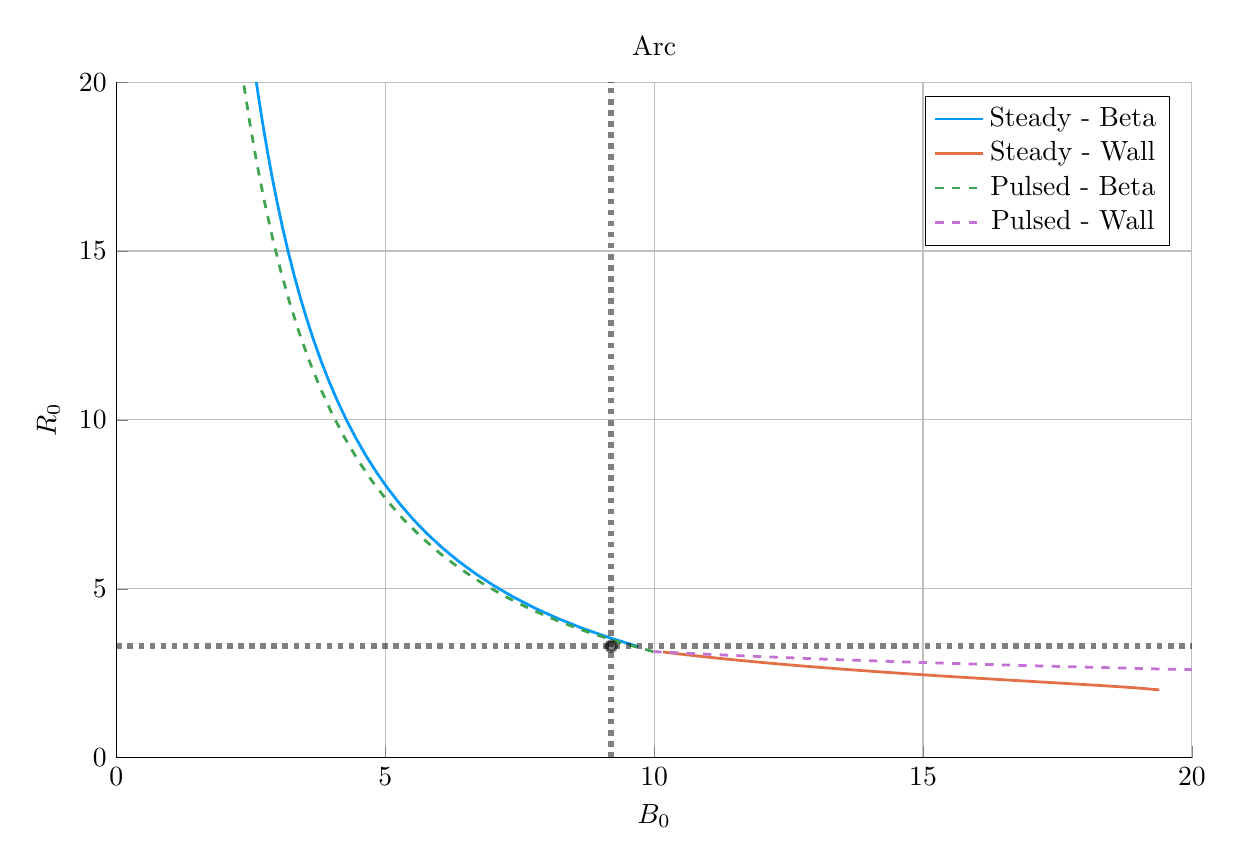
\begin{tikzpicture}[]
\begin{axis}[height = {101.6mm}, ylabel = {${R}_{0}$}, title = {Arc}, xmin = {0.0}, xmax = {20.0}, ymax = {20.0}, xlabel = {${B}_{0}$}, {unbounded coords=jump, scaled x ticks = false, xticklabel style={rotate = 0}, xmajorgrids = true, xtick = {0.0,5.0,10.0,15.0,20.0}, xticklabels = {0,5,10,15,20}, xtick align = inside, axis lines* = left, scaled y ticks = false, yticklabel style={rotate = 0}, ymajorgrids = true, ytick = {0.0,5.0,10.0,15.0,20.0}, yticklabels = {0,5,10,15,20}, ytick align = inside, axis lines* = left,     xshift = 0.0mm,
    yshift = 0.0mm,
    axis background/.style={fill={rgb,1:red,1.00000000;green,1.00000000;blue,1.00000000}}
, colorbar style={title=}}, ymin = {0.0}, width = {152.4mm}]\addplot+ [color = {rgb,1:red,0.00000000;green,0.60560316;blue,0.97868012},
draw opacity=1.0,
line width=1,
solid,mark = none,
mark size = 2.0,
mark options = {
    color = {rgb,1:red,0.00000000;green,0.00000000;blue,0.00000000}, draw opacity = 1.0,
    fill = {rgb,1:red,0.00000000;green,0.60560316;blue,0.97868012}, fill opacity = 1.0,
    line width = 1,
    rotate = 0,
    solid
}]coordinates {
(9.701206080853105, 3.2904233285656006)
(9.162315904693079, 3.553631706046861)
(8.664301107137337, 3.8315748016260343)
(8.203576462497304, 4.124583886864978)
(7.776718537485166, 4.433072975674755)
(7.380720231870917, 4.75741949036414)
(7.012886014999712, 5.097987291342331)
(6.670795005901889, 5.4551257000070565)
(6.352268997292712, 5.829168567645448)
(6.055344682097163, 6.220433393277178)
(5.778249464564785, 6.629220493040615)
(5.519380338856715, 7.05581222339423)
(5.2772854007125325, 7.500472260074458)
(5.050647625972996, 7.963444934423652)
(4.838270606140816, 8.444954628380609)
(4.639065978019038, 8.94520522910952)
(4.4520423235376105, 9.464379643936518)
(4.276295348572609, 10.002639375969222)
(4.110999177018484, 10.56012416048812)
(3.9553986195015125, 11.136951661929974)
(3.8088022956698633, 11.733217231026282)
(3.6705765055641186, 12.34899372141899)
(3.54013975965751, 12.984331364849716)
(3.4169578891619192, 13.639257703809928)
(3.30053966845824, 14.313777580345645)
(3.1904328903033052, 15.007873179535935)
(3.086220842019516, 15.721504126002731)
(2.9875191373772063, 16.45460763166718)
(2.8939728644914635, 17.207098692842226)
(2.8052540149097247, 17.97887033463821)
(2.7210591632720242, 18.7697939005645)
(2.6411073705789065, 19.579719385129263)
(2.565138287279709, 20.40847580717446)
(2.492910435164382, 21.255871621630877)
(2.4241996494611984, 22.12169516733927)
(2.3587976646588236, 23.0057151485579)
(2.296510829425685, 23.907681147764652)
(2.237158937627476, 24.827324167354146)
(2.180574163874242, 25.764357197843207)
(2.126600093288366, 26.71847581021091)
(2.075090836295778, 27.689358770027713)
(2.0259102202234582, 28.676668671060817)
(1.978931050353818, 29.68005258608471)
(1.9340344338545452, 30.69914273267572)
(1.8911091606836798, 31.733557151818793)
(1.8500511361739687, 32.78290039722107)
(1.8107628605384507, 33.846764233283025)
(1.773152951016952, 34.92472833975579)
(1.7371357028100902, 36.01636102117257)
(1.7026306853269466, 37.121219919229354)
(1.6695623706125668, 38.23885272635799)
(1.6378597911249178, 39.368797898817405)
(1.607456224302725, 40.51058536770822)
(1.5782889016090462, 41.663737246396295)
(1.5502987399539199, 42.82776853291479)
(1.5234300935954943, 44.00218780599217)
(1.4976305247952577, 45.18649791343829)
(1.4728505916614916, 46.38019665170201)
(1.4490436517578602, 47.58277743549339)
(1.4261656801829077, 48.79372995643627)
};
\addlegendentry{Steady - Beta}
\addplot+ [color = {rgb,1:red,0.88887350;green,0.43564919;blue,0.27812294},
draw opacity=1.0,
line width=1,
solid,mark = none,
mark size = 2.0,
mark options = {
    color = {rgb,1:red,0.00000000;green,0.00000000;blue,0.00000000}, draw opacity = 1.0,
    fill = {rgb,1:red,0.88887350;green,0.43564919;blue,0.27812294}, fill opacity = 1.0,
    line width = 1,
    rotate = 0,
    solid
}]coordinates {
(19.394007482712425, 2.006855814841082)
(18.932196567189358, 2.070220226465634)
(18.296989378345195, 2.1362327099649083)
(17.587029315408756, 2.2039322514902886)
(16.847882407994106, 2.272885741349308)
(16.111374502564406, 2.3427307443133163)
(15.396027314547156, 2.4132115621474344)
(14.710952688793137, 2.484165095168367)
(14.06168447794857, 2.555449485048069)
(13.450465418483889, 2.6269568263788754)
(12.877644538645335, 2.6986005527245354)
(12.342394470642008, 2.7703103261458715)
(11.843182246608265, 2.8420284550528074)
(11.376441269625893, 2.9137564749008216)
(10.944966372727551, 2.985307257194073)
(10.541663878705513, 3.056795384934831)
(10.165908182236457, 3.128148092221394)
};
\addlegendentry{Steady - Wall}
\addplot+ [color = {rgb,1:red,0.24222430;green,0.64327509;blue,0.30444865},
draw opacity=1.0,
line width=1,
dashed,mark = none,
mark size = 2.0,
mark options = {
    color = {rgb,1:red,0.00000000;green,0.00000000;blue,0.00000000}, draw opacity = 1.0,
    fill = {rgb,1:red,0.24222430;green,0.64327509;blue,0.30444865}, fill opacity = 1.0,
    line width = 1,
    rotate = 0,
    solid
}]coordinates {
(9.980483622051658, 3.1402982942956537)
(9.392786903460065, 3.3984668375583613)
(8.79273598103983, 3.7029994270206985)
(8.23820290909994, 4.029752381934837)
(7.725182218401588, 4.380005330007902)
(7.250078106370205, 4.755088191072525)
(6.80965553466646, 5.15638156809462)
(6.400998063035608, 5.585317075247801)
(6.0214713600430425, 6.043377623224966)
(5.668691517461799, 6.532097691007738)
(5.340497445229901, 7.053063624618788)
(5.034926745580058, 7.607914017422467)
(4.750194564008521, 8.198340243900201)
(4.484674995755211, 8.826087240213646)
(4.236884692979903, 9.49295465115087)
(4.00546837264544, 10.200798495308337)
(3.7891859704718387, 10.951533539957822)
(3.5869012239550364, 11.747136625739826)
(3.3975714987448393, 12.589651241396528)
(3.2202386987489797, 13.481193723261853)
(3.0540211220494466, 14.423961547290066)
(2.8981061427709687, 15.420244298711943)
(2.7517436139566023, 16.472438053930638)
(2.6142398986781377, 17.58306410230943)
(2.4849524463010138, 18.754793188384546)
(2.363284838174807, 19.990476791576892)
(2.248682232019848, 21.293187416028662)
(2.140627136740878, 22.666270490916787)
(2.038635448877246, 24.113411362836906)
(1.9422526775794744, 25.638722123308433)
(1.8510502754751532, 27.246854857488287)
(1.7646219756564088, 28.94315065234289)
(1.6825800061969869, 30.73383791051506)
(1.6045510059627948, 32.62630011975996)
(1.53017138625397, 34.629443897654504)
(1.4590817483192686, 36.754215952550474)
(1.3909197311384796, 39.01434852880224)
(1.3253102336217724, 41.42746903285954)
(1.261851128383913, 44.01681696754988)
(1.20009089049112, 46.81403058684408)
(1.1394908096975784, 49.863950342519615)
};
\addlegendentry{Pulsed - Beta}
\addplot+ [color = {rgb,1:red,0.76444018;green,0.44411178;blue,0.82429754},
draw opacity=1.0,
line width=1,
dashed,mark = none,
mark size = 2.0,
mark options = {
    color = {rgb,1:red,0.00000000;green,0.00000000;blue,0.00000000}, draw opacity = 1.0,
    fill = {rgb,1:red,0.76444018;green,0.44411178;blue,0.82429754}, fill opacity = 1.0,
    line width = 1,
    rotate = 0,
    solid
}]coordinates {
(29.27715761652869, 2.3448804182939873)
(25.4410619834368, 2.4377937236066716)
(22.158819835998365, 2.5322208586485804)
(19.342453256965573, 2.628163744265164)
(16.919364280634177, 2.7256238396687067)
(14.829378672669455, 2.8246020951898183)
(13.022412368922526, 2.9250989082568273)
(11.456617692058645, 3.0271140820266207)
(10.096901921254785, 3.1306467862637533)
(9.980483622051658, 3.1402982942956537)
};
\addlegendentry{Pulsed - Wall}
\addplot+ [color = {rgb,1:red,0.00000000;green,0.00000000;blue,0.00000000},
draw opacity=0.5,
line width=2,
dotted,mark = none,
mark size = 2.0,
mark options = {
    color = {rgb,1:red,0.00000000;green,0.00000000;blue,0.00000000}, draw opacity = 0.5,
    fill = {rgb,1:red,0.00000000;green,0.00000000;blue,0.00000000}, fill opacity = 0.5,
    line width = 1,
    rotate = 0,
    solid
},forget plot]coordinates {
(0.0, 3.3)
(20.0, 3.3)
};
\addplot+ [color = {rgb,1:red,0.00000000;green,0.00000000;blue,0.00000000},
draw opacity=0.5,
line width=2,
dotted,mark = none,
mark size = 2.0,
mark options = {
    color = {rgb,1:red,0.00000000;green,0.00000000;blue,0.00000000}, draw opacity = 0.5,
    fill = {rgb,1:red,0.00000000;green,0.00000000;blue,0.00000000}, fill opacity = 0.5,
    line width = 1,
    rotate = 0,
    solid
},forget plot]coordinates {
(9.2, 0.0)
(9.2, 20.0)
};
\addplot+[draw=none, color = {rgb,1:red,0.00000000;green,0.00000000;blue,0.00000000},
draw opacity=0.5,
line width=0,
solid,mark = *,
mark size = 2.0,
mark options = {
    color = {rgb,1:red,0.00000000;green,0.00000000;blue,0.00000000}, draw opacity = 0.5,
    fill = {rgb,1:red,0.00000000;green,0.00000000;blue,0.00000000}, fill opacity = 0.5,
    line width = 1,
    rotate = 0,
    solid
},forget plot] coordinates {
(9.2, 3.3)
};
\end{axis}

\end{tikzpicture}

    \end{adjustbox}
        \caption{$R_0$ vs $B_0$}
    \end{subfigure}
    \hfill
    \begin{subfigure}[t]{0.45\textwidth}
        \centering
    \begin{adjustbox}{width=\textwidth}
      \Large
      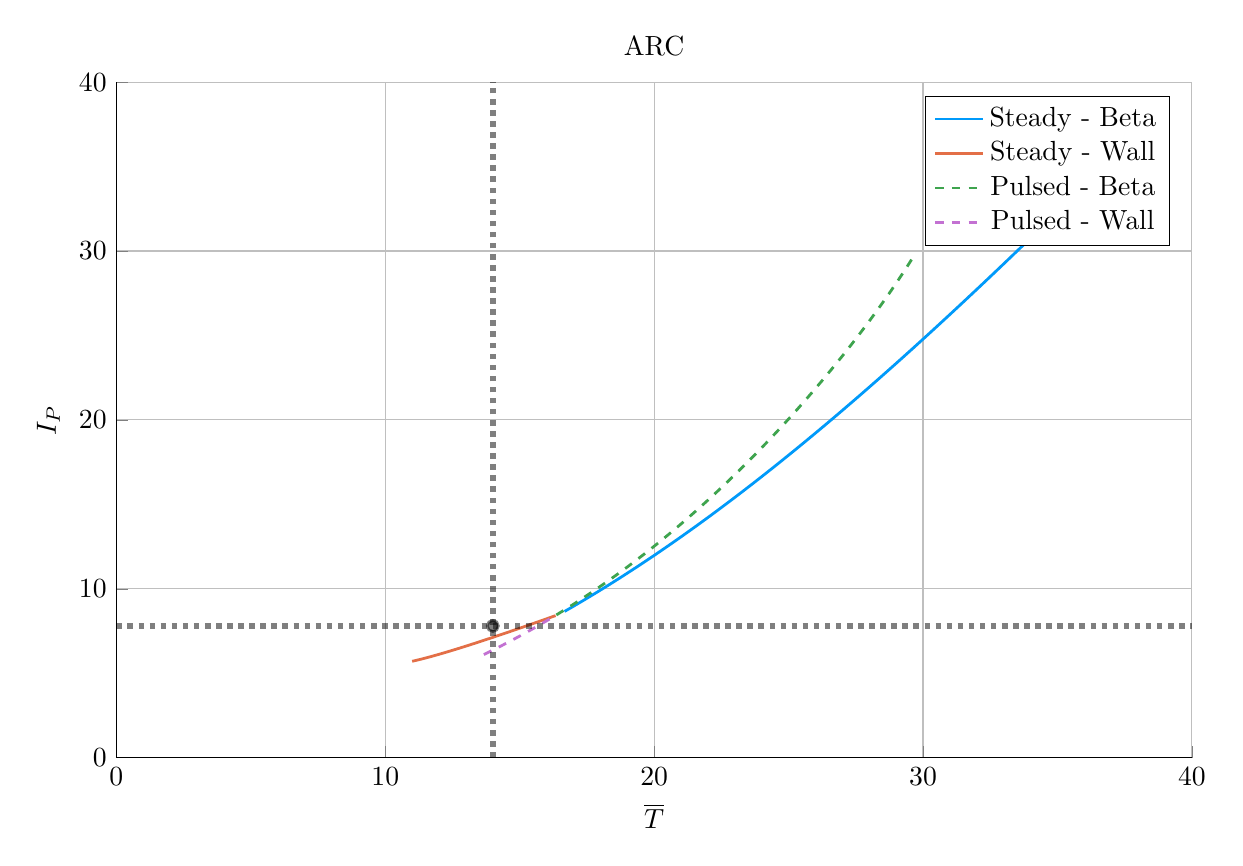
\begin{tikzpicture}[]
\begin{axis}[height = {101.6mm}, ylabel = {${I}_{P}$}, title = {ARC}, xmin = {0.0}, xmax = {40.0}, ymax = {40.0}, xlabel = {$\overline {T}$}, {unbounded coords=jump, scaled x ticks = false, xticklabel style={rotate = 0}, xmajorgrids = true, xtick = {0.0,10.0,20.0,30.0,40.0}, xticklabels = {0,10,20,30,40}, xtick align = inside, axis lines* = left, scaled y ticks = false, yticklabel style={rotate = 0}, ymajorgrids = true, ytick = {0.0,10.0,20.0,30.0,40.0}, yticklabels = {0,10,20,30,40}, ytick align = inside, axis lines* = left,     xshift = 0.0mm,
    yshift = 0.0mm,
    axis background/.style={fill={rgb,1:red,1.00000000;green,1.00000000;blue,1.00000000}}
, colorbar style={title=}}, ymin = {0.0}, width = {152.4mm}]\addplot+ [color = {rgb,1:red,0.00000000;green,0.60560316;blue,0.97868012},
draw opacity=1.0,
line width=1,
solid,mark = none,
mark size = 2.0,
mark options = {
    color = {rgb,1:red,0.00000000;green,0.00000000;blue,0.00000000}, draw opacity = 1.0,
    fill = {rgb,1:red,0.00000000;green,0.60560316;blue,0.97868012}, fill opacity = 1.0,
    line width = 1,
    rotate = 0,
    solid
}]coordinates {
(16.666666666666668, 8.658343870907427)
(17.0, 8.964855141636448)
(17.333333333333332, 9.277118721367206)
(17.666666666666668, 9.595036914426)
(18.0, 9.918585776352757)
(18.333333333333332, 10.247718935951552)
(18.666666666666668, 10.582387319200262)
(19.0, 10.922539274323045)
(19.333333333333332, 11.26812069483817)
(19.666666666666668, 11.61907514056121)
(20.0, 11.975343956529299)
(20.333333333333332, 12.336866389803589)
(20.666666666666668, 12.703579704100664)
(21.0, 13.07541929220057)
(21.333333333333332, 13.452318786079019)
(21.666666666666668, 13.834210164711733)
(22.0, 14.221023859501257)
(22.333333333333332, 14.61268885728139)
(22.666666666666668, 15.009132800857182)
(23.0, 15.410282087044596)
(23.333333333333332, 15.816061962178953)
(23.666666666666668, 16.226396615066992)
(24.0, 16.64120926736311)
(24.333333333333332, 17.060422261356294)
(24.666666666666668, 17.483957145159597)
(25.0, 17.91173475530017)
(25.333333333333332, 18.343675296712746)
(25.666666666666668, 18.77969842014449)
(26.0, 19.2197232969848)
(26.333333333333332, 19.663668691537165)
(26.666666666666668, 20.11145303075519)
(27.0, 20.562994471468567)
(27.333333333333332, 21.018210965128485)
(27.666666666666668, 21.477020320105293)
(28.0, 21.939340261574117)
(28.333333333333332, 22.405088489026962)
(28.666666666666668, 22.874182731452617)
(29.0, 23.34654080022686)
(29.333333333333332, 23.82208063975841)
(29.666666666666668, 24.300720375936947)
(30.0, 24.782378362431352)
(30.333333333333332, 25.26697322488704)
(30.666666666666668, 25.754423903072542)
(31.0, 26.244649691026318)
(31.333333333333332, 26.737570275254438)
(31.666666666666668, 27.233105771031717)
(32.0, 27.731176756857092)
(32.333333333333336, 28.23170430711659)
(32.666666666666664, 28.734610023004112)
(33.0, 29.23981606175298)
(33.333333333333336, 29.747245164229085)
(33.666666666666664, 30.256820680936514)
(34.0, 30.768466596486252)
(34.333333333333336, 31.282107552577845)
(34.666666666666664, 31.797668869543177)
(35.0, 32.31507656650066)
(35.333333333333336, 32.83425738016771)
(35.666666666666664, 33.35513878237846)
(36.0, 33.87764899635294)
(36.333333333333336, 34.40171701176134)
};
\addlegendentry{Steady - Beta}
\addplot+ [color = {rgb,1:red,0.88887350;green,0.43564919;blue,0.27812294},
draw opacity=1.0,
line width=1,
solid,mark = none,
mark size = 2.0,
mark options = {
    color = {rgb,1:red,0.00000000;green,0.00000000;blue,0.00000000}, draw opacity = 1.0,
    fill = {rgb,1:red,0.88887350;green,0.43564919;blue,0.27812294}, fill opacity = 1.0,
    line width = 1,
    rotate = 0,
    solid
}]coordinates {
(11.0, 5.705363947896813)
(11.333333333333334, 5.831631927327359)
(11.666666666666666, 5.971358416795512)
(12.0, 6.120248050030096)
(12.333333333333334, 6.27635241161913)
(12.666666666666666, 6.438084943966173)
(13.0, 6.6043437111573775)
(13.333333333333334, 6.774432932493379)
(13.666666666666666, 6.9477586358526295)
(14.0, 7.123875039246037)
(14.333333333333334, 7.302428845502918)
(14.666666666666666, 7.483135839919747)
(15.0, 7.66576464137543)
(15.333333333333334, 7.850323804140159)
(15.666666666666666, 8.036059275223955)
(16.0, 8.223435700494395)
(16.333333333333332, 8.412159667095638)
};
\addlegendentry{Steady - Wall}
\addplot+ [color = {rgb,1:red,0.24222430;green,0.64327509;blue,0.30444865},
draw opacity=1.0,
line width=1,
dashed,mark = none,
mark size = 2.0,
mark options = {
    color = {rgb,1:red,0.00000000;green,0.00000000;blue,0.00000000}, draw opacity = 1.0,
    fill = {rgb,1:red,0.24222430;green,0.64327509;blue,0.30444865}, fill opacity = 1.0,
    line width = 1,
    rotate = 0,
    solid
}]coordinates {
(16.364160609330686, 8.45211123232532)
(16.666666666666668, 8.749174237506722)
(17.0, 9.084875445329175)
(17.333333333333332, 9.429466194729264)
(17.666666666666668, 9.783065958753857)
(18.0, 10.145791398086809)
(18.333333333333332, 10.517756265001724)
(18.666666666666668, 10.899071333792335)
(19.0, 11.28984436597908)
(19.333333333333332, 11.690180120182706)
(19.666666666666668, 12.100180418434789)
(20.0, 12.519944282916168)
(20.333333333333332, 12.949568159742276)
(20.666666666666668, 13.389146249526421)
(21.0, 13.838770968145022)
(21.333333333333332, 14.298533565526986)
(21.666666666666668, 14.768524935556082)
(22.0, 15.2488366565296)
(22.333333333333332, 15.739562309352701)
(22.666666666666668, 16.240799130174846)
(23.0, 16.752650066058415)
(23.333333333333332, 17.27522631730515)
(23.666666666666668, 17.808650469386293)
(24.0, 18.353060342640163)
(24.333333333333332, 18.908613721362002)
(24.666666666666668, 19.475494169025602)
(25.0, 20.053918198206937)
(25.333333333333332, 20.644144149900036)
(25.666666666666668, 21.246483258877372)
(26.0, 21.861313557471373)
(26.333333333333332, 22.48909752802998)
(26.666666666666668, 23.130404800381292)
(27.0, 23.785941781633092)
(27.333333333333332, 24.456591033172632)
(27.666666666666668, 25.143464707502787)
(28.0, 25.84797885666414)
(28.333333333333332, 26.571959755666764)
(28.666666666666668, 27.3178012356156)
(29.0, 28.088707029156687)
(29.333333333333332, 28.889082725820668)
(29.666666666666668, 29.725209471035893)
};
\addlegendentry{Pulsed - Beta}
\addplot+ [color = {rgb,1:red,0.76444018;green,0.44411178;blue,0.82429754},
draw opacity=1.0,
line width=1,
dashed,mark = none,
mark size = 2.0,
mark options = {
    color = {rgb,1:red,0.00000000;green,0.00000000;blue,0.00000000}, draw opacity = 1.0,
    fill = {rgb,1:red,0.76444018;green,0.44411178;blue,0.82429754}, fill opacity = 1.0,
    line width = 1,
    rotate = 0,
    solid
}]coordinates {
(13.666666666666666, 6.106956435644008)
(14.0, 6.368429153074452)
(14.333333333333334, 6.637611037727747)
(14.666666666666666, 6.914640849606676)
(15.0, 7.199655680909235)
(15.333333333333334, 7.492790823032018)
(15.666666666666666, 7.794179619860046)
(16.0, 8.103953307930404)
(16.333333333333332, 8.422240844292133)
(16.364160609330686, 8.45211123232532)
};
\addlegendentry{Pulsed - Wall}
\addplot+ [color = {rgb,1:red,0.00000000;green,0.00000000;blue,0.00000000},
draw opacity=0.5,
line width=2,
dotted,mark = none,
mark size = 2.0,
mark options = {
    color = {rgb,1:red,0.00000000;green,0.00000000;blue,0.00000000}, draw opacity = 0.5,
    fill = {rgb,1:red,0.00000000;green,0.00000000;blue,0.00000000}, fill opacity = 0.5,
    line width = 1,
    rotate = 0,
    solid
},forget plot]coordinates {
(0.0, 7.8)
(40.0, 7.8)
};
\addplot+ [color = {rgb,1:red,0.00000000;green,0.00000000;blue,0.00000000},
draw opacity=0.5,
line width=2,
dotted,mark = none,
mark size = 2.0,
mark options = {
    color = {rgb,1:red,0.00000000;green,0.00000000;blue,0.00000000}, draw opacity = 0.5,
    fill = {rgb,1:red,0.00000000;green,0.00000000;blue,0.00000000}, fill opacity = 0.5,
    line width = 1,
    rotate = 0,
    solid
},forget plot]coordinates {
(14.0, 0.0)
(14.0, 40.0)
};
\addplot+[draw=none, color = {rgb,1:red,0.00000000;green,0.00000000;blue,0.00000000},
draw opacity=0.5,
line width=0,
solid,mark = *,
mark size = 2.0,
mark options = {
    color = {rgb,1:red,0.00000000;green,0.00000000;blue,0.00000000}, draw opacity = 0.5,
    fill = {rgb,1:red,0.00000000;green,0.00000000;blue,0.00000000}, fill opacity = 0.5,
    line width = 1,
    rotate = 0,
    solid
},forget plot] coordinates {
(14.0, 7.8)
};
\end{axis}

\end{tikzpicture}

    \end{adjustbox}
        \caption{$I_P$ vs $\overline T$}
    \end{subfigure}
    \hfill \hfill ~\\ ~\\ ~\\
    \caption{Arc Model Comparison} ~\\
\end{figure*}

\begin{table}[h!]
\centering  
\caption{Arc Variables}
\hfill
\begin{subtable}[t]{0.4\textwidth}
\centering  
\caption{Input Variables} ~\\
\begin{tabular}{ c|c } 

Input            & Value           \\
\hline
$H$              & 1.8             \\
$Q$              & 13.6            \\
$N_{G}$          & 0.67            \\
$\epsilon$       & 0.333          \\
$\kappa_{95}$    & 1.84            \\
$\delta_{95}$    & 0.333           \\
$\nu_{n}$        & 0.385           \\
$\nu_{T}$        & 0.929           \\
$l_{i}$          & 0.67            \\
$A$              & 2.5             \\
$Z_{eff}$        & 1.2             \\
$f_{D}$          & 0.9             \\
$\tau_{FT}$      & 1.6e9           \\
$B_{CS}$         & 12.77           \\

\end{tabular}
\end{subtable}
\hfill
\begin{subtable}[t]{0.5\textwidth}
\centering  
\caption{Output Variables} ~\\
\begin{tabular}{ c|c|c } 

Output           & Original         & Fussy.jl        \\
\hline
$R_{0}$          & 3.3              & 3.4           \\
$B_{0}$          & 9.2              & 9.5           \\
$I_{P}$          & 7.8              & 8.8           \\
$\overline n$    & 1.3              & 1.3           \\
$\overline T$    & 14.0             & 16.8           \\
$\beta_{N}$       & 0.026           & -          \\
$q_{95}$         & 7.2              & 6.1           \\
$P_{W}$          & 2.5              & 2.2           \\
$f_{BS}$         & 0.63             & 0.56          \\
$f_{CD}$         & 0.37             & 0.44          \\
$f_{IN}$         & -              & -             \\
$\volume$         & 141            & 157           \\
$P_{F}$          & 525            & 726           \\
$\eta_{CD}$      & 0.321            & 0.316          \\

\end{tabular}
\end{subtable}
\hfill
\hfill
\end{table}

\newpage

\subsection{Contrasting with the Aries Act Studies}

Moving on, the Aries Act study focuses on how steady-state reactors would look under both a conservative and optimistic perspective. This is highlighted in \cref{fig:act_h_cost}, which shows how costs decreases as the H factor is allowed to increase. Notice that for every value of H, the ACT I study (i.e. the optimistic act) has a lower cost than the design from ACT II (i.e. the conservative one).

This figure also highlights another peculiarity of the ARIES study -- a reliance on the minimum possible value of H. Note that just left of the reactor point on both plots is a highly erratic portion of the curve. As such, if even a slightly smaller value of H were used in either case, a quite distinct reactor would occur. This is not a robust way to design machines. A better approach would be to build with some safety factor -- i.e at a slightly more magical version of H. This can be seen in ARC's H-Sweep.

\begin{figure*}[h!]
    \centering
    \hfill 
    \begin{subfigure}[t]{0.4\textwidth}
        \centering
    \begin{adjustbox}{width=\textwidth}
      \Large
      \begin{tikzpicture}[]
\begin{axis}[height = {101.6mm}, ylabel = {${C}_{W}$}, title = {Act I}, xmin = {0.0}, xmax = {3.9599999999999995}, ymax = {0.1}, xlabel = {${H}$}, {unbounded coords=jump, scaled x ticks = false, xticklabel style={rotate = 0}, xmajorgrids = true, xtick = {0.0,1.0,2.0,3.0}, xticklabels = {0,1,2,3}, xtick align = inside, axis lines* = left, scaled y ticks = false, yticklabel style={rotate = 0}, ymajorgrids = true, ytick = {0.0,0.02,0.04,0.06,0.08,0.1}, yticklabels = {0.00,0.02,0.04,0.06,0.08,0.10}, ytick align = inside, axis lines* = left,     xshift = 0.0mm,
    yshift = 0.0mm,
    axis background/.style={fill={rgb,1:red,1.00000000;green,1.00000000;blue,1.00000000}}
, colorbar style={title=}}, ymin = {0.0}, width = {152.4mm}]\addplot+ [color = {rgb,1:red,0.88887350;green,0.43564919;blue,0.27812294},
draw opacity=0.7,
line width=3,
dotted,mark = none,
mark size = 2.0,
mark options = {
    color = {rgb,1:red,0.00000000;green,0.00000000;blue,0.00000000}, draw opacity = 0.7,
    fill = {rgb,1:red,0.88887350;green,0.43564919;blue,0.27812294}, fill opacity = 0.7,
    line width = 1,
    rotate = 0,
    solid
}]coordinates {
(1.65, 0.0038580882449725513)
(1.7325, 0.0034224421580344765)
(1.815, 0.0031242773601625963)
(1.8975, 0.0029076912463966475)
(1.98, 0.0027437459144664237)
(2.0625, 0.002615755758688704)
(2.145, 0.0025133725117807595)
};
\addlegendentry{$wall$}
\addplot+ [color = {rgb,1:red,0.24222430;green,0.64327509;blue,0.30444865},
draw opacity=0.7,
line width=1,
solid,mark = none,
mark size = 2.0,
mark options = {
    color = {rgb,1:red,0.00000000;green,0.00000000;blue,0.00000000}, draw opacity = 0.7,
    fill = {rgb,1:red,0.24222430;green,0.64327509;blue,0.30444865}, fill opacity = 0.7,
    line width = 1,
    rotate = 0,
    solid
}]coordinates {
(1.4025, 0.025918216479107938)
(1.485, 0.012095504772150555)
(1.5675, 0.005882239716429097)
(1.65, 0.0038447827755938714)
(1.7325, 0.0034077229105716356)
(1.815, 0.0031112188891089447)
(1.8975, 0.002896491612881698)
(1.98, 0.002734083771296579)
(2.0625, 0.002607278997942983)
(2.145, 0.002505795370579703)
(2.2275, 0.0024978293322600134)
(2.31, 0.0026050612316072053)
(2.3925, 0.002711328730788369)
(2.475, 0.0028163739703009525)
(2.5575, 0.002920119984789825)
(2.64, 0.0030223238461750735)
(2.7225, 0.003122910039550508)
(2.805, 0.003221795626029453)
(2.8875, 0.003318919864510233)
(2.97, 0.003414240640857473)
(3.0525, 0.003507731326910594)
(3.135, 0.003599378182186399)
(3.2175, 0.00368917819814934)
(3.3, 0.003777137172338829)
};
\addlegendentry{$cost$}
\addplot+ [color = {rgb,1:red,0.76444018;green,0.44411178;blue,0.82429754},
draw opacity=0.7,
line width=1,
solid,mark = none,
mark size = 2.0,
mark options = {
    color = {rgb,1:red,0.00000000;green,0.00000000;blue,0.00000000}, draw opacity = 0.7,
    fill = {rgb,1:red,0.76444018;green,0.44411178;blue,0.82429754}, fill opacity = 0.7,
    line width = 1,
    rotate = 0,
    solid
}]coordinates {
(1.4025, 0.02636776101728183)
(1.485, 0.018483166138998787)
(1.5675, 0.007170526433976295)
(1.65, 0.003841721357482374)
(1.7325, 0.0034053745614292777)
(1.815, 0.0031097242744622163)
(1.8975, 0.002895546190157591)
(1.98, 0.0027334738346990873)
(2.0625, 0.002606876408558846)
(2.145, 0.0025055240752749086)
(2.2275, 0.0024978197141057924)
(2.31, 0.0026050530799257014)
(2.3925, 0.0027113218095688846)
(2.475, 0.0028164020534254693)
(2.5575, 0.0029201149972198264)
(2.64, 0.0030223196276555316)
(2.7225, 0.003122906476745389)
(2.805, 0.0032217926032687013)
(2.8875, 0.0033189173512138603)
(2.97, 0.0034142385345432096)
(3.0525, 0.0035077295453675586)
(3.135, 0.0035993767225118564)
(3.2175, 0.003689176968945425)
(3.3, 0.0037771361544507143)
};
\addlegendentry{$W_M$}
\addplot+ [color = {rgb,1:red,0.67554396;green,0.55566233;blue,0.09423434},
draw opacity=1.0,
line width=1,
dashed,mark = none,
mark size = 2.0,
mark options = {
    color = {rgb,1:red,0.00000000;green,0.00000000;blue,0.00000000}, draw opacity = 1.0,
    fill = {rgb,1:red,0.67554396;green,0.55566233;blue,0.09423434}, fill opacity = 1.0,
    line width = 1,
    rotate = 0,
    solid
},forget plot]coordinates {
(1.65, 0.0)
(1.65, 0.1)
};
\addplot+ [color = {rgb,1:red,0.00000048;green,0.66575898;blue,0.68099695},
draw opacity=1.0,
line width=1,
dashed,mark = none,
mark size = 2.0,
mark options = {
    color = {rgb,1:red,0.00000000;green,0.00000000;blue,0.00000000}, draw opacity = 1.0,
    fill = {rgb,1:red,0.00000048;green,0.66575898;blue,0.68099695}, fill opacity = 1.0,
    line width = 1,
    rotate = 0,
    solid
},forget plot]coordinates {
(0.0, 0.0)
(0.0, 0.1)
};
\addplot+ [color = {rgb,1:red,0.00000048;green,0.66575898;blue,0.68099695},
draw opacity=1.0,
line width=1,
dashed,mark = none,
mark size = 2.0,
mark options = {
    color = {rgb,1:red,0.00000000;green,0.00000000;blue,0.00000000}, draw opacity = 1.0,
    fill = {rgb,1:red,0.00000048;green,0.66575898;blue,0.68099695}, fill opacity = 1.0,
    line width = 1,
    rotate = 0,
    solid
},forget plot]coordinates {
(3.3, 0.0)
(3.3, 0.1)
};
\end{axis}

\end{tikzpicture}

    \end{adjustbox}
        \caption{Act I H Sweep}
    \end{subfigure}
    \hfill
    \begin{subfigure}[t]{0.4\textwidth}
        \centering
    \begin{adjustbox}{width=\textwidth}
      \Large
      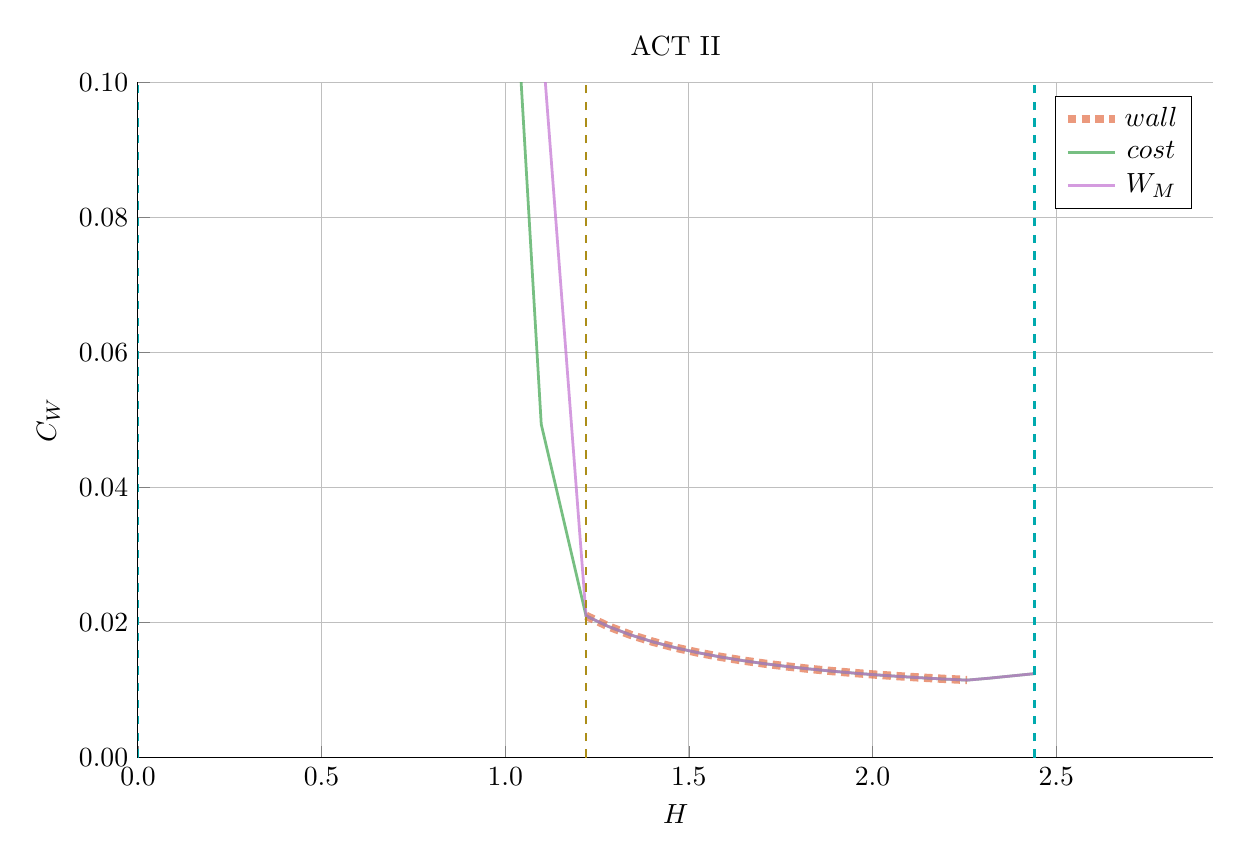
\begin{tikzpicture}[]
\begin{axis}[height = {101.6mm}, ylabel = {${C}_{W}$}, title = {ACT II}, xmin = {0.0}, xmax = {2.928}, ymax = {0.1}, xlabel = {${H}$}, {unbounded coords=jump, scaled x ticks = false, xticklabel style={rotate = 0}, xmajorgrids = true, xtick = {0.0,0.5,1.0,1.5,2.0,2.5}, xticklabels = {0.0,0.5,1.0,1.5,2.0,2.5}, xtick align = inside, axis lines* = left, scaled y ticks = false, yticklabel style={rotate = 0}, ymajorgrids = true, ytick = {0.0,0.02,0.04,0.06,0.08,0.1}, yticklabels = {0.00,0.02,0.04,0.06,0.08,0.10}, ytick align = inside, axis lines* = left,     xshift = 0.0mm,
    yshift = 0.0mm,
    axis background/.style={fill={rgb,1:red,1.00000000;green,1.00000000;blue,1.00000000}}
, colorbar style={title=}}, ymin = {0.0}, width = {152.4mm}]\addplot+ [color = {rgb,1:red,0.88887350;green,0.43564919;blue,0.27812294},
draw opacity=0.7,
line width=3,
dotted,mark = none,
mark size = 2.0,
mark options = {
    color = {rgb,1:red,0.00000000;green,0.00000000;blue,0.00000000}, draw opacity = 0.7,
    fill = {rgb,1:red,0.88887350;green,0.43564919;blue,0.27812294}, fill opacity = 0.7,
    line width = 1,
    rotate = 0,
    solid
}]coordinates {
(1.22, 0.021005512518330174)
(1.281, 0.01942744270360855)
(1.342, 0.018170389811630824)
(1.403, 0.017139710886836464)
(1.464, 0.01627794436788193)
(1.525, 0.015546450836866612)
(1.586, 0.014919600022944367)
(1.647, 0.014377436937475022)
(1.708, 0.013905581766222853)
(1.769, 0.01349265356023887)
(1.83, 0.013129558656358339)
(1.891, 0.01280891244140467)
(1.952, 0.012524569645508304)
(2.013, 0.01227184717788876)
(2.074, 0.012046102834086084)
(2.135, 0.01184360516877147)
(2.196, 0.011661349792575638)
(2.257, 0.011496773538316084)
};
\addlegendentry{$wall$}
\addplot+ [color = {rgb,1:red,0.24222430;green,0.64327509;blue,0.30444865},
draw opacity=0.7,
line width=1,
solid,mark = none,
mark size = 2.0,
mark options = {
    color = {rgb,1:red,0.00000000;green,0.00000000;blue,0.00000000}, draw opacity = 0.7,
    fill = {rgb,1:red,0.24222430;green,0.64327509;blue,0.30444865}, fill opacity = 0.7,
    line width = 1,
    rotate = 0,
    solid
}]coordinates {
(1.037, 0.10576482650233505)
(1.098, 0.04935829436307264)
(1.22, 0.020990970199014802)
(1.281, 0.0194129595370893)
(1.342, 0.01815662533322952)
(1.403, 0.01712672739309554)
(1.464, 0.016265578765863785)
(1.525, 0.015534719386234706)
(1.586, 0.014908297877268767)
(1.647, 0.014366575271189693)
(1.708, 0.013895114510245749)
(1.769, 0.013482541510434981)
(1.83, 0.013119766959557726)
(1.891, 0.012796621459369077)
(1.952, 0.012503284271399288)
(2.013, 0.012246990247871287)
(2.074, 0.012019443303647051)
(2.135, 0.011815835760118812)
(2.196, 0.011632962604193957)
(2.257, 0.011474758216077388)
(2.318, 0.011765579200211946)
(2.379, 0.012101340215422274)
(2.44, 0.012432978177363389)
};
\addlegendentry{$cost$}
\addplot+ [color = {rgb,1:red,0.76444018;green,0.44411178;blue,0.82429754},
draw opacity=0.7,
line width=1,
solid,mark = none,
mark size = 2.0,
mark options = {
    color = {rgb,1:red,0.00000000;green,0.00000000;blue,0.00000000}, draw opacity = 0.7,
    fill = {rgb,1:red,0.76444018;green,0.44411178;blue,0.82429754}, fill opacity = 0.7,
    line width = 1,
    rotate = 0,
    solid
}]coordinates {
(1.098, 0.10789687618345375)
(1.22, 0.020993563020398034)
(1.281, 0.019414381524971283)
(1.342, 0.018157569810455732)
(1.403, 0.017127496371177657)
(1.464, 0.016266077641847662)
(1.525, 0.015535219465132215)
(1.586, 0.014908546212398566)
(1.647, 0.014366740003006752)
(1.708, 0.013895218421357018)
(1.769, 0.01348260263682947)
(1.83, 0.013119799308255348)
(1.891, 0.0127993859843838)
(1.952, 0.012506614611284711)
(2.013, 0.01224686415179682)
(2.074, 0.012019222925033022)
(2.135, 0.011815568425293648)
(2.196, 0.011632678053496345)
(2.257, 0.011474127813480542)
(2.318, 0.011765572318494604)
(2.379, 0.012101333413489)
(2.44, 0.012432971811628111)
};
\addlegendentry{$W_M$}
\addplot+ [color = {rgb,1:red,0.67554396;green,0.55566233;blue,0.09423434},
draw opacity=1.0,
line width=1,
dashed,mark = none,
mark size = 2.0,
mark options = {
    color = {rgb,1:red,0.00000000;green,0.00000000;blue,0.00000000}, draw opacity = 1.0,
    fill = {rgb,1:red,0.67554396;green,0.55566233;blue,0.09423434}, fill opacity = 1.0,
    line width = 1,
    rotate = 0,
    solid
},forget plot]coordinates {
(1.22, 0.0)
(1.22, 0.1)
};
\addplot+ [color = {rgb,1:red,0.00000048;green,0.66575898;blue,0.68099695},
draw opacity=1.0,
line width=1,
dashed,mark = none,
mark size = 2.0,
mark options = {
    color = {rgb,1:red,0.00000000;green,0.00000000;blue,0.00000000}, draw opacity = 1.0,
    fill = {rgb,1:red,0.00000048;green,0.66575898;blue,0.68099695}, fill opacity = 1.0,
    line width = 1,
    rotate = 0,
    solid
},forget plot]coordinates {
(0.0, 0.0)
(0.0, 0.1)
};
\addplot+ [color = {rgb,1:red,0.00000048;green,0.66575898;blue,0.68099695},
draw opacity=1.0,
line width=1,
dashed,mark = none,
mark size = 2.0,
mark options = {
    color = {rgb,1:red,0.00000000;green,0.00000000;blue,0.00000000}, draw opacity = 1.0,
    fill = {rgb,1:red,0.00000048;green,0.66575898;blue,0.68099695}, fill opacity = 1.0,
    line width = 1,
    rotate = 0,
    solid
},forget plot]coordinates {
(2.44, 0.0)
(2.44, 0.1)
};
\end{axis}

\end{tikzpicture}

    \end{adjustbox}
        \caption{Act II H Sweep}
    \end{subfigure}
    \hfill \hfill ~\\ ~\\ ~\\
    \begin{subfigure}[t]{0.4\textwidth}
        \centering
		\begin{adjustbox}{width=\textwidth}
			\Large
			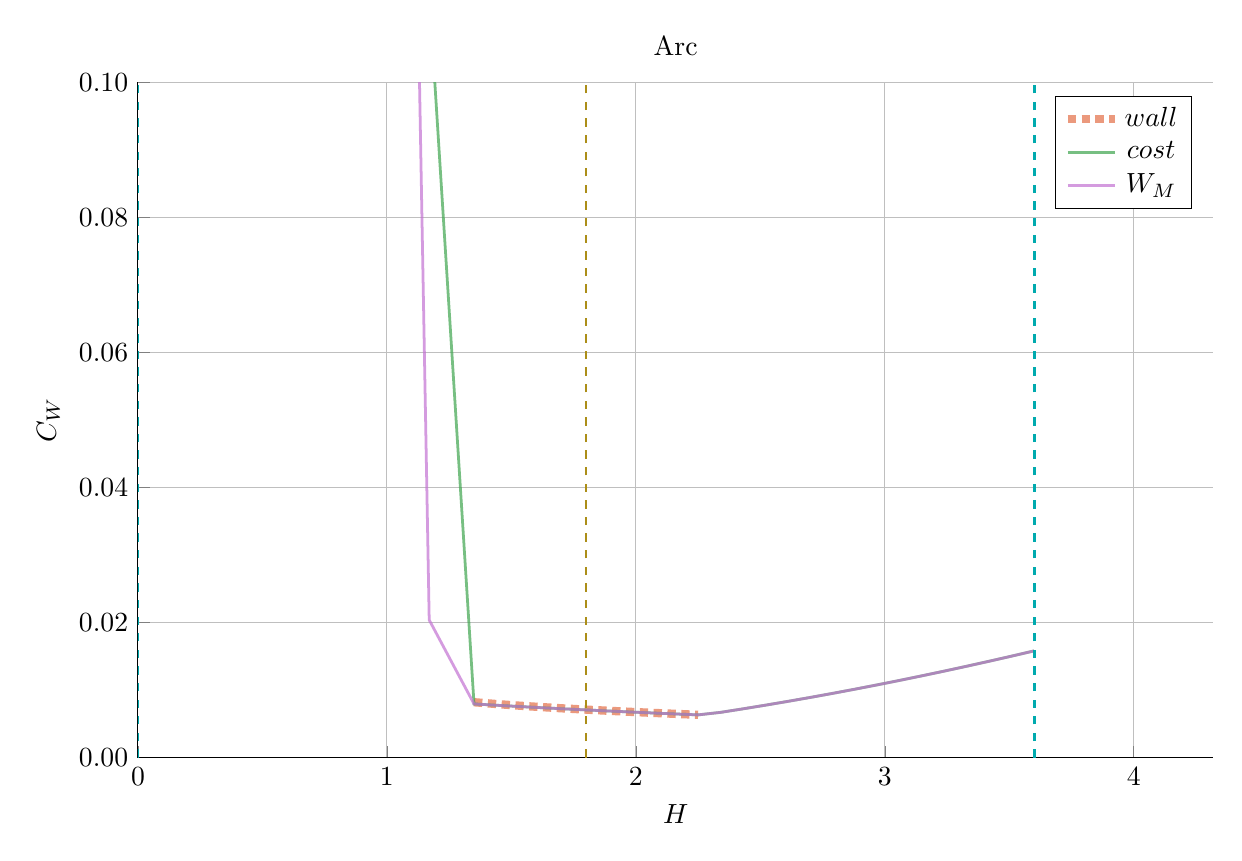
\begin{tikzpicture}[]
\begin{axis}[height = {101.6mm}, ylabel = {${C}_{W}$}, title = {Arc}, xmin = {0.0}, xmax = {4.32}, ymax = {0.1}, xlabel = {${H}$}, {unbounded coords=jump, scaled x ticks = false, xticklabel style={rotate = 0}, xmajorgrids = true, xtick = {0.0,1.0,2.0,3.0,4.0}, xticklabels = {0,1,2,3,4}, xtick align = inside, axis lines* = left, scaled y ticks = false, yticklabel style={rotate = 0}, ymajorgrids = true, ytick = {0.0,0.02,0.04,0.06,0.08,0.1}, yticklabels = {0.00,0.02,0.04,0.06,0.08,0.10}, ytick align = inside, axis lines* = left,     xshift = 0.0mm,
    yshift = 0.0mm,
    axis background/.style={fill={rgb,1:red,1.00000000;green,1.00000000;blue,1.00000000}}
, colorbar style={title=}}, ymin = {0.0}, width = {152.4mm}]\addplot+ [color = {rgb,1:red,0.88887350;green,0.43564919;blue,0.27812294},
draw opacity=0.7,
line width=3,
dotted,mark = none,
mark size = 2.0,
mark options = {
    color = {rgb,1:red,0.00000000;green,0.00000000;blue,0.00000000}, draw opacity = 0.7,
    fill = {rgb,1:red,0.88887350;green,0.43564919;blue,0.27812294}, fill opacity = 0.7,
    line width = 1,
    rotate = 0,
    solid
}]coordinates {
(1.35, 0.008207241762396246)
(1.44, 0.00793667759257354)
(1.53, 0.0076997912429461225)
(1.62, 0.007486816554981894)
(1.71, 0.007291648689881567)
(1.8, 0.007110333347796811)
(1.89, 0.006940248814588952)
(1.98, 0.006779633349026309)
(2.07, 0.006627297197584387)
(2.16, 0.006482438866566955)
(2.25, 0.006344768968841929)
};
\addlegendentry{$wall$}
\addplot+ [color = {rgb,1:red,0.24222430;green,0.64327509;blue,0.30444865},
draw opacity=0.7,
line width=1,
solid,mark = none,
mark size = 2.0,
mark options = {
    color = {rgb,1:red,0.00000000;green,0.00000000;blue,0.00000000}, draw opacity = 0.7,
    fill = {rgb,1:red,0.24222430;green,0.64327509;blue,0.30444865}, fill opacity = 0.7,
    line width = 1,
    rotate = 0,
    solid
}]coordinates {
(1.08, 0.1656933786109522)
(1.35, 0.007956028922350611)
(1.44, 0.007759662745290108)
(1.53, 0.007574913322065527)
(1.62, 0.00739885086770846)
(1.71, 0.0072297906534508185)
(1.8, 0.007066784363464752)
(1.89, 0.00690932755478892)
(1.98, 0.006757201835765392)
(2.07, 0.006610359300650354)
(2.16, 0.0064688545800951625)
(2.25, 0.006332913629979953)
(2.34, 0.00670268792962123)
(2.43, 0.0072243580642261445)
(2.52, 0.007766406785339575)
(2.61, 0.008328785580854575)
(2.7, 0.008911412315791628)
(2.79, 0.00951417119398493)
(2.88, 0.010136912409268534)
(2.97, 0.010779452862615483)
(3.06, 0.011441576670944502)
(3.15, 0.012123036438828786)
(3.24, 0.012823554577929932)
(3.33, 0.0135428254017145)
(3.42, 0.014280516598644705)
(3.51, 0.015036271676563144)
(3.6, 0.01580971210009804)
};
\addlegendentry{$cost$}
\addplot+ [color = {rgb,1:red,0.76444018;green,0.44411178;blue,0.82429754},
draw opacity=0.7,
line width=1,
solid,mark = none,
mark size = 2.0,
mark options = {
    color = {rgb,1:red,0.00000000;green,0.00000000;blue,0.00000000}, draw opacity = 0.7,
    fill = {rgb,1:red,0.76444018;green,0.44411178;blue,0.82429754}, fill opacity = 0.7,
    line width = 1,
    rotate = 0,
    solid
}]coordinates {
(1.08, 0.20419403931121408)
(1.17, 0.02038194154635263)
(1.35, 0.007952462446561684)
(1.44, 0.007756882763096937)
(1.53, 0.007572765485693452)
(1.62, 0.007397214242173672)
(1.71, 0.007228584574974498)
(1.8, 0.007065962995902896)
(1.89, 0.006908746287963411)
(1.98, 0.006756833824238413)
(2.07, 0.0066101524637499)
(2.16, 0.006468686518064958)
(2.25, 0.006332754951862069)
(2.34, 0.00670262687626648)
(2.43, 0.007224172350640052)
(2.52, 0.007766066748915404)
(2.61, 0.008328266004035769)
(2.7, 0.008910694013555907)
(2.79, 0.009513241975770496)
(2.88, 0.010135768084513136)
(2.97, 0.010778097603257038)
(3.06, 0.011440023505553681)
(3.15, 0.01212130721887041)
(3.24, 0.012821680052634414)
(3.33, 0.013540844476435391)
(3.42, 0.014278476232750113)
(3.51, 0.015034225935616565)
(3.6, 0.01580772161808181)
};
\addlegendentry{$W_M$}
\addplot+ [color = {rgb,1:red,0.67554396;green,0.55566233;blue,0.09423434},
draw opacity=1.0,
line width=1,
dashed,mark = none,
mark size = 2.0,
mark options = {
    color = {rgb,1:red,0.00000000;green,0.00000000;blue,0.00000000}, draw opacity = 1.0,
    fill = {rgb,1:red,0.67554396;green,0.55566233;blue,0.09423434}, fill opacity = 1.0,
    line width = 1,
    rotate = 0,
    solid
},forget plot]coordinates {
(1.8, 0.0)
(1.8, 0.1)
};
\addplot+ [color = {rgb,1:red,0.00000048;green,0.66575898;blue,0.68099695},
draw opacity=1.0,
line width=1,
dashed,mark = none,
mark size = 2.0,
mark options = {
    color = {rgb,1:red,0.00000000;green,0.00000000;blue,0.00000000}, draw opacity = 1.0,
    fill = {rgb,1:red,0.00000048;green,0.66575898;blue,0.68099695}, fill opacity = 1.0,
    line width = 1,
    rotate = 0,
    solid
},forget plot]coordinates {
(0.0, 0.0)
(0.0, 0.1)
};
\addplot+ [color = {rgb,1:red,0.00000048;green,0.66575898;blue,0.68099695},
draw opacity=1.0,
line width=1,
dashed,mark = none,
mark size = 2.0,
mark options = {
    color = {rgb,1:red,0.00000000;green,0.00000000;blue,0.00000000}, draw opacity = 1.0,
    fill = {rgb,1:red,0.00000048;green,0.66575898;blue,0.68099695}, fill opacity = 1.0,
    line width = 1,
    rotate = 0,
    solid
},forget plot]coordinates {
(3.6, 0.0)
(3.6, 0.1)
};
\end{axis}

\end{tikzpicture}

		\end{adjustbox}
        \caption{Arc H Sweep}
    \end{subfigure} ~\\ ~\\ ~\\
    \caption{Act Studies Cost Dependence on the H Factor} ~\\    
	\label{fig:act_h_cost}
\end{figure*}

\newpage 

\subsubsection{Act I -- Advanced Physics and Engineering}

Act 1 is the ARIES study that assumes advanced physics and engineering design parameters. Although this paper's model does a good job matching the results from their paper, it does show what optimistic design really means. As can be seen, this design actually only surpasses the minimum possible toroidal field strength by as less than a Tesla! Practically, this means the reactor is barely realizable.

\begin{figure*}[h!]
    \centering
    \hfill 
    \begin{subfigure}[t]{0.45\textwidth}
        \centering
    \begin{adjustbox}{width=\textwidth}
      \Large
      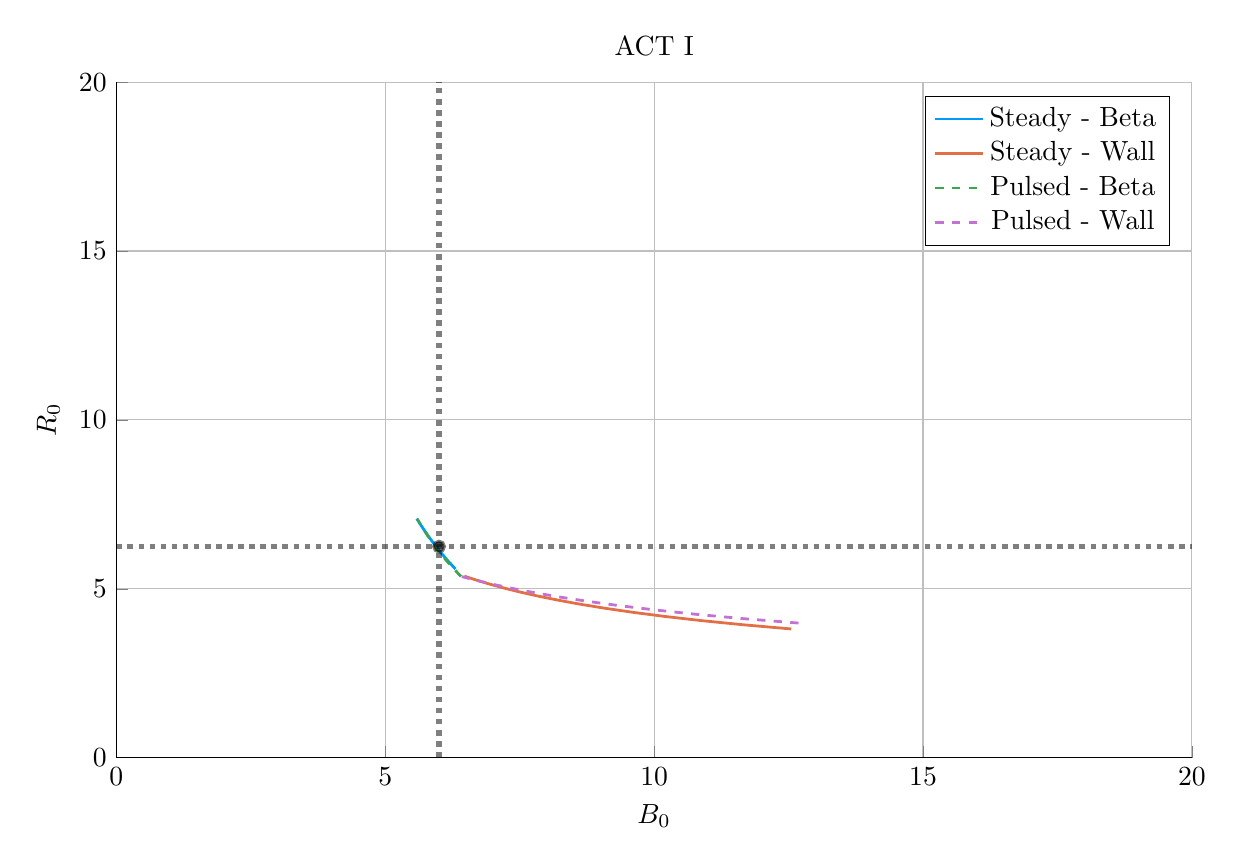
\begin{tikzpicture}[]
\begin{axis}[height = {101.6mm}, ylabel = {${R}_{0}$}, title = {ACT I}, xmin = {0.0}, xmax = {20.0}, ymax = {20.0}, xlabel = {${B}_{0}$}, {unbounded coords=jump, scaled x ticks = false, xticklabel style={rotate = 0}, xmajorgrids = true, xtick = {0.0,5.0,10.0,15.0,20.0}, xticklabels = {0,5,10,15,20}, xtick align = inside, axis lines* = left, scaled y ticks = false, yticklabel style={rotate = 0}, ymajorgrids = true, ytick = {0.0,5.0,10.0,15.0,20.0}, yticklabels = {0,5,10,15,20}, ytick align = inside, axis lines* = left,     xshift = 0.0mm,
    yshift = 0.0mm,
    axis background/.style={fill={rgb,1:red,1.00000000;green,1.00000000;blue,1.00000000}}
, colorbar style={title=}}, ymin = {0.0}, width = {152.4mm}]\addplot+ [color = {rgb,1:red,0.00000000;green,0.60560316;blue,0.97868012},
draw opacity=1.0,
line width=1,
solid,mark = none,
mark size = 2.0,
mark options = {
    color = {rgb,1:red,0.00000000;green,0.00000000;blue,0.00000000}, draw opacity = 1.0,
    fill = {rgb,1:red,0.00000000;green,0.60560316;blue,0.97868012}, fill opacity = 1.0,
    line width = 1,
    rotate = 0,
    solid
}]coordinates {
(6.30336807958207, 5.587199391496101)
(6.162193069273141, 5.831838137107903)
(6.030717178404645, 6.078157823726375)
(5.908065509576601, 6.325994353145188)
(5.793464904530972, 6.57518910191267)
(5.686229631357383, 6.825588847053452)
(5.585749511271037, 7.077045564754442)
};
\addlegendentry{Steady - Beta}
\addplot+ [color = {rgb,1:red,0.88887350;green,0.43564919;blue,0.27812294},
draw opacity=1.0,
line width=1,
solid,mark = none,
mark size = 2.0,
mark options = {
    color = {rgb,1:red,0.00000000;green,0.00000000;blue,0.00000000}, draw opacity = 1.0,
    fill = {rgb,1:red,0.88887350;green,0.43564919;blue,0.27812294}, fill opacity = 1.0,
    line width = 1,
    rotate = 0,
    solid
}]coordinates {
(12.549536249695134, 3.8108352245940957)
(11.658754653696462, 3.934083270736017)
(10.883719833507003, 4.057046546594516)
(10.206258129789394, 4.179626810883221)
(9.611335769312953, 4.301750356443285)
(9.086446934250878, 4.423366229113912)
(8.62129895070743, 4.544434218016914)
(8.207216040989662, 4.6649335402400025)
(7.837119555085499, 4.78484200403474)
(7.505047858717157, 4.9041467319817595)
(7.20604322925957, 5.022835870779136)
(6.935884710193303, 5.1409045607718795)
(6.691016583192173, 5.258349129805506)
(6.468415485086983, 5.375167957409874)
};
\addlegendentry{Steady - Wall}
\addplot+ [color = {rgb,1:red,0.24222430;green,0.64327509;blue,0.30444865},
draw opacity=1.0,
line width=1,
dashed,mark = none,
mark size = 2.0,
mark options = {
    color = {rgb,1:red,0.00000000;green,0.00000000;blue,0.00000000}, draw opacity = 1.0,
    fill = {rgb,1:red,0.24222430;green,0.64327509;blue,0.30444865}, fill opacity = 1.0,
    line width = 1,
    rotate = 0,
    solid
}]coordinates {
(6.408263337806559, 5.366131328829866)
(6.408263337806564, 5.366131328829862)
(6.385466513301022, 5.402805883604879)
(6.245492502072912, 5.638974714472524)
(6.116010320461132, 5.875875066688821)
(5.9960421481916395, 6.113307727774442)
(5.884727159112828, 6.351082733498888)
(5.781304768121868, 6.589019058920955)
(5.685100648450046, 6.826944315253105)
(5.595515000321003, 7.064694456596427)
};
\addlegendentry{Pulsed - Beta}
\addplot+ [color = {rgb,1:red,0.76444018;green,0.44411178;blue,0.82429754},
draw opacity=1.0,
line width=1,
dashed,mark = none,
mark size = 2.0,
mark options = {
    color = {rgb,1:red,0.00000000;green,0.00000000;blue,0.00000000}, draw opacity = 1.0,
    fill = {rgb,1:red,0.76444018;green,0.44411178;blue,0.82429754}, fill opacity = 1.0,
    line width = 1,
    rotate = 0,
    solid
}]coordinates {
(12.684248532650473, 3.9847907768802657)
(11.66307871570063, 4.114684512780648)
(10.781888309639141, 4.244124103742294)
(10.016282491385791, 4.373086052625054)
(9.346943280276514, 4.501549309887817)
(8.758420158941194, 4.6294950281779785)
(8.238241792953433, 4.756906348757686)
(7.776255600865612, 4.883768212546736)
(7.364131118520045, 5.010067192354689)
(6.994982564641668, 5.135791343697217)
(6.66307916140573, 5.260930071474144)
(6.408263337806559, 5.366131328829866)
(6.408263337806564, 5.366131328829862)
};
\addlegendentry{Pulsed - Wall}
\addplot+ [color = {rgb,1:red,0.00000000;green,0.00000000;blue,0.00000000},
draw opacity=0.5,
line width=2,
dotted,mark = none,
mark size = 2.0,
mark options = {
    color = {rgb,1:red,0.00000000;green,0.00000000;blue,0.00000000}, draw opacity = 0.5,
    fill = {rgb,1:red,0.00000000;green,0.00000000;blue,0.00000000}, fill opacity = 0.5,
    line width = 1,
    rotate = 0,
    solid
},forget plot]coordinates {
(0.0, 6.25)
(20.0, 6.25)
};
\addplot+ [color = {rgb,1:red,0.00000000;green,0.00000000;blue,0.00000000},
draw opacity=0.5,
line width=2,
dotted,mark = none,
mark size = 2.0,
mark options = {
    color = {rgb,1:red,0.00000000;green,0.00000000;blue,0.00000000}, draw opacity = 0.5,
    fill = {rgb,1:red,0.00000000;green,0.00000000;blue,0.00000000}, fill opacity = 0.5,
    line width = 1,
    rotate = 0,
    solid
},forget plot]coordinates {
(6.0, 0.0)
(6.0, 20.0)
};
\addplot+[draw=none, color = {rgb,1:red,0.00000000;green,0.00000000;blue,0.00000000},
draw opacity=0.5,
line width=0,
solid,mark = *,
mark size = 2.0,
mark options = {
    color = {rgb,1:red,0.00000000;green,0.00000000;blue,0.00000000}, draw opacity = 0.5,
    fill = {rgb,1:red,0.00000000;green,0.00000000;blue,0.00000000}, fill opacity = 0.5,
    line width = 1,
    rotate = 0,
    solid
},forget plot] coordinates {
(6.0, 6.25)
};
\end{axis}

\end{tikzpicture}

    \end{adjustbox}
        \caption{$R_0$ vs $B_0$}
    \end{subfigure}
    \hfill
    \begin{subfigure}[t]{0.45\textwidth}
        \centering
    \begin{adjustbox}{width=\textwidth}
      \Large
      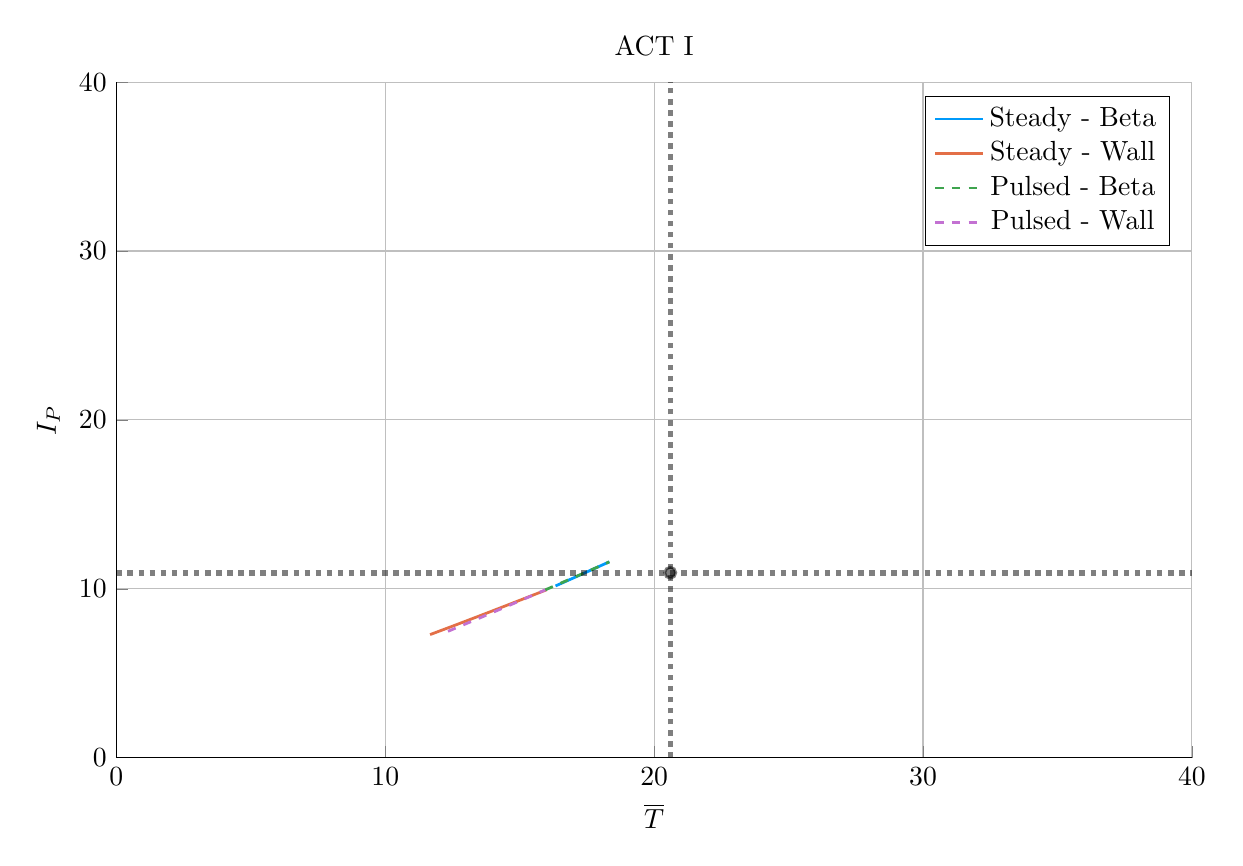
\begin{tikzpicture}[]
\begin{axis}[height = {101.6mm}, ylabel = {${I}_{P}$}, title = {ACT I}, xmin = {0.0}, xmax = {40.0}, ymax = {40.0}, xlabel = {$\overline {T}$}, {unbounded coords=jump, scaled x ticks = false, xticklabel style={rotate = 0}, xmajorgrids = true, xtick = {0.0,10.0,20.0,30.0,40.0}, xticklabels = {0,10,20,30,40}, xtick align = inside, axis lines* = left, scaled y ticks = false, yticklabel style={rotate = 0}, ymajorgrids = true, ytick = {0.0,10.0,20.0,30.0,40.0}, yticklabels = {0,10,20,30,40}, ytick align = inside, axis lines* = left,     xshift = 0.0mm,
    yshift = 0.0mm,
    axis background/.style={fill={rgb,1:red,1.00000000;green,1.00000000;blue,1.00000000}}
, colorbar style={title=}}, ymin = {0.0}, width = {152.4mm}]\addplot+ [color = {rgb,1:red,0.00000000;green,0.60560316;blue,0.97868012},
draw opacity=1.0,
line width=1,
solid,mark = none,
mark size = 2.0,
mark options = {
    color = {rgb,1:red,0.00000000;green,0.00000000;blue,0.00000000}, draw opacity = 1.0,
    fill = {rgb,1:red,0.00000000;green,0.60560316;blue,0.97868012}, fill opacity = 1.0,
    line width = 1,
    rotate = 0,
    solid
}]coordinates {
(16.333333333333332, 10.169194435531358)
(16.666666666666668, 10.405057509328124)
(17.0, 10.641905327194731)
(17.333333333333332, 10.87971637136811)
(17.666666666666668, 11.11846917050157)
(18.0, 11.358142407296011)
(18.333333333333332, 11.598714938197329)
};
\addlegendentry{Steady - Beta}
\addplot+ [color = {rgb,1:red,0.88887350;green,0.43564919;blue,0.27812294},
draw opacity=1.0,
line width=1,
solid,mark = none,
mark size = 2.0,
mark options = {
    color = {rgb,1:red,0.00000000;green,0.00000000;blue,0.00000000}, draw opacity = 1.0,
    fill = {rgb,1:red,0.88887350;green,0.43564919;blue,0.27812294}, fill opacity = 1.0,
    line width = 1,
    rotate = 0,
    solid
}]coordinates {
(11.666666666666666, 7.287903136887)
(12.0, 7.486025430610099)
(12.333333333333334, 7.685696663157812)
(12.666666666666666, 7.886645361110723)
(13.0, 8.08866940687473)
(13.333333333333334, 8.291629426976055)
(13.666666666666666, 8.495414075666067)
(14.0, 8.699964056113311)
(14.333333333333334, 8.905213556979005)
(14.666666666666666, 9.111120468746519)
(15.0, 9.31764336053339)
(15.333333333333334, 9.524758318501357)
(15.666666666666666, 9.732442959434447)
(16.0, 9.940679052729761)
};
\addlegendentry{Steady - Wall}
\addplot+ [color = {rgb,1:red,0.24222430;green,0.64327509;blue,0.30444865},
draw opacity=1.0,
line width=1,
dashed,mark = none,
mark size = 2.0,
mark options = {
    color = {rgb,1:red,0.00000000;green,0.00000000;blue,0.00000000}, draw opacity = 1.0,
    fill = {rgb,1:red,0.24222430;green,0.64327509;blue,0.30444865}, fill opacity = 1.0,
    line width = 1,
    rotate = 0,
    solid
}]coordinates {
(15.948125117373092, 9.933500150990564)
(15.9481251173731, 9.933500150990564)
(16.0, 9.969282740147014)
(16.333333333333332, 10.199548426407084)
(16.666666666666668, 10.430379144484162)
(17.0, 10.661750348679098)
(17.333333333333332, 10.893638132753678)
(17.666666666666668, 11.126019229767902)
(18.0, 11.358871009413285)
(18.333333333333332, 11.592171473618816)
};
\addlegendentry{Pulsed - Beta}
\addplot+ [color = {rgb,1:red,0.76444018;green,0.44411178;blue,0.82429754},
draw opacity=1.0,
line width=1,
dashed,mark = none,
mark size = 2.0,
mark options = {
    color = {rgb,1:red,0.00000000;green,0.00000000;blue,0.00000000}, draw opacity = 1.0,
    fill = {rgb,1:red,0.76444018;green,0.44411178;blue,0.82429754}, fill opacity = 1.0,
    line width = 1,
    rotate = 0,
    solid
}]coordinates {
(12.333333333333334, 7.481290856821823)
(12.666666666666666, 7.703549290655078)
(13.0, 7.92668121689452)
(13.333333333333334, 8.15065615613957)
(13.666666666666666, 8.375443966327172)
(14.0, 8.601014900773066)
(14.333333333333334, 8.82733966430566)
(14.666666666666666, 9.054389459546684)
(15.0, 9.282136024328327)
(15.333333333333334, 9.510551661584085)
(15.666666666666666, 9.73960926266661)
(15.948125117373092, 9.933500150990564)
(15.9481251173731, 9.933500150990564)
};
\addlegendentry{Pulsed - Wall}
\addplot+ [color = {rgb,1:red,0.00000000;green,0.00000000;blue,0.00000000},
draw opacity=0.5,
line width=2,
dotted,mark = none,
mark size = 2.0,
mark options = {
    color = {rgb,1:red,0.00000000;green,0.00000000;blue,0.00000000}, draw opacity = 0.5,
    fill = {rgb,1:red,0.00000000;green,0.00000000;blue,0.00000000}, fill opacity = 0.5,
    line width = 1,
    rotate = 0,
    solid
},forget plot]coordinates {
(0.0, 10.95)
(40.0, 10.95)
};
\addplot+ [color = {rgb,1:red,0.00000000;green,0.00000000;blue,0.00000000},
draw opacity=0.5,
line width=2,
dotted,mark = none,
mark size = 2.0,
mark options = {
    color = {rgb,1:red,0.00000000;green,0.00000000;blue,0.00000000}, draw opacity = 0.5,
    fill = {rgb,1:red,0.00000000;green,0.00000000;blue,0.00000000}, fill opacity = 0.5,
    line width = 1,
    rotate = 0,
    solid
},forget plot]coordinates {
(20.6, 0.0)
(20.6, 40.0)
};
\addplot+[draw=none, color = {rgb,1:red,0.00000000;green,0.00000000;blue,0.00000000},
draw opacity=0.5,
line width=0,
solid,mark = *,
mark size = 2.0,
mark options = {
    color = {rgb,1:red,0.00000000;green,0.00000000;blue,0.00000000}, draw opacity = 0.5,
    fill = {rgb,1:red,0.00000000;green,0.00000000;blue,0.00000000}, fill opacity = 0.5,
    line width = 1,
    rotate = 0,
    solid
},forget plot] coordinates {
(20.6, 10.95)
};
\end{axis}

\end{tikzpicture}

    \end{adjustbox}
        \caption{$I_P$ vs $\overline T$}
    \end{subfigure}
    \hfill \hfill ~\\ ~\\ ~\\
    \caption{Aries Act I Model Comparison} ~\\
\end{figure*}

\begin{table}[h!]
\centering  
\caption{Act I Variables}
\hfill
\begin{subtable}[t]{0.4\textwidth}
\centering  
\caption{Input Variables} ~\\
\begin{tabular}{ c|c } 

Input            & Value           \\
\hline
$H$              & 1.65            \\
$Q$              & 42.5            \\
$N_{G}$          & 1.0             \\
$\epsilon$       & 0.25            \\
$\kappa_{95}$    & 2.1             \\
$\delta_{95}$    & 0.4             \\
$\nu_{n}$        & 0.27            \\
$\nu_{T}$        & 1.15            \\
$l_{i}$          & 0.359         \\
$A$              & 2.5             \\
$Z_{eff}$        & 2.11            \\
$f_{D}$          & 0.75            \\
$\tau_{FT}$      & 1.6e9           \\
$B_{CS}$         & 12.77           \\

\end{tabular}
\end{subtable}
\hfill
\begin{subtable}[t]{0.5\textwidth}
\centering  
\caption{Output Variables} ~\\
\begin{tabular}{ c|c|c } 

Output           & Original         & Fussy.jl        \\
\hline
$R_{0}$          & 6.25             & 6.23           \\
$B_{0}$          & 6.0              & 6.0           \\
$I_{P}$          & 10.95            & 10.78           \\
$\overline n$    & 1.3              & 1.3           \\
$\overline T$    & 20.6             & 17.2            \\
$\beta_{N}$       & 0.0427           & -          \\
$q_{95}$         & 4.5              & 4.0           \\
$P_{W}$          & 2.45             & 2.00           \\
$f_{BS}$         & 0.91             & 0.91           \\
$f_{CD}$         & 0.09             & 0.09           \\
$f_{IN}$         & -              & -             \\
$\volume$         & 582.0            & 621.4           \\
$P_{F}$          & 1813           & 1865          \\
$\eta_{CD}$      & 0.188            & 0.185          \\

\end{tabular}
\end{subtable}
\hfill
\hfill
\end{table}

\newpage 

\subsubsection{Act II -- Conservative Physics and Engineering}

ARIES more conservative design -- Act II -- is much more like ARC in nature. From the plots, its obvious the paper's model is basically right on top of the reactor curve made using Fussy.jl.  Much like ARC, too, it shows how the model overestimates fusion power and underestimates bootstrap fraction due to the selection of a pedestal profile for plasma temperature.

\begin{figure*}[h!]
    \centering
    \hfill 
    \begin{subfigure}[t]{0.45\textwidth}
        \centering
    \begin{adjustbox}{width=\textwidth}
      \Large
      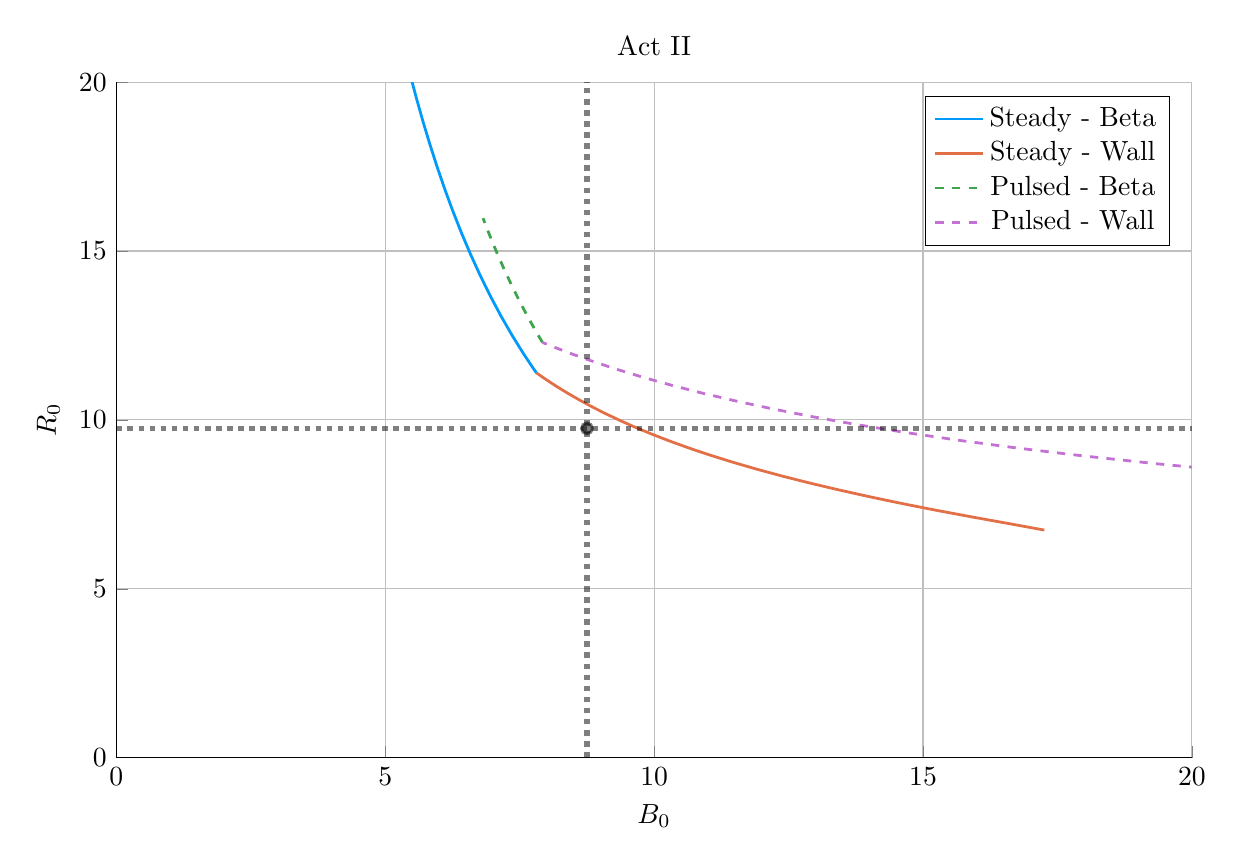
\begin{tikzpicture}[]
\begin{axis}[height = {101.6mm}, ylabel = {${R}_{0}$}, title = {Act II}, xmin = {0.0}, xmax = {20.0}, ymax = {20.0}, xlabel = {${B}_{0}$}, {unbounded coords=jump, scaled x ticks = false, xticklabel style={rotate = 0}, xmajorgrids = true, xtick = {0.0,5.0,10.0,15.0,20.0}, xticklabels = {0,5,10,15,20}, xtick align = inside, axis lines* = left, scaled y ticks = false, yticklabel style={rotate = 0}, ymajorgrids = true, ytick = {0.0,5.0,10.0,15.0,20.0}, yticklabels = {0,5,10,15,20}, ytick align = inside, axis lines* = left,     xshift = 0.0mm,
    yshift = 0.0mm,
    axis background/.style={fill={rgb,1:red,1.00000000;green,1.00000000;blue,1.00000000}}
, colorbar style={title=}}, ymin = {0.0}, width = {152.4mm}]\addplot+ [color = {rgb,1:red,0.00000000;green,0.60560316;blue,0.97868012},
draw opacity=1.0,
line width=1,
solid,mark = none,
mark size = 2.0,
mark options = {
    color = {rgb,1:red,0.00000000;green,0.00000000;blue,0.00000000}, draw opacity = 1.0,
    fill = {rgb,1:red,0.00000000;green,0.60560316;blue,0.97868012}, fill opacity = 1.0,
    line width = 1,
    rotate = 0,
    solid
}]coordinates {
(7.810935944285959, 11.389141268081966)
(7.57736049850867, 11.942634046586162)
(7.354864292609041, 12.51245847357923)
(7.145167234136329, 13.0943365692581)
(6.9473303865083675, 13.687993788149779)
(6.760499508614096, 14.293145886478186)
(6.583897990324067, 14.909495325365516)
(6.416817229618043, 15.536734694045393)
(6.258609820663305, 16.1745467994937)
(6.108683264880386, 16.82260538899235)
(5.966494431410919, 17.480575868750975)
(5.831544666176381, 18.148116014600475)
(5.703375459679132, 18.824876684423757)
(5.581564609582325, 19.510502502077443)
(5.465722802994068, 20.20463254880097)
(5.355490573482678, 20.906901035327614)
(5.25053558682053, 21.616937949657327)
(5.1505502068221745, 22.334369714080776)
(5.0552493196883175, 23.058819802110854)
};
\addlegendentry{Steady - Beta}
\addplot+ [color = {rgb,1:red,0.88887350;green,0.43564919;blue,0.27812294},
draw opacity=1.0,
line width=1,
solid,mark = none,
mark size = 2.0,
mark options = {
    color = {rgb,1:red,0.00000000;green,0.00000000;blue,0.00000000}, draw opacity = 1.0,
    fill = {rgb,1:red,0.88887350;green,0.43564919;blue,0.27812294}, fill opacity = 1.0,
    line width = 1,
    rotate = 0,
    solid
}]coordinates {
(17.25550839059296, 6.738604635617289)
(16.594334962335296, 6.931178286222189)
(15.9071755430688, 7.128187388035985)
(15.233983138507648, 7.327817939330552)
(14.594239858921854, 7.528927553154291)
(13.989673082630297, 7.7312042898700515)
(13.414782495717416, 7.934790159202381)
(12.872659546281994, 8.139273115071695)
(12.364365715508608, 8.344321605506495)
(11.889507953196574, 8.549679244077495)
(11.44685939646348, 8.755144058838903)
(11.034739998180656, 8.960554762148757)
(10.651252523287319, 9.165781242855727)
(10.294428800132035, 9.370717743724994)
(9.962319203963213, 9.57527782549947)
(9.653045819449929, 9.779390564591205)
(9.364832254395445, 9.982997628553138)
(9.096018465506306, 10.186050992034668)
(8.844373144802077, 10.388606525997883)
(8.61055754360846, 10.590345571972314)
(8.391192178573277, 10.791527736428888)
(8.18577947665566, 10.992035979756642)
(7.99323348423048, 11.1918525509058)
(7.812301489248497, 11.391007917726574)
};
\addlegendentry{Steady - Wall}
\addplot+ [color = {rgb,1:red,0.24222430;green,0.64327509;blue,0.30444865},
draw opacity=1.0,
line width=1,
dashed,mark = none,
mark size = 2.0,
mark options = {
    color = {rgb,1:red,0.00000000;green,0.00000000;blue,0.00000000}, draw opacity = 1.0,
    fill = {rgb,1:red,0.24222430;green,0.64327509;blue,0.30444865}, fill opacity = 1.0,
    line width = 1,
    rotate = 0,
    solid
}]coordinates {
(7.923668284887995, 12.293879059492616)
(7.923668284887995, 12.293879059492635)
(7.836759696043437, 12.52591633746021)
(7.6662731560983355, 13.00454403942661)
(7.50499428233835, 13.488375025456907)
(7.35232773269976, 13.977065733125242)
(7.207727224738343, 14.470269937628656)
(7.070690693175276, 14.967639476613451)
(6.940756001029682, 15.46882496625731)
(6.817497143644154, 15.973476480630131)
};
\addlegendentry{Pulsed - Beta}
\addplot+ [color = {rgb,1:red,0.76444018;green,0.44411178;blue,0.82429754},
draw opacity=1.0,
line width=1,
dashed,mark = none,
mark size = 2.0,
mark options = {
    color = {rgb,1:red,0.00000000;green,0.00000000;blue,0.00000000}, draw opacity = 1.0,
    fill = {rgb,1:red,0.76444018;green,0.44411178;blue,0.82429754}, fill opacity = 1.0,
    line width = 1,
    rotate = 0,
    solid
}]coordinates {
(22.56106430311702, 8.239911323116141)
(20.85607192394036, 8.471453471694678)
(19.335265246056654, 8.703260993170346)
(17.974121547130903, 8.935277031603567)
(16.751976718553127, 9.167446093344447)
(15.651329744019142, 9.399714010238458)
(14.65728744097675, 9.632027927077594)
(13.757118584462601, 9.864336290607328)
(12.939893642194303, 10.096588839007167)
(12.196191964860315, 10.328736591776112)
(11.517862472405039, 10.560731839999896)
(10.897827027335556, 10.792528137074703)
(10.329918077124672, 11.02408028901105)
(9.808743940706389, 11.255344346143936)
(9.329576544487265, 11.486277593626015)
(8.888257451278507, 11.716838542453242)
(8.481118883411932, 11.946986920205564)
(8.10491708701527, 12.17668366154026)
(7.923668284887995, 12.293879059492616)
(7.923668284887995, 12.293879059492635)
};
\addlegendentry{Pulsed - Wall}
\addplot+ [color = {rgb,1:red,0.00000000;green,0.00000000;blue,0.00000000},
draw opacity=0.5,
line width=2,
dotted,mark = none,
mark size = 2.0,
mark options = {
    color = {rgb,1:red,0.00000000;green,0.00000000;blue,0.00000000}, draw opacity = 0.5,
    fill = {rgb,1:red,0.00000000;green,0.00000000;blue,0.00000000}, fill opacity = 0.5,
    line width = 1,
    rotate = 0,
    solid
},forget plot]coordinates {
(0.0, 9.75)
(20.0, 9.75)
};
\addplot+ [color = {rgb,1:red,0.00000000;green,0.00000000;blue,0.00000000},
draw opacity=0.5,
line width=2,
dotted,mark = none,
mark size = 2.0,
mark options = {
    color = {rgb,1:red,0.00000000;green,0.00000000;blue,0.00000000}, draw opacity = 0.5,
    fill = {rgb,1:red,0.00000000;green,0.00000000;blue,0.00000000}, fill opacity = 0.5,
    line width = 1,
    rotate = 0,
    solid
},forget plot]coordinates {
(8.75, 0.0)
(8.75, 20.0)
};
\addplot+[draw=none, color = {rgb,1:red,0.00000000;green,0.00000000;blue,0.00000000},
draw opacity=0.5,
line width=0,
solid,mark = *,
mark size = 2.0,
mark options = {
    color = {rgb,1:red,0.00000000;green,0.00000000;blue,0.00000000}, draw opacity = 0.5,
    fill = {rgb,1:red,0.00000000;green,0.00000000;blue,0.00000000}, fill opacity = 0.5,
    line width = 1,
    rotate = 0,
    solid
},forget plot] coordinates {
(8.75, 9.75)
};
\end{axis}

\end{tikzpicture}

    \end{adjustbox}
        \caption{$R_0$ vs $B_0$}
    \end{subfigure}
    \hfill
    \begin{subfigure}[t]{0.45\textwidth}
        \centering
    \begin{adjustbox}{width=\textwidth}
      \Large
      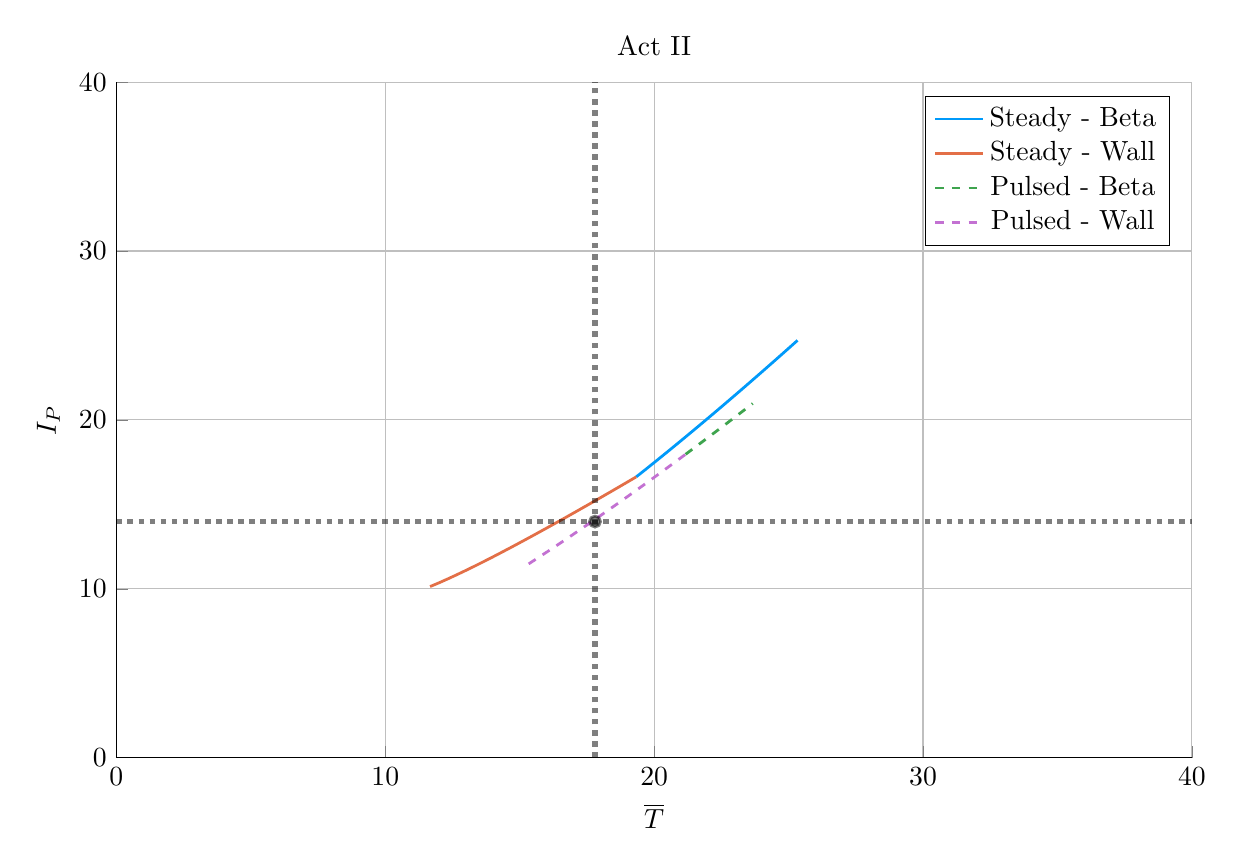
\begin{tikzpicture}[]
\begin{axis}[height = {101.6mm}, ylabel = {${I}_{P}$}, title = {Act II}, xmin = {0.0}, xmax = {40.0}, ymax = {40.0}, xlabel = {$\overline {T}$}, {unbounded coords=jump, scaled x ticks = false, xticklabel style={rotate = 0}, xmajorgrids = true, xtick = {0.0,10.0,20.0,30.0,40.0}, xticklabels = {0,10,20,30,40}, xtick align = inside, axis lines* = left, scaled y ticks = false, yticklabel style={rotate = 0}, ymajorgrids = true, ytick = {0.0,10.0,20.0,30.0,40.0}, yticklabels = {0,10,20,30,40}, ytick align = inside, axis lines* = left,     xshift = 0.0mm,
    yshift = 0.0mm,
    axis background/.style={fill={rgb,1:red,1.00000000;green,1.00000000;blue,1.00000000}}
, colorbar style={title=}}, ymin = {0.0}, width = {152.4mm}]\addplot+ [color = {rgb,1:red,0.00000000;green,0.60560316;blue,0.97868012},
draw opacity=1.0,
line width=1,
solid,mark = none,
mark size = 2.0,
mark options = {
    color = {rgb,1:red,0.00000000;green,0.00000000;blue,0.00000000}, draw opacity = 1.0,
    fill = {rgb,1:red,0.00000000;green,0.60560316;blue,0.97868012}, fill opacity = 1.0,
    line width = 1,
    rotate = 0,
    solid
}]coordinates {
(19.333333333333332, 16.626976584120992)
(19.666666666666668, 17.04714126565062)
(20.0, 17.4728205159228)
(20.333333333333332, 17.902037802268676)
(20.666666666666668, 18.334710756318135)
(21.0, 18.770758343299946)
(21.333333333333332, 19.21009903030823)
(21.666666666666668, 19.652652028291016)
(22.0, 20.098337062332053)
(22.333333333333332, 20.547074418426956)
(22.666666666666668, 20.998784986741654)
(23.0, 21.453390301179443)
(23.333333333333332, 21.910812577709113)
(23.666666666666668, 22.37097474604109)
(24.0, 22.833800482195542)
(24.333333333333332, 23.299214237115898)
(24.666666666666668, 23.767141260842724)
(25.0, 24.237507628970306)
(25.333333333333332, 24.710240262329886)
};
\addlegendentry{Steady - Beta}
\addplot+ [color = {rgb,1:red,0.88887350;green,0.43564919;blue,0.27812294},
draw opacity=1.0,
line width=1,
solid,mark = none,
mark size = 2.0,
mark options = {
    color = {rgb,1:red,0.00000000;green,0.00000000;blue,0.00000000}, draw opacity = 1.0,
    fill = {rgb,1:red,0.88887350;green,0.43564919;blue,0.27812294}, fill opacity = 1.0,
    line width = 1,
    rotate = 0,
    solid
}]coordinates {
(11.666666666666666, 10.131702672149428)
(12.0, 10.354462623384137)
(12.333333333333334, 10.591104956642406)
(12.666666666666666, 10.837356598740662)
(13.0, 11.09054386610192)
(13.333333333333334, 11.349883742416331)
(13.666666666666666, 11.61561327802365)
(14.0, 11.886764241828663)
(14.333333333333334, 12.16256217004895)
(14.666666666666666, 12.44240841774136)
(15.0, 12.72583049098312)
(15.333333333333334, 13.012449288635679)
(15.666666666666666, 13.301956539143166)
(16.0, 13.59409872387861)
(16.333333333333332, 13.888665310111481)
(16.666666666666668, 14.185479949266789)
(17.0, 14.48439377498311)
(17.333333333333332, 14.785280223642218)
(17.666666666666668, 15.088238807947413)
(18.0, 15.392552774473998)
(18.333333333333332, 15.698764813772398)
(18.666666666666668, 16.00659672680533)
(19.0, 16.315986303185774)
(19.333333333333332, 16.626976584120992)
};
\addlegendentry{Steady - Wall}
\addplot+ [color = {rgb,1:red,0.24222430;green,0.64327509;blue,0.30444865},
draw opacity=1.0,
line width=1,
dashed,mark = none,
mark size = 2.0,
mark options = {
    color = {rgb,1:red,0.00000000;green,0.00000000;blue,0.00000000}, draw opacity = 1.0,
    fill = {rgb,1:red,0.24222430;green,0.64327509;blue,0.30444865}, fill opacity = 1.0,
    line width = 1,
    rotate = 0,
    solid
}]coordinates {
(21.17034352159018, 17.96627417153032)
(21.170343521590212, 17.966274171530337)
(21.333333333333332, 18.1591936305205)
(21.666666666666668, 18.555297107283753)
(22.0, 18.953426399022014)
(22.333333333333332, 19.353497539767794)
(22.666666666666668, 19.7554274455778)
(23.0, 20.159133974954596)
(23.333333333333332, 20.564535986760628)
(23.666666666666668, 20.971553389451927)
};
\addlegendentry{Pulsed - Beta}
\addplot+ [color = {rgb,1:red,0.76444018;green,0.44411178;blue,0.82429754},
draw opacity=1.0,
line width=1,
dashed,mark = none,
mark size = 2.0,
mark options = {
    color = {rgb,1:red,0.00000000;green,0.00000000;blue,0.00000000}, draw opacity = 1.0,
    fill = {rgb,1:red,0.76444018;green,0.44411178;blue,0.82429754}, fill opacity = 1.0,
    line width = 1,
    rotate = 0,
    solid
}]coordinates {
(15.333333333333334, 11.474678053719876)
(15.666666666666666, 11.819475032994422)
(16.0, 12.167858357397087)
(16.333333333333332, 12.51974460671026)
(16.666666666666668, 12.875049128346197)
(17.0, 13.233686175102404)
(17.333333333333332, 13.595569077154208)
(17.666666666666668, 13.96061040317257)
(18.0, 14.328722110173729)
(18.333333333333332, 14.699815683529526)
(18.666666666666668, 15.073802268415148)
(19.0, 15.450592793824576)
(19.333333333333332, 15.830098089115069)
(19.666666666666668, 16.21222899561205)
(20.0, 16.596896471191773)
(20.333333333333332, 16.984011690059134)
(20.666666666666668, 17.37348613728185)
(21.0, 17.765231698435688)
(21.17034352159018, 17.96627417153032)
(21.170343521590212, 17.966274171530337)
};
\addlegendentry{Pulsed - Wall}
\addplot+ [color = {rgb,1:red,0.00000000;green,0.00000000;blue,0.00000000},
draw opacity=0.5,
line width=2,
dotted,mark = none,
mark size = 2.0,
mark options = {
    color = {rgb,1:red,0.00000000;green,0.00000000;blue,0.00000000}, draw opacity = 0.5,
    fill = {rgb,1:red,0.00000000;green,0.00000000;blue,0.00000000}, fill opacity = 0.5,
    line width = 1,
    rotate = 0,
    solid
},forget plot]coordinates {
(0.0, 13.98)
(40.0, 13.98)
};
\addplot+ [color = {rgb,1:red,0.00000000;green,0.00000000;blue,0.00000000},
draw opacity=0.5,
line width=2,
dotted,mark = none,
mark size = 2.0,
mark options = {
    color = {rgb,1:red,0.00000000;green,0.00000000;blue,0.00000000}, draw opacity = 0.5,
    fill = {rgb,1:red,0.00000000;green,0.00000000;blue,0.00000000}, fill opacity = 0.5,
    line width = 1,
    rotate = 0,
    solid
},forget plot]coordinates {
(17.8, 0.0)
(17.8, 40.0)
};
\addplot+[draw=none, color = {rgb,1:red,0.00000000;green,0.00000000;blue,0.00000000},
draw opacity=0.5,
line width=0,
solid,mark = *,
mark size = 2.0,
mark options = {
    color = {rgb,1:red,0.00000000;green,0.00000000;blue,0.00000000}, draw opacity = 0.5,
    fill = {rgb,1:red,0.00000000;green,0.00000000;blue,0.00000000}, fill opacity = 0.5,
    line width = 1,
    rotate = 0,
    solid
},forget plot] coordinates {
(17.8, 13.98)
};
\end{axis}

\end{tikzpicture}

    \end{adjustbox}
        \caption{$I_P$ vs $\overline T$}
    \end{subfigure}
    \hfill \hfill ~\\ ~\\ ~\\
    \caption{Aries Act II Model Comparison} ~\\
\end{figure*}

\begin{table}[h!]
\centering  
\caption{Act II Variables}
\hfill
\begin{subtable}[t]{0.4\textwidth}
\centering  
\caption{Input Variables} ~\\
\begin{tabular}{ c|c } 

Input            & Value           \\
\hline
$H$              & 1.22            \\
$Q$              & 25.0            \\
$N_{G}$          & 1.3             \\
$\epsilon$       & 0.25            \\
$\kappa_{95}$    & 1.964           \\
$\delta_{95}$    & 0.42            \\
$\nu_{n}$        & 0.41            \\
$\nu_{T}$        & 1.15            \\
$l_{i}$          & 0.60275         \\
$A$              & 2.5             \\
$Z_{eff}$        & 2.12            \\
$f_{D}$          & 0.74            \\
$\tau_{FT}$      & 1.6e9           \\
$B_{CS}$         & 12.77           \\

\end{tabular}
\end{subtable}
\hfill
\begin{subtable}[t]{0.5\textwidth}
\centering  
\caption{Output Variables} ~\\
\begin{tabular}{ c|c|c } 

Output           & Original         & Fussy.jl        \\
\hline
$R_{0}$          & 9.75             & 10.22           \\
$B_{0}$          & 8.75             & 9.05           \\
$I_{P}$          & 13.98            & 14.84           \\
$\overline n$    & 0.86             & 0.82          \\
$\overline T$    & 17.8             & 17.4           \\
$\beta_{N}$       & 0.026            & 0.023          \\
$q_{95}$         & 8.0              & 6.6           \\
$P_{W}$          & 1.46             & -            \\
$f_{BS}$         & 0.77             & 0.66           \\
$f_{CD}$         & 0.23             & 0.34           \\
$f_{IN}$         & -              & -             \\
$\volume$         & 2209           & 2559          \\
$P_{F}$          & 2637           & 3460          \\
$\eta_{CD}$      & 0.256            & 0.307           \\

\end{tabular}
\end{subtable}
\hfill
\hfill
\end{table}

\newpage

\subsection{Benchmarking with the Process DEMO Designs}

The PROCESS team's prospective designs for successors to ITER constitute the final set of model comparisons: the steady-state and pulsed DEMO reactors. As this paper is designed to compare these modes of operation, this study proves most fruitful. It also highlights how common model decisions can dramatically alter what reactors come out of the solvers.

The first discrepancy is how the PROCESS team defines the loss term in the ELMy H-Mode scaling law. As shown in their paper, they actually subtract out a Bremsstrahlung component, while leaving the fitting coefficients the same. \cite{process} After modifying Fussy.jl to incorporate this definition, the steady-state reactor is easily reproducible in $R_0$ -- $B_0$ slice of reactor space.

Unlike the steady-state cause, however, the modified power loss term does not fix the pulsed case, as it actually draws the reactor curves further from the design from their paper. As such, it is flux balance that is now the main source of discrepancy between the two models. This makes sense, as this model uses highly simplified source terms -- namely neglecting anything but the central solenoid and PF coils (as well as ignoring crucial physics for these two components).

Even acknowledging the differences between the two models, Fussy.jl still does remarkably well at reproducing their much more sophisticated coding framework. The final point to make is about selecting optimum points to build as the floating variables are allowed to make curves through reactor space. Up to this point, only steady-state tokamak designs have been explored. In every single one of these, the paper values have been very close to the point where the beta curves and wall loading curves cross. This is because they all result in the minimum cost-per-watt. 

For pulsed designs, on the other hand, kink curves start to appear for low magnetic field strengths. Just as beta-wall intersections were optimum places to design for low cost-per-watt ($C_W$) reactors, these beta-kink intersections will prove to be the place where minimum capital cost ($W_M$) reactors usually occur.

\newpage 

\subsubsection{DEMO Steady -- A Steady-State ITER Successor}

Hands down, this DEMO Steady reactor is the worst modeled reactor using Fussy.jl. As mentioned previously, though, some of the discrepancy was removed by using the PROCESS team's modified version of heat loss. This heavily corrected the $R_0$ -- $B_0$ curve, but had no effect on the $I_P$ -- $\overline T$ one. An interesting aside, these curves actually show that the steady current is independent of secondary constraint (as discussed).

\begin{figure*}[h!]
    \centering
    \hfill 
    \begin{subfigure}[t]{0.45\textwidth}
        \centering
    \begin{adjustbox}{width=\textwidth}
      \Large
      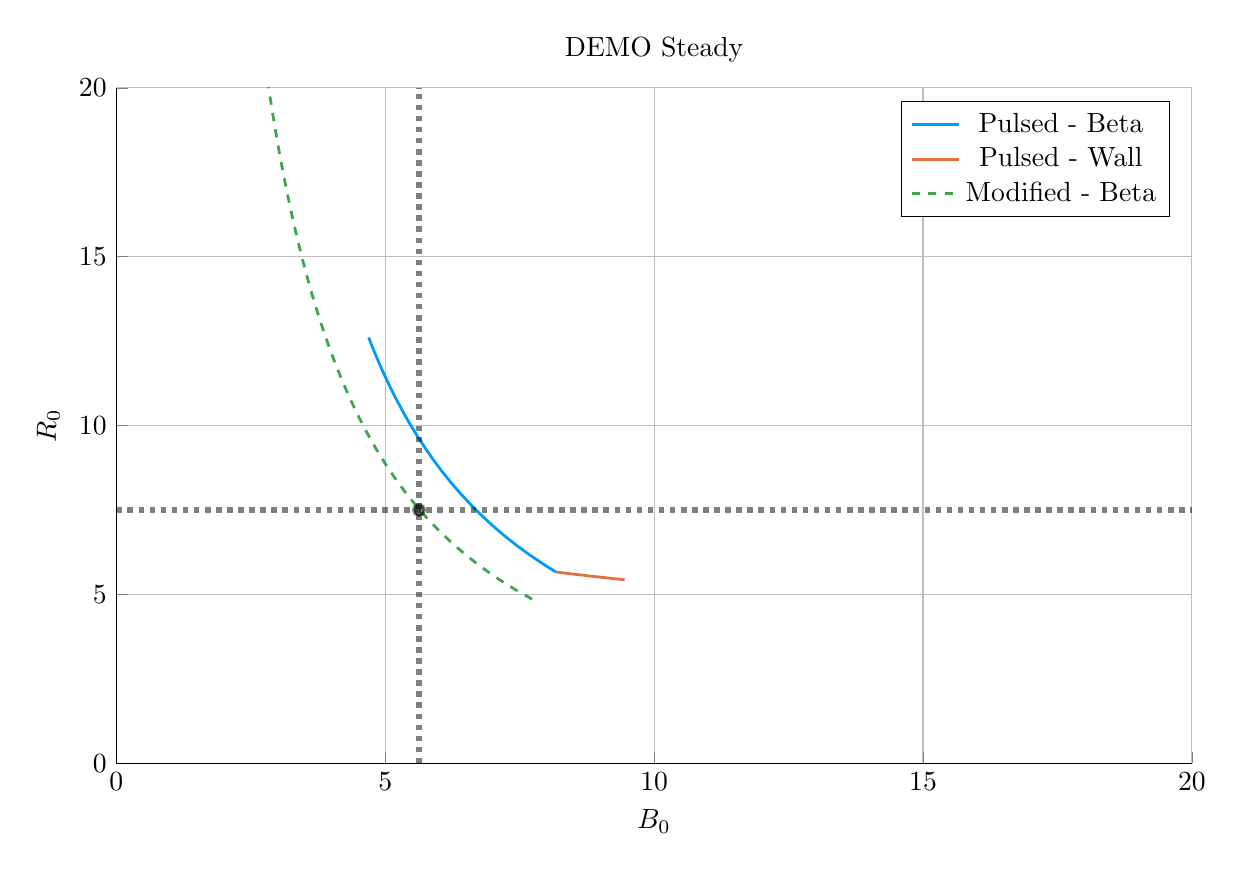
\begin{tikzpicture}[]
\begin{axis}[height = {101.6mm}, ylabel = {${R}_{0}$}, title = {DEMO Steady}, xmin = {0.0}, xmax = {20.0}, ymax = {20.0}, xlabel = {${B}_{0}$}, {unbounded coords=jump, scaled x ticks = false, xticklabel style={rotate = 0}, xmajorgrids = true, xtick = {0.0,5.0,10.0,15.0,20.0}, xticklabels = {0,5,10,15,20}, xtick align = inside, axis lines* = left, scaled y ticks = false, yticklabel style={rotate = 0}, ymajorgrids = true, ytick = {0.0,5.0,10.0,15.0,20.0}, yticklabels = {0,5,10,15,20}, ytick align = inside, axis lines* = left,     xshift = 0.0mm,
    yshift = 0.0mm,
    axis background/.style={fill={rgb,1:red,1.00000000;green,1.00000000;blue,1.00000000}}
, colorbar style={title=}}, ymin = {0.0}, width = {152.4mm}]\addplot+ [color = {rgb,1:red,0.00000000;green,0.60560316;blue,0.97868012},
draw opacity=1.0,
line width=1,
solid,mark = none,
mark size = 2.0,
mark options = {
    color = {rgb,1:red,0.00000000;green,0.00000000;blue,0.00000000}, draw opacity = 1.0,
    fill = {rgb,1:red,0.00000000;green,0.60560316;blue,0.97868012}, fill opacity = 1.0,
    line width = 1,
    rotate = 0,
    solid
}]coordinates {
(8.173486873088942, 5.664794455960266)
(7.942780080136996, 5.894389477908349)
(7.682110747013332, 6.174587309854596)
(7.436076373351653, 6.4617259587740365)
(7.203701032854224, 6.7556817964635885)
(6.984087846006315, 7.056316762210614)
(6.776411507024863, 7.363478485110443)
(6.579911624110169, 7.677000456183209)
(6.393886772782909, 7.996702249919802)
(6.217689175869905, 8.322389794615686)
(6.050719935402341, 8.653855690575247)
(5.892424751644716, 8.990879574996331)
(5.742290072962272, 9.333228532083597)
(5.599839627496144, 9.680657546690735)
(5.464631293842628, 10.03290999955685)
(5.33625427328881, 10.389718201981736)
(5.214326530771975, 10.75080396758328)
(5.098492475718857, 11.115879218594692)
(4.98842085737482, 11.484646623994054)
(4.88380285223036, 11.85680026661456)
(4.784350323760147, 12.232026336259217)
(4.689794236961777, 12.610003845742904)
};
\addlegendentry{Pulsed - Beta}
\addplot+ [color = {rgb,1:red,0.88887350;green,0.43564919;blue,0.27812294},
draw opacity=1.0,
line width=1,
solid,mark = none,
mark size = 2.0,
mark options = {
    color = {rgb,1:red,0.00000000;green,0.00000000;blue,0.00000000}, draw opacity = 1.0,
    fill = {rgb,1:red,0.88887350;green,0.43564919;blue,0.27812294}, fill opacity = 1.0,
    line width = 1,
    rotate = 0,
    solid
}]coordinates {
(9.452194760190558, 5.436039445052516)
(8.82895875946862, 5.541751345019407)
(8.260410483462291, 5.64769543408014)
(8.173486873088942, 5.664794455960266)
};
\addlegendentry{Pulsed - Wall}
\addplot+ [color = {rgb,1:red,0.24222430;green,0.64327509;blue,0.30444865},
draw opacity=1.0,
line width=1,
dashed,mark = none,
mark size = 2.0,
mark options = {
    color = {rgb,1:red,0.00000000;green,0.00000000;blue,0.00000000}, draw opacity = 1.0,
    fill = {rgb,1:red,0.24222430;green,0.64327509;blue,0.30444865}, fill opacity = 1.0,
    line width = 1,
    rotate = 0,
    solid
}]coordinates {
(7.729015258613306, 4.861871150043874)
(7.398090906424027, 5.162615732748398)
(7.087604971989989, 5.475689582149146)
(6.796029845186129, 5.801261884855786)
(6.5219747916377235, 6.139486028413868)
(6.264171517105504, 6.490498735804173)
(6.021461495247516, 6.854419238072999)
(5.792784817023639, 7.231348485954994)
(5.57717035299729, 7.621368405021026)
(5.3737270519036775, 8.024541198865679)
(5.1816362256187425, 8.440908704652248)
(5.000144692923053, 8.870491805097014)
(4.828558673035444, 9.313289900712723)
(4.666238335465348, 9.769280445839089)
(4.512592925835539, 10.23841855166636)
(4.367076398389423, 10.720636659108127)
(4.229183495269078, 11.215844284001262)
(4.098446220614958, 11.723927836706606)
(3.974430664327246, 12.244750517759236)
(3.856734136133517, 12.778152290770123)
(3.744982575583214, 13.323949933321568)
(3.6388282078672565, 13.881937166125676)
(3.537947419047361, 14.45188486023713)
(3.4420388274654035, 15.033541321628862)
(3.3508215308612357, 15.626632651963563)
(3.2640335111230074, 16.230863183919308)
(3.18143018067718, 16.84591598897328)
(3.1027830563428513, 17.471453455103656)
(3.0278785480626333, 18.107117931452404)
(2.956516851312625, 18.752532436599008)
(2.888510933213844, 19.407301426734122)
(2.823685603439882, 20.071011619694055)
(2.761876661959762, 20.74323287052923)
(2.702930116488407, 21.423519094029906)
(2.646701463253573, 22.111409229427537)
(2.593055025340143, 22.806428242329144)
};
\addlegendentry{Modified - Beta}
\addplot+ [color = {rgb,1:red,0.00000000;green,0.00000000;blue,0.00000000},
draw opacity=0.5,
line width=2,
dotted,mark = none,
mark size = 2.0,
mark options = {
    color = {rgb,1:red,0.00000000;green,0.00000000;blue,0.00000000}, draw opacity = 0.5,
    fill = {rgb,1:red,0.00000000;green,0.00000000;blue,0.00000000}, fill opacity = 0.5,
    line width = 1,
    rotate = 0,
    solid
},forget plot]coordinates {
(0.0, 7.5)
(20.0, 7.5)
};
\addplot+ [color = {rgb,1:red,0.00000000;green,0.00000000;blue,0.00000000},
draw opacity=0.5,
line width=2,
dotted,mark = none,
mark size = 2.0,
mark options = {
    color = {rgb,1:red,0.00000000;green,0.00000000;blue,0.00000000}, draw opacity = 0.5,
    fill = {rgb,1:red,0.00000000;green,0.00000000;blue,0.00000000}, fill opacity = 0.5,
    line width = 1,
    rotate = 0,
    solid
},forget plot]coordinates {
(5.627, 0.0)
(5.627, 20.0)
};
\addplot+[draw=none, color = {rgb,1:red,0.00000000;green,0.00000000;blue,0.00000000},
draw opacity=0.5,
line width=0,
solid,mark = *,
mark size = 2.0,
mark options = {
    color = {rgb,1:red,0.00000000;green,0.00000000;blue,0.00000000}, draw opacity = 0.5,
    fill = {rgb,1:red,0.00000000;green,0.00000000;blue,0.00000000}, fill opacity = 0.5,
    line width = 1,
    rotate = 0,
    solid
},forget plot] coordinates {
(5.627, 7.5)
};
\end{axis}

\end{tikzpicture}

    \end{adjustbox}
        \caption{$R_0$ vs $B_0$}
    \end{subfigure}
    \hfill
    \begin{subfigure}[t]{0.45\textwidth}
        \centering
    \begin{adjustbox}{width=\textwidth}
      \Large
      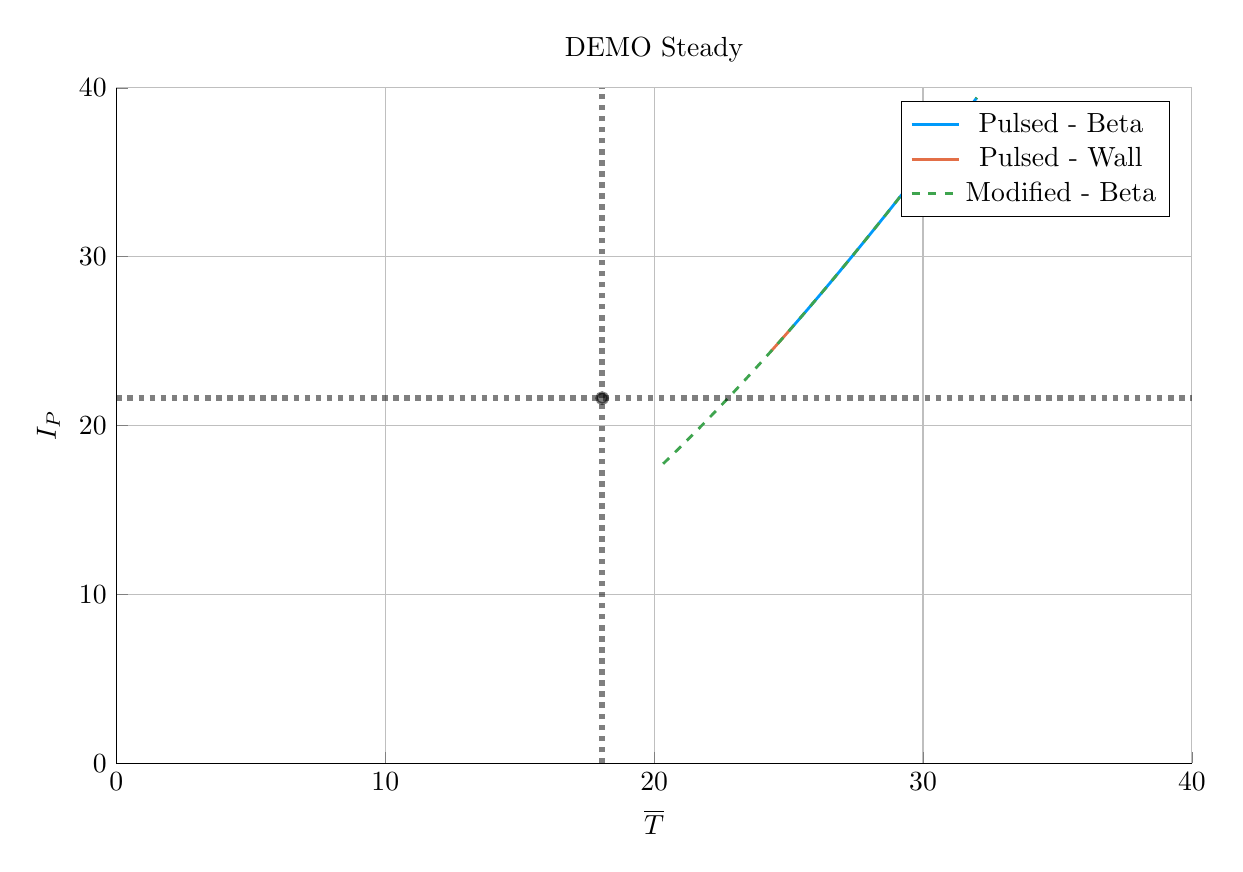
\begin{tikzpicture}[]
\begin{axis}[height = {101.6mm}, ylabel = {${I}_{P}$}, title = {DEMO Steady}, xmin = {0.0}, xmax = {40.0}, ymax = {40.0}, xlabel = {$\overline {T}$}, {unbounded coords=jump, scaled x ticks = false, xticklabel style={rotate = 0}, xmajorgrids = true, xtick = {0.0,10.0,20.0,30.0,40.0}, xticklabels = {0,10,20,30,40}, xtick align = inside, axis lines* = left, scaled y ticks = false, yticklabel style={rotate = 0}, ymajorgrids = true, ytick = {0.0,10.0,20.0,30.0,40.0}, yticklabels = {0,10,20,30,40}, ytick align = inside, axis lines* = left,     xshift = 0.0mm,
    yshift = 0.0mm,
    axis background/.style={fill={rgb,1:red,1.00000000;green,1.00000000;blue,1.00000000}}
, colorbar style={title=}}, ymin = {0.0}, width = {152.4mm}]\addplot+ [color = {rgb,1:red,0.00000000;green,0.60560316;blue,0.97868012},
draw opacity=1.0,
line width=1,
solid,mark = none,
mark size = 2.0,
mark options = {
    color = {rgb,1:red,0.00000000;green,0.00000000;blue,0.00000000}, draw opacity = 1.0,
    fill = {rgb,1:red,0.00000000;green,0.60560316;blue,0.97868012}, fill opacity = 1.0,
    line width = 1,
    rotate = 0,
    solid
}]coordinates {
(25.053735982163357, 25.677558860299992)
(25.333333333333332, 26.189593064380034)
(25.666666666666668, 26.80548085953921)
(26.0, 27.427148406840605)
(26.333333333333332, 28.054440831282633)
(26.666666666666668, 28.68719962041386)
(27.0, 29.325262818659787)
(27.333333333333332, 29.968465226287904)
(27.666666666666668, 30.6166386025962)
(28.0, 31.269611872884024)
(28.333333333333332, 31.92721133872904)
(28.666666666666668, 32.589260891064264)
(29.0, 33.25558222552837)
(29.333333333333332, 33.925995059549685)
(29.666666666666668, 34.60031735061725)
(30.0, 35.27836551518855)
(30.333333333333332, 35.95995464768734)
(30.666666666666668, 36.644898739049395)
(31.0, 37.333010894283476)
(31.333333333333332, 38.02410354852819)
(31.666666666666668, 38.717988681099214)
(32.0, 39.41447802704077)
};
\addlegendentry{Pulsed - Beta}
\addplot+ [color = {rgb,1:red,0.88887350;green,0.43564919;blue,0.27812294},
draw opacity=1.0,
line width=1,
solid,mark = none,
mark size = 2.0,
mark options = {
    color = {rgb,1:red,0.00000000;green,0.00000000;blue,0.00000000}, draw opacity = 1.0,
    fill = {rgb,1:red,0.88887350;green,0.43564919;blue,0.27812294}, fill opacity = 1.0,
    line width = 1,
    rotate = 0,
    solid
}]coordinates {
(24.333333333333332, 24.378107374495485)
(24.666666666666668, 24.975762903314084)
(25.0, 25.579637086786484)
(25.053735982163357, 25.677558860299992)
};
\addlegendentry{Pulsed - Wall}
\addplot+ [color = {rgb,1:red,0.24222430;green,0.64327509;blue,0.30444865},
draw opacity=1.0,
line width=1,
dashed,mark = none,
mark size = 2.0,
mark options = {
    color = {rgb,1:red,0.00000000;green,0.00000000;blue,0.00000000}, draw opacity = 1.0,
    fill = {rgb,1:red,0.24222430;green,0.64327509;blue,0.30444865}, fill opacity = 1.0,
    line width = 1,
    rotate = 0,
    solid
}]coordinates {
(20.333333333333332, 17.737142606162497)
(20.666666666666668, 18.250736761644205)
(21.0, 18.771889258341997)
(21.333333333333332, 19.300518519223587)
(21.666666666666668, 19.836537357082282)
(22.0, 20.37985305559639)
(22.333333333333332, 20.930367463801495)
(22.666666666666668, 21.487977099646507)
(23.0, 22.05257326267931)
(23.333333333333332, 22.62404215595106)
(23.666666666666668, 23.202265017123075)
(24.0, 23.787118258664318)
(24.333333333333332, 24.378473616949)
(24.666666666666668, 24.976198309995638)
(25.0, 25.58015520352756)
(25.333333333333332, 26.19020298497985)
(25.666666666666668, 26.806196345025047)
(26.0, 27.427986166140983)
(26.333333333333332, 28.055419717698932)
(26.666666666666668, 28.688340857006587)
(27.0, 29.3265902357016)
(27.333333333333332, 29.970005510854897)
(27.666666666666668, 30.61842156011136)
(28.0, 31.27167070016686)
(28.333333333333332, 31.92958290785876)
(28.666666666666668, 32.591986043126525)
(29.0, 33.25870607308836)
(29.333333333333332, 33.929567296470175)
(29.666666666666668, 34.604392567622554)
(30.0, 35.28300351936469)
(30.333333333333332, 35.96522078390488)
(30.666666666666668, 36.650864211102025)
(31.0, 37.3397530833557)
(31.333333333333332, 38.03170632643894)
(31.666666666666668, 38.726542715621264)
(32.0, 39.424081076468326)
};
\addlegendentry{Modified - Beta}
\addplot+ [color = {rgb,1:red,0.00000000;green,0.00000000;blue,0.00000000},
draw opacity=0.5,
line width=2,
dotted,mark = none,
mark size = 2.0,
mark options = {
    color = {rgb,1:red,0.00000000;green,0.00000000;blue,0.00000000}, draw opacity = 0.5,
    fill = {rgb,1:red,0.00000000;green,0.00000000;blue,0.00000000}, fill opacity = 0.5,
    line width = 1,
    rotate = 0,
    solid
},forget plot]coordinates {
(0.0, 21.627)
(40.0, 21.627)
};
\addplot+ [color = {rgb,1:red,0.00000000;green,0.00000000;blue,0.00000000},
draw opacity=0.5,
line width=2,
dotted,mark = none,
mark size = 2.0,
mark options = {
    color = {rgb,1:red,0.00000000;green,0.00000000;blue,0.00000000}, draw opacity = 0.5,
    fill = {rgb,1:red,0.00000000;green,0.00000000;blue,0.00000000}, fill opacity = 0.5,
    line width = 1,
    rotate = 0,
    solid
},forget plot]coordinates {
(18.067, 0.0)
(18.067, 40.0)
};
\addplot+[draw=none, color = {rgb,1:red,0.00000000;green,0.00000000;blue,0.00000000},
draw opacity=0.5,
line width=0,
solid,mark = *,
mark size = 2.0,
mark options = {
    color = {rgb,1:red,0.00000000;green,0.00000000;blue,0.00000000}, draw opacity = 0.5,
    fill = {rgb,1:red,0.00000000;green,0.00000000;blue,0.00000000}, fill opacity = 0.5,
    line width = 1,
    rotate = 0,
    solid
},forget plot] coordinates {
(18.067, 21.627)
};
\end{axis}

\end{tikzpicture}

    \end{adjustbox}
        \caption{$I_P$ vs $\overline T$}
    \end{subfigure}
    \hfill \hfill ~\\ ~\\ ~\\
    \caption{Demo Steady Model Comparison} ~\\
\end{figure*}

\begin{table}[h!]
\centering  
\caption{Demo Steady Variables}
\hfill
\begin{subtable}[t]{0.4\textwidth}
\centering  
\caption{Input Variables} ~\\
\begin{tabular}{ c|c } 

Input            & Value           \\
\hline
$H$              & 1.4             \\
$Q$              & 24.46           \\
$N_{G}$          & 1.2             \\
$\epsilon$       & 0.385           \\
$\kappa_{95}$    & 1.8             \\
$\delta_{95}$    & 0.333           \\
$\nu_{n}$        & 0.3972          \\
$\nu_{T}$        & 0.9187          \\
$l_{i}$          & 0.9             \\
$A$              & 2.856           \\
$Z_{eff}$        & 4.708           \\
$f_{D}$          & 0.7366          \\
$\tau_{FT}$      & 1.6e9           \\
$B_{CS}$         & 12.85           \\

\end{tabular}
\end{subtable}
\hfill
\begin{subtable}[t]{0.5\textwidth}
\centering  
\caption{Output Variables} ~\\
\begin{tabular}{ c|c|c } 

Output           & Original         & Fussy.jl        \\  
\hline
$R_{0}$          & 7.5              & 8.2           \\
$B_{0}$          & 5.627            & 6.307           \\
$I_{P}$          & 21.63            & 30.93           \\
$\overline n$    & 0.8746           & 1.048           \\
$\overline T$    & 18.07            & 27.83           \\
$\beta_{N}$       & 0.038            & -           \\
$q_{95}$         & 4.405            & 3.761           \\
$P_{W}$          & 1.911            & 4.151           \\
$f_{BS}$         & 0.611            & 0.424          \\
$f_{CD}$         & 0.389            & 0.576          \\
$f_{IN}$         & -              & -             \\
$\volume$         & 2217           & 2879          \\
$P_{F}$          & 3255           & 8971          \\
$\eta_{CD}$      & 0.4152           & -          \\

\end{tabular}
\end{subtable}
\hfill
\hfill
\end{table}

\newpage 

\subsubsection{DEMO Pulsed -- A Pulsed ITER Successor}

This pulsed version of DEMO is the only reactor in our collection that is not run in steady-state. As such, it may be the most important one. The first thing that is abundantly clear is that this design actually has no valid wall loading portion -- only a kink and beta curve exist! Even so, the results match pretty well. It should be noted, though, that this current drive is treated as an input and not solved self-consistently.

\begin{figure*}[h!]
    \centering
    \hfill 
    \begin{subfigure}[t]{0.45\textwidth}
        \centering
    \begin{adjustbox}{width=\textwidth}
      \Large
      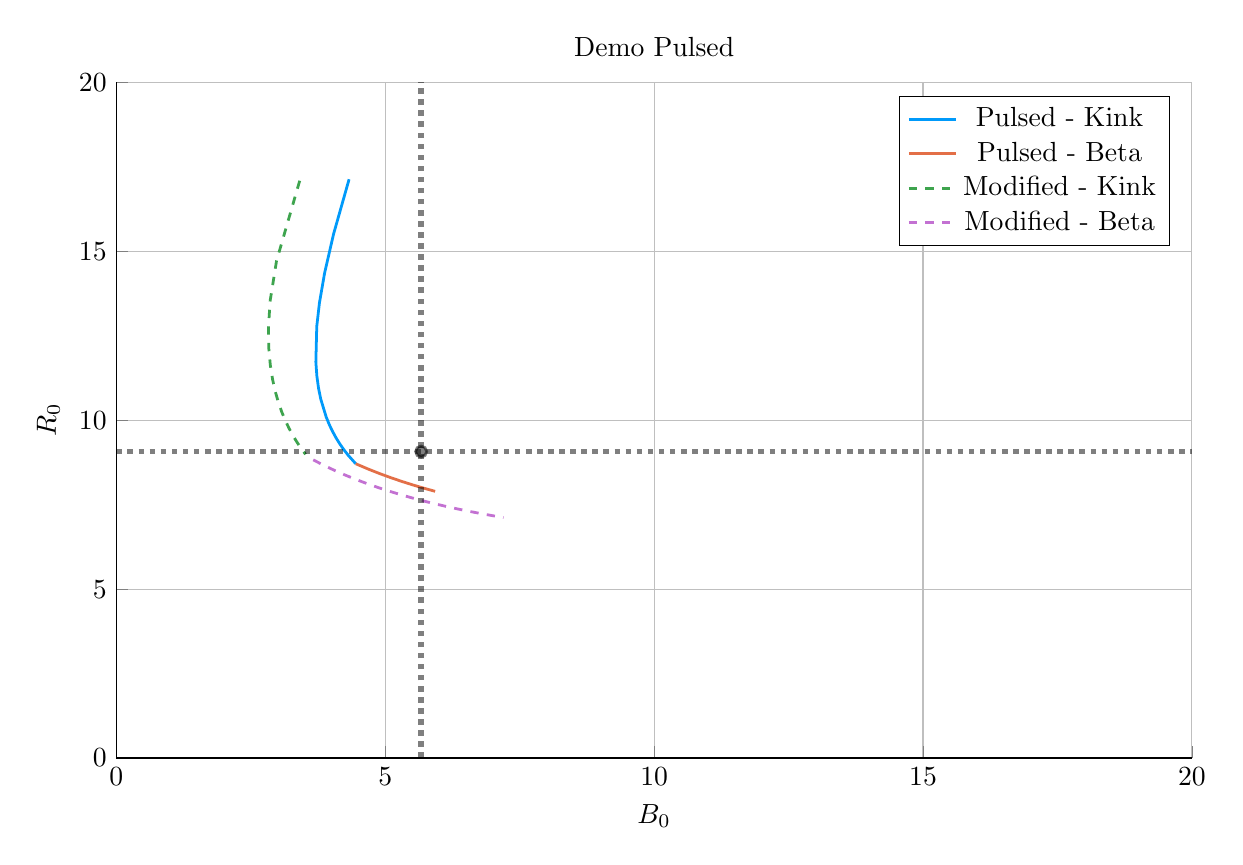
\begin{tikzpicture}[]
\begin{axis}[height = {101.6mm}, ylabel = {${R}_{0}$}, title = {Demo Pulsed}, xmin = {0.0}, xmax = {20.0}, ymax = {20.0}, xlabel = {${B}_{0}$}, {unbounded coords=jump, scaled x ticks = false, xticklabel style={rotate = 0}, xmajorgrids = true, xtick = {0.0,5.0,10.0,15.0,20.0}, xticklabels = {0,5,10,15,20}, xtick align = inside, axis lines* = left, scaled y ticks = false, yticklabel style={rotate = 0}, ymajorgrids = true, ytick = {0.0,5.0,10.0,15.0,20.0}, yticklabels = {0,5,10,15,20}, ytick align = inside, axis lines* = left,     xshift = 0.0mm,
    yshift = 0.0mm,
    axis background/.style={fill={rgb,1:red,1.00000000;green,1.00000000;blue,1.00000000}}
, colorbar style={title=}}, ymin = {0.0}, width = {152.4mm}]\addplot+ [color = {rgb,1:red,0.00000000;green,0.60560316;blue,0.97868012},
draw opacity=1.0,
line width=1,
solid,mark = none,
mark size = 2.0,
mark options = {
    color = {rgb,1:red,0.00000000;green,0.00000000;blue,0.00000000}, draw opacity = 1.0,
    fill = {rgb,1:red,0.00000000;green,0.60560316;blue,0.97868012}, fill opacity = 1.0,
    line width = 1,
    rotate = 0,
    solid
}]coordinates {
(4.327031075670194, 17.134796748649162)
(4.038214026054326, 15.511755022601415)
(3.8713719163129245, 14.355562963913712)
(3.7758613845615545, 13.476675762289453)
(3.7257856761317214, 12.778294295391971)
(3.7090473695925437, 11.723065749829066)
(3.727711597554826, 11.30970201784727)
(3.7586131667481433, 10.94971275897184)
(3.799052518631718, 10.632190690377048)
(3.901290136389271, 10.09455415135144)
(3.960577465316514, 9.863813619410237)
(4.0241209645210345, 9.653307397969705)
(4.0912717805663785, 9.460162902699798)
(4.161514602943343, 9.28206292757184)
(4.2344343960723005, 9.117114543572253)
(4.309692554546368, 8.963753917462126)
(4.450417240491067, 8.712493965092264)
};
\addlegendentry{Pulsed - Kink}
\addplot+ [color = {rgb,1:red,0.88887350;green,0.43564919;blue,0.27812294},
draw opacity=1.0,
line width=1,
solid,mark = none,
mark size = 2.0,
mark options = {
    color = {rgb,1:red,0.00000000;green,0.00000000;blue,0.00000000}, draw opacity = 1.0,
    fill = {rgb,1:red,0.88887350;green,0.43564919;blue,0.27812294}, fill opacity = 1.0,
    line width = 1,
    rotate = 0,
    solid
}]coordinates {
(4.450417240491067, 8.712493965092264)
(4.490148631384312, 8.684308742646298)
(4.692490181445514, 8.547262773806349)
(4.8960344619053355, 8.41947837460442)
(5.100651132702229, 8.30014929484307)
(5.306202822090688, 8.188581738801314)
(5.512545696627038, 8.084175191078112)
(5.719530043226767, 7.986407002697611)
(5.927000883375481, 7.894819882619234)
};
\addlegendentry{Pulsed - Beta}
\addplot+ [color = {rgb,1:red,0.24222430;green,0.64327509;blue,0.30444865},
draw opacity=1.0,
line width=1,
dashed,mark = none,
mark size = 2.0,
mark options = {
    color = {rgb,1:red,0.00000000;green,0.00000000;blue,0.00000000}, draw opacity = 1.0,
    fill = {rgb,1:red,0.24222430;green,0.64327509;blue,0.30444865}, fill opacity = 1.0,
    line width = 1,
    rotate = 0,
    solid
}]coordinates {
(3.4087424183072135, 17.090884129081292)
(2.977074181068944, 14.713048632784332)
(2.8592500074202523, 13.541171522519205)
(2.827199220063259, 12.740024138753894)
(2.8339789008667826, 12.12574468151967)
(2.862412302880871, 11.626187613249266)
(2.9044598258085443, 11.205091848948229)
(2.95577893007882, 10.841432203317366)
(3.0137895352525907, 10.521822649209419)
(3.076849710218805, 10.23716073884787)
(3.1438583711612704, 9.980947801083442)
(3.214045733980633, 9.748367275345563)
(3.2868548955983727, 9.535742205343247)
(3.361871149981842, 9.340197658526863)
(3.4387778750377818, 9.15944098345979)
(3.5173279629378453, 8.991613349767409)
};
\addlegendentry{Modified - Kink}
\addplot+ [color = {rgb,1:red,0.76444018;green,0.44411178;blue,0.82429754},
draw opacity=1.0,
line width=1,
dashed,mark = none,
mark size = 2.0,
mark options = {
    color = {rgb,1:red,0.00000000;green,0.00000000;blue,0.00000000}, draw opacity = 1.0,
    fill = {rgb,1:red,0.76444018;green,0.44411178;blue,0.82429754}, fill opacity = 1.0,
    line width = 1,
    rotate = 0,
    solid
}]coordinates {
(3.6607028750648505, 8.825949645171955)
(3.8574448036470477, 8.664618827122876)
(4.056375867871351, 8.51434867582932)
(4.257366397480293, 8.374075613831488)
(4.460279103534801, 8.242896218794312)
(4.664969389370631, 8.12003771613466)
(4.871285596007394, 8.004834914067093)
(5.07906923307514, 7.896711937521184)
(5.288155233306219, 7.795167587687744)
(5.498372259673351, 7.699763475973523)
(5.709543087166185, 7.610114306522102)
(5.921485076209294, 7.525879840414137)
(6.134010749367255, 7.446758190646709)
(6.346928478632384, 7.372480180910637)
(6.560043285872518, 7.302804563889649)
(6.773157754368795, 7.237513941672651)
(6.986073044284746, 7.176411266758267)
(7.198590001107076, 7.119316828230052)
};
\addlegendentry{Modified - Beta}
\addplot+ [color = {rgb,1:red,0.00000000;green,0.00000000;blue,0.00000000},
draw opacity=0.5,
line width=2,
dotted,mark = none,
mark size = 2.0,
mark options = {
    color = {rgb,1:red,0.00000000;green,0.00000000;blue,0.00000000}, draw opacity = 0.5,
    fill = {rgb,1:red,0.00000000;green,0.00000000;blue,0.00000000}, fill opacity = 0.5,
    line width = 1,
    rotate = 0,
    solid
},forget plot]coordinates {
(0.0, 9.072)
(20.0, 9.072)
};
\addplot+ [color = {rgb,1:red,0.00000000;green,0.00000000;blue,0.00000000},
draw opacity=0.5,
line width=2,
dotted,mark = none,
mark size = 2.0,
mark options = {
    color = {rgb,1:red,0.00000000;green,0.00000000;blue,0.00000000}, draw opacity = 0.5,
    fill = {rgb,1:red,0.00000000;green,0.00000000;blue,0.00000000}, fill opacity = 0.5,
    line width = 1,
    rotate = 0,
    solid
},forget plot]coordinates {
(5.667, 0.0)
(5.667, 20.0)
};
\addplot+[draw=none, color = {rgb,1:red,0.00000000;green,0.00000000;blue,0.00000000},
draw opacity=0.5,
line width=0,
solid,mark = *,
mark size = 2.0,
mark options = {
    color = {rgb,1:red,0.00000000;green,0.00000000;blue,0.00000000}, draw opacity = 0.5,
    fill = {rgb,1:red,0.00000000;green,0.00000000;blue,0.00000000}, fill opacity = 0.5,
    line width = 1,
    rotate = 0,
    solid
},forget plot] coordinates {
(5.667, 9.072)
};
\end{axis}

\end{tikzpicture}

    \end{adjustbox}
        \caption{$R_0$ vs $B_0$}
    \end{subfigure}
    \hfill
    \begin{subfigure}[t]{0.45\textwidth}
        \centering
    \begin{adjustbox}{width=\textwidth}
      \Large
      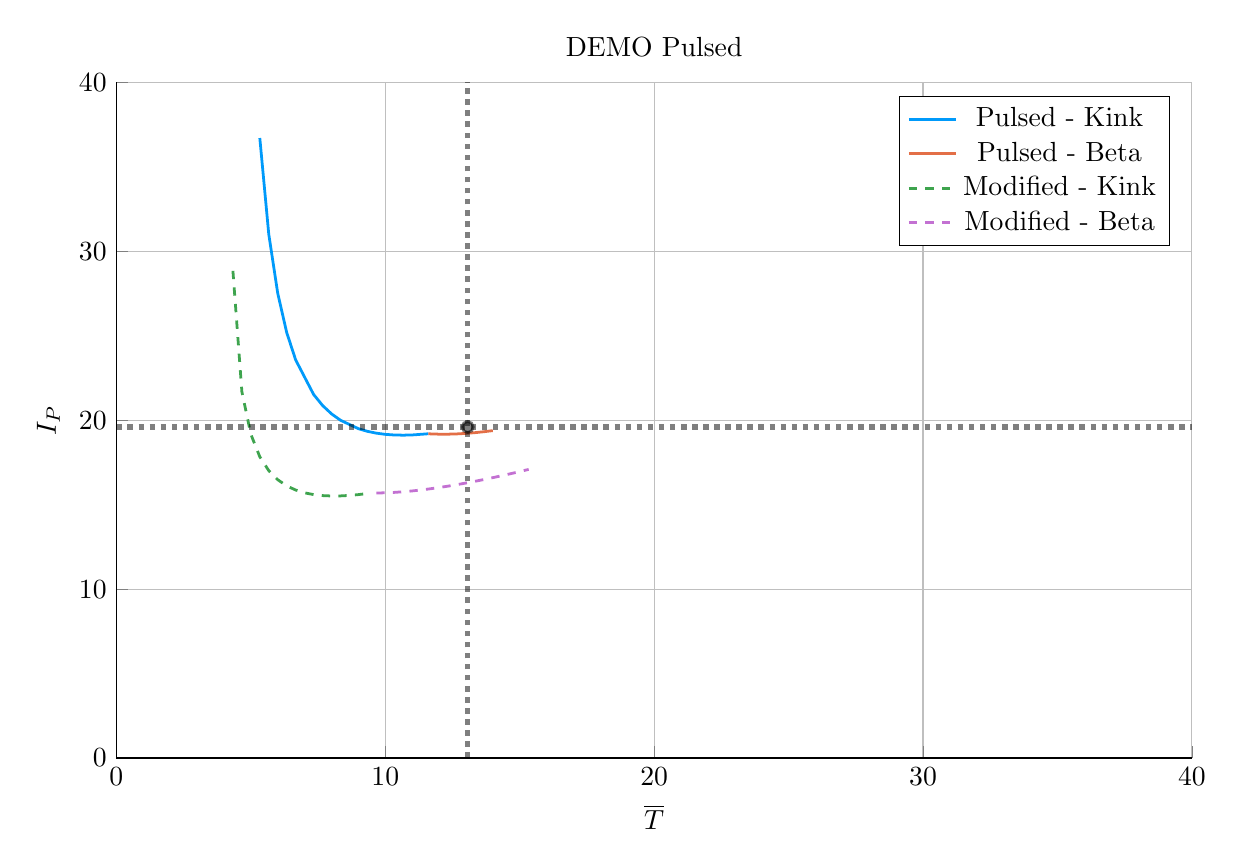
\begin{tikzpicture}[]
\begin{axis}[height = {101.6mm}, ylabel = {${I}_{P}$}, title = {DEMO Pulsed}, xmin = {0.0}, xmax = {40.0}, ymax = {40.0}, xlabel = {$\overline {T}$}, {unbounded coords=jump, scaled x ticks = false, xticklabel style={rotate = 0}, xmajorgrids = true, xtick = {0.0,10.0,20.0,30.0,40.0}, xticklabels = {0,10,20,30,40}, xtick align = inside, axis lines* = left, scaled y ticks = false, yticklabel style={rotate = 0}, ymajorgrids = true, ytick = {0.0,10.0,20.0,30.0,40.0}, yticklabels = {0,10,20,30,40}, ytick align = inside, axis lines* = left,     xshift = 0.0mm,
    yshift = 0.0mm,
    axis background/.style={fill={rgb,1:red,1.00000000;green,1.00000000;blue,1.00000000}}
, colorbar style={title=}}, ymin = {0.0}, width = {152.4mm}]\addplot+ [color = {rgb,1:red,0.00000000;green,0.60560316;blue,0.97868012},
draw opacity=1.0,
line width=1,
solid,mark = none,
mark size = 2.0,
mark options = {
    color = {rgb,1:red,0.00000000;green,0.00000000;blue,0.00000000}, draw opacity = 1.0,
    fill = {rgb,1:red,0.00000000;green,0.60560316;blue,0.97868012}, fill opacity = 1.0,
    line width = 1,
    rotate = 0,
    solid
}]coordinates {
(5.333333333333333, 36.71051032912112)
(5.666666666666667, 31.014995367356207)
(6.0, 27.51734786322149)
(6.333333333333333, 25.19534286389616)
(6.666666666666667, 23.57285610926683)
(7.333333333333333, 21.52905816503197)
(7.666666666666667, 20.874444053021588)
(8.0, 20.377542510464334)
(8.333333333333334, 19.99951688957442)
(9.0, 19.499202175706746)
(9.333333333333334, 19.343044014643887)
(9.666666666666666, 19.233955791269285)
(10.0, 19.16365729524907)
(10.333333333333334, 19.125701869840853)
(10.666666666666666, 19.11499858904485)
(11.0, 19.127475979338943)
(11.600962879632572, 19.198383823705257)
};
\addlegendentry{Pulsed - Kink}
\addplot+ [color = {rgb,1:red,0.88887350;green,0.43564919;blue,0.27812294},
draw opacity=1.0,
line width=1,
solid,mark = none,
mark size = 2.0,
mark options = {
    color = {rgb,1:red,0.00000000;green,0.00000000;blue,0.00000000}, draw opacity = 1.0,
    fill = {rgb,1:red,0.88887350;green,0.43564919;blue,0.27812294}, fill opacity = 1.0,
    line width = 1,
    rotate = 0,
    solid
}]coordinates {
(11.600962879632572, 19.198383823705257)
(11.666666666666666, 19.192414153878335)
(12.0, 19.174087186739918)
(12.333333333333334, 19.17397121853779)
(12.666666666666666, 19.189978018951553)
(13.0, 19.220357277326283)
(13.333333333333334, 19.263633100211838)
(13.666666666666666, 19.31855421750887)
(14.0, 19.384054548489104)
};
\addlegendentry{Pulsed - Beta}
\addplot+ [color = {rgb,1:red,0.24222430;green,0.64327509;blue,0.30444865},
draw opacity=1.0,
line width=1,
dashed,mark = none,
mark size = 2.0,
mark options = {
    color = {rgb,1:red,0.00000000;green,0.00000000;blue,0.00000000}, draw opacity = 1.0,
    fill = {rgb,1:red,0.24222430;green,0.64327509;blue,0.30444865}, fill opacity = 1.0,
    line width = 1,
    rotate = 0,
    solid
}]coordinates {
(4.333333333333333, 28.845639077165217)
(4.666666666666667, 21.687713986294685)
(5.0, 19.170340224057398)
(5.333333333333333, 17.83397336320386)
(5.666666666666667, 17.01478565989059)
(6.0, 16.477486603636205)
(6.333333333333333, 16.113958654578386)
(6.666666666666667, 15.866460603971907)
(7.0, 15.700928946757587)
(7.333333333333333, 15.59578560596909)
(7.666666666666667, 15.536607983152381)
(8.0, 15.513342675582972)
(8.333333333333334, 15.518740955012225)
(8.666666666666666, 15.547428978968492)
(9.0, 15.595329068459918)
(9.333333333333334, 15.659285368310089)
};
\addlegendentry{Modified - Kink}
\addplot+ [color = {rgb,1:red,0.76444018;green,0.44411178;blue,0.82429754},
draw opacity=1.0,
line width=1,
dashed,mark = none,
mark size = 2.0,
mark options = {
    color = {rgb,1:red,0.00000000;green,0.00000000;blue,0.00000000}, draw opacity = 1.0,
    fill = {rgb,1:red,0.76444018;green,0.44411178;blue,0.82429754}, fill opacity = 1.0,
    line width = 1,
    rotate = 0,
    solid
}]coordinates {
(9.666666666666666, 15.691192911261952)
(10.0, 15.70165788278533)
(10.333333333333334, 15.726578234093749)
(10.666666666666666, 15.764127054896537)
(11.0, 15.812802650736373)
(11.333333333333334, 15.871360766004056)
(11.666666666666666, 15.938763317563621)
(12.0, 16.014139065408)
(12.333333333333334, 16.09675304572932)
(12.666666666666666, 16.185982524147033)
(13.0, 16.281297862810217)
(13.333333333333334, 16.382247130746602)
(13.666666666666666, 16.488443597982137)
(14.0, 16.5995554722192)
(14.333333333333334, 16.715297396529092)
(14.666666666666666, 16.83542334285969)
(15.0, 16.959720624053933)
(15.333333333333334, 17.088004807739882)
};
\addlegendentry{Modified - Beta}
\addplot+ [color = {rgb,1:red,0.00000000;green,0.00000000;blue,0.00000000},
draw opacity=0.5,
line width=2,
dotted,mark = none,
mark size = 2.0,
mark options = {
    color = {rgb,1:red,0.00000000;green,0.00000000;blue,0.00000000}, draw opacity = 0.5,
    fill = {rgb,1:red,0.00000000;green,0.00000000;blue,0.00000000}, fill opacity = 0.5,
    line width = 1,
    rotate = 0,
    solid
},forget plot]coordinates {
(0.0, 19.6)
(40.0, 19.6)
};
\addplot+ [color = {rgb,1:red,0.00000000;green,0.00000000;blue,0.00000000},
draw opacity=0.5,
line width=2,
dotted,mark = none,
mark size = 2.0,
mark options = {
    color = {rgb,1:red,0.00000000;green,0.00000000;blue,0.00000000}, draw opacity = 0.5,
    fill = {rgb,1:red,0.00000000;green,0.00000000;blue,0.00000000}, fill opacity = 0.5,
    line width = 1,
    rotate = 0,
    solid
},forget plot]coordinates {
(13.065, 0.0)
(13.065, 40.0)
};
\addplot+[draw=none, color = {rgb,1:red,0.00000000;green,0.00000000;blue,0.00000000},
draw opacity=0.5,
line width=0,
solid,mark = *,
mark size = 2.0,
mark options = {
    color = {rgb,1:red,0.00000000;green,0.00000000;blue,0.00000000}, draw opacity = 0.5,
    fill = {rgb,1:red,0.00000000;green,0.00000000;blue,0.00000000}, fill opacity = 0.5,
    line width = 1,
    rotate = 0,
    solid
},forget plot] coordinates {
(13.065, 19.6)
};
\end{axis}

\end{tikzpicture}

    \end{adjustbox}
        \caption{$I_P$ vs $\overline T$}
    \end{subfigure}
    \hfill \hfill ~\\ ~\\ ~\\
    \caption{Demo Pulsed Model Comparison} ~\\
\end{figure*}

\begin{table}[h!]
\centering  
\caption{Demo Pulsed Variables}
\hfill
\begin{subtable}[t]{0.4\textwidth}
\centering  
\caption{Input Variables} ~\\
\begin{tabular}{ c|c } 

Input            & Value           \\
\hline
$H$              & 1.1             \\
$Q$              & 39.86           \\
$N_{G}$          & 1.2             \\
$\epsilon$       & 0.3226          \\
$\kappa_{95}$    & 1.59            \\
$\delta_{95}$    & 0.333           \\
$\nu_{n}$        & 0.27            \\
$\nu_{T}$        & 1.094           \\
$l_{i}$          & 1.155           \\
$A$              & 2.735           \\
$Z_{eff}$        & 2.584           \\
$f_{D}$          & 0.7753          \\
$\tau_{FT}$      & 7273          \\
$B_{CS}$         & 12.77           \\

\end{tabular}
\end{subtable}
\hfill
\begin{subtable}[t]{0.5\textwidth}
\centering  
\caption{Output Variables} ~\\
\begin{tabular}{ c|c|c } 

Output           & Original         & Fussy.jl        \\
\hline
$R_{0}$          & 9.07            & 8.10             \\
$B_{0}$          & 5.67            & 5.48            \\
$I_{P}$          & 19.6             & 19.3           \\
$\overline n$    & 0.7983           & 0.9795          \\
$\overline T$    & 13.06            & 13.28           \\
$\beta_{N}$       & 0.0259           & -          \\
$q_{95}$         & 3.247            & 2.853           \\
$P_{W}$          & 1.05             & 1.47           \\
$f_{BS}$         & 0.348            & 0.164          \\
$f_{CD}$         & 0.096            & 0.106          \\
$f_{IN}$         & 0.557            & 0.730          \\
$\volume$         & 2502           & 1751          \\
$P_{F}$          & 2037           & 2376          \\
$\eta_{CD}$      & 0.2721           & -     

\end{tabular}
\end{subtable}
\hfill
\hfill
\end{table}

\section{Developing Prototype Reactors}

Now that the model used in Fussy.jl has been tested against other fusion systems codes in the field, we will develop our own prototype reactors. Because this paper is about making a levelized comparison of pulsed and steady-state tokamaks, we will develop middle-of-the-road reactors that only differ by operating mode. 

The steady-state prototype, Charybdis, is the obvious choice to start with -- as the model was tested against four of these typed reactors. It was also pointed out that the model did remarkably well when recreating ARC. As the authors share many of the ARC team's philosophies, Charybdis uses fixed parameters very similar to them.

Next, although led to believe Charybdis' pulsed twin reactor -- Proteus -- would be created by a simple flip of the switch, it was a slight oversimplification. The first difference is that the pulsed twin, Proteus, is assumed to be purely pulsed: $\eta_{CD} = 0$. Further, the bootstrap current is much less important than it was for steady-state tokamaks. This corresponds to a current profile peaked at the origin -- i.e. a parabola. Numerically, this is done by raising $l_i$ from around 5.5 to 6.

The final difference creates the largest change in the twin reactors: the choice of miracle. As hinted several times before, the H factor is a common way designers artificially boost the confinement of their machines. This H value will thus be the miracle for Charybdis, the steady-state prototype. Next, as the main conclusion of this paper is to state the advantages of high magnetic field, a free way to boost a central solenoid using HTS coils will be employed.

Opposite the order of how they were designed, the goal now is to lock down a value of $B_{CS}$ for Proteus and then use it to set the H factor for Charybdis. This selection algorithm is depicted in \cref{fig:selection}. For Proteus, the point locked down was $B_{CS} = 20 \ \textnormal{T}$, which occurred at a fusion power ($P_F$) of around 1250 MW. As shown in the cost curve, this was at a point where the ratio between the minimum capital cost and the minimum cost-per-watt saturated. This choice of a 1250 MW reactor then led to Charybdis having an H factor of 1.7.

\begin{figure}[h!]
\centering
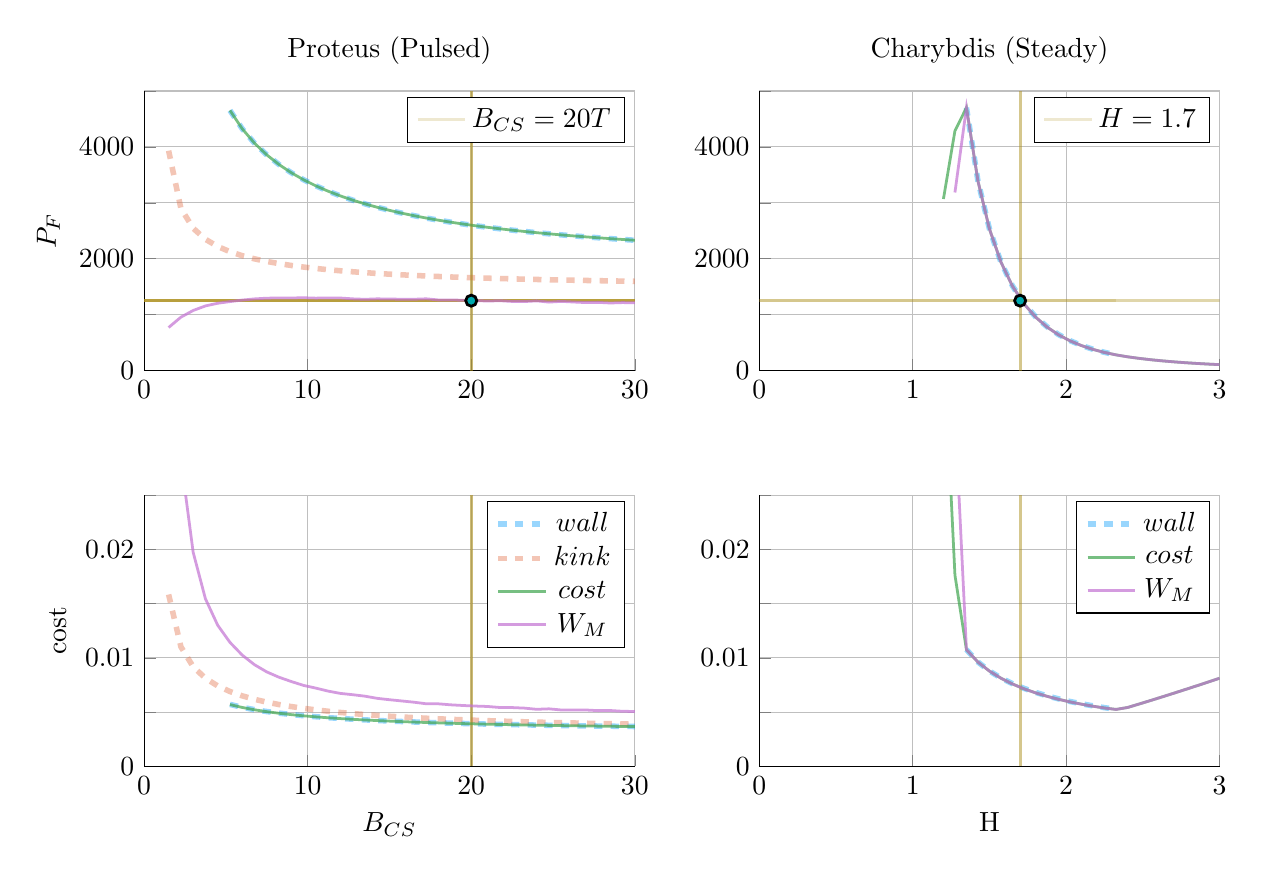
\begin{tikzpicture}[]
\begin{axis}[height = {51.32916666666667mm}, ylabel = {$P_F$}, title = {Proteus (Pulsed)}, xmin = {0}, xmax = {30.0}, ymax = {5000.0}, xlabel = {}, {unbounded coords=jump, scaled x ticks = false, xticklabel style={rotate = 0}, xmajorgrids = true, xtick = {0.0,10.0,20.0,30.0}, xticklabels = {0,10,20,30}, xtick align = inside, axis lines* = left, scaled y ticks = false, yticklabel style={rotate = 0}, ymajorgrids = true, ytick = {0,1000,2000,3000,4000,5000}, yticklabels = {0,,2000,,4000,}, ytick align = inside, axis lines* = left,     xshift = 0.0mm,
    yshift = 50.27mm,
    axis background/.style={fill={rgb,1:red,1.00000000;green,1.00000000;blue,1.00000000}}
}, ymin = {2.220446049250313e-16}, width = {78.14027777777778mm}]\addplot+ [color = {rgb,1:red,0.67554396;green,0.55566233;blue,0.09423434},
draw opacity=0.2,
line width=1,
solid,mark = none,
mark size = 2.0,
mark options = {
    color = {rgb,1:red,0.00000000;green,0.00000000;blue,0.00000000}, draw opacity = 1.0,
    fill = {rgb,1:red,0.67554396;green,0.55566233;blue,0.09423434}, fill opacity = 1.0,
    line width = 1,
    rotate = 0,
    solid
}]coordinates {
(20.0, 2.220446049250313e-16)
(20.0, 5000.0)
};
\addlegendentry{$B_{CS} = 20 T$}
\addplot+ [color = {rgb,1:red,0.67554396;green,0.55566233;blue,0.09423434},
draw opacity=0.2,
line width=1,
solid,mark = none,
mark size = 2.0,
mark options = {
    color = {rgb,1:red,0.00000000;green,0.00000000;blue,0.00000000}, draw opacity = 1.0,
    fill = {rgb,1:red,0.67554396;green,0.55566233;blue,0.09423434}, fill opacity = 1.0,
    line width = 1,
    rotate = 0,
    solid
},forget plot]coordinates {
(0.0, 1250.0)
(30.0, 1250.0)
};
\addplot+[draw=none, color = {rgb,1:red,0.00000048;green,0.66575898;blue,0.68099695},
draw opacity=1.0,
line width=0,
solid,mark = *,
mark size = 2.0,
mark options = {
    color = {rgb,1:red,0.00000000;green,0.00000000;blue,0.00000000}, draw opacity = 1.0,
    fill = {rgb,1:red,0.00000048;green,0.66575898;blue,0.68099695}, fill opacity = 1.0,
    line width = 1,
    rotate = 0,
    solid
},forget plot] coordinates {
(20, 1250)
};
\addplot+ [color = {rgb,1:red,0.67554396;green,0.55566233;blue,0.09423434},
draw opacity=0.2,
line width=1,
solid,mark = none,
mark size = 2.0,
mark options = {
    color = {rgb,1:red,0.00000000;green,0.00000000;blue,0.00000000}, draw opacity = 1.0,
    fill = {rgb,1:red,0.67554396;green,0.55566233;blue,0.09423434}, fill opacity = 1.0,
    line width = 1,
    rotate = 0,
    solid
},forget plot]coordinates {
(0.0, 1250.0)
(30.0, 1250.0)
};
\addplot+ [color = {rgb,1:red,0.00000000;green,0.60560316;blue,0.97868012},
draw opacity=0.4,
line width=2,
dashed,mark = none,
mark size = 2.0,
mark options = {
    color = {rgb,1:red,0.00000000;green,0.00000000;blue,0.00000000}, draw opacity = 1.0,
    fill = {rgb,1:red,0.00000000;green,0.60560316;blue,0.97868012}, fill opacity = 1.0,
    line width = 1,
    rotate = 0,
    solid
},forget plot]coordinates {
(5.25, 4651.734735476011)
(6.0, 4323.6250098364)
(6.75, 4065.99692078527)
(7.5, 3857.273578687972)
(8.25, 3684.1342593418663)
(9.0, 3537.844669896544)
(9.75, 3412.404653539425)
(10.5, 3303.536032694244)
(11.25, 3208.094051273514)
(12.0, 3123.707522754923)
(12.75, 3048.5495054628623)
(13.5, 2981.185980181023)
(14.25, 2920.472987010462)
(15.0, 2865.484885250518)
(15.75, 2815.463186166668)
(16.5, 2769.7793320244814)
(17.25, 2727.9071420752607)
(18.0, 2689.4020933235493)
(18.75, 2653.885520176901)
(19.5, 2621.0324111911764)
(20.25, 2590.561874678777)
(21.0, 2562.2296107375955)
(21.75, 2535.8219099446264)
(22.5, 2511.150826555893)
(23.25, 2488.050264495335)
(24.0, 2466.372779394113)
(24.75, 2445.986947213969)
(25.5, 2426.775184780072)
(26.25, 2408.6319334297787)
(27.0, 2391.4621364565396)
(27.75, 2375.1799557182867)
(28.5, 2359.707684182671)
(29.25, 2344.974819785335)
(30.0, 2330.917272823136)
};
\addplot+ [color = {rgb,1:red,0.67554396;green,0.55566233;blue,0.09423434},
draw opacity=0.2,
line width=1,
solid,mark = none,
mark size = 2.0,
mark options = {
    color = {rgb,1:red,0.00000000;green,0.00000000;blue,0.00000000}, draw opacity = 1.0,
    fill = {rgb,1:red,0.67554396;green,0.55566233;blue,0.09423434}, fill opacity = 1.0,
    line width = 1,
    rotate = 0,
    solid
},forget plot]coordinates {
(20.0, 2.220446049250313e-16)
(20.0, 5000.0)
};
\addplot+ [color = {rgb,1:red,0.67554396;green,0.55566233;blue,0.09423434},
draw opacity=0.2,
line width=1,
solid,mark = none,
mark size = 2.0,
mark options = {
    color = {rgb,1:red,0.00000000;green,0.00000000;blue,0.00000000}, draw opacity = 1.0,
    fill = {rgb,1:red,0.67554396;green,0.55566233;blue,0.09423434}, fill opacity = 1.0,
    line width = 1,
    rotate = 0,
    solid
},forget plot]coordinates {
(0.0, 1250.0)
(30.0, 1250.0)
};
\addplot+ [color = {rgb,1:red,0.67554396;green,0.55566233;blue,0.09423434},
draw opacity=0.2,
line width=1,
solid,mark = none,
mark size = 2.0,
mark options = {
    color = {rgb,1:red,0.00000000;green,0.00000000;blue,0.00000000}, draw opacity = 1.0,
    fill = {rgb,1:red,0.67554396;green,0.55566233;blue,0.09423434}, fill opacity = 1.0,
    line width = 1,
    rotate = 0,
    solid
},forget plot]coordinates {
(0.0, 1250.0)
(30.0, 1250.0)
};
\addplot+ [color = {rgb,1:red,0.88887350;green,0.43564919;blue,0.27812294},
draw opacity=0.4,
line width=2,
dashed,mark = none,
mark size = 2.0,
mark options = {
    color = {rgb,1:red,0.00000000;green,0.00000000;blue,0.00000000}, draw opacity = 1.0,
    fill = {rgb,1:red,0.88887350;green,0.43564919;blue,0.27812294}, fill opacity = 1.0,
    line width = 1,
    rotate = 0,
    solid
},forget plot]coordinates {
(1.5, 3931.6170696070676)
(2.25, 2900.7235747979908)
(3.0, 2544.8446560898715)
(3.75, 2348.228116500571)
(4.5, 2219.0134794713767)
(5.25, 2125.815532966674)
(6.0, 2054.566085735622)
(6.75, 1997.8824990557177)
(7.5, 1951.4633680592258)
(8.25, 1912.6074536455505)
(9.0, 1879.5196356674505)
(9.75, 1850.953068441656)
(10.5, 1826.0101459658863)
(11.25, 1804.02551415983)
(12.0, 1784.493638745381)
(12.75, 1767.0222758941622)
(13.5, 1751.3015387280175)
(14.25, 1737.0827328069474)
(15.0, 1724.1634044428295)
(15.75, 1712.376890482151)
(16.5, 1701.5841921715175)
(17.25, 1691.6685698179294)
(18.0, 1682.530881991843)
(18.75, 1674.0861755860074)
(19.5, 1666.2615100001372)
(20.25, 1658.9932835127363)
(21.0, 1652.2262595201232)
(21.75, 1645.91179207308)
(22.5, 1640.0070406407558)
(23.25, 1634.4738680952948)
(24.0, 1629.2785569006053)
(24.75, 1624.3908184475338)
(25.5, 1619.7835209277835)
(26.25, 1615.432247074283)
(27.0, 1611.314956936522)
(27.75, 1607.4117026157203)
(28.5, 1603.7043856927105)
(29.25, 1600.1765499289672)
(30.0, 1596.813203261599)
};
\addplot+ [color = {rgb,1:red,0.67554396;green,0.55566233;blue,0.09423434},
draw opacity=0.2,
line width=1,
solid,mark = none,
mark size = 2.0,
mark options = {
    color = {rgb,1:red,0.00000000;green,0.00000000;blue,0.00000000}, draw opacity = 1.0,
    fill = {rgb,1:red,0.67554396;green,0.55566233;blue,0.09423434}, fill opacity = 1.0,
    line width = 1,
    rotate = 0,
    solid
},forget plot]coordinates {
(20.0, 2.220446049250313e-16)
(20.0, 5000.0)
};
\addplot+ [color = {rgb,1:red,0.67554396;green,0.55566233;blue,0.09423434},
draw opacity=0.2,
line width=1,
solid,mark = none,
mark size = 2.0,
mark options = {
    color = {rgb,1:red,0.00000000;green,0.00000000;blue,0.00000000}, draw opacity = 1.0,
    fill = {rgb,1:red,0.67554396;green,0.55566233;blue,0.09423434}, fill opacity = 1.0,
    line width = 1,
    rotate = 0,
    solid
},forget plot]coordinates {
(0.0, 1250.0)
(30.0, 1250.0)
};
\addplot+ [color = {rgb,1:red,0.67554396;green,0.55566233;blue,0.09423434},
draw opacity=0.2,
line width=1,
solid,mark = none,
mark size = 2.0,
mark options = {
    color = {rgb,1:red,0.00000000;green,0.00000000;blue,0.00000000}, draw opacity = 1.0,
    fill = {rgb,1:red,0.67554396;green,0.55566233;blue,0.09423434}, fill opacity = 1.0,
    line width = 1,
    rotate = 0,
    solid
},forget plot]coordinates {
(0.0, 1250.0)
(30.0, 1250.0)
};
\addplot+ [color = {rgb,1:red,0.24222430;green,0.64327509;blue,0.30444865},
draw opacity=0.7,
line width=1,
solid,mark = none,
mark size = 2.0,
mark options = {
    color = {rgb,1:red,0.00000000;green,0.00000000;blue,0.00000000}, draw opacity = 1.0,
    fill = {rgb,1:red,0.24222430;green,0.64327509;blue,0.30444865}, fill opacity = 1.0,
    line width = 1,
    rotate = 0,
    solid
},forget plot]coordinates {
(5.25, 4651.856974626446)
(6.0, 4323.626574700689)
(6.75, 4065.9133365013354)
(7.5, 3857.1264771824617)
(8.25, 3683.9377449687768)
(9.0, 3537.608432111376)
(9.75, 3412.1356303067523)
(10.5, 3303.239361854739)
(11.25, 3207.7736468791713)
(12.0, 3123.3664382128795)
(12.75, 3048.1901722862794)
(13.5, 2980.810371417949)
(14.25, 2920.082728006143)
(15.0, 2865.081335141082)
(15.75, 2815.0474968726217)
(16.5, 2769.352491750233)
(17.25, 2727.4700069605415)
(18.0, 2688.955412764386)
(18.75, 2653.4299583736)
(19.5, 2620.5685580410595)
(20.25, 2590.0902617025704)
(21.0, 2561.7507209540713)
(21.75, 2535.3361812985195)
(22.5, 2510.65866319561)
(23.25, 2487.5520396570964)
(24.0, 2465.868837737164)
(24.75, 2445.477613655657)
(25.5, 2426.2607621440256)
(26.25, 2408.1127073411044)
(27.0, 2390.9383771738235)
(27.75, 2374.651919394813)
(28.5, 2359.1756148307045)
(29.25, 2344.438950143004)
(30.0, 2330.377825995788)
};
\addplot+ [color = {rgb,1:red,0.67554396;green,0.55566233;blue,0.09423434},
draw opacity=0.2,
line width=1,
solid,mark = none,
mark size = 2.0,
mark options = {
    color = {rgb,1:red,0.00000000;green,0.00000000;blue,0.00000000}, draw opacity = 1.0,
    fill = {rgb,1:red,0.67554396;green,0.55566233;blue,0.09423434}, fill opacity = 1.0,
    line width = 1,
    rotate = 0,
    solid
},forget plot]coordinates {
(20.0, 2.220446049250313e-16)
(20.0, 5000.0)
};
\addplot+ [color = {rgb,1:red,0.67554396;green,0.55566233;blue,0.09423434},
draw opacity=0.2,
line width=1,
solid,mark = none,
mark size = 2.0,
mark options = {
    color = {rgb,1:red,0.00000000;green,0.00000000;blue,0.00000000}, draw opacity = 1.0,
    fill = {rgb,1:red,0.67554396;green,0.55566233;blue,0.09423434}, fill opacity = 1.0,
    line width = 1,
    rotate = 0,
    solid
},forget plot]coordinates {
(0.0, 1250.0)
(30.0, 1250.0)
};
\addplot+ [color = {rgb,1:red,0.67554396;green,0.55566233;blue,0.09423434},
draw opacity=0.2,
line width=1,
solid,mark = none,
mark size = 2.0,
mark options = {
    color = {rgb,1:red,0.00000000;green,0.00000000;blue,0.00000000}, draw opacity = 1.0,
    fill = {rgb,1:red,0.67554396;green,0.55566233;blue,0.09423434}, fill opacity = 1.0,
    line width = 1,
    rotate = 0,
    solid
},forget plot]coordinates {
(0.0, 1250.0)
(30.0, 1250.0)
};
\addplot+ [color = {rgb,1:red,0.76444018;green,0.44411178;blue,0.82429754},
draw opacity=0.7,
line width=1,
solid,mark = none,
mark size = 2.0,
mark options = {
    color = {rgb,1:red,0.00000000;green,0.00000000;blue,0.00000000}, draw opacity = 1.0,
    fill = {rgb,1:red,0.76444018;green,0.44411178;blue,0.82429754}, fill opacity = 1.0,
    line width = 1,
    rotate = 0,
    solid
},forget plot]coordinates {
(1.5, 770.4535163440595)
(2.25, 954.8730192598816)
(3.0, 1074.7019495723541)
(3.75, 1156.024788273215)
(4.5, 1204.0200711633677)
(5.25, 1233.7948079824048)
(6.0, 1260.6547091987875)
(6.75, 1281.8429530808678)
(7.5, 1294.6082412516207)
(8.25, 1298.1292122440111)
(9.0, 1298.1210010392879)
(9.75, 1302.223238135332)
(10.5, 1295.054060000207)
(11.25, 1299.5652880713872)
(12.0, 1297.6289491073692)
(12.75, 1282.6829774082355)
(13.5, 1274.473146838615)
(14.25, 1282.8743293523935)
(15.0, 1279.4366420169024)
(15.75, 1276.1045609204925)
(16.5, 1275.52105613002)
(17.25, 1283.4690177878747)
(18.0, 1262.712514215648)
(18.75, 1262.7843385038082)
(19.5, 1257.6056644505838)
(20.25, 1251.4051011388665)
(21.0, 1243.4899440635038)
(21.75, 1249.4484707880504)
(22.5, 1236.3207332951713)
(23.25, 1234.0894652277675)
(24.0, 1246.6870760568188)
(24.75, 1224.0642650291306)
(25.5, 1237.4485384154398)
(26.25, 1226.0446362827531)
(27.0, 1215.9720878560222)
(27.75, 1219.8261291156418)
(28.5, 1208.2813208095588)
(29.25, 1215.812124675399)
(30.0, 1211.4870892754757)
};
\end{axis}
\begin{axis}[height = {51.32916666666667mm}, ylabel = {}, title = {Charybdis (Steady)}, xmin = {0}, xmax = {3.0}, ymax = {5000.0}, xlabel = {}, {unbounded coords=jump, scaled x ticks = false, xticklabel style={rotate = 0}, xmajorgrids = true, xtick = {0.0,1.0,2.0,3.0}, xticklabels = {0,1,2,3}, xtick align = inside, axis lines* = left, scaled y ticks = false, yticklabel style={rotate = 0}, ymajorgrids = true, ytick = {0,1000,2000,3000,4000,5000}, yticklabels = {0,,2000,,4000,}, ytick align = inside, axis lines* = left,     xshift = 78.14027777777778mm,
    yshift = 50.27mm,
    axis background/.style={fill={rgb,1:red,1.00000000;green,1.00000000;blue,1.00000000}}
}, ymin = {2.220446049250313e-16}, width = {74.25972222222222mm}]\addplot+ [color = {rgb,1:red,0.67554396;green,0.55566233;blue,0.09423434},
draw opacity=0.2,
line width=1,
solid,mark = none,
mark size = 2.0,
mark options = {
    color = {rgb,1:red,0.00000000;green,0.00000000;blue,0.00000000}, draw opacity = 1.0,
    fill = {rgb,1:red,0.67554396;green,0.55566233;blue,0.09423434}, fill opacity = 1.0,
    line width = 1,
    rotate = 0,
    solid
}]coordinates {
(1.7, 2.220446049250313e-16)
(1.7, 5000.0)
};
\addlegendentry{$H = 1.7$}
\addplot+ [color = {rgb,1:red,0.67554396;green,0.55566233;blue,0.09423434},
draw opacity=0.2,
line width=1,
solid,mark = none,
mark size = 2.0,
mark options = {
    color = {rgb,1:red,0.00000000;green,0.00000000;blue,0.00000000}, draw opacity = 1.0,
    fill = {rgb,1:red,0.67554396;green,0.55566233;blue,0.09423434}, fill opacity = 1.0,
    line width = 1,
    rotate = 0,
    solid
},forget plot]coordinates {
(0.0, 1250.0)
(2.325, 1250.0)
};
\addplot+[draw=none, color = {rgb,1:red,0.00000048;green,0.66575898;blue,0.68099695},
draw opacity=1.0,
line width=0,
solid,mark = *,
mark size = 2.0,
mark options = {
    color = {rgb,1:red,0.00000000;green,0.00000000;blue,0.00000000}, draw opacity = 1.0,
    fill = {rgb,1:red,0.00000048;green,0.66575898;blue,0.68099695}, fill opacity = 1.0,
    line width = 1,
    rotate = 0,
    solid
},forget plot] coordinates {
(1.7, 1250.0)
};
\addplot+ [color = {rgb,1:red,0.00000000;green,0.60560316;blue,0.97868012},
draw opacity=0.4,
line width=2,
dashed,mark = none,
mark size = 2.0,
mark options = {
    color = {rgb,1:red,0.00000000;green,0.00000000;blue,0.00000000}, draw opacity = 1.0,
    fill = {rgb,1:red,0.00000000;green,0.60560316;blue,0.97868012}, fill opacity = 1.0,
    line width = 1,
    rotate = 0,
    solid
},forget plot]coordinates {
(1.35, 4702.419771261358)
(1.425, 3389.739729501066)
(1.5, 2531.7367375233785)
(1.575, 1938.5570892600988)
(1.65, 1513.711721274854)
(1.725, 1200.1687454499686)
(1.8, 964.3328758303221)
(1.875, 784.1982422273053)
(1.95, 644.8519631594907)
(2.025, 535.8348429353653)
(2.1, 449.6995270356)
(2.175, 381.0209603225493)
(2.25, 325.79222945707494)
(2.325, 281.0170460687302)
};
\addplot+ [color = {rgb,1:red,0.67554396;green,0.55566233;blue,0.09423434},
draw opacity=0.2,
line width=1,
solid,mark = none,
mark size = 2.0,
mark options = {
    color = {rgb,1:red,0.00000000;green,0.00000000;blue,0.00000000}, draw opacity = 1.0,
    fill = {rgb,1:red,0.67554396;green,0.55566233;blue,0.09423434}, fill opacity = 1.0,
    line width = 1,
    rotate = 0,
    solid
},forget plot]coordinates {
(1.7, 2.220446049250313e-16)
(1.7, 5000.0)
};
\addplot+ [color = {rgb,1:red,0.67554396;green,0.55566233;blue,0.09423434},
draw opacity=0.2,
line width=1,
solid,mark = none,
mark size = 2.0,
mark options = {
    color = {rgb,1:red,0.00000000;green,0.00000000;blue,0.00000000}, draw opacity = 1.0,
    fill = {rgb,1:red,0.67554396;green,0.55566233;blue,0.09423434}, fill opacity = 1.0,
    line width = 1,
    rotate = 0,
    solid
},forget plot]coordinates {
(0.0, 1250.0)
(3.0, 1250.0)
};
\addplot+ [color = {rgb,1:red,0.24222430;green,0.64327509;blue,0.30444865},
draw opacity=0.7,
line width=1,
solid,mark = none,
mark size = 2.0,
mark options = {
    color = {rgb,1:red,0.00000000;green,0.00000000;blue,0.00000000}, draw opacity = 1.0,
    fill = {rgb,1:red,0.24222430;green,0.64327509;blue,0.30444865}, fill opacity = 1.0,
    line width = 1,
    rotate = 0,
    solid
},forget plot]coordinates {
(1.2, 3068.343606355172)
(1.275, 4286.260736815682)
(1.35, 4701.710701951617)
(1.425, 3388.877819042802)
(1.5, 2531.10959033651)
(1.575, 1938.9724494012169)
(1.65, 1509.401812434612)
(1.725, 1194.4826335617477)
(1.8, 958.6889855821258)
(1.875, 779.1702454071224)
(1.95, 640.597451863543)
(2.025, 532.3571298076668)
(2.1, 446.9177644738313)
(2.175, 378.82904019299)
(2.25, 324.08335892453823)
(2.325, 281.0958675842298)
(2.4, 246.5983680765812)
(2.475, 218.57873818292612)
(2.55, 194.68877419879524)
(2.625, 174.21242277866037)
(2.7, 156.57438414009331)
(2.775, 141.30840500712233)
(2.85, 128.03547590420067)
(2.925, 116.44528649040114)
(3.0, 106.28251642550786)
};
\addplot+ [color = {rgb,1:red,0.67554396;green,0.55566233;blue,0.09423434},
draw opacity=0.2,
line width=1,
solid,mark = none,
mark size = 2.0,
mark options = {
    color = {rgb,1:red,0.00000000;green,0.00000000;blue,0.00000000}, draw opacity = 1.0,
    fill = {rgb,1:red,0.67554396;green,0.55566233;blue,0.09423434}, fill opacity = 1.0,
    line width = 1,
    rotate = 0,
    solid
},forget plot]coordinates {
(1.7, 2.220446049250313e-16)
(1.7, 5000.0)
};
\addplot+ [color = {rgb,1:red,0.67554396;green,0.55566233;blue,0.09423434},
draw opacity=0.2,
line width=1,
solid,mark = none,
mark size = 2.0,
mark options = {
    color = {rgb,1:red,0.00000000;green,0.00000000;blue,0.00000000}, draw opacity = 1.0,
    fill = {rgb,1:red,0.67554396;green,0.55566233;blue,0.09423434}, fill opacity = 1.0,
    line width = 1,
    rotate = 0,
    solid
},forget plot]coordinates {
(0.0, 1250.0)
(3.0, 1250.0)
};
\addplot+ [color = {rgb,1:red,0.76444018;green,0.44411178;blue,0.82429754},
draw opacity=0.7,
line width=1,
solid,mark = none,
mark size = 2.0,
mark options = {
    color = {rgb,1:red,0.00000000;green,0.00000000;blue,0.00000000}, draw opacity = 1.0,
    fill = {rgb,1:red,0.76444018;green,0.44411178;blue,0.82429754}, fill opacity = 1.0,
    line width = 1,
    rotate = 0,
    solid
},forget plot]coordinates {
(1.275, 3184.7544513979055)
(1.35, 4702.336497990941)
(1.425, 3388.9574757185483)
(1.5, 2531.1205717652433)
(1.575, 1938.799888683301)
(1.65, 1508.8938538316263)
(1.725, 1193.8896388912244)
(1.8, 958.1150115203263)
(1.875, 778.6581601462384)
(1.95, 640.1615648471053)
(2.025, 531.9977422035347)
(2.1, 446.62839995026565)
(2.175, 378.60033344126833)
(2.25, 323.90523713971857)
(2.325, 280.72617729356347)
(2.4, 246.59420337797187)
(2.475, 218.57531693530026)
(2.55, 194.6859804122245)
(2.625, 174.2102899084507)
(2.7, 156.57254493780485)
(2.775, 141.30691976562986)
(2.85, 128.0342791712537)
(2.925, 116.44432378465737)
(3.0, 106.2817429069081)
};
\end{axis}
\begin{axis}[height = {50.27083333333333mm}, ylabel = {cost}, xmin = {0}, xmax = {30.0}, ymax = {0.025}, xlabel = {$B_{CS}$}, {unbounded coords=jump, scaled x ticks = false, xticklabel style={rotate = 0}, xmajorgrids = true, xtick = {0.0,10.0,20.0,30.0}, xticklabels = {0,10,20,30}, xtick align = inside, axis lines* = left, scaled y ticks = false, yticklabel style={rotate = 0}, ymajorgrids = true, ytick = {0.0,0.005,0.01,0.015,0.02,0.025}, yticklabels = {0,,0.01,,0.02,}, ytick align = inside, axis lines* = left,     xshift = 0.0mm,
    yshift = 0.0mm,
    axis background/.style={fill={rgb,1:red,1.00000000;green,1.00000000;blue,1.00000000}}
}, ymin = {2.220446049250313e-16}, width = {78.14027777777778mm}]\addplot+ [color = {rgb,1:red,0.67554396;green,0.55566233;blue,0.09423434},
draw opacity=0.2,
line width=1,
solid,mark = none,
mark size = 2.0,
mark options = {
    color = {rgb,1:red,0.00000000;green,0.00000000;blue,0.00000000}, draw opacity = 1.0,
    fill = {rgb,1:red,0.67554396;green,0.55566233;blue,0.09423434}, fill opacity = 1.0,
    line width = 1,
    rotate = 0,
    solid
},forget plot]coordinates {
(20.0, 2.220446049250313e-16)
(20.0, 0.025)
};
\addplot+ [color = {rgb,1:red,0.00000000;green,0.60560316;blue,0.97868012},
draw opacity=0.4,
line width=2,
dashed,mark = none,
mark size = 2.0,
mark options = {
    color = {rgb,1:red,0.00000000;green,0.00000000;blue,0.00000000}, draw opacity = 1.0,
    fill = {rgb,1:red,0.00000000;green,0.60560316;blue,0.97868012}, fill opacity = 1.0,
    line width = 1,
    rotate = 0,
    solid
}]coordinates {
(5.25, 0.005712169507610721)
(6.0, 0.0054444534313977866)
(6.75, 0.005230803362268402)
(7.5, 0.005055242790193239)
(8.25, 0.004907777182901757)
(9.0, 0.0047817748559315625)
(9.75, 0.004672630374322221)
(10.5, 0.004577026917421361)
(11.25, 0.004492503453970045)
(12.0, 0.004417187891782309)
(12.75, 0.004349625699874065)
(13.5, 0.004288666003441743)
(14.25, 0.004233383629634849)
(15.0, 0.004183024392188465)
(15.75, 0.0041369658312621765)
(16.5, 0.0040946884909867755)
(17.25, 0.00405575454151269)
(18.0, 0.004019791621043743)
(18.75, 0.003986480453414949)
(19.5, 0.003955545239870983)
(20.25, 0.003926746118584195)
(21.0, 0.0038998731854889943)
(21.75, 0.0038747417080940948)
(22.5, 0.0038511882607775326)
(23.25, 0.003829067578986908)
(24.0, 0.003808249979473855)
(24.75, 0.0037886192299880117)
(25.5, 0.0037700707786679946)
(26.25, 0.003752510273376433)
(27.0, 0.003735852316365348)
(27.75, 0.003720019411012883)
(28.5, 0.0037049410664172205)
(29.25, 0.003690553032237887)
(30.0, 0.003676796641638663)
};
\addlegendentry{$wall$}
\addplot+ [color = {rgb,1:red,0.67554396;green,0.55566233;blue,0.09423434},
draw opacity=0.2,
line width=1,
solid,mark = none,
mark size = 2.0,
mark options = {
    color = {rgb,1:red,0.00000000;green,0.00000000;blue,0.00000000}, draw opacity = 1.0,
    fill = {rgb,1:red,0.67554396;green,0.55566233;blue,0.09423434}, fill opacity = 1.0,
    line width = 1,
    rotate = 0,
    solid
},forget plot]coordinates {
(20.0, 2.220446049250313e-16)
(20.0, 0.025)
};
\addplot+ [color = {rgb,1:red,0.88887350;green,0.43564919;blue,0.27812294},
draw opacity=0.4,
line width=2,
dashed,mark = none,
mark size = 2.0,
mark options = {
    color = {rgb,1:red,0.00000000;green,0.00000000;blue,0.00000000}, draw opacity = 1.0,
    fill = {rgb,1:red,0.88887350;green,0.43564919;blue,0.27812294}, fill opacity = 1.0,
    line width = 1,
    rotate = 0,
    solid
}]coordinates {
(1.5, 0.015842084276554803)
(2.25, 0.011027723360657306)
(3.0, 0.009184398565447206)
(3.75, 0.008127289094349444)
(4.5, 0.00741869039022264)
(5.25, 0.006901347357456164)
(6.0, 0.006502613319842857)
(6.75, 0.00618357378444017)
(7.5, 0.005921212780220669)
(8.25, 0.005700909685618601)
(9.0, 0.005512859892710094)
(9.75, 0.005350203362180274)
(10.5, 0.005207971705396623)
(11.25, 0.005082463540278267)
(12.0, 0.004970854616305341)
(12.75, 0.004870945672054286)
(13.5, 0.004780993822536362)
(14.25, 0.004699596605104463)
(15.0, 0.004625609671370743)
(15.75, 0.004558089085527066)
(16.5, 0.004496246202265874)
(17.25, 0.00443941766214106)
(18.0, 0.004387039347241793)
(18.75, 0.004338627299893744)
(19.5, 0.004293765577662339)
(20.25, 0.00425209115915401)
(21.0, 0.00421328852908289)
(21.75, 0.004177079626068539)
(22.5, 0.004143219429166407)
(23.25, 0.004111489704198208)
(24.0, 0.004081697424729452)
(24.75, 0.004053669127067244)
(25.5, 0.0040272493764508255)
(26.25, 0.00400229825081617)
(27.0, 0.00397868942182741)
(27.75, 0.003956308530105813)
(28.5, 0.003935051802461753)
(29.25, 0.0039148248692859764)
(30.0, 0.0038955417483358588)
};
\addlegendentry{$kink$}
\addplot+ [color = {rgb,1:red,0.67554396;green,0.55566233;blue,0.09423434},
draw opacity=0.2,
line width=1,
solid,mark = none,
mark size = 2.0,
mark options = {
    color = {rgb,1:red,0.00000000;green,0.00000000;blue,0.00000000}, draw opacity = 1.0,
    fill = {rgb,1:red,0.67554396;green,0.55566233;blue,0.09423434}, fill opacity = 1.0,
    line width = 1,
    rotate = 0,
    solid
},forget plot]coordinates {
(20.0, 2.220446049250313e-16)
(20.0, 0.025)
};
\addplot+ [color = {rgb,1:red,0.24222430;green,0.64327509;blue,0.30444865},
draw opacity=0.7,
line width=1,
solid,mark = none,
mark size = 2.0,
mark options = {
    color = {rgb,1:red,0.00000000;green,0.00000000;blue,0.00000000}, draw opacity = 1.0,
    fill = {rgb,1:red,0.24222430;green,0.64327509;blue,0.30444865}, fill opacity = 1.0,
    line width = 1,
    rotate = 0,
    solid
}]coordinates {
(5.25, 0.005699108286967114)
(6.0, 0.005431918985170679)
(6.75, 0.005218695597593083)
(7.5, 0.00504348909712318)
(8.25, 0.004896322814082233)
(9.0, 0.004770577307210836)
(9.75, 0.0046616558552848835)
(10.5, 0.004566248011640114)
(11.25, 0.00448189757652828)
(12.0, 0.004406736153465555)
(12.75, 0.004339312108727203)
(13.5, 0.004278476921148212)
(14.25, 0.004223307271331157)
(15.0, 0.004173050519899408)
(15.75, 0.004127085500622218)
(16.5, 0.0040848938438373915)
(17.25, 0.004046038614993616)
(18.0, 0.004010148222137879)
(18.75, 0.00397690409614773)
(19.5, 0.003946030963240186)
(20.25, 0.003917289495264197)
(21.0, 0.003890470261769372)
(21.75, 0.003865388865284866)
(22.5, 0.003841882268902024)
(23.25, 0.003819805513198085)
(24.0, 0.003799029152446171)
(24.75, 0.003779437261914396)
(25.5, 0.003760925475183273)
(26.25, 0.0037433996492244382)
(27.0, 0.0037267745723733076)
(27.75, 0.0037109729093953285)
(28.5, 0.0036959243249772844)
(29.25, 0.0036815647050791557)
(30.0, 0.0036678355176402375)
};
\addlegendentry{$cost$}
\addplot+ [color = {rgb,1:red,0.67554396;green,0.55566233;blue,0.09423434},
draw opacity=0.2,
line width=1,
solid,mark = none,
mark size = 2.0,
mark options = {
    color = {rgb,1:red,0.00000000;green,0.00000000;blue,0.00000000}, draw opacity = 1.0,
    fill = {rgb,1:red,0.67554396;green,0.55566233;blue,0.09423434}, fill opacity = 1.0,
    line width = 1,
    rotate = 0,
    solid
},forget plot]coordinates {
(20.0, 2.220446049250313e-16)
(20.0, 0.025)
};
\addplot+ [color = {rgb,1:red,0.76444018;green,0.44411178;blue,0.82429754},
draw opacity=0.7,
line width=1,
solid,mark = none,
mark size = 2.0,
mark options = {
    color = {rgb,1:red,0.00000000;green,0.00000000;blue,0.00000000}, draw opacity = 1.0,
    fill = {rgb,1:red,0.76444018;green,0.44411178;blue,0.82429754}, fill opacity = 1.0,
    line width = 1,
    rotate = 0,
    solid
}]coordinates {
(1.5, 0.05223210501542239)
(2.25, 0.02833040148612962)
(3.0, 0.019732274618891227)
(3.75, 0.015446981617283367)
(4.5, 0.013008492254036925)
(5.25, 0.011429385904544741)
(6.0, 0.010255297100209866)
(6.75, 0.009370308159988431)
(7.5, 0.008707398302373198)
(8.25, 0.008214961790840908)
(9.0, 0.007821656853953102)
(9.75, 0.007463109307240802)
(10.5, 0.0072148694257092635)
(11.25, 0.006938470614651945)
(12.0, 0.006727619695413485)
(12.75, 0.006607789272603787)
(13.5, 0.006472556510230988)
(14.25, 0.006271680008440839)
(15.0, 0.006145123991398349)
(15.75, 0.006031078710959066)
(16.5, 0.005915472007059153)
(17.25, 0.005771538677745611)
(18.0, 0.005766296073041771)
(18.75, 0.005674040666347106)
(19.5, 0.0056123068722334)
(20.25, 0.00556107150454927)
(21.0, 0.005522751053130744)
(21.75, 0.005428199766117318)
(22.5, 0.005421656764476662)
(23.25, 0.005371407215177307)
(24.0, 0.00526158749530259)
(24.75, 0.0053056994490001605)
(25.5, 0.005198962345185956)
(26.25, 0.0052003537942846585)
(27.0, 0.005198849728449561)
(27.75, 0.005140344393809157)
(28.5, 0.005149300170841572)
(29.25, 0.0050795270300204465)
(30.0, 0.0050613944422245455)
};
\addlegendentry{$W_M$}
\end{axis}
\begin{axis}[height = {50.27083333333333mm}, ylabel = {}, xmin = {0}, xmax = {3.0}, ymax = {0.025}, xlabel = {H}, {unbounded coords=jump, scaled x ticks = false, xticklabel style={rotate = 0}, xmajorgrids = true, xtick = {0.0,1.0,2.0,3.0}, xticklabels = {0,1,2,3}, xtick align = inside, axis lines* = left, scaled y ticks = false, yticklabel style={rotate = 0}, ymajorgrids = true, ytick = {0.0,0.005,0.01,0.015,0.02,0.025}, yticklabels = {0,,0.01,,0.02,}, ytick align = inside, axis lines* = left,     xshift = 78.14027777777778mm,
    yshift = 0.0mm,
    axis background/.style={fill={rgb,1:red,1.00000000;green,1.00000000;blue,1.00000000}}
}, ymin = {2.220446049250313e-16}, width = {74.25972222222222mm}]\addplot+ [color = {rgb,1:red,0.67554396;green,0.55566233;blue,0.09423434},
draw opacity=0.2,
line width=1,
solid,mark = none,
mark size = 2.0,
mark options = {
    color = {rgb,1:red,0.00000000;green,0.00000000;blue,0.00000000}, draw opacity = 1.0,
    fill = {rgb,1:red,0.67554396;green,0.55566233;blue,0.09423434}, fill opacity = 1.0,
    line width = 1,
    rotate = 0,
    solid
},forget plot]coordinates {
(1.7, 2.220446049250313e-16)
(1.7, 0.025)
};
\addplot+ [color = {rgb,1:red,0.00000000;green,0.60560316;blue,0.97868012},
draw opacity=0.4,
line width=2,
dashed,mark = none,
mark size = 2.0,
mark options = {
    color = {rgb,1:red,0.00000000;green,0.00000000;blue,0.00000000}, draw opacity = 1.0,
    fill = {rgb,1:red,0.00000000;green,0.60560316;blue,0.97868012}, fill opacity = 1.0,
    line width = 1,
    rotate = 0,
    solid
}]coordinates {
(1.35, 0.010760789339450592)
(1.425, 0.009619732155513792)
(1.5, 0.008790232219442471)
(1.575, 0.008146191975740865)
(1.65, 0.007626898115139337)
(1.725, 0.007192476002664734)
(1.8, 0.006822575452014479)
(1.875, 0.006503593633824443)
(1.95, 0.0062261453756207365)
(2.025, 0.005983128714839427)
(2.1, 0.005769265207076111)
(2.175, 0.005580354114326208)
(2.25, 0.005412981470921174)
(2.325, 0.005264307742085152)
};
\addlegendentry{$wall$}
\addplot+ [color = {rgb,1:red,0.67554396;green,0.55566233;blue,0.09423434},
draw opacity=0.2,
line width=1,
solid,mark = none,
mark size = 2.0,
mark options = {
    color = {rgb,1:red,0.00000000;green,0.00000000;blue,0.00000000}, draw opacity = 1.0,
    fill = {rgb,1:red,0.67554396;green,0.55566233;blue,0.09423434}, fill opacity = 1.0,
    line width = 1,
    rotate = 0,
    solid
},forget plot]coordinates {
(1.7, 2.220446049250313e-16)
(1.7, 0.025)
};
\addplot+ [color = {rgb,1:red,0.24222430;green,0.64327509;blue,0.30444865},
draw opacity=0.7,
line width=1,
solid,mark = none,
mark size = 2.0,
mark options = {
    color = {rgb,1:red,0.00000000;green,0.00000000;blue,0.00000000}, draw opacity = 1.0,
    fill = {rgb,1:red,0.24222430;green,0.64327509;blue,0.30444865}, fill opacity = 1.0,
    line width = 1,
    rotate = 0,
    solid
}]coordinates {
(1.2, 0.03955604782212376)
(1.275, 0.017626268319405003)
(1.35, 0.010752340035232979)
(1.425, 0.009611551048557565)
(1.5, 0.0087828479937872)
(1.575, 0.008128572834245925)
(1.65, 0.007595410831335045)
(1.725, 0.0071543615675789905)
(1.8, 0.006781886166659966)
(1.875, 0.006462738781500925)
(1.95, 0.006186432417976108)
(2.025, 0.0059453885417352845)
(2.1, 0.005733897923299464)
(2.175, 0.0055475060627055185)
(2.25, 0.00538263545086886)
(2.325, 0.005253142678967394)
(2.4, 0.005427786793601137)
(2.475, 0.005746521058004576)
(2.55, 0.006071280283520698)
(2.625, 0.0064016264412292325)
(2.7, 0.0067371256054170785)
(2.775, 0.0070773474574213485)
(2.85, 0.00742187127058562)
(2.925, 0.007770286622950337)
(3.0, 0.00812219532133706)
};
\addlegendentry{$cost$}
\addplot+ [color = {rgb,1:red,0.67554396;green,0.55566233;blue,0.09423434},
draw opacity=0.2,
line width=1,
solid,mark = none,
mark size = 2.0,
mark options = {
    color = {rgb,1:red,0.00000000;green,0.00000000;blue,0.00000000}, draw opacity = 1.0,
    fill = {rgb,1:red,0.67554396;green,0.55566233;blue,0.09423434}, fill opacity = 1.0,
    line width = 1,
    rotate = 0,
    solid
},forget plot]coordinates {
(1.7, 2.220446049250313e-16)
(1.7, 0.025)
};
\addplot+ [color = {rgb,1:red,0.76444018;green,0.44411178;blue,0.82429754},
draw opacity=0.7,
line width=1,
solid,mark = none,
mark size = 2.0,
mark options = {
    color = {rgb,1:red,0.00000000;green,0.00000000;blue,0.00000000}, draw opacity = 1.0,
    fill = {rgb,1:red,0.76444018;green,0.44411178;blue,0.82429754}, fill opacity = 1.0,
    line width = 1,
    rotate = 0,
    solid
}]coordinates {
(1.275, 0.03264708523270401)
(1.35, 0.010753340743983937)
(1.425, 0.00961170510614119)
(1.5, 0.008782873413673694)
(1.575, 0.008128099556360414)
(1.65, 0.007593766537561769)
(1.725, 0.007152108504984691)
(1.8, 0.006779338556104632)
(1.875, 0.006460094676034919)
(1.95, 0.00618382358702477)
(2.025, 0.0059429032795105825)
(2.1, 0.0057315925106183425)
(2.175, 0.005545412165487934)
(2.25, 0.005380765853367499)
(2.325, 0.005248715055615644)
(2.4, 0.00542778246571542)
(2.475, 0.005746516116775585)
(2.55, 0.006071274753887745)
(2.625, 0.006401620641767468)
(2.7, 0.006737118898236894)
(2.775, 0.007077340266624284)
(2.85, 0.007421863685601813)
(2.925, 0.007770278683276702)
(3.0, 0.008122187063544624)
};
\addlegendentry{$W_M$}
\end{axis}

\end{tikzpicture}

\caption{How to Build a Fusion Reactor} ~ \\
\small As is convention in fusion engineering, a good design only relies on one miracle. For steady-state reactors, we assume we can get better confinement -- by increasing $H$. While in the pulsed case, the miracle is assuming strong magnets for the central solenoid -- $B_{CS}$.
\label{fig:selection}
\end{figure}

\clearpage

\newpage

\subsection{Navigating around Charybdis}

The Charybdis reactor is the steady-state twin developed for this paper. As mentioned, its parameters are similar to the ARC design. This is shown in \cref{fig:charybdis}, where the two $R_0$ -- $B_0$ curves are almost interchangeable. Before moving on, it proves useful to note that the optimum place to build on these curves is where the two intersect -- as it minimizes costs.

\begin{figure*}[h!]
    \centering
    \hfill 
    \begin{subfigure}[t]{0.45\textwidth}
        \centering
    \begin{adjustbox}{width=\textwidth}
      \Large
      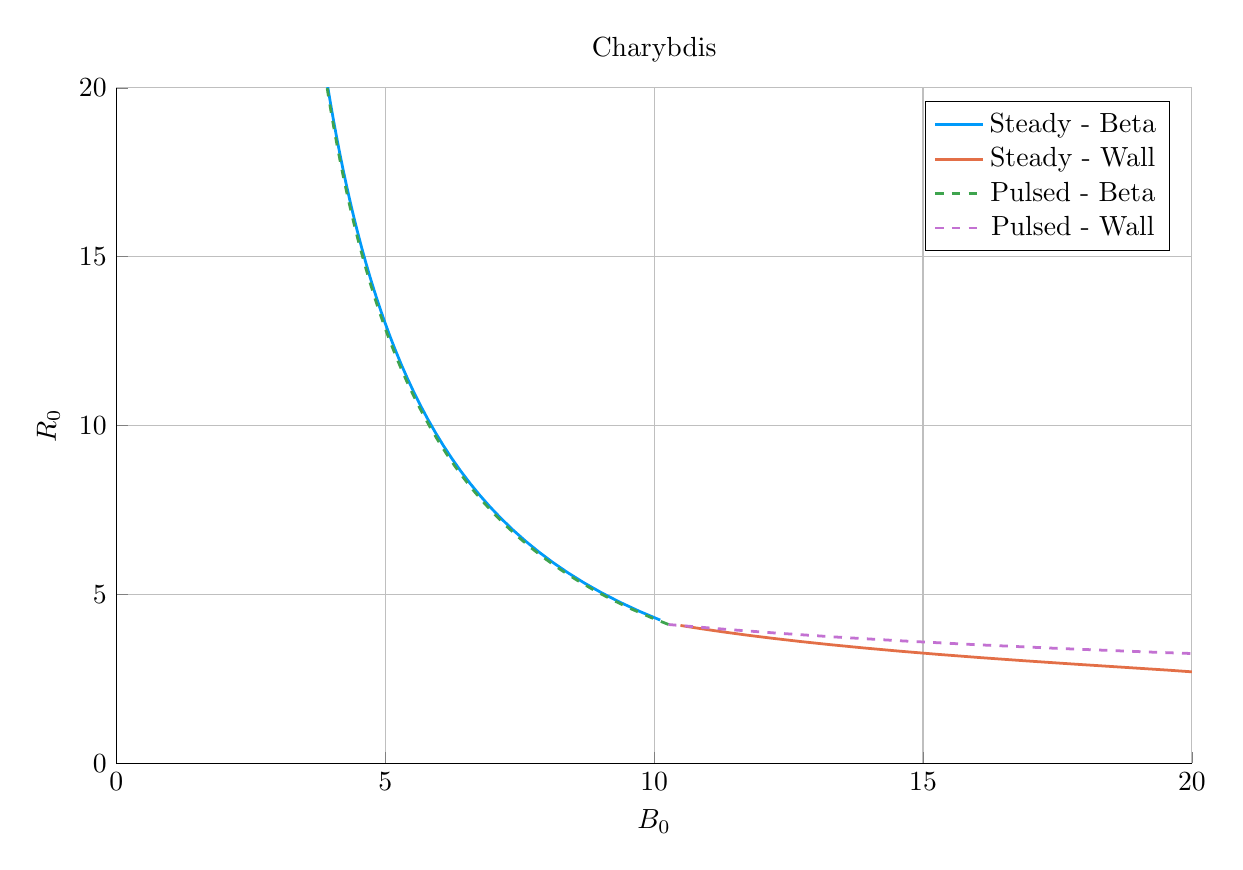
\begin{tikzpicture}[]
\begin{axis}[height = {101.6mm}, ylabel = {${R}_{0}$}, title = {Charybdis}, xmin = {0.0}, xmax = {20.0}, ymax = {20.0}, xlabel = {${B}_{0}$}, {unbounded coords=jump, scaled x ticks = false, xticklabel style={rotate = 0}, xmajorgrids = true, xtick = {0.0,5.0,10.0,15.0,20.0}, xticklabels = {0,5,10,15,20}, xtick align = inside, axis lines* = left, scaled y ticks = false, yticklabel style={rotate = 0}, ymajorgrids = true, ytick = {0.0,5.0,10.0,15.0,20.0}, yticklabels = {0,5,10,15,20}, ytick align = inside, axis lines* = left,     xshift = 0.0mm,
    yshift = 0.0mm,
    axis background/.style={fill={rgb,1:red,1.00000000;green,1.00000000;blue,1.00000000}}
, colorbar style={title=}}, ymin = {0.0}, width = {152.4mm}]\addplot+ [color = {rgb,1:red,0.00000000;green,0.60560316;blue,0.97868012},
draw opacity=1.0,
line width=1,
solid,mark = none,
mark size = 2.0,
mark options = {
    color = {rgb,1:red,0.00000000;green,0.00000000;blue,0.00000000}, draw opacity = 1.0,
    fill = {rgb,1:red,0.00000000;green,0.60560316;blue,0.97868012}, fill opacity = 1.0,
    line width = 1,
    rotate = 0,
    solid
}]coordinates {
(10.112818033153026, 4.241771689478311)
(9.722156888543116, 4.504138117525138)
(9.357875603858393, 4.77497367032698)
(9.017653755630063, 5.054228410858618)
(8.6995124437054, 5.34178832481448)
(8.401566530516865, 5.637594610921002)
(8.122163706328223, 5.941556970897918)
(7.859819415455661, 6.2535750482800845)
(7.613196557650265, 6.5735387749268055)
(7.381088038653343, 6.901328733442317)
(7.162401716104116, 7.236816533350192)
(6.956147367527331, 7.579865198961832)
(6.761425371986388, 7.930329566972662)
(6.577416849463348, 8.28805669191591)
(6.403375044688587, 8.652886257700402)
(6.2386177769852695, 9.02465099355178)
(6.0825208065966905, 9.403177092267818)
(5.934511989185341, 9.788284632344096)
(5.794066116682695, 10.179787994954152)
(5.660700347012839, 10.577496284633074)
(5.533970150598111, 10.981213744847159)
(5.413465705416883, 11.390740170754555)
(5.298808685607224, 11.805871315185586)
(5.189649392059402, 12.226399293085946)
(5.085664187259174, 12.652112975136994)
(4.986553195072601, 13.082798376170517)
(4.892038235455667, 13.518239035062717)
(4.801860966679364, 13.958216385902286)
(4.7157812114040425, 14.402510119861804)
(4.633575445956479, 14.850898537267405)
(4.5550354347559185, 15.303158889428241)
(4.479966994069385, 15.759067709846747)
(4.408188871204256, 16.21840113449116)
(4.33953172691477, 16.680935210866018)
(4.273837210246432, 17.14644619566822)
(4.210957116299974, 17.614710840865197)
(4.15075261849161, 18.085506668079862)
(4.0930935678432965, 18.558612231207235)
(4.037857852672517, 19.03380736722975)
(3.9849308127842145, 19.510873435234036)
(3.9342047029103653, 19.98959354366903)
(3.8855782007091695, 20.46975276591405)
(3.838955955133626, 20.951138344257103)
(3.7942481714200484, 21.433539882408354)
(3.7513702293348077, 21.91674952670236)
(3.710242331663442, 22.400562136158193)
(3.6707891802306123, 22.88477544159215)
(3.6329396770109583, 23.369190193993973)
(3.5966266481325166, 23.853610302391182)
(3.5617865887889004, 24.33784296144382)
(3.5283594272686503, 24.821698769019683)
(3.496288306480746, 25.30499183401733)
(3.465519381509793, 25.787539874702443)
(3.4360016318699595, 26.2691643078435)
(3.4076866872513096, 26.74969032892794)
(3.380528665662031, 27.228946983749)
(3.3544840229690007, 27.706767231660894)
(3.3295114129297314, 28.18298800079238)
(3.3055715568879336, 28.6574502355218)
(3.2826271223788512, 29.129998936506894)
(3.260642607548369, 29.600483215419466)
(3.239584247604666, 30.068756211731234)
(3.2194198921826622, 30.53467533068977)
(3.2001189373344725, 30.998102038032528)
(3.181652227422265, 31.45890197647381)
(3.163991977015565, 31.916944945395528)
(3.1471116955378684, 32.37210489697581)
(3.130986116696265, 32.82425992717794)
(3.115591132350856, 33.27329226186858)
(3.1009037305081053, 33.719088238329654)
(3.0869019371473265, 34.16153828242195)
(3.0735647616124355, 34.600536881650775)
(3.0608721453218655, 35.035982554380354)
};
\addlegendentry{Steady - Beta}
\addplot+ [color = {rgb,1:red,0.88887350;green,0.43564919;blue,0.27812294},
draw opacity=1.0,
line width=1,
solid,mark = none,
mark size = 2.0,
mark options = {
    color = {rgb,1:red,0.00000000;green,0.00000000;blue,0.00000000}, draw opacity = 1.0,
    fill = {rgb,1:red,0.88887350;green,0.43564919;blue,0.27812294}, fill opacity = 1.0,
    line width = 1,
    rotate = 0,
    solid
}]coordinates {
(20.758867641064707, 2.5885674971573294)
(20.346250098246923, 2.6701608818805265)
(19.57104597888471, 2.7580768645580767)
(18.681781921115476, 2.84914579801761)
(17.775790175980152, 2.942053074257325)
(16.896654716492492, 3.036102404206255)
(16.063927450323227, 3.1308756359103893)
(15.285557510665852, 3.226095678435203)
(14.563500533069154, 3.3215674678202314)
(13.896568848875791, 3.417147967307318)
(13.281970890030232, 3.5127292434426214)
(12.716170469467318, 3.6082281475654683)
(12.195372283741088, 3.7035796419955296)
(11.715794270833433, 3.798732281084355)
(11.273815669498969, 3.8936450383948094)
(10.866051794088186, 3.9882850129983627)
(10.489365023931143, 4.08262666943062)
};
\addlegendentry{Steady - Wall}
\addplot+ [color = {rgb,1:red,0.24222430;green,0.64327509;blue,0.30444865},
draw opacity=1.0,
line width=1,
dashed,mark = none,
mark size = 2.0,
mark options = {
    color = {rgb,1:red,0.00000000;green,0.00000000;blue,0.00000000}, draw opacity = 1.0,
    fill = {rgb,1:red,0.24222430;green,0.64327509;blue,0.30444865}, fill opacity = 1.0,
    line width = 1,
    rotate = 0,
    solid
}]coordinates {
(10.26788634689966, 4.1112515557786775)
(9.953967652326213, 4.3094639978912825)
(9.567926244368271, 4.576742787082168)
(9.207974394987358, 4.852707848855866)
(8.871841888699304, 5.137296446755483)
(8.557505525932248, 5.430432251844937)
(8.263156925406376, 5.732025498645217)
(7.9871752024348766, 6.041973183885721)
(7.728103682045175, 6.3601593098028015)
(7.484629973620137, 6.686455168691173)
(7.255568856523303, 7.020719666856628)
(7.039847526735421, 7.362799685753208)
(6.836492834698909, 7.712530477959993)
(6.644620209081183, 8.06973609553486)
(6.463424013335149, 8.43422984818008)
(6.2921691243175495, 8.80581478856818)
(6.13018355681404, 9.184284222105854)
(5.97685198655569, 9.569422237740964)
(5.831610044919842, 9.961004260702955)
(5.693939286027163, 10.358797615092055)
(5.563362729090489, 10.762562105803609)
(5.439440906144732, 11.172050607751359)
(5.321768347746793, 11.587009663771289)
(5.209970453003084, 12.007180084871303)
(5.103700692769835, 12.43229755779498)
(5.002638109938164, 12.862093246958203)
(4.906485077678376, 13.296294396161224)
(4.814965286571576, 13.734624924501638)
(4.727821933804548, 14.176806014771396)
(4.644816091323922, 14.622556692215932)
(4.565725232806084, 15.071594391671503)
(4.490341901840154, 15.523635511246878)
(4.418472505906755, 15.978395950871612)
(4.349936222622964, 16.435591634187325)
(4.284564006352339, 16.89493901242702)
(4.222197684694192, 17.3561555490841)
(4.162689135592264, 17.818960184341037)
(4.105899536872315, 18.283073778386605)
(4.051698680949713, 18.748219532911282)
(3.9999643482627323, 19.214123390225897)
(3.9505817337017928, 19.680514409594025)
(3.903442920928527, 20.147125120523665)
(3.858446400032002, 20.613691852887264)
(3.8154966244515616, 21.079955043879853)
(3.7745036035252744, 21.545659521938795)
(3.7353825273991994, 22.010554767868463)
(3.6980534213689746, 22.47439515350876)
(3.6624408270205375, 22.936940158387063)
(3.62847350780097, 23.397954564874027)
(3.5960841768845415, 23.85720863243935)
(3.565209245407392, 24.314478251672824)
(3.5357885893311605, 24.769545078785413)
(3.5077653333614305, 25.22219665136009)
(3.4810856504959875, 25.672226486155235)
(3.4556985759109375, 26.119434159797105)
(3.4315558340122845, 26.563625373217942)
(3.408611677587535, 27.004612000714285)
(3.3868227380888998, 27.44221212450356)
(3.36614788616562, 27.876250055664674)
(3.3465481016421226, 28.306556342336567)
(3.327986352208224, 28.732967766047434)
(3.3104274769652595, 29.155327355093103)
(3.2938380965241474, 29.573484219331384)
(3.278186482171801, 29.987293796610192)
(3.263442495132517, 30.396617529277517)
(3.2495774839156075, 30.801322953869263)
(3.236564206241785, 31.2012836153002)
(3.224376752844934, 31.596379002720997)
(3.212990475972638, 31.98649447963656)
(3.2023819222517877, 32.371521208907616)
(3.192528769611062, 32.751356073231776)
(3.1834097679780142, 33.12590159165121)
(3.1750046834890777, 33.49506583261046)
(3.1672942459724482, 33.8587623240416)
};
\addlegendentry{Pulsed - Beta}
\addplot+ [color = {rgb,1:red,0.76444018;green,0.44411178;blue,0.82429754},
draw opacity=1.0,
line width=1,
dashed,mark = none,
mark size = 2.0,
mark options = {
    color = {rgb,1:red,0.00000000;green,0.00000000;blue,0.00000000}, draw opacity = 1.0,
    fill = {rgb,1:red,0.76444018;green,0.44411178;blue,0.82429754}, fill opacity = 1.0,
    line width = 1,
    rotate = 0,
    solid
}]coordinates {
(48.990476413653056, 2.408463256282958)
(42.83950920694117, 2.5157944044289065)
(37.687790427214495, 2.623911121514849)
(33.33937742845888, 2.732773154793489)
(29.64296398154308, 2.8423415573543895)
(26.48039367255613, 2.9525785265823425)
(23.758442882319894, 3.0634472709719978)
(21.402860298405816, 3.174911900538905)
(19.353987387634486, 3.2869373368800954)
(17.563502020363714, 3.3994892396762393)
(15.991970371213752, 3.512533946790301)
(14.606987499719377, 3.6260384258753686)
(13.381751501116137, 3.7399702354868722)
(12.293960329570087, 3.854297494171075)
(11.32495111804522, 3.9689888562032056)
(10.459023415380802, 4.084013492866982)
(10.26788634689966, 4.1112515557786775)
};
\addlegendentry{Pulsed - Wall}
\end{axis}

\end{tikzpicture}

    \end{adjustbox}
        \caption{Charybdis Reactor}
    \end{subfigure}
    \hfill
    \begin{subfigure}[t]{0.45\textwidth}
        \centering
    \begin{adjustbox}{width=\textwidth}
      \Large
      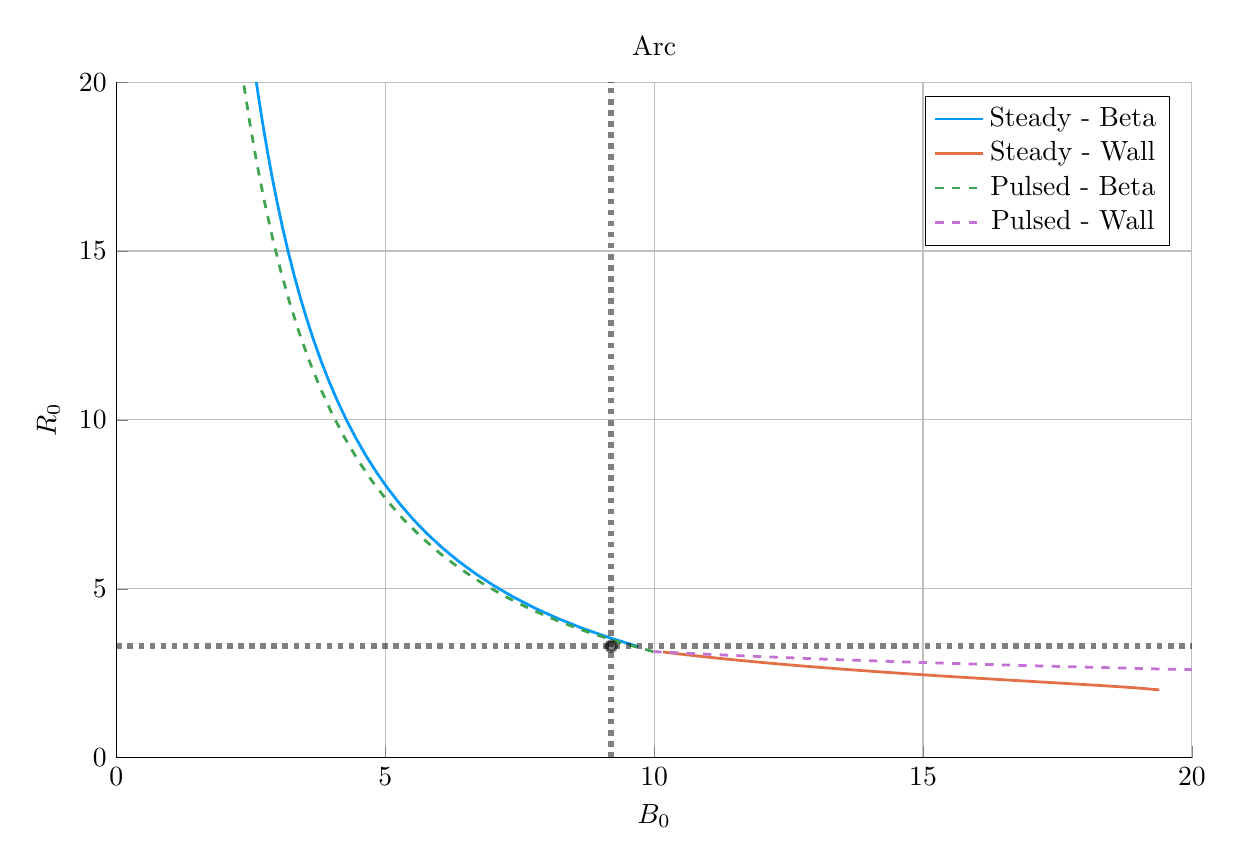
\begin{tikzpicture}[]
\begin{axis}[height = {101.6mm}, ylabel = {${R}_{0}$}, title = {Arc}, xmin = {0.0}, xmax = {20.0}, ymax = {20.0}, xlabel = {${B}_{0}$}, {unbounded coords=jump, scaled x ticks = false, xticklabel style={rotate = 0}, xmajorgrids = true, xtick = {0.0,5.0,10.0,15.0,20.0}, xticklabels = {0,5,10,15,20}, xtick align = inside, axis lines* = left, scaled y ticks = false, yticklabel style={rotate = 0}, ymajorgrids = true, ytick = {0.0,5.0,10.0,15.0,20.0}, yticklabels = {0,5,10,15,20}, ytick align = inside, axis lines* = left,     xshift = 0.0mm,
    yshift = 0.0mm,
    axis background/.style={fill={rgb,1:red,1.00000000;green,1.00000000;blue,1.00000000}}
, colorbar style={title=}}, ymin = {0.0}, width = {152.4mm}]\addplot+ [color = {rgb,1:red,0.00000000;green,0.60560316;blue,0.97868012},
draw opacity=1.0,
line width=1,
solid,mark = none,
mark size = 2.0,
mark options = {
    color = {rgb,1:red,0.00000000;green,0.00000000;blue,0.00000000}, draw opacity = 1.0,
    fill = {rgb,1:red,0.00000000;green,0.60560316;blue,0.97868012}, fill opacity = 1.0,
    line width = 1,
    rotate = 0,
    solid
}]coordinates {
(9.701206080853105, 3.2904233285656006)
(9.162315904693079, 3.553631706046861)
(8.664301107137337, 3.8315748016260343)
(8.203576462497304, 4.124583886864978)
(7.776718537485166, 4.433072975674755)
(7.380720231870917, 4.75741949036414)
(7.012886014999712, 5.097987291342331)
(6.670795005901889, 5.4551257000070565)
(6.352268997292712, 5.829168567645448)
(6.055344682097163, 6.220433393277178)
(5.778249464564785, 6.629220493040615)
(5.519380338856715, 7.05581222339423)
(5.2772854007125325, 7.500472260074458)
(5.050647625972996, 7.963444934423652)
(4.838270606140816, 8.444954628380609)
(4.639065978019038, 8.94520522910952)
(4.4520423235376105, 9.464379643936518)
(4.276295348572609, 10.002639375969222)
(4.110999177018484, 10.56012416048812)
(3.9553986195015125, 11.136951661929974)
(3.8088022956698633, 11.733217231026282)
(3.6705765055641186, 12.34899372141899)
(3.54013975965751, 12.984331364849716)
(3.4169578891619192, 13.639257703809928)
(3.30053966845824, 14.313777580345645)
(3.1904328903033052, 15.007873179535935)
(3.086220842019516, 15.721504126002731)
(2.9875191373772063, 16.45460763166718)
(2.8939728644914635, 17.207098692842226)
(2.8052540149097247, 17.97887033463821)
(2.7210591632720242, 18.7697939005645)
(2.6411073705789065, 19.579719385129263)
(2.565138287279709, 20.40847580717446)
(2.492910435164382, 21.255871621630877)
(2.4241996494611984, 22.12169516733927)
(2.3587976646588236, 23.0057151485579)
(2.296510829425685, 23.907681147764652)
(2.237158937627476, 24.827324167354146)
(2.180574163874242, 25.764357197843207)
(2.126600093288366, 26.71847581021091)
(2.075090836295778, 27.689358770027713)
(2.0259102202234582, 28.676668671060817)
(1.978931050353818, 29.68005258608471)
(1.9340344338545452, 30.69914273267572)
(1.8911091606836798, 31.733557151818793)
(1.8500511361739687, 32.78290039722107)
(1.8107628605384507, 33.846764233283025)
(1.773152951016952, 34.92472833975579)
(1.7371357028100902, 36.01636102117257)
(1.7026306853269466, 37.121219919229354)
(1.6695623706125668, 38.23885272635799)
(1.6378597911249178, 39.368797898817405)
(1.607456224302725, 40.51058536770822)
(1.5782889016090462, 41.663737246396295)
(1.5502987399539199, 42.82776853291479)
(1.5234300935954943, 44.00218780599217)
(1.4976305247952577, 45.18649791343829)
(1.4728505916614916, 46.38019665170201)
(1.4490436517578602, 47.58277743549339)
(1.4261656801829077, 48.79372995643627)
};
\addlegendentry{Steady - Beta}
\addplot+ [color = {rgb,1:red,0.88887350;green,0.43564919;blue,0.27812294},
draw opacity=1.0,
line width=1,
solid,mark = none,
mark size = 2.0,
mark options = {
    color = {rgb,1:red,0.00000000;green,0.00000000;blue,0.00000000}, draw opacity = 1.0,
    fill = {rgb,1:red,0.88887350;green,0.43564919;blue,0.27812294}, fill opacity = 1.0,
    line width = 1,
    rotate = 0,
    solid
}]coordinates {
(19.394007482712425, 2.006855814841082)
(18.932196567189358, 2.070220226465634)
(18.296989378345195, 2.1362327099649083)
(17.587029315408756, 2.2039322514902886)
(16.847882407994106, 2.272885741349308)
(16.111374502564406, 2.3427307443133163)
(15.396027314547156, 2.4132115621474344)
(14.710952688793137, 2.484165095168367)
(14.06168447794857, 2.555449485048069)
(13.450465418483889, 2.6269568263788754)
(12.877644538645335, 2.6986005527245354)
(12.342394470642008, 2.7703103261458715)
(11.843182246608265, 2.8420284550528074)
(11.376441269625893, 2.9137564749008216)
(10.944966372727551, 2.985307257194073)
(10.541663878705513, 3.056795384934831)
(10.165908182236457, 3.128148092221394)
};
\addlegendentry{Steady - Wall}
\addplot+ [color = {rgb,1:red,0.24222430;green,0.64327509;blue,0.30444865},
draw opacity=1.0,
line width=1,
dashed,mark = none,
mark size = 2.0,
mark options = {
    color = {rgb,1:red,0.00000000;green,0.00000000;blue,0.00000000}, draw opacity = 1.0,
    fill = {rgb,1:red,0.24222430;green,0.64327509;blue,0.30444865}, fill opacity = 1.0,
    line width = 1,
    rotate = 0,
    solid
}]coordinates {
(9.980483622051658, 3.1402982942956537)
(9.392786903460065, 3.3984668375583613)
(8.79273598103983, 3.7029994270206985)
(8.23820290909994, 4.029752381934837)
(7.725182218401588, 4.380005330007902)
(7.250078106370205, 4.755088191072525)
(6.80965553466646, 5.15638156809462)
(6.400998063035608, 5.585317075247801)
(6.0214713600430425, 6.043377623224966)
(5.668691517461799, 6.532097691007738)
(5.340497445229901, 7.053063624618788)
(5.034926745580058, 7.607914017422467)
(4.750194564008521, 8.198340243900201)
(4.484674995755211, 8.826087240213646)
(4.236884692979903, 9.49295465115087)
(4.00546837264544, 10.200798495308337)
(3.7891859704718387, 10.951533539957822)
(3.5869012239550364, 11.747136625739826)
(3.3975714987448393, 12.589651241396528)
(3.2202386987489797, 13.481193723261853)
(3.0540211220494466, 14.423961547290066)
(2.8981061427709687, 15.420244298711943)
(2.7517436139566023, 16.472438053930638)
(2.6142398986781377, 17.58306410230943)
(2.4849524463010138, 18.754793188384546)
(2.363284838174807, 19.990476791576892)
(2.248682232019848, 21.293187416028662)
(2.140627136740878, 22.666270490916787)
(2.038635448877246, 24.113411362836906)
(1.9422526775794744, 25.638722123308433)
(1.8510502754751532, 27.246854857488287)
(1.7646219756564088, 28.94315065234289)
(1.6825800061969869, 30.73383791051506)
(1.6045510059627948, 32.62630011975996)
(1.53017138625397, 34.629443897654504)
(1.4590817483192686, 36.754215952550474)
(1.3909197311384796, 39.01434852880224)
(1.3253102336217724, 41.42746903285954)
(1.261851128383913, 44.01681696754988)
(1.20009089049112, 46.81403058684408)
(1.1394908096975784, 49.863950342519615)
};
\addlegendentry{Pulsed - Beta}
\addplot+ [color = {rgb,1:red,0.76444018;green,0.44411178;blue,0.82429754},
draw opacity=1.0,
line width=1,
dashed,mark = none,
mark size = 2.0,
mark options = {
    color = {rgb,1:red,0.00000000;green,0.00000000;blue,0.00000000}, draw opacity = 1.0,
    fill = {rgb,1:red,0.76444018;green,0.44411178;blue,0.82429754}, fill opacity = 1.0,
    line width = 1,
    rotate = 0,
    solid
}]coordinates {
(29.27715761652869, 2.3448804182939873)
(25.4410619834368, 2.4377937236066716)
(22.158819835998365, 2.5322208586485804)
(19.342453256965573, 2.628163744265164)
(16.919364280634177, 2.7256238396687067)
(14.829378672669455, 2.8246020951898183)
(13.022412368922526, 2.9250989082568273)
(11.456617692058645, 3.0271140820266207)
(10.096901921254785, 3.1306467862637533)
(9.980483622051658, 3.1402982942956537)
};
\addlegendentry{Pulsed - Wall}
\addplot+ [color = {rgb,1:red,0.00000000;green,0.00000000;blue,0.00000000},
draw opacity=0.5,
line width=2,
dotted,mark = none,
mark size = 2.0,
mark options = {
    color = {rgb,1:red,0.00000000;green,0.00000000;blue,0.00000000}, draw opacity = 0.5,
    fill = {rgb,1:red,0.00000000;green,0.00000000;blue,0.00000000}, fill opacity = 0.5,
    line width = 1,
    rotate = 0,
    solid
},forget plot]coordinates {
(0.0, 3.3)
(20.0, 3.3)
};
\addplot+ [color = {rgb,1:red,0.00000000;green,0.00000000;blue,0.00000000},
draw opacity=0.5,
line width=2,
dotted,mark = none,
mark size = 2.0,
mark options = {
    color = {rgb,1:red,0.00000000;green,0.00000000;blue,0.00000000}, draw opacity = 0.5,
    fill = {rgb,1:red,0.00000000;green,0.00000000;blue,0.00000000}, fill opacity = 0.5,
    line width = 1,
    rotate = 0,
    solid
},forget plot]coordinates {
(9.2, 0.0)
(9.2, 20.0)
};
\addplot+[draw=none, color = {rgb,1:red,0.00000000;green,0.00000000;blue,0.00000000},
draw opacity=0.5,
line width=0,
solid,mark = *,
mark size = 2.0,
mark options = {
    color = {rgb,1:red,0.00000000;green,0.00000000;blue,0.00000000}, draw opacity = 0.5,
    fill = {rgb,1:red,0.00000000;green,0.00000000;blue,0.00000000}, fill opacity = 0.5,
    line width = 1,
    rotate = 0,
    solid
},forget plot] coordinates {
(9.2, 3.3)
};
\end{axis}

\end{tikzpicture}

    \end{adjustbox}
        \caption{Arc Reactor}
    \end{subfigure}
    \hfill \hfill ~\\ ~\\ ~\\
    \caption{Steady State Prototype Comparison} ~\\
    \label{fig:charybdis}
\end{figure*}

\begin{table}[h!]
\centering  
\caption{Charybdis Variables}
\hfill
\begin{subtable}[t]{0.4\textwidth}
\centering  
\caption{Input Variables} ~\\
\begin{tabular}{ c|c } 

Input            & Value           \\
\hline
$H$              & 1.7              \\
$Q$              & 25.0             \\
$N_{G}$          & 0.9              \\
$\epsilon$       & 0.3              \\
$\kappa_{95}$    & 1.8              \\
$\delta_{95}$    & 0.35             \\
$\nu_{n}$        & 0.4              \\
$\nu_{T}$        & 1.1              \\
$l_{i}$          & 0.5579         \\
$A$              & 2.5              \\
$Z_{eff}$        & 1.75             \\
$f_{D}$          & 0.9              \\
$\tau_{FT}$      & 1.6e9            \\
$B_{CS}$         & 12.0             \\

\end{tabular}
\end{subtable}
\hfill
\begin{subtable}[t]{0.5\textwidth}
\centering  
\caption{Output Variables} ~\\
\begin{tabular}{ c|c } 

Output           & Value       \\
\hline
$R_{0}$          & 4.13            \\
$B_{0}$          & 10.28            \\
$I_{P}$          & 8.98            \\
$\overline n$    & 1.47            \\
$\overline T$    & 15.81           \\
$\beta_{N}$       & 0.028            \\
$q_{95}$         & 6.089            \\
$P_{W}$          & 3.003            \\
$f_{BS}$         & 0.723           \\
$f_{CD}$         & 0.277           \\
$f_{IN}$         & 0.0              \\
$\volume$         & 225.5            \\
$P_{F}$          & 1294           \\
$\eta_{CD}$      & 0.291           \\

\end{tabular}
\end{subtable}
\hfill
\hfill
\end{table}

\newpage 

\subsection{Pinning down Proteus}

The pulsed twin reactor, Proteus, highlights the effects o f a high field central solenoid. When compared to the Pulsed Demo design, the $R_0$ -- $B_0$ curves look far more favorable -- i.e. each machine built at a certain magnet strength would be more compact (and cheaper). An interesting facet of Proteus is that it exhibits all three used limits: kink, beta, and wall.

\begin{figure*}[h!]
    \centering
    \hfill 
    \begin{subfigure}[t]{0.45\textwidth}
        \centering
    \begin{adjustbox}{width=\textwidth}
      \Large
      \begin{tikzpicture}[]
\begin{axis}[height = {101.6mm}, ylabel = {${R}_{0}$}, title = {Proteus}, xmin = {0.0}, xmax = {20.0}, ymax = {20.0}, xlabel = {${B}_{0}$}, {unbounded coords=jump, scaled x ticks = false, xticklabel style={rotate = 0}, xmajorgrids = true, xtick = {0.0,5.0,10.0,15.0,20.0}, xticklabels = {0,5,10,15,20}, xtick align = inside, axis lines* = left, scaled y ticks = false, yticklabel style={rotate = 0}, ymajorgrids = true, ytick = {0.0,5.0,10.0,15.0,20.0}, yticklabels = {0,5,10,15,20}, ytick align = inside, axis lines* = left,     xshift = 0.0mm,
    yshift = 0.0mm,
    axis background/.style={fill={rgb,1:red,1.00000000;green,1.00000000;blue,1.00000000}}
, colorbar style={title=}}, ymin = {0.0}, width = {152.4mm}]\addplot+ [color = {rgb,1:red,0.00000000;green,0.60560316;blue,0.97868012},
draw opacity=1.0,
line width=1,
solid,mark = none,
mark size = 2.0,
mark options = {
    color = {rgb,1:red,0.00000000;green,0.00000000;blue,0.00000000}, draw opacity = 1.0,
    fill = {rgb,1:red,0.00000000;green,0.60560316;blue,0.97868012}, fill opacity = 1.0,
    line width = 1,
    rotate = 0,
    solid
}]coordinates {
(4.658732060637907, 15.19267920719026)
(4.211109766361548, 13.257359890602805)
(3.9293920326356777, 11.874737313931622)
(3.7651903683456465, 10.866007699416029)
(3.6776039543745567, 10.103021459180615)
(3.6402437753208394, 9.505760636119051)
(3.6366994671255806, 9.024418756735512)
(3.656621534643579, 8.627122931627166)
(3.693300156736026, 8.29276379316033)
(3.7422515017241134, 8.006879676976913)
(3.865532743079537, 7.5424484228595015)
(3.936096932264377, 7.350942552250971)
(4.010907188015084, 7.180521653028847)
(4.089072356933184, 7.027918062531758)
(4.169903401491354, 6.8905526178616)
(4.252857906625248, 6.7663586425757165)
(4.337501757261618, 6.653657691692545)
(4.42348218754058, 6.551070097987566)
(4.5983381267510195, 6.371833566535418)
(4.686766232902671, 6.29340795554276)
(4.775618142770625, 6.221477142908907)
(4.864743502376605, 6.155442914152805)
(4.927312314219091, 6.1123879686673135)
};
\addlegendentry{Pulsed - Kink}
\addplot+ [color = {rgb,1:red,0.88887350;green,0.43564919;blue,0.27812294},
draw opacity=1.0,
line width=1,
solid,mark = none,
mark size = 2.0,
mark options = {
    color = {rgb,1:red,0.00000000;green,0.00000000;blue,0.00000000}, draw opacity = 1.0,
    fill = {rgb,1:red,0.88887350;green,0.43564919;blue,0.27812294}, fill opacity = 1.0,
    line width = 1,
    rotate = 0,
    solid
}]coordinates {
(4.927312314219091, 6.1123879686673135)
(4.984545814413324, 6.09581207033949)
(5.17452482724068, 6.0447147858623)
(5.362091669637646, 5.999934523234248)
(5.54700293215903, 5.961033646850443)
(5.729042482638278, 5.92761240871646)
(5.908022832274664, 5.899302777254819)
(6.083785777786694, 5.87576371038825)
(6.256202341425288, 5.85667756374391)
(6.324169421042356, 5.850226299362774)
};
\addlegendentry{Pulsed - Beta}
\addplot+ [color = {rgb,1:red,0.24222430;green,0.64327509;blue,0.30444865},
draw opacity=1.0,
line width=1,
solid,mark = none,
mark size = 2.0,
mark options = {
    color = {rgb,1:red,0.00000000;green,0.00000000;blue,0.00000000}, draw opacity = 1.0,
    fill = {rgb,1:red,0.24222430;green,0.64327509;blue,0.30444865}, fill opacity = 1.0,
    line width = 1,
    rotate = 0,
    solid
}]coordinates {
(6.324169421042356, 5.850226299362774)
(6.727338549778396, 5.88388315153579)
(7.320469048424473, 5.950696360836003)
(7.835746509376305, 6.026778469060774)
(8.290245520072391, 6.109137751468495)
(8.696162676727877, 6.195913809142839)
(9.0624397222742, 6.285887257774413)
(9.395798186463841, 6.3782240354403505)
(9.701405747258567, 6.472333393687546)
(10.244760202900984, 6.664256338261126)
(10.930275827723788, 6.957604003970967)
(11.131878682735255, 7.056189303396245)
(11.50278450645086, 7.253945523825199)
(11.83715172742864, 7.452031096358636)
(11.992609772603878, 7.551070724623068)
(12.141110720831467, 7.650057379146056)
};
\addlegendentry{Pulsed - Wall}
\end{axis}

\end{tikzpicture}

    \end{adjustbox}
        \caption{Proteus Reactor}
    \end{subfigure}
    \hfill
    \begin{subfigure}[t]{0.45\textwidth}
        \centering
    \begin{adjustbox}{width=\textwidth}
      \Large
      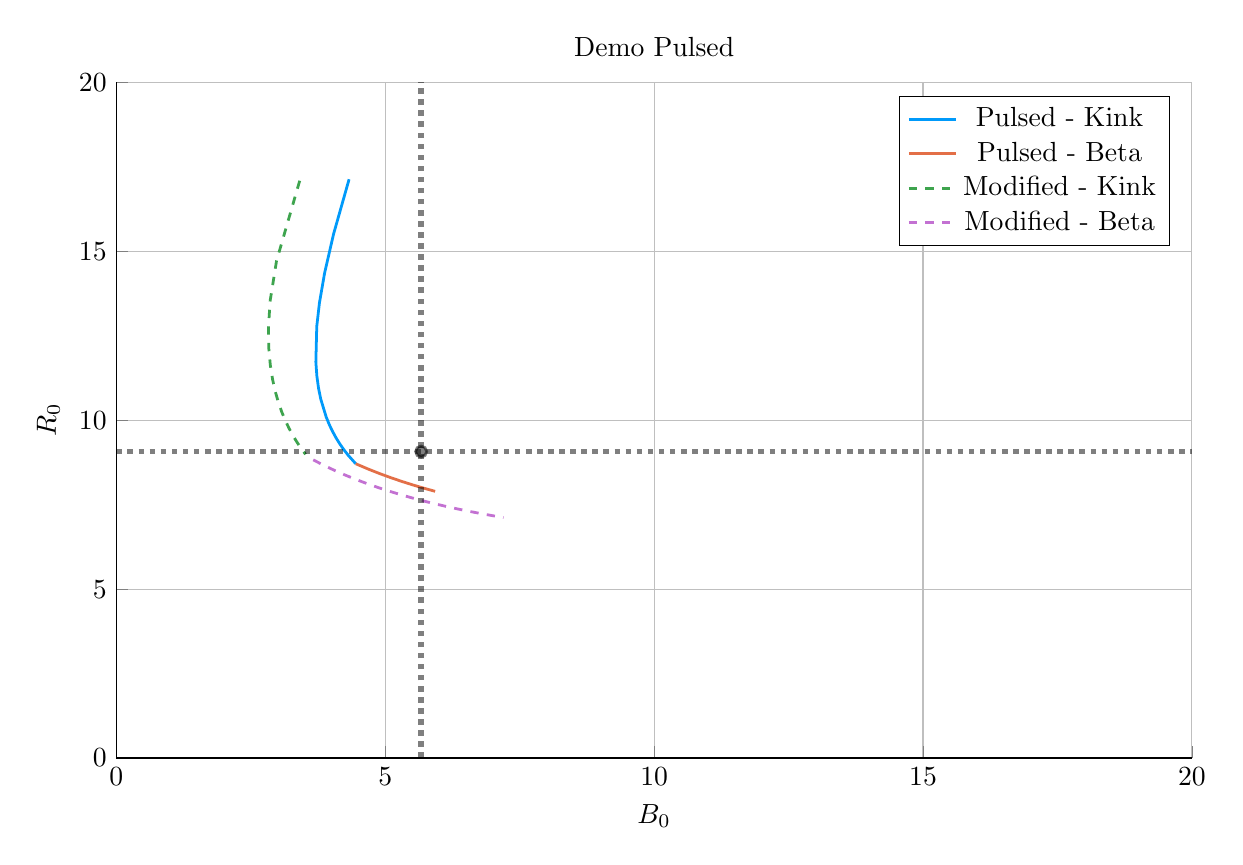
\begin{tikzpicture}[]
\begin{axis}[height = {101.6mm}, ylabel = {${R}_{0}$}, title = {Demo Pulsed}, xmin = {0.0}, xmax = {20.0}, ymax = {20.0}, xlabel = {${B}_{0}$}, {unbounded coords=jump, scaled x ticks = false, xticklabel style={rotate = 0}, xmajorgrids = true, xtick = {0.0,5.0,10.0,15.0,20.0}, xticklabels = {0,5,10,15,20}, xtick align = inside, axis lines* = left, scaled y ticks = false, yticklabel style={rotate = 0}, ymajorgrids = true, ytick = {0.0,5.0,10.0,15.0,20.0}, yticklabels = {0,5,10,15,20}, ytick align = inside, axis lines* = left,     xshift = 0.0mm,
    yshift = 0.0mm,
    axis background/.style={fill={rgb,1:red,1.00000000;green,1.00000000;blue,1.00000000}}
, colorbar style={title=}}, ymin = {0.0}, width = {152.4mm}]\addplot+ [color = {rgb,1:red,0.00000000;green,0.60560316;blue,0.97868012},
draw opacity=1.0,
line width=1,
solid,mark = none,
mark size = 2.0,
mark options = {
    color = {rgb,1:red,0.00000000;green,0.00000000;blue,0.00000000}, draw opacity = 1.0,
    fill = {rgb,1:red,0.00000000;green,0.60560316;blue,0.97868012}, fill opacity = 1.0,
    line width = 1,
    rotate = 0,
    solid
}]coordinates {
(4.327031075670194, 17.134796748649162)
(4.038214026054326, 15.511755022601415)
(3.8713719163129245, 14.355562963913712)
(3.7758613845615545, 13.476675762289453)
(3.7257856761317214, 12.778294295391971)
(3.7090473695925437, 11.723065749829066)
(3.727711597554826, 11.30970201784727)
(3.7586131667481433, 10.94971275897184)
(3.799052518631718, 10.632190690377048)
(3.901290136389271, 10.09455415135144)
(3.960577465316514, 9.863813619410237)
(4.0241209645210345, 9.653307397969705)
(4.0912717805663785, 9.460162902699798)
(4.161514602943343, 9.28206292757184)
(4.2344343960723005, 9.117114543572253)
(4.309692554546368, 8.963753917462126)
(4.450417240491067, 8.712493965092264)
};
\addlegendentry{Pulsed - Kink}
\addplot+ [color = {rgb,1:red,0.88887350;green,0.43564919;blue,0.27812294},
draw opacity=1.0,
line width=1,
solid,mark = none,
mark size = 2.0,
mark options = {
    color = {rgb,1:red,0.00000000;green,0.00000000;blue,0.00000000}, draw opacity = 1.0,
    fill = {rgb,1:red,0.88887350;green,0.43564919;blue,0.27812294}, fill opacity = 1.0,
    line width = 1,
    rotate = 0,
    solid
}]coordinates {
(4.450417240491067, 8.712493965092264)
(4.490148631384312, 8.684308742646298)
(4.692490181445514, 8.547262773806349)
(4.8960344619053355, 8.41947837460442)
(5.100651132702229, 8.30014929484307)
(5.306202822090688, 8.188581738801314)
(5.512545696627038, 8.084175191078112)
(5.719530043226767, 7.986407002697611)
(5.927000883375481, 7.894819882619234)
};
\addlegendentry{Pulsed - Beta}
\addplot+ [color = {rgb,1:red,0.24222430;green,0.64327509;blue,0.30444865},
draw opacity=1.0,
line width=1,
dashed,mark = none,
mark size = 2.0,
mark options = {
    color = {rgb,1:red,0.00000000;green,0.00000000;blue,0.00000000}, draw opacity = 1.0,
    fill = {rgb,1:red,0.24222430;green,0.64327509;blue,0.30444865}, fill opacity = 1.0,
    line width = 1,
    rotate = 0,
    solid
}]coordinates {
(3.4087424183072135, 17.090884129081292)
(2.977074181068944, 14.713048632784332)
(2.8592500074202523, 13.541171522519205)
(2.827199220063259, 12.740024138753894)
(2.8339789008667826, 12.12574468151967)
(2.862412302880871, 11.626187613249266)
(2.9044598258085443, 11.205091848948229)
(2.95577893007882, 10.841432203317366)
(3.0137895352525907, 10.521822649209419)
(3.076849710218805, 10.23716073884787)
(3.1438583711612704, 9.980947801083442)
(3.214045733980633, 9.748367275345563)
(3.2868548955983727, 9.535742205343247)
(3.361871149981842, 9.340197658526863)
(3.4387778750377818, 9.15944098345979)
(3.5173279629378453, 8.991613349767409)
};
\addlegendentry{Modified - Kink}
\addplot+ [color = {rgb,1:red,0.76444018;green,0.44411178;blue,0.82429754},
draw opacity=1.0,
line width=1,
dashed,mark = none,
mark size = 2.0,
mark options = {
    color = {rgb,1:red,0.00000000;green,0.00000000;blue,0.00000000}, draw opacity = 1.0,
    fill = {rgb,1:red,0.76444018;green,0.44411178;blue,0.82429754}, fill opacity = 1.0,
    line width = 1,
    rotate = 0,
    solid
}]coordinates {
(3.6607028750648505, 8.825949645171955)
(3.8574448036470477, 8.664618827122876)
(4.056375867871351, 8.51434867582932)
(4.257366397480293, 8.374075613831488)
(4.460279103534801, 8.242896218794312)
(4.664969389370631, 8.12003771613466)
(4.871285596007394, 8.004834914067093)
(5.07906923307514, 7.896711937521184)
(5.288155233306219, 7.795167587687744)
(5.498372259673351, 7.699763475973523)
(5.709543087166185, 7.610114306522102)
(5.921485076209294, 7.525879840414137)
(6.134010749367255, 7.446758190646709)
(6.346928478632384, 7.372480180910637)
(6.560043285872518, 7.302804563889649)
(6.773157754368795, 7.237513941672651)
(6.986073044284746, 7.176411266758267)
(7.198590001107076, 7.119316828230052)
};
\addlegendentry{Modified - Beta}
\addplot+ [color = {rgb,1:red,0.00000000;green,0.00000000;blue,0.00000000},
draw opacity=0.5,
line width=2,
dotted,mark = none,
mark size = 2.0,
mark options = {
    color = {rgb,1:red,0.00000000;green,0.00000000;blue,0.00000000}, draw opacity = 0.5,
    fill = {rgb,1:red,0.00000000;green,0.00000000;blue,0.00000000}, fill opacity = 0.5,
    line width = 1,
    rotate = 0,
    solid
},forget plot]coordinates {
(0.0, 9.072)
(20.0, 9.072)
};
\addplot+ [color = {rgb,1:red,0.00000000;green,0.00000000;blue,0.00000000},
draw opacity=0.5,
line width=2,
dotted,mark = none,
mark size = 2.0,
mark options = {
    color = {rgb,1:red,0.00000000;green,0.00000000;blue,0.00000000}, draw opacity = 0.5,
    fill = {rgb,1:red,0.00000000;green,0.00000000;blue,0.00000000}, fill opacity = 0.5,
    line width = 1,
    rotate = 0,
    solid
},forget plot]coordinates {
(5.667, 0.0)
(5.667, 20.0)
};
\addplot+[draw=none, color = {rgb,1:red,0.00000000;green,0.00000000;blue,0.00000000},
draw opacity=0.5,
line width=0,
solid,mark = *,
mark size = 2.0,
mark options = {
    color = {rgb,1:red,0.00000000;green,0.00000000;blue,0.00000000}, draw opacity = 0.5,
    fill = {rgb,1:red,0.00000000;green,0.00000000;blue,0.00000000}, fill opacity = 0.5,
    line width = 1,
    rotate = 0,
    solid
},forget plot] coordinates {
(5.667, 9.072)
};
\end{axis}

\end{tikzpicture}

    \end{adjustbox}
        \caption{Demo Pulsed Reactor}
    \end{subfigure}
    \hfill \hfill ~\\ ~\\ ~\\
    \caption{Pulsed Prototype Comparison} ~\\
\end{figure*}

\begin{table}[h!]
\centering  
\caption{Proteus Variables}
\hfill
\begin{subtable}[t]{0.4\textwidth}
\centering  
\caption{Input Variables} ~\\
\begin{tabular}{ c|c } 

Input            & Value           \\
\hline
$H$              & 1.0              \\
$Q$              & 25.0             \\
$N_{G}$          & 0.9              \\
$\epsilon$       & 0.3              \\
$\kappa_{95}$    & 1.8              \\
$\delta_{95}$    & 0.35             \\
$\nu_{n}$        & 0.4              \\
$\nu_{T}$        & 1.1              \\
$l_{i}$          & 0.6328         \\
$A$              & 2.5              \\
$Z_{eff}$        & 1.75             \\
$f_{D}$          & 0.9              \\
$\tau_{FT}$      & 7200           \\
$B_{CS}$         & 20.0             \\

\end{tabular}
\end{subtable}
\hfill
\begin{subtable}[t]{0.5\textwidth}
\centering  
\caption{Output Variables} ~\\
\begin{tabular}{ c|c } 

Output           & Value       \\
\hline
$R_{0}$          & 6.11             \\
$B_{0}$          & 4.93            \\
$I_{P}$          & 15.54            \\
$\overline n$    & 1.16            \\
$\overline T$    & 11.25            \\
$\beta_{N}$       & 0.028            \\
$q_{95}$         & 2.5              \\
$P_{W}$          & 1.763            \\
$f_{BS}$         & 0.2675           \\
$f_{CD}$         & 0.0              \\
$f_{IN}$         & 0.7325           \\
$\volume$         & 732.6            \\
$P_{F}$          & 1667           \\
$\eta_{CD}$      & 0.0              \\

\end{tabular}
\end{subtable}
\hfill
\hfill
\end{table}

\section{Learning from the Data}

Now that the model has been properly vetted and prototypes designed, we can explore how pulsed and steady-state tokamaks scale. Fitting with the Dickens theme, there will be three mostly independent results. The first result will explore how to minimize costs for a reactor by choosing optimum design points. The next will be an argument for how to properly utilize the HTS magnet technology in component design. Lastly, we will take a cursory look at the other parameters capable of lowering machine costs.

\subsection{Picking a Design Point}

With more than twenty design parameters, finding the most efficient reactor is a fool's errand. Intuition building aside, finding good reactors becomes much more feasible when only focusing on floating variables -- i.e. when keeping fixed variables constant. This method, for example, is how all the $R_0$ -- $B_0$ curves have been produced this chapter. Once these curves are produced, it is up to the user to choose which reactor on them to build. However, the guiding metric usually involves lowering some cost, either: capital cost or cost-per-watt.

Regardless of reactor type, most efficient tokamaks operate near the beta limit -- where plasma pressure is greatest. Besides being a regime highly sensitive to magnetic field strength, the beta limit is a constraint that occurs on every reactor (seen by the authors). This beta limit is usually nested between the kink limit to lower $B_0$ values and wall loading to higher ones. Understanding these regimes is the first step towards building an intuition favoring efficient machines.

\begin{figure}
\centering
\begin{adjustbox}{width=0.75\textwidth}
	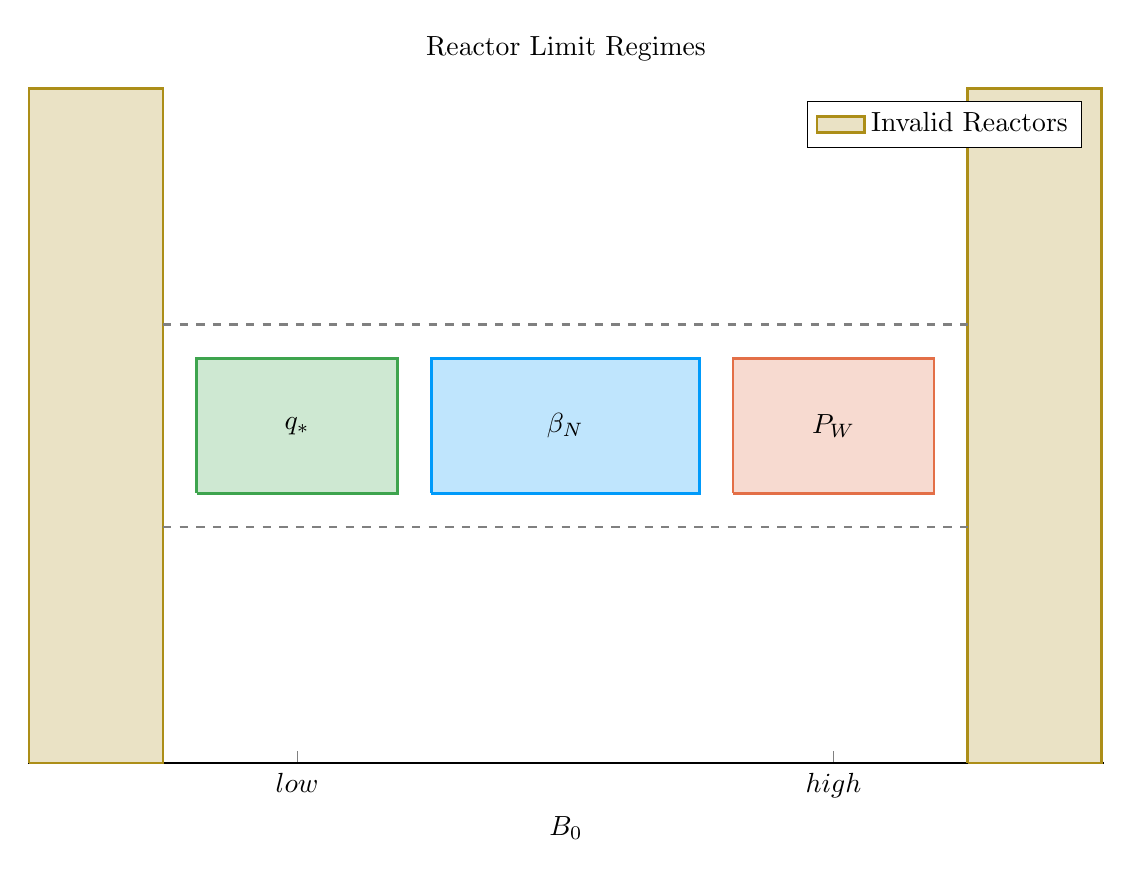
\begin{tikzpicture}[]
\begin{axis}[height = {101.6mm}, ylabel = {}, title = {Reactor Limit Regimes}, xmin = {-0.005}, xmax = {8.015}, ymax = {1.0015}, xlabel = {$B_0$}, {unbounded coords=jump, scaled x ticks = false, xticklabel style={rotate = 0}, xmajorgrids = false, xtick = {2,6}, xticklabels = {$low$,$high$}, xtick align = inside, axis lines* = left, scaled y ticks = false, yticklabel style={rotate = 0}, ymajorticks=false, ymajorgrids = false, axis lines* = left,     xshift = 0.0mm,
    yshift = 0.0mm,
    axis background/.style={fill={rgb,1:red,1.00000000;green,1.00000000;blue,1.00000000}}
, colorbar style={title=}}, ymin = {0}, width = {152.4mm}]\addplot+ [color = {rgb,1:red,0.67554396;green,0.55566233;blue,0.09423434},
draw opacity=1.0,
line width=1,
solid,mark = none,
mark size = 2.0,
mark options = {
    color = {rgb,1:red,0.00000000;green,0.00000000;blue,0.00000000}, draw opacity = 1.0,
    fill = {rgb,1:red,0.67554396;green,0.55566233;blue,0.09423434}, fill opacity = 1.0,
    line width = 1,
    rotate = 0,
    solid
},fill = {rgb,1:red,0.67554396;green,0.55566233;blue,0.09423434}, fill opacity=0.25,area legend]coordinates {
(0, 0)
(1, 0)
(1, 1)
(0, 1)
(0, 0)
};
\addlegendentry{Invalid Reactors}
\addplot+ [color = {rgb,1:red,0.67554396;green,0.55566233;blue,0.09423434},
draw opacity=1.0,
line width=1,
solid,mark = none,
mark size = 2.0,
mark options = {
    color = {rgb,1:red,0.00000000;green,0.00000000;blue,0.00000000}, draw opacity = 1.0,
    fill = {rgb,1:red,0.67554396;green,0.55566233;blue,0.09423434}, fill opacity = 1.0,
    line width = 1,
    rotate = 0,
    solid
},fill = {rgb,1:red,0.67554396;green,0.55566233;blue,0.09423434}, fill opacity=0.25,forget plot]coordinates {
(7, 0)
(8, 0)
(8, 1)
(7, 1)
(7, 0)
};
\addplot+ [color = {rgb,1:red,0.24222430;green,0.64327509;blue,0.30444865},
draw opacity=1.0,
line width=1,
solid,mark = none,
mark size = 2.0,
mark options = {
    color = {rgb,1:red,0.00000000;green,0.00000000;blue,0.00000000}, draw opacity = 1.0,
    fill = {rgb,1:red,0.24222430;green,0.64327509;blue,0.30444865}, fill opacity = 1.0,
    line width = 1,
    rotate = 0,
    solid
},fill = {rgb,1:red,0.24222430;green,0.64327509;blue,0.30444865}, fill opacity=0.25,forget plot]coordinates {
(1.25, 0.4)
(2.75, 0.4)
(2.75, 0.6)
(1.25, 0.6)
(1.25, 0.4)
};
\addplot+ [color = {rgb,1:red,0.00000000;green,0.60560316;blue,0.97868012},
draw opacity=1.0,
line width=1,
solid,mark = none,
mark size = 2.0,
mark options = {
    color = {rgb,1:red,0.00000000;green,0.00000000;blue,0.00000000}, draw opacity = 1.0,
    fill = {rgb,1:red,0.00000000;green,0.60560316;blue,0.97868012}, fill opacity = 1.0,
    line width = 1,
    rotate = 0,
    solid
},fill = {rgb,1:red,0.00000000;green,0.60560316;blue,0.97868012}, fill opacity=0.25,forget plot]coordinates {
(3.0, 0.4)
(5.0, 0.4)
(5.0, 0.6)
(3.0, 0.6)
(3.0, 0.4)
};
\addplot+ [color = {rgb,1:red,0.88887350;green,0.43564919;blue,0.27812294},
draw opacity=1.0,
line width=1,
solid,mark = none,
mark size = 2.0,
mark options = {
    color = {rgb,1:red,0.00000000;green,0.00000000;blue,0.00000000}, draw opacity = 1.0,
    fill = {rgb,1:red,0.88887350;green,0.43564919;blue,0.27812294}, fill opacity = 1.0,
    line width = 1,
    rotate = 0,
    solid
},fill = {rgb,1:red,0.88887350;green,0.43564919;blue,0.27812294}, fill opacity=0.25,forget plot]coordinates {
(5.25, 0.4)
(6.75, 0.4)
(6.75, 0.6)
(5.25, 0.6)
(5.25, 0.4)
};
\addplot+ [color = {rgb,1:red,0.50196078;green,0.50196078;blue,0.50196078},
draw opacity=1.0,
line width=1,
dashed,mark = none,
mark size = 2.0,
mark options = {
    color = {rgb,1:red,0.00000000;green,0.00000000;blue,0.00000000}, draw opacity = 1.0,
    fill = {rgb,1:red,0.50196078;green,0.50196078;blue,0.50196078}, fill opacity = 1.0,
    line width = 1,
    rotate = 0,
    solid
},forget plot]coordinates {
(1.0, 0.65)
(7.0, 0.65)
};
\addplot+ [color = {rgb,1:red,0.50196078;green,0.50196078;blue,0.50196078},
draw opacity=1.0,
line width=1,
dashed,mark = none,
mark size = 2.0,
mark options = {
    color = {rgb,1:red,0.00000000;green,0.00000000;blue,0.00000000}, draw opacity = 1.0,
    fill = {rgb,1:red,0.50196078;green,0.50196078;blue,0.50196078}, fill opacity = 1.0,
    line width = 1,
    rotate = 0,
    solid
},forget plot]coordinates {
(1.0, 0.35)
(7.0, 0.35)
};
\node at (axis cs:2, 0.5) [,
color={rgb,1:red,0.00000000;green,0.00000000;blue,0.00000000}, draw opacity=1.0,
rotate=0.0
] {$q_{*}$};
\node at (axis cs:4, 0.5) [,
color={rgb,1:red,0.00000000;green,0.00000000;blue,0.00000000}, draw opacity=1.0,
rotate=0.0
] {$\beta_N$};
\node at (axis cs:6, 0.5) [,
color={rgb,1:red,0.00000000;green,0.00000000;blue,0.00000000}, draw opacity=1.0,
rotate=0.0
] {$P_W$};
\end{axis}

\end{tikzpicture}

\end{adjustbox}
\caption{Limit Regimes as function of $B_0$}
\end{figure}

Now that the beta limit curve has been designated as the most efficient regime to operate in (usually), the goal is to select which reactor on it is the best one to build. Starting with the easier of the two, the optimum design point for steady-state reactors is the point where wall loading first starts to dominate design. Here, engineering concerns cause the reactor to start increasing in size and cost -- which is bad. This conclusion is justified by the cost curves for all five reactors in this paper. As these show, it is also where these reactor designers pinned down their tokamaks.\footnote{ Simply stated, the optimum reactor for steady-state tokamaks is one that just barely satisfies the beta and wall loading limit simultaneously -- i.e. where the two curves cross. }

\begin{figure*}
    \centering
    \hfill 
    \begin{subfigure}[t]{0.45\textwidth}
        \centering
		\begin{adjustbox}{width=\textwidth}
			\Large
			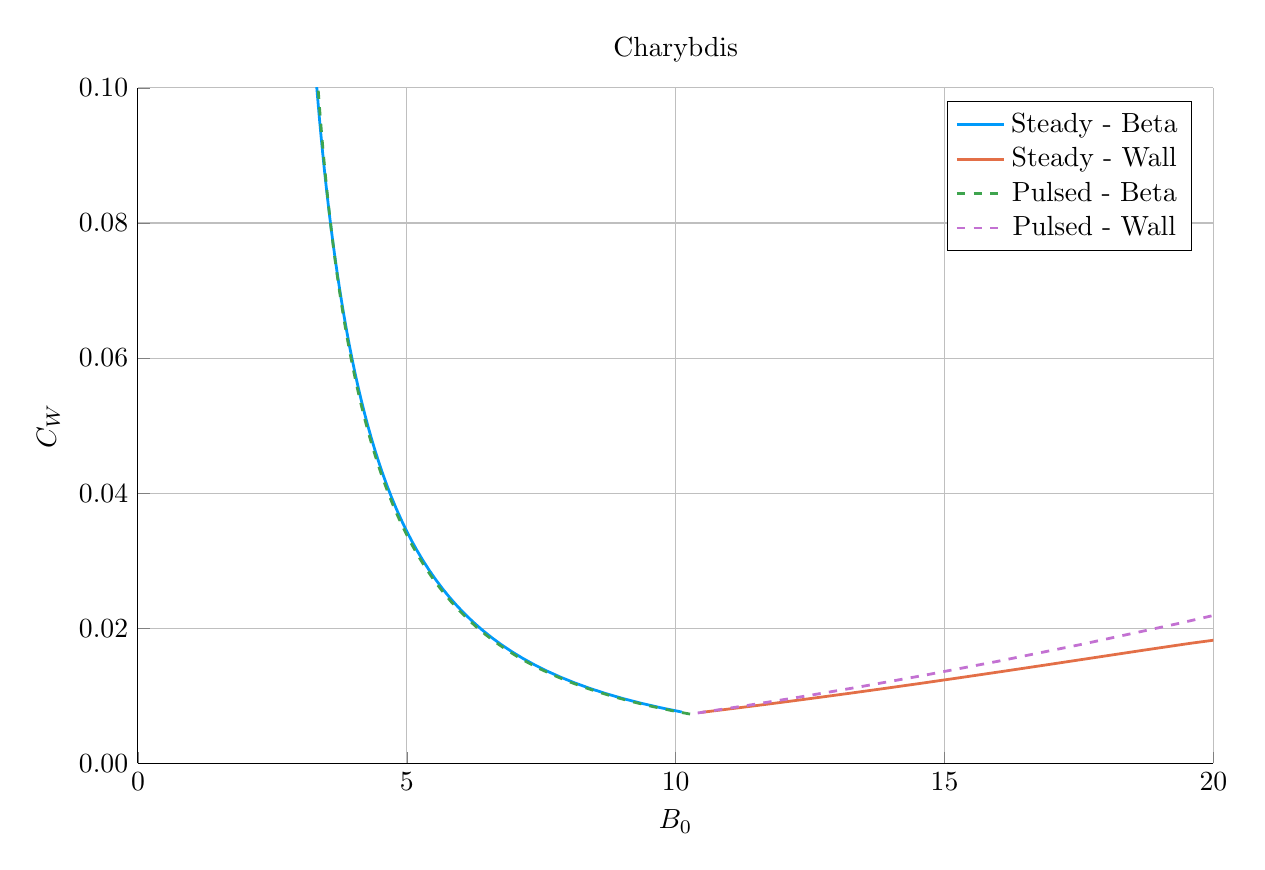
\begin{tikzpicture}[]
\begin{axis}[height = {101.6mm}, ylabel = {${C}_{W}$}, title = {Charybdis}, xmin = {0.0}, xmax = {20.0}, ymax = {0.1}, xlabel = {${B}_{0}$}, {unbounded coords=jump, scaled x ticks = false, xticklabel style={rotate = 0}, xmajorgrids = true, xtick = {0.0,5.0,10.0,15.0,20.0}, xticklabels = {0,5,10,15,20}, xtick align = inside, axis lines* = left, scaled y ticks = false, yticklabel style={rotate = 0}, ymajorgrids = true, ytick = {0.0,0.02,0.04,0.06,0.08,0.1}, yticklabels = {0.00,0.02,0.04,0.06,0.08,0.10}, ytick align = inside, axis lines* = left,     xshift = 0.0mm,
    yshift = 0.0mm,
    axis background/.style={fill={rgb,1:red,1.00000000;green,1.00000000;blue,1.00000000}}
, colorbar style={title=}}, ymin = {0.0}, width = {152.4mm}]\addplot+ [color = {rgb,1:red,0.00000000;green,0.60560316;blue,0.97868012},
draw opacity=1.0,
line width=1,
solid,mark = none,
mark size = 2.0,
mark options = {
    color = {rgb,1:red,0.00000000;green,0.00000000;blue,0.00000000}, draw opacity = 1.0,
    fill = {rgb,1:red,0.00000000;green,0.60560316;blue,0.97868012}, fill opacity = 1.0,
    line width = 1,
    rotate = 0,
    solid
}]coordinates {
(10.112818033153026, 0.007598383414978856)
(9.722156888543116, 0.008230424223188452)
(9.357875603858393, 0.008896404207575682)
(9.017653755630063, 0.009597023567402527)
(8.6995124437054, 0.010332804662622194)
(8.401566530516865, 0.011104394978990672)
(8.122163706328223, 0.011912345200844093)
(7.859819415455661, 0.012757161102175962)
(7.613196557650265, 0.013639302343912054)
(7.381088038653343, 0.014559181429827196)
(7.162401716104116, 0.015517162820285028)
(6.956147367527331, 0.016513562202290014)
(6.761425371986388, 0.017548645913683623)
(6.577416849463348, 0.018622630518712633)
(6.403375044688587, 0.019735682531644493)
(6.2386177769852695, 0.02088791828458706)
(6.0825208065966905, 0.022079403933712667)
(5.934511989185341, 0.02331015560822712)
(5.794066116682695, 0.024580139674436858)
(5.660700347012839, 0.02588927313954039)
(5.533970150598111, 0.027237424167073223)
(5.413465705416883, 0.02862441270831249)
(5.298808685607224, 0.03005001123436344)
(5.189649392059402, 0.031513945582432444)
(5.085664187259174, 0.033015895883282464)
(4.986553195072601, 0.03455549758379169)
(4.892038235455667, 0.03613234255000151)
(4.801860966679364, 0.037745980245626594)
(4.7157812114040425, 0.03939591897965519)
(4.633575445956479, 0.041081627216715676)
(4.5550354347559185, 0.04280253494397791)
(4.479966994069385, 0.04455803508845128)
(4.408188871204256, 0.046347484978679)
(4.33953172691477, 0.048170207844964834)
(4.273837210246432, 0.05002549435242988)
(4.210957116299974, 0.051912604161371986)
(4.15075261849161, 0.053830767509593334)
(4.0930935678432965, 0.05577918681155204)
(4.037857852672517, 0.05775703826940529)
(3.9849308127842145, 0.05976347349121981)
(3.9342047029103653, 0.06179762111185749)
(3.8855782007091695, 0.06385858841225403)
(3.838955955133626, 0.06594546293303978)
(3.7942481714200484, 0.06805731407868133)
(3.7513702293348077, 0.07019319470855978)
(3.710242331663442, 0.07235214271160313)
(3.6707891802306123, 0.0745331825613442)
(3.6329396770109583, 0.07673532684849063)
(3.5966266481325166, 0.07895757778829673)
(3.5617865887889004, 0.08119892870027327)
(3.5283594272686503, 0.08345836545794902)
(3.496288306480746, 0.08573486790664452)
(3.465519381509793, 0.08802741124736263)
(3.4360016318699595, 0.09033496738515884)
(3.4076866872513096, 0.0926565062404898)
(3.380528665662031, 0.09499099702224018)
(3.3544840229690007, 0.09733740946131986)
(3.3295114129297314, 0.09969471500383864)
(3.3055715568879336, 0.10206188796308927)
(3.2826271223788512, 0.10443790662966322)
(3.260642607548369, 0.10682175444066445)
(3.239584247604666, 0.10921242049746493)
(3.2194198921826622, 0.11160890156230109)
(3.2001189373344725, 0.11401020198268878)
(3.181652227422265, 0.11641533509457672)
(3.163991977015565, 0.11882332397376366)
(3.1471116955378684, 0.12123320224599504)
(3.130986116696265, 0.12364401485456963)
(3.115591132350856, 0.1260548187858383)
(3.1009037305081053, 0.12846468375306214)
(3.0869019371473265, 0.13087269283917113)
(3.0735647616124355, 0.13327794309901428)
(3.0608721453218655, 0.13567954612178545)
};
\addlegendentry{Steady - Beta}
\addplot+ [color = {rgb,1:red,0.88887350;green,0.43564919;blue,0.27812294},
draw opacity=1.0,
line width=1,
solid,mark = none,
mark size = 2.0,
mark options = {
    color = {rgb,1:red,0.00000000;green,0.00000000;blue,0.00000000}, draw opacity = 1.0,
    fill = {rgb,1:red,0.88887350;green,0.43564919;blue,0.27812294}, fill opacity = 1.0,
    line width = 1,
    rotate = 0,
    solid
}]coordinates {
(20.758867641064707, 0.018765308409143346)
(20.346250098246923, 0.018594952760163406)
(19.57104597888471, 0.01777146918538113)
(18.681781921115476, 0.016727851446155666)
(17.775790175980152, 0.015638576778075435)
(16.896654716492492, 0.014581653280825104)
(16.063927450323227, 0.013591211730165224)
(15.285557510665852, 0.012680275903338053)
(14.563500533069154, 0.01185123263968419)
(13.896568848875791, 0.01110114677254841)
(13.281970890030232, 0.010424581221258129)
(12.716170469467318, 0.009815118917575654)
(12.195372283741088, 0.00926617943914564)
(11.715794270833433, 0.008771443174384838)
(11.273815669498969, 0.008325054959037046)
(10.866051794088186, 0.007921704192505699)
(10.489365023931143, 0.007556609136513177)
};
\addlegendentry{Steady - Wall}
\addplot+ [color = {rgb,1:red,0.24222430;green,0.64327509;blue,0.30444865},
draw opacity=1.0,
line width=1,
dashed,mark = none,
mark size = 2.0,
mark options = {
    color = {rgb,1:red,0.00000000;green,0.00000000;blue,0.00000000}, draw opacity = 1.0,
    fill = {rgb,1:red,0.24222430;green,0.64327509;blue,0.30444865}, fill opacity = 1.0,
    line width = 1,
    rotate = 0,
    solid
}]coordinates {
(10.26788634689966, 0.007291637162809203)
(9.953967652326213, 0.007763018579561715)
(9.567926244368271, 0.008410560830066265)
(9.207974394987358, 0.009093056690349528)
(8.871841888699304, 0.009811202030777346)
(8.557505525932248, 0.010565644256199823)
(8.263156925406376, 0.01135697964954635)
(7.9871752024348766, 0.01218575089778548)
(7.728103682045175, 0.013052444820635726)
(7.484629973620137, 0.01395749030938975)
(7.255568856523303, 0.014901256485610468)
(7.039847526735421, 0.015884051087442074)
(6.836492834698909, 0.01690611908975986)
(6.644620209081183, 0.01796764156282338)
(6.463424013335149, 0.01906873477252413)
(6.2921691243175495, 0.020209449523749864)
(6.13018355681404, 0.02138977074682875)
(5.97685198655569, 0.022609617323612653)
(5.831610044919842, 0.023868842161338135)
(5.693939286027163, 0.025167232481888336)
(5.563362729090489, 0.026504510357656302)
(5.439440906144732, 0.0278803334592314)
(5.321768347746793, 0.02929429601917866)
(5.209970453003084, 0.030745929990983068)
(5.103700692769835, 0.03223470641747899)
(5.002638109938164, 0.03376003696406285)
(4.906485077678376, 0.03532127563010485)
(4.814965286571576, 0.03691772061565451)
(4.727821933804548, 0.03854861633202897)
(4.644816091323922, 0.04021315554278132)
(4.565725232806084, 0.04191048162126061)
(4.490341901840154, 0.04363969091085349)
(4.418472505906755, 0.04539983517396531)
(4.349936222622964, 0.047189924115870814)
(4.284564006352339, 0.049008927969770806)
(4.222197684694192, 0.05085578012965056)
(4.162689135592264, 0.05272937981792158)
(4.105899536872315, 0.05462859477526984)
(4.051698680949713, 0.056552263960658246)
(3.9999643482627323, 0.058499200250012214)
(3.9505817337017928, 0.06046819312273483)
(3.903442920928527, 0.062458011325916454)
(3.858446400032002, 0.06446740550676137)
(3.8154966244515616, 0.06649511080452623)
(3.7745036035252744, 0.06853984939399767)
(3.7353825273991994, 0.07060033297331114)
(3.6980534213689746, 0.07267526518964869)
(3.6624408270205375, 0.07476334399712868)
(3.62847350780097, 0.07686326394192533)
(3.5960841768845415, 0.07897371837037194)
(3.565209245407392, 0.08109340155652811)
(3.5357885893311605, 0.0832210107463015)
(3.5077653333614305, 0.08535524811591486)
(3.4810856504959875, 0.08749482264305544)
(3.4556985759109375, 0.08963845188964095)
(3.4315558340122845, 0.09178486369563649)
(3.408611677587535, 0.09393279778385825)
(3.3868227380888998, 0.09608100727612065)
(3.36614788616562, 0.09822826012150637)
(3.3465481016421226, 0.10037334043786662)
(3.327986352208224, 0.1025150497680155)
(3.3104274769652595, 0.10465220838353721)
(3.2938380965241474, 0.1067836557197021)
(3.278186482171801, 0.10890825269906537)
(3.263442495132517, 0.11102488135374605)
(3.2495774839156075, 0.1131324463411963)
(3.236564206241785, 0.11522987560063444)
(3.224376752844934, 0.11731612107126856)
(3.212990475972638, 0.11939015934381376)
(3.2023819222517877, 0.12145099224802183)
(3.192528769611062, 0.12349764737898258)
(3.1834097679780142, 0.1255291785649034)
(3.1750046834890777, 0.12754466627907632)
(3.1672942459724482, 0.12954321799866983)
};
\addlegendentry{Pulsed - Beta}
\addplot+ [color = {rgb,1:red,0.76444018;green,0.44411178;blue,0.82429754},
draw opacity=1.0,
line width=1,
dashed,mark = none,
mark size = 2.0,
mark options = {
    color = {rgb,1:red,0.00000000;green,0.00000000;blue,0.00000000}, draw opacity = 1.0,
    fill = {rgb,1:red,0.76444018;green,0.44411178;blue,0.82429754}, fill opacity = 1.0,
    line width = 1,
    rotate = 0,
    solid
}]coordinates {
(48.990476413653056, 0.09724163307501366)
(42.83950920694117, 0.07766994779263652)
(37.687790427214495, 0.06269593244609177)
(33.33937742845888, 0.05109841711622891)
(29.64296398154308, 0.04201539110057761)
(26.48039367255613, 0.034828857187910324)
(23.758442882319894, 0.029089432591006322)
(21.402860298405816, 0.02446606951047545)
(19.353987387634486, 0.020711961258999954)
(17.563502020363714, 0.017641064746807725)
(15.991970371213752, 0.015111701839397276)
(14.606987499719377, 0.013014953187280779)
(13.381751501116137, 0.011266342778060628)
(12.293960329570087, 0.009799811915435606)
(11.32495111804522, 0.00856330563618739)
(10.459023415380802, 0.007515507834648486)
(10.26788634689966, 0.007291637162809203)
};
\addlegendentry{Pulsed - Wall}
\end{axis}

\end{tikzpicture}

		\end{adjustbox}
        \caption{Charybdis}
    \end{subfigure}
    \hfill
    \begin{subfigure}[t]{0.45\textwidth}
        \centering
		\begin{adjustbox}{width=\textwidth}
			\Large
			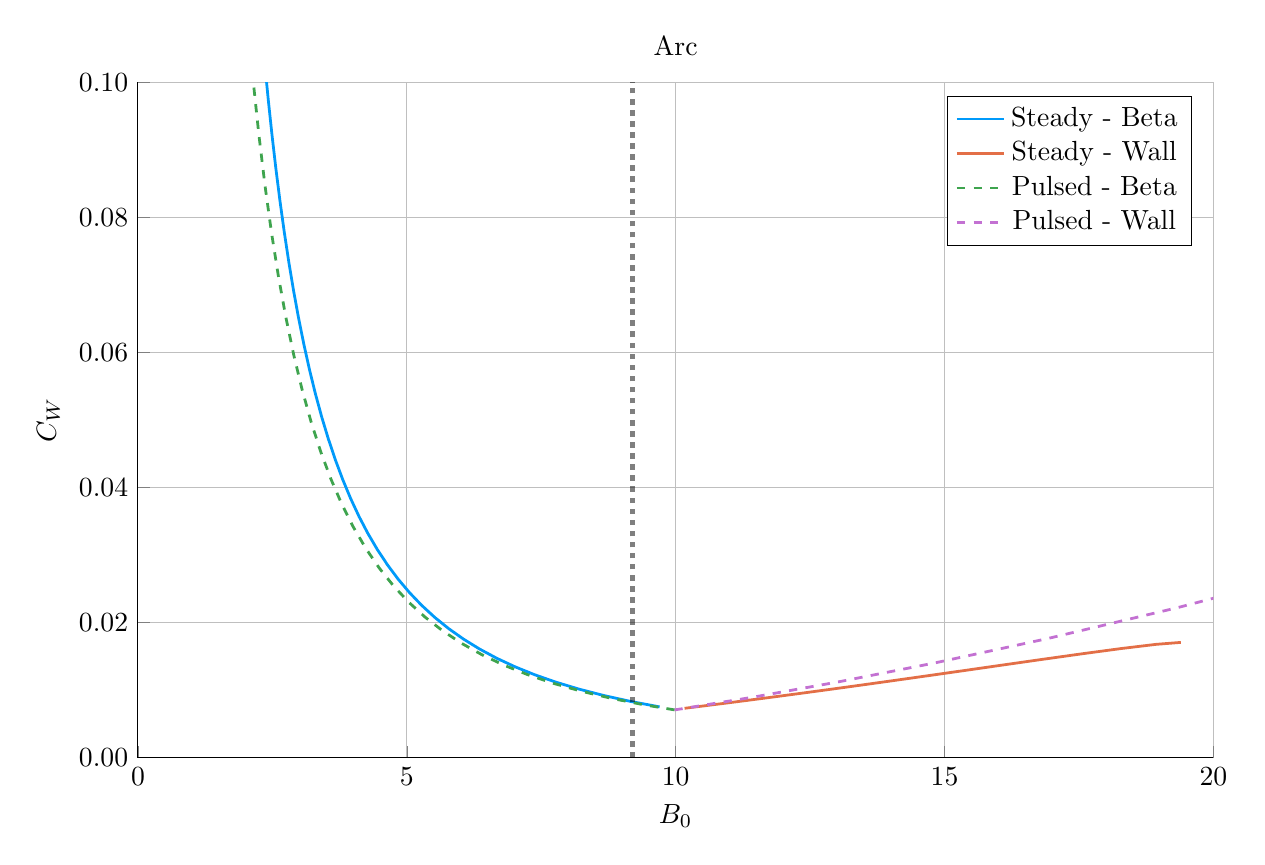
\begin{tikzpicture}[]
\begin{axis}[height = {101.6mm}, ylabel = {${C}_{W}$}, title = {Arc}, xmin = {0.0}, xmax = {20.0}, ymax = {0.1}, xlabel = {${B}_{0}$}, {unbounded coords=jump, scaled x ticks = false, xticklabel style={rotate = 0}, xmajorgrids = true, xtick = {0.0,5.0,10.0,15.0,20.0}, xticklabels = {0,5,10,15,20}, xtick align = inside, axis lines* = left, scaled y ticks = false, yticklabel style={rotate = 0}, ymajorgrids = true, ytick = {0.0,0.02,0.04,0.06,0.08,0.1}, yticklabels = {0.00,0.02,0.04,0.06,0.08,0.10}, ytick align = inside, axis lines* = left,     xshift = 0.0mm,
    yshift = 0.0mm,
    axis background/.style={fill={rgb,1:red,1.00000000;green,1.00000000;blue,1.00000000}}
, colorbar style={title=}}, ymin = {0.0}, width = {152.4mm}]\addplot+ [color = {rgb,1:red,0.00000000;green,0.60560316;blue,0.97868012},
draw opacity=1.0,
line width=1,
solid,mark = none,
mark size = 2.0,
mark options = {
    color = {rgb,1:red,0.00000000;green,0.00000000;blue,0.00000000}, draw opacity = 1.0,
    fill = {rgb,1:red,0.00000000;green,0.60560316;blue,0.97868012}, fill opacity = 1.0,
    line width = 1,
    rotate = 0,
    solid
}]coordinates {
(9.701206080853105, 0.00751651377736839)
(9.162315904693079, 0.008323905812934898)
(8.664301107137337, 0.009198905086222158)
(8.203576462497304, 0.010145151644824739)
(7.776718537485166, 0.011166668317960562)
(7.380720231870917, 0.012267478183796882)
(7.012886014999712, 0.013451673110529961)
(6.670795005901889, 0.014723405583659413)
(6.352268997292712, 0.01608688012694734)
(6.055344682097163, 0.017546344352390175)
(5.778249464564785, 0.019106079676451882)
(5.519380338856715, 0.020770391741442663)
(5.2772854007125325, 0.02254360058225732)
(5.050647625972996, 0.02443003057971548)
(4.838270606140816, 0.026434000242494555)
(4.639065978019038, 0.028559811860080504)
(4.4520423235376105, 0.030811741069328453)
(4.276295348572609, 0.03319402637711819)
(4.110999177018484, 0.03571085868120887)
(3.9553986195015125, 0.038366370830779505)
(3.8088022956698633, 0.041164627267286334)
(3.6705765055641186, 0.04410961378519341)
(3.54013975965751, 0.047205227450858)
(3.4169578891619192, 0.050455266716399376)
(3.30053966845824, 0.05386342176374704)
(3.1904328903033052, 0.05743326511231589)
(3.086220842019516, 0.061168242521834885)
(2.9875191373772063, 0.0650716642198721)
(2.8939728644914635, 0.0691466964814904)
(2.8052540149097247, 0.07339635358630757)
(2.7210591632720242, 0.07782349017600093)
(2.6411073705789065, 0.08243079403304142)
(2.565138287279709, 0.08722077929915266)
(2.492910435164382, 0.09219578014969385)
(2.4241996494611984, 0.09735794493788336)
(2.3587976646588236, 0.10270923082049731)
(2.296510829425685, 0.10825139887447487)
(2.237158937627476, 0.11398600971161459)
(2.180574163874242, 0.11991441959647205)
(2.126600093288366, 0.1260377770704313)
(2.075090836295778, 0.1323570200829707)
(2.0259102202234582, 0.13887287362917833)
(1.978931050353818, 0.14558584789074455)
(1.9340344338545452, 0.15249623687593467)
(1.8911091606836798, 0.1596041175523241)
(1.8500511361739687, 0.16690934946459546)
(1.8107628605384507, 0.17441157482817518)
(1.773152951016952, 0.1821102190881948)
(1.7371357028100902, 0.19000449193192903)
(1.7026306853269466, 0.19809338874181076)
(1.6695623706125668, 0.2063756924750063)
(1.6378597911249178, 0.21484997595463062)
(1.607456224302725, 0.22351460455684893)
(1.5782889016090462, 0.23236773927733403)
(1.5502987399539199, 0.24140734015998855)
(1.5234300935954943, 0.2506311700702061)
(1.4976305247952577, 0.26003679879456143)
(1.4728505916614916, 0.26962160744844355)
(1.4490436517578602, 0.2793827931728701)
(1.4261656801829077, 0.2893173741014787)
};
\addlegendentry{Steady - Beta}
\addplot+ [color = {rgb,1:red,0.88887350;green,0.43564919;blue,0.27812294},
draw opacity=1.0,
line width=1,
solid,mark = none,
mark size = 2.0,
mark options = {
    color = {rgb,1:red,0.00000000;green,0.00000000;blue,0.00000000}, draw opacity = 1.0,
    fill = {rgb,1:red,0.88887350;green,0.43564919;blue,0.27812294}, fill opacity = 1.0,
    line width = 1,
    rotate = 0,
    solid
}]coordinates {
(19.394007482712425, 0.017062717610395756)
(18.932196567189358, 0.01677318247708789)
(18.296989378345195, 0.01616608087020061)
(17.587029315408756, 0.015409201334794807)
(16.847882407994106, 0.014583614099307054)
(16.111374502564406, 0.01374625755936427)
(15.396027314547156, 0.012930331454144767)
(14.710952688793137, 0.012152313568351602)
(14.06168447794857, 0.011421914699879928)
(13.450465418483889, 0.010742972750322424)
(12.877644538645335, 0.010115989865118968)
(12.342394470642008, 0.009539468548127306)
(11.843182246608265, 0.00901077532361949)
(11.376441269625893, 0.008524384373336923)
(10.944966372727551, 0.008083786116178366)
(10.541663878705513, 0.007678592362816001)
(10.165908182236457, 0.0073076305932358344)
};
\addlegendentry{Steady - Wall}
\addplot+ [color = {rgb,1:red,0.24222430;green,0.64327509;blue,0.30444865},
draw opacity=1.0,
line width=1,
dashed,mark = none,
mark size = 2.0,
mark options = {
    color = {rgb,1:red,0.00000000;green,0.00000000;blue,0.00000000}, draw opacity = 1.0,
    fill = {rgb,1:red,0.24222430;green,0.64327509;blue,0.30444865}, fill opacity = 1.0,
    line width = 1,
    rotate = 0,
    solid
}]coordinates {
(9.980483622051658, 0.007070839678110688)
(9.392786903460065, 0.007852618677281367)
(8.79273598103983, 0.008801125480455354)
(8.23820290909994, 0.009848957316818736)
(7.725182218401588, 0.011005021009379608)
(7.250078106370205, 0.012278877224830715)
(6.80965553466646, 0.013680774995781924)
(6.400998063035608, 0.01522168706241675)
(6.0214713600430425, 0.01691334607316053)
(5.668691517461799, 0.01876828173242221)
(5.340497445229901, 0.020799859050557753)
(5.034926745580058, 0.02302231794191222)
(4.750194564008521, 0.02545081453735327)
(4.484674995755211, 0.028101464735781394)
(4.236884692979903, 0.030991390724248)
(4.00546837264544, 0.03413877146046793)
(3.7891859704718387, 0.03756289844971818)
(3.5869012239550364, 0.04128423857957625)
(3.3975714987448393, 0.04532450632539042)
(3.2202386987489797, 0.04970674833925621)
(3.0540211220494466, 0.05445544432876858)
(2.8981061427709687, 0.059596629277403584)
(2.7517436139566023, 0.06515804353669719)
(2.6142398986781377, 0.07116931924441194)
(2.4849524463010138, 0.07766221405391976)
(2.363284838174807, 0.08467090653190464)
(2.248682232019848, 0.09223237213933476)
(2.140627136740878, 0.10038686497222395)
(2.038635448877246, 0.10917853919500715)
(1.9422526775794744, 0.11865625658225108)
(1.8510502754751532, 0.12887464475233826)
(1.7646219756564088, 0.1398954977169483)
(1.6825800061969869, 0.15178965160557917)
(1.6045510059627948, 0.16463953300974782)
(1.53017138625397, 0.17854268160508957)
(1.4590817483192686, 0.19361672262027943)
(1.3909197311384796, 0.21000656636649426)
(1.3253102336217724, 0.22789515931839086)
(1.261851128383913, 0.24752015854836598)
(1.20009089049112, 0.2692010388315911)
(1.1394908096975784, 0.2933858656724498)
};
\addlegendentry{Pulsed - Beta}
\addplot+ [color = {rgb,1:red,0.76444018;green,0.44411178;blue,0.82429754},
draw opacity=1.0,
line width=1,
dashed,mark = none,
mark size = 2.0,
mark options = {
    color = {rgb,1:red,0.00000000;green,0.00000000;blue,0.00000000}, draw opacity = 1.0,
    fill = {rgb,1:red,0.76444018;green,0.44411178;blue,0.82429754}, fill opacity = 1.0,
    line width = 1,
    rotate = 0,
    solid
}]coordinates {
(29.27715761652869, 0.045433420664911836)
(25.4410619834368, 0.0356668159806907)
(22.158819835998365, 0.02810552804100701)
(19.342453256965573, 0.02222656993153558)
(16.919364280634177, 0.0176372518175528)
(14.829378672669455, 0.014041066675248008)
(13.022412368922526, 0.011212962182114766)
(11.456617692058645, 0.00898128637894181)
(10.096901921254785, 0.00721451699843558)
(9.980483622051658, 0.007070839678110688)
};
\addlegendentry{Pulsed - Wall}
\addplot+ [color = {rgb,1:red,0.00000000;green,0.00000000;blue,0.00000000},
draw opacity=0.5,
line width=2,
dotted,mark = none,
mark size = 2.0,
mark options = {
    color = {rgb,1:red,0.00000000;green,0.00000000;blue,0.00000000}, draw opacity = 0.5,
    fill = {rgb,1:red,0.00000000;green,0.00000000;blue,0.00000000}, fill opacity = 0.5,
    line width = 1,
    rotate = 0,
    solid
},forget plot]coordinates {
(0.0, NaN)
(20.0, NaN)
};
\addplot+ [color = {rgb,1:red,0.00000000;green,0.00000000;blue,0.00000000},
draw opacity=0.5,
line width=2,
dotted,mark = none,
mark size = 2.0,
mark options = {
    color = {rgb,1:red,0.00000000;green,0.00000000;blue,0.00000000}, draw opacity = 0.5,
    fill = {rgb,1:red,0.00000000;green,0.00000000;blue,0.00000000}, fill opacity = 0.5,
    line width = 1,
    rotate = 0,
    solid
},forget plot]coordinates {
(9.2, 0.0)
(9.2, 0.1)
};
\addplot+[draw=none, color = {rgb,1:red,0.00000000;green,0.00000000;blue,0.00000000},
draw opacity=0.5,
line width=0,
solid,mark = *,
mark size = 2.0,
mark options = {
    color = {rgb,1:red,0.00000000;green,0.00000000;blue,0.00000000}, draw opacity = 0.5,
    fill = {rgb,1:red,0.00000000;green,0.00000000;blue,0.00000000}, fill opacity = 0.5,
    line width = 1,
    rotate = 0,
    solid
},forget plot] coordinates {
(9.2, NaN)
};
\end{axis}

\end{tikzpicture}

		\end{adjustbox}
        \caption{Arc}
    \end{subfigure}
    \hfill \hfill ~\\ ~\\ ~\\ ~\\
    \hfill 
    \begin{subfigure}[t]{0.45\textwidth}
        \centering
		\begin{adjustbox}{width=\textwidth}
			\Large
			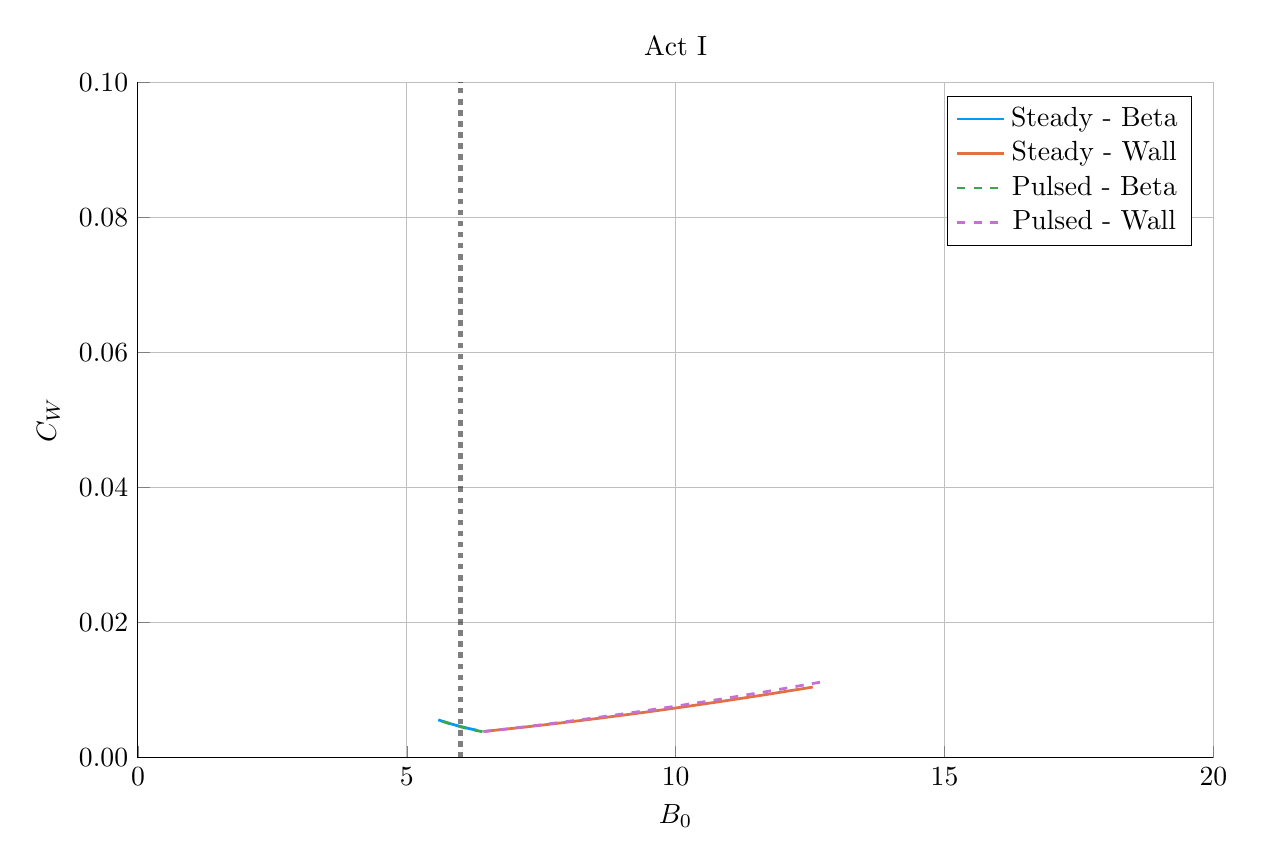
\begin{tikzpicture}[]
\begin{axis}[height = {101.6mm}, ylabel = {${C}_{W}$}, title = {Act I}, xmin = {0.0}, xmax = {20.0}, ymax = {0.1}, xlabel = {${B}_{0}$}, {unbounded coords=jump, scaled x ticks = false, xticklabel style={rotate = 0}, xmajorgrids = true, xtick = {0.0,5.0,10.0,15.0,20.0}, xticklabels = {0,5,10,15,20}, xtick align = inside, axis lines* = left, scaled y ticks = false, yticklabel style={rotate = 0}, ymajorgrids = true, ytick = {0.0,0.02,0.04,0.06,0.08,0.1}, yticklabels = {0.00,0.02,0.04,0.06,0.08,0.10}, ytick align = inside, axis lines* = left,     xshift = 0.0mm,
    yshift = 0.0mm,
    axis background/.style={fill={rgb,1:red,1.00000000;green,1.00000000;blue,1.00000000}}
, colorbar style={title=}}, ymin = {0.0}, width = {152.4mm}]\addplot+ [color = {rgb,1:red,0.00000000;green,0.60560316;blue,0.97868012},
draw opacity=1.0,
line width=1,
solid,mark = none,
mark size = 2.0,
mark options = {
    color = {rgb,1:red,0.00000000;green,0.00000000;blue,0.00000000}, draw opacity = 1.0,
    fill = {rgb,1:red,0.00000000;green,0.60560316;blue,0.97868012}, fill opacity = 1.0,
    line width = 1,
    rotate = 0,
    solid
}]coordinates {
(6.30336807958207, 0.004055552148042579)
(6.162193069273141, 0.004300298316165893)
(6.030717178404645, 0.004550498291731095)
(5.908065509576601, 0.004805976791051415)
(5.793464904530972, 0.005066558265934883)
(5.686229631357383, 0.005332067188485748)
(5.585749511271037, 0.005602328191394613)
};
\addlegendentry{Steady - Beta}
\addplot+ [color = {rgb,1:red,0.88887350;green,0.43564919;blue,0.27812294},
draw opacity=1.0,
line width=1,
solid,mark = none,
mark size = 2.0,
mark options = {
    color = {rgb,1:red,0.00000000;green,0.00000000;blue,0.00000000}, draw opacity = 1.0,
    fill = {rgb,1:red,0.88887350;green,0.43564919;blue,0.27812294}, fill opacity = 1.0,
    line width = 1,
    rotate = 0,
    solid
}]coordinates {
(12.549536249695134, 0.010450364750783054)
(11.658754653696462, 0.009311160177277214)
(10.883719833507003, 0.008367979762533702)
(10.206258129789394, 0.007581000508027489)
(9.611335769312953, 0.0069194030019139735)
(9.086446934250878, 0.006359119854353646)
(8.62129895070743, 0.0058814059200114925)
(8.207216040989662, 0.005471332591600982)
(7.837119555085499, 0.005117248050094358)
(7.505047858717157, 0.00480979217186778)
(7.20604322925957, 0.0045414928704811935)
(6.935884710193303, 0.0043062495703983395)
(6.691016583192173, 0.004099109819554263)
(6.468415485086983, 0.0039160098791423655)
};
\addlegendentry{Steady - Wall}
\addplot+ [color = {rgb,1:red,0.24222430;green,0.64327509;blue,0.30444865},
draw opacity=1.0,
line width=1,
dashed,mark = none,
mark size = 2.0,
mark options = {
    color = {rgb,1:red,0.00000000;green,0.00000000;blue,0.00000000}, draw opacity = 1.0,
    fill = {rgb,1:red,0.24222430;green,0.64327509;blue,0.30444865}, fill opacity = 1.0,
    line width = 1,
    rotate = 0,
    solid
}]coordinates {
(6.408263337806559, 0.003837054084878144)
(6.408263337806564, 0.0038370540848781357)
(6.385466513301022, 0.003872993818821736)
(6.245492502072912, 0.004106512578517519)
(6.116010320461132, 0.004344317387601225)
(5.9960421481916395, 0.004586160922256416)
(5.884727159112828, 0.004831799090393476)
(5.781304768121868, 0.00508099132781059)
(5.685100648450046, 0.005333500860613775)
(5.595515000321003, 0.005589094940610307)
};
\addlegendentry{Pulsed - Beta}
\addplot+ [color = {rgb,1:red,0.76444018;green,0.44411178;blue,0.82429754},
draw opacity=1.0,
line width=1,
dashed,mark = none,
mark size = 2.0,
mark options = {
    color = {rgb,1:red,0.00000000;green,0.00000000;blue,0.00000000}, draw opacity = 1.0,
    fill = {rgb,1:red,0.76444018;green,0.44411178;blue,0.82429754}, fill opacity = 1.0,
    line width = 1,
    rotate = 0,
    solid
}]coordinates {
(12.684248532650473, 0.011163257244949718)
(11.66307871570063, 0.009745831059904)
(10.781888309639141, 0.008590800927445573)
(10.016282491385791, 0.007639361749178777)
(9.346943280276514, 0.006847895899781745)
(8.758420158941194, 0.0061835958355957316)
(8.238241792953433, 0.005621466066992172)
(7.776255600865612, 0.005142236201168238)
(7.364131118520045, 0.0047308861724008975)
(6.994982564641668, 0.00437558945422717)
(6.66307916140573, 0.004066945929726434)
(6.408263337806559, 0.003837054084878144)
(6.408263337806564, 0.0038370540848781357)
};
\addlegendentry{Pulsed - Wall}
\addplot+ [color = {rgb,1:red,0.00000000;green,0.00000000;blue,0.00000000},
draw opacity=0.5,
line width=2,
dotted,mark = none,
mark size = 2.0,
mark options = {
    color = {rgb,1:red,0.00000000;green,0.00000000;blue,0.00000000}, draw opacity = 0.5,
    fill = {rgb,1:red,0.00000000;green,0.00000000;blue,0.00000000}, fill opacity = 0.5,
    line width = 1,
    rotate = 0,
    solid
},forget plot]coordinates {
(0.0, NaN)
(20.0, NaN)
};
\addplot+ [color = {rgb,1:red,0.00000000;green,0.00000000;blue,0.00000000},
draw opacity=0.5,
line width=2,
dotted,mark = none,
mark size = 2.0,
mark options = {
    color = {rgb,1:red,0.00000000;green,0.00000000;blue,0.00000000}, draw opacity = 0.5,
    fill = {rgb,1:red,0.00000000;green,0.00000000;blue,0.00000000}, fill opacity = 0.5,
    line width = 1,
    rotate = 0,
    solid
},forget plot]coordinates {
(6.0, 0.0)
(6.0, 0.1)
};
\addplot+[draw=none, color = {rgb,1:red,0.00000000;green,0.00000000;blue,0.00000000},
draw opacity=0.5,
line width=0,
solid,mark = *,
mark size = 2.0,
mark options = {
    color = {rgb,1:red,0.00000000;green,0.00000000;blue,0.00000000}, draw opacity = 0.5,
    fill = {rgb,1:red,0.00000000;green,0.00000000;blue,0.00000000}, fill opacity = 0.5,
    line width = 1,
    rotate = 0,
    solid
},forget plot] coordinates {
(6.0, NaN)
};
\end{axis}

\end{tikzpicture}

		\end{adjustbox}
        \caption{Act I}
    \end{subfigure}
    \hfill
    \begin{subfigure}[t]{0.45\textwidth}
        \centering
		\begin{adjustbox}{width=\textwidth}
			\Large
			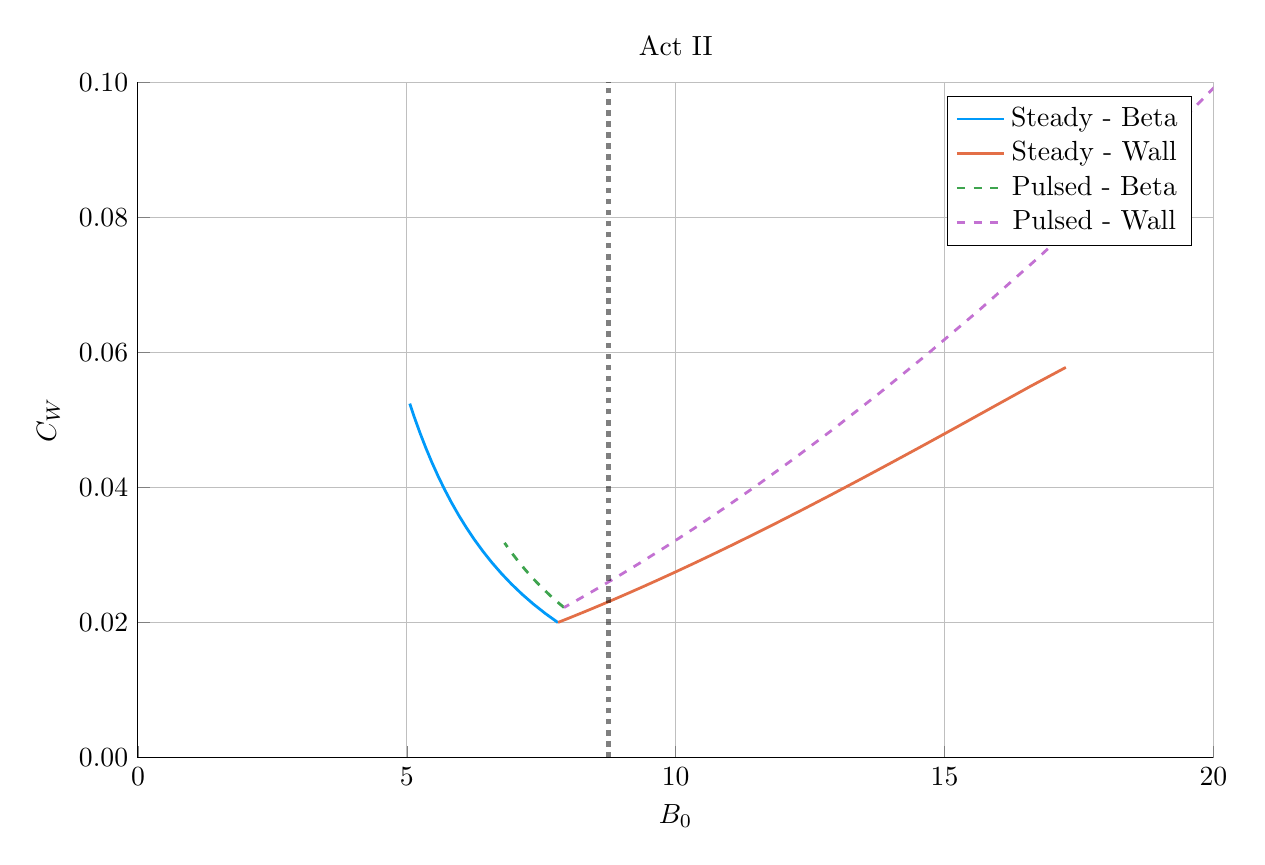
\begin{tikzpicture}[]
\begin{axis}[height = {101.6mm}, ylabel = {${C}_{W}$}, title = {Act II}, xmin = {0.0}, xmax = {20.0}, ymax = {0.1}, xlabel = {${B}_{0}$}, {unbounded coords=jump, scaled x ticks = false, xticklabel style={rotate = 0}, xmajorgrids = true, xtick = {0.0,5.0,10.0,15.0,20.0}, xticklabels = {0,5,10,15,20}, xtick align = inside, axis lines* = left, scaled y ticks = false, yticklabel style={rotate = 0}, ymajorgrids = true, ytick = {0.0,0.02,0.04,0.06,0.08,0.1}, yticklabels = {0.00,0.02,0.04,0.06,0.08,0.10}, ytick align = inside, axis lines* = left,     xshift = 0.0mm,
    yshift = 0.0mm,
    axis background/.style={fill={rgb,1:red,1.00000000;green,1.00000000;blue,1.00000000}}
, colorbar style={title=}}, ymin = {0.0}, width = {152.4mm}]\addplot+ [color = {rgb,1:red,0.00000000;green,0.60560316;blue,0.97868012},
draw opacity=1.0,
line width=1,
solid,mark = none,
mark size = 2.0,
mark options = {
    color = {rgb,1:red,0.00000000;green,0.00000000;blue,0.00000000}, draw opacity = 1.0,
    fill = {rgb,1:red,0.00000000;green,0.60560316;blue,0.97868012}, fill opacity = 1.0,
    line width = 1,
    rotate = 0,
    solid
}]coordinates {
(7.810935944285959, 0.019999870342781445)
(7.57736049850867, 0.02133467083845229)
(7.354864292609041, 0.022732819748494743)
(7.145167234136329, 0.024185030975062572)
(6.9473303865083675, 0.025691491983248542)
(6.760499508614096, 0.027252320661142464)
(6.583897990324067, 0.028867554534578326)
(6.416817229618043, 0.030537157829042417)
(6.258609820663305, 0.032261020375438675)
(6.108683264880386, 0.034038958296321455)
(5.966494431410919, 0.03587071487617403)
(5.831544666176381, 0.0377559616009066)
(5.703375459679132, 0.03969429938840844)
(5.581564609582325, 0.04168525992229865)
(5.465722802994068, 0.04372830718110872)
(5.355490573482678, 0.04582283908419109)
(5.25053558682053, 0.047968189231402746)
(5.1505502068221745, 0.0501636288266544)
(5.0552493196883175, 0.0524083686363995)
};
\addlegendentry{Steady - Beta}
\addplot+ [color = {rgb,1:red,0.88887350;green,0.43564919;blue,0.27812294},
draw opacity=1.0,
line width=1,
solid,mark = none,
mark size = 2.0,
mark options = {
    color = {rgb,1:red,0.00000000;green,0.00000000;blue,0.00000000}, draw opacity = 1.0,
    fill = {rgb,1:red,0.88887350;green,0.43564919;blue,0.27812294}, fill opacity = 1.0,
    line width = 1,
    rotate = 0,
    solid
}]coordinates {
(17.25550839059296, 0.057778872694714996)
(16.594334962335296, 0.05496298917461432)
(15.9071755430688, 0.05194082278283737)
(15.233983138507648, 0.04897170009560995)
(14.594239858921854, 0.04617848140750687)
(13.989673082630297, 0.04357183498888427)
(13.414782495717416, 0.041119354314331134)
(12.872659546281994, 0.03883879592226187)
(12.364365715508608, 0.03673485145929315)
(11.889507953196574, 0.03480335845855904)
(11.44685939646348, 0.0330353994524836)
(11.034739998180656, 0.03141974653036777)
(10.651252523287319, 0.02994431754557875)
(10.294428800132035, 0.02859703023052943)
(9.962319203963213, 0.02736628585076568)
(9.653045819449929, 0.0262412244397216)
(9.364832254395445, 0.02521184000785315)
(9.096018465506306, 0.02426901119368965)
(8.844373144802077, 0.023401030424376988)
(8.61055754360846, 0.022610816631964757)
(8.391192178573277, 0.021881336042883122)
(8.18577947665566, 0.021210054866812295)
(7.99323348423048, 0.020591621521449808)
(7.812301489248497, 0.02001998340874561)
};
\addlegendentry{Steady - Wall}
\addplot+ [color = {rgb,1:red,0.24222430;green,0.64327509;blue,0.30444865},
draw opacity=1.0,
line width=1,
dashed,mark = none,
mark size = 2.0,
mark options = {
    color = {rgb,1:red,0.00000000;green,0.00000000;blue,0.00000000}, draw opacity = 1.0,
    fill = {rgb,1:red,0.24222430;green,0.64327509;blue,0.30444865}, fill opacity = 1.0,
    line width = 1,
    rotate = 0,
    solid
}]coordinates {
(7.923668284887995, 0.02222721640664124)
(7.923668284887995, 0.022227216406641305)
(7.836759696043437, 0.022801804106215327)
(7.6662731560983355, 0.023999703560063156)
(7.50499428233835, 0.025227714472706875)
(7.35232773269976, 0.026485173676255868)
(7.207727224738343, 0.02777136956552452)
(7.070690693175276, 0.029085544281911353)
(6.940756001029682, 0.03042689602188544)
(6.817497143644154, 0.0317945813900804)
};
\addlegendentry{Pulsed - Beta}
\addplot+ [color = {rgb,1:red,0.76444018;green,0.44411178;blue,0.82429754},
draw opacity=1.0,
line width=1,
dashed,mark = none,
mark size = 2.0,
mark options = {
    color = {rgb,1:red,0.00000000;green,0.00000000;blue,0.00000000}, draw opacity = 1.0,
    fill = {rgb,1:red,0.76444018;green,0.44411178;blue,0.82429754}, fill opacity = 1.0,
    line width = 1,
    rotate = 0,
    solid
}]coordinates {
(22.56106430311702, 0.12077728813238993)
(20.85607192394036, 0.10611249618735387)
(19.335265246056654, 0.09369703436900484)
(17.974121547130903, 0.08312792497015177)
(16.751976718553127, 0.07408393734926945)
(15.651329744019142, 0.06630720048423838)
(14.65728744097675, 0.05958933132558854)
(13.757118584462601, 0.05376088392733976)
(12.939893642194303, 0.04868326015323384)
(12.196191964860315, 0.04424246074454113)
(11.517862472405039, 0.04034422355142677)
(10.897827027335556, 0.0369102154096456)
(10.329918077124672, 0.0338750302375444)
(9.808743940706389, 0.031183808185534914)
(9.329576544487265, 0.02879033654896873)
(8.888257451278507, 0.026655526551708646)
(8.481118883411932, 0.024746185235479588)
(8.10491708701527, 0.02303402032897385)
(7.923668284887995, 0.02222721640664124)
(7.923668284887995, 0.022227216406641305)
};
\addlegendentry{Pulsed - Wall}
\addplot+ [color = {rgb,1:red,0.00000000;green,0.00000000;blue,0.00000000},
draw opacity=0.5,
line width=2,
dotted,mark = none,
mark size = 2.0,
mark options = {
    color = {rgb,1:red,0.00000000;green,0.00000000;blue,0.00000000}, draw opacity = 0.5,
    fill = {rgb,1:red,0.00000000;green,0.00000000;blue,0.00000000}, fill opacity = 0.5,
    line width = 1,
    rotate = 0,
    solid
},forget plot]coordinates {
(0.0, NaN)
(20.0, NaN)
};
\addplot+ [color = {rgb,1:red,0.00000000;green,0.00000000;blue,0.00000000},
draw opacity=0.5,
line width=2,
dotted,mark = none,
mark size = 2.0,
mark options = {
    color = {rgb,1:red,0.00000000;green,0.00000000;blue,0.00000000}, draw opacity = 0.5,
    fill = {rgb,1:red,0.00000000;green,0.00000000;blue,0.00000000}, fill opacity = 0.5,
    line width = 1,
    rotate = 0,
    solid
},forget plot]coordinates {
(8.75, 0.0)
(8.75, 0.1)
};
\addplot+[draw=none, color = {rgb,1:red,0.00000000;green,0.00000000;blue,0.00000000},
draw opacity=0.5,
line width=0,
solid,mark = *,
mark size = 2.0,
mark options = {
    color = {rgb,1:red,0.00000000;green,0.00000000;blue,0.00000000}, draw opacity = 0.5,
    fill = {rgb,1:red,0.00000000;green,0.00000000;blue,0.00000000}, fill opacity = 0.5,
    line width = 1,
    rotate = 0,
    solid
},forget plot] coordinates {
(8.75, NaN)
};
\end{axis}

\end{tikzpicture}

		\end{adjustbox}
        \caption{Act II}
    \end{subfigure}
    \hfill \hfill ~\\ ~\\ ~\\
    \caption{Steady State Cost Curves}
    \label{fig:steady_cost}
\end{figure*}

The problem of selecting an optimum design is more difficult for the pulsed case. This is mainly due to the kink limit regime being actually achievable. Following the conclusion from steady-state reactors would be an oversimplification because there are actually two costs relevant to reactors: capital cost and cost-per-watt. These beta-wall reactors are actually the points often best for minimizing cost-per-watt (i.e. your rate of return). The new beta-kink reactors, then, lead to cheap to build machines -- ones with a minimum capital cost. These conclusions are shown in \cref{fig:pulsed_costs}.

\begin{figure*}
    \centering
    \hfill 
    \begin{subfigure}[t]{0.45\textwidth}
        \centering
		\begin{adjustbox}{width=\textwidth}
			\Large
			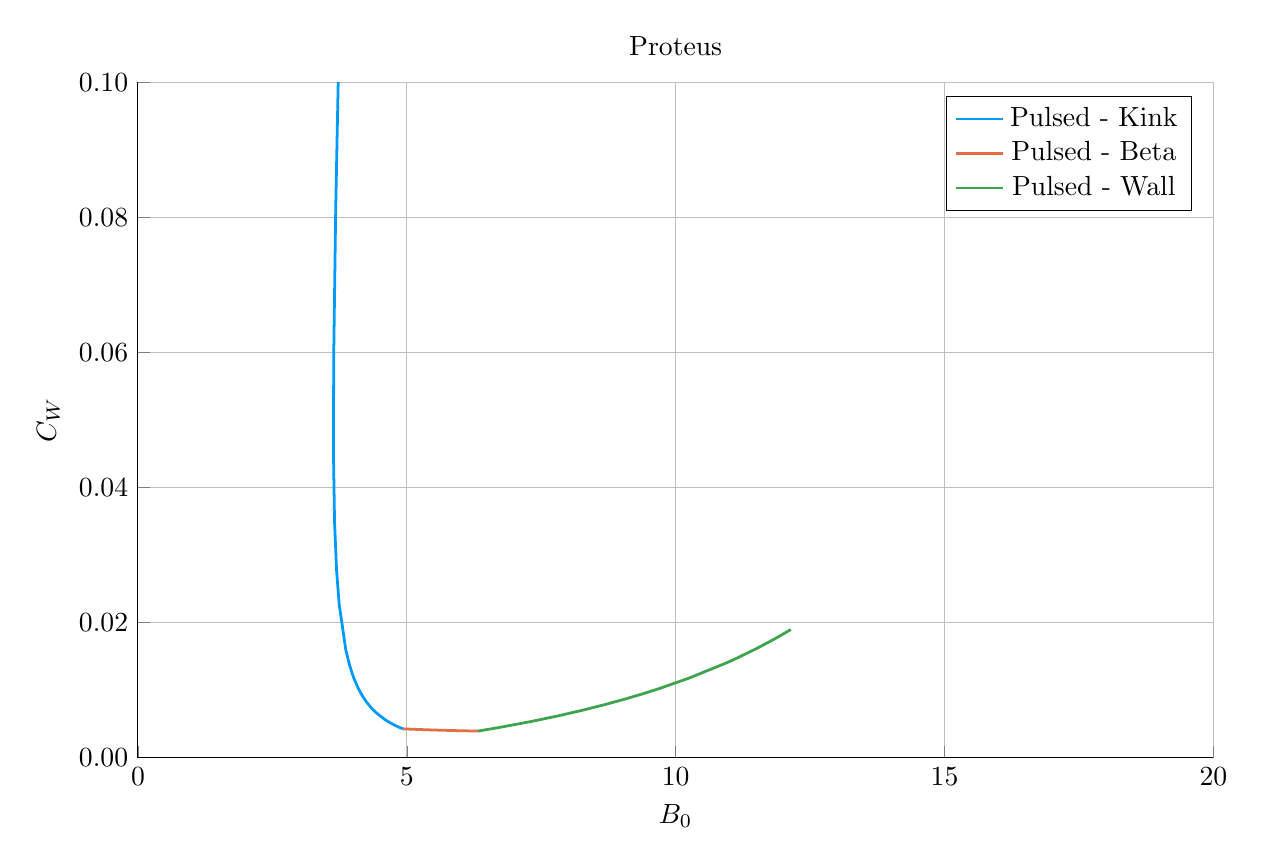
\begin{tikzpicture}[]
\begin{axis}[height = {101.6mm}, ylabel = {${C}_{W}$}, title = {Proteus}, xmin = {0.0}, xmax = {20.0}, ymax = {0.1}, xlabel = {${B}_{0}$}, {unbounded coords=jump, scaled x ticks = false, xticklabel style={rotate = 0}, xmajorgrids = true, xtick = {0.0,5.0,10.0,15.0,20.0}, xticklabels = {0,5,10,15,20}, xtick align = inside, axis lines* = left, scaled y ticks = false, yticklabel style={rotate = 0}, ymajorgrids = true, ytick = {0.0,0.02,0.04,0.06,0.08,0.1}, yticklabels = {0.00,0.02,0.04,0.06,0.08,0.10}, ytick align = inside, axis lines* = left,     xshift = 0.0mm,
    yshift = 0.0mm,
    axis background/.style={fill={rgb,1:red,1.00000000;green,1.00000000;blue,1.00000000}}
, colorbar style={title=}}, ymin = {0.0}, width = {152.4mm}]\addplot+ [color = {rgb,1:red,0.00000000;green,0.60560316;blue,0.97868012},
draw opacity=1.0,
line width=1,
solid,mark = none,
mark size = 2.0,
mark options = {
    color = {rgb,1:red,0.00000000;green,0.00000000;blue,0.00000000}, draw opacity = 1.0,
    fill = {rgb,1:red,0.00000000;green,0.60560316;blue,0.97868012}, fill opacity = 1.0,
    line width = 1,
    rotate = 0,
    solid
}]coordinates {
(4.658732060637907, 0.5238680720960677)
(4.211109766361548, 0.29158377814463826)
(3.9293920326356777, 0.17767190497429325)
(3.7651903683456465, 0.1166072358238225)
(3.6776039543745567, 0.08112372927887979)
(3.6402437753208394, 0.05909652489757084)
(3.6366994671255806, 0.04467306876996977)
(3.656621534643579, 0.03480923074663025)
(3.693300156736026, 0.02781736023114741)
(3.7422515017241134, 0.022710208007687336)
(3.865532743079537, 0.015952709019313158)
(3.936096932264377, 0.013665127664349888)
(4.010907188015084, 0.01184965388633812)
(4.089072356933184, 0.010387577045642686)
(4.169903401491354, 0.009194676609194867)
(4.252857906625248, 0.008210013517334984)
(4.337501757261618, 0.007388710643319612)
(4.42348218754058, 0.006697190814676216)
(4.5983381267510195, 0.005607443376267891)
(4.686766232902671, 0.005174363801875551)
(4.775618142770625, 0.004798727872321348)
(4.864743502376605, 0.004470996685456748)
(4.927312314219091, 0.004265648977267023)
};
\addlegendentry{Pulsed - Kink}
\addplot+ [color = {rgb,1:red,0.88887350;green,0.43564919;blue,0.27812294},
draw opacity=1.0,
line width=1,
solid,mark = none,
mark size = 2.0,
mark options = {
    color = {rgb,1:red,0.00000000;green,0.00000000;blue,0.00000000}, draw opacity = 1.0,
    fill = {rgb,1:red,0.88887350;green,0.43564919;blue,0.27812294}, fill opacity = 1.0,
    line width = 1,
    rotate = 0,
    solid
}]coordinates {
(4.927312314219091, 0.004265648977267023)
(4.984545814413324, 0.004246004028390513)
(5.17452482724068, 0.0041849470602593405)
(5.362091669637646, 0.0041306604637180565)
(5.54700293215903, 0.004082678433657853)
(5.729042482638278, 0.004040568150841258)
(5.908022832274664, 0.004003927180150204)
(6.083785777786694, 0.003972381072297988)
(6.256202341425288, 0.003945581215430235)
(6.324169421042356, 0.003936121998618512)
};
\addlegendentry{Pulsed - Beta}
\addplot+ [color = {rgb,1:red,0.24222430;green,0.64327509;blue,0.30444865},
draw opacity=1.0,
line width=1,
solid,mark = none,
mark size = 2.0,
mark options = {
    color = {rgb,1:red,0.00000000;green,0.00000000;blue,0.00000000}, draw opacity = 1.0,
    fill = {rgb,1:red,0.24222430;green,0.64327509;blue,0.30444865}, fill opacity = 1.0,
    line width = 1,
    rotate = 0,
    solid
}]coordinates {
(6.324169421042356, 0.003936121998618512)
(6.727338549778396, 0.004479602725986452)
(7.320469048424473, 0.005364564868057796)
(7.835746509376305, 0.006224935802002464)
(8.290245520072391, 0.007063234029306885)
(8.696162676727877, 0.00788223849893927)
(9.0624397222742, 0.00868451845222651)
(9.395798186463841, 0.00947231261660997)
(9.701405747258567, 0.010247527923592582)
(10.244760202900984, 0.011766415534875542)
(10.930275827723788, 0.013983337609097824)
(11.131878682735255, 0.014709436843559874)
(11.50278450645086, 0.01614615622924262)
(11.83715172742864, 0.017565397423788643)
(11.992609772603878, 0.018269423189653803)
(12.141110720831467, 0.018970135151011147)
};
\addlegendentry{Pulsed - Wall}
\end{axis}

\end{tikzpicture}

		\end{adjustbox}
        \caption{Proteus Cost-per-Watt}
    \end{subfigure}
    \hfill
    \begin{subfigure}[t]{0.45\textwidth}
        \centering
		\begin{adjustbox}{width=\textwidth}
			\Large
			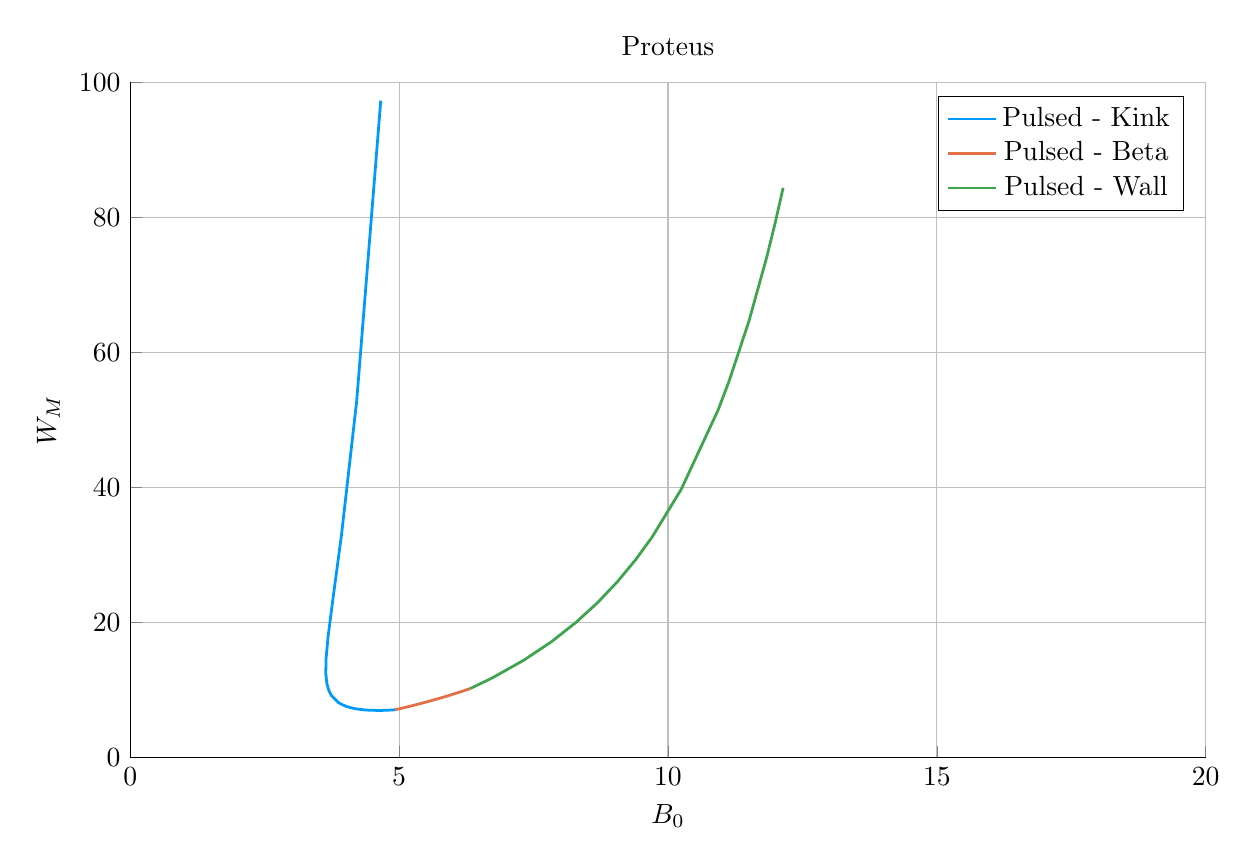
\begin{tikzpicture}[]
\begin{axis}[height = {101.6mm}, ylabel = {${W}_{M}$}, title = {Proteus}, xmin = {0.0}, xmax = {20.0}, ymax = {100.0}, xlabel = {${B}_{0}$}, {unbounded coords=jump, scaled x ticks = false, xticklabel style={rotate = 0}, xmajorgrids = true, xtick = {0.0,5.0,10.0,15.0,20.0}, xticklabels = {0,5,10,15,20}, xtick align = inside, axis lines* = left, scaled y ticks = false, yticklabel style={rotate = 0}, ymajorgrids = true, ytick = {0.0,20.0,40.0,60.0,80.0,100.0}, yticklabels = {0,20,40,60,80,100}, ytick align = inside, axis lines* = left,     xshift = 0.0mm,
    yshift = 0.0mm,
    axis background/.style={fill={rgb,1:red,1.00000000;green,1.00000000;blue,1.00000000}}
, colorbar style={title=}}, ymin = {0.0}, width = {152.4mm}]\addplot+ [color = {rgb,1:red,0.00000000;green,0.60560316;blue,0.97868012},
draw opacity=1.0,
line width=1,
solid,mark = none,
mark size = 2.0,
mark options = {
    color = {rgb,1:red,0.00000000;green,0.00000000;blue,0.00000000}, draw opacity = 1.0,
    fill = {rgb,1:red,0.00000000;green,0.60560316;blue,0.97868012}, fill opacity = 1.0,
    line width = 1,
    rotate = 0,
    solid
}]coordinates {
(4.658732060637907, 97.28232425378617)
(4.211109766361548, 52.81528522659042)
(3.9293920326356777, 33.045940900779435)
(3.7651903683456465, 23.247661382566328)
(3.6776039543745567, 17.827034690374397)
(3.6402437753208394, 14.548456710153735)
(3.6366994671255806, 12.424185075208992)
(3.656621534643579, 10.973706805818463)
(3.693300156736026, 9.943115007776825)
(3.7422515017241134, 9.18863958559583)
(3.865532743079537, 8.195040941316238)
(3.936096932264377, 7.866037710488523)
(4.010907188015084, 7.612872940496481)
(4.089072356933184, 7.418652478460303)
(4.169903401491354, 7.271257368183174)
(4.252857906625248, 7.16179941021134)
(4.337501757261618, 7.083633084260422)
(4.42348218754058, 7.031705491759868)
(4.5983381267510195, 6.991823293679325)
(4.686766232902671, 6.998413622496496)
(4.775618142770625, 7.019967223555443)
(4.864743502376605, 7.054937735216179)
(4.927312314219091, 7.086769144908002)
};
\addlegendentry{Pulsed - Kink}
\addplot+ [color = {rgb,1:red,0.88887350;green,0.43564919;blue,0.27812294},
draw opacity=1.0,
line width=1,
solid,mark = none,
mark size = 2.0,
mark options = {
    color = {rgb,1:red,0.00000000;green,0.00000000;blue,0.00000000}, draw opacity = 1.0,
    fill = {rgb,1:red,0.88887350;green,0.43564919;blue,0.27812294}, fill opacity = 1.0,
    line width = 1,
    rotate = 0,
    solid
}]coordinates {
(4.927312314219091, 7.086769144908002)
(4.984545814413324, 7.193516773221651)
(5.17452482724068, 7.558989804600146)
(5.362091669637646, 7.937858802904825)
(5.54700293215903, 8.330611438237515)
(5.729042482638278, 8.737734587814298)
(5.908022832274664, 9.159710709615348)
(6.083785777786694, 9.597014749238335)
(6.256202341425288, 10.050111620812826)
(6.324169421042356, 10.235766195929495)
};
\addlegendentry{Pulsed - Beta}
\addplot+ [color = {rgb,1:red,0.24222430;green,0.64327509;blue,0.30444865},
draw opacity=1.0,
line width=1,
solid,mark = none,
mark size = 2.0,
mark options = {
    color = {rgb,1:red,0.00000000;green,0.00000000;blue,0.00000000}, draw opacity = 1.0,
    fill = {rgb,1:red,0.24222430;green,0.64327509;blue,0.30444865}, fill opacity = 1.0,
    line width = 1,
    rotate = 0,
    solid
}]coordinates {
(6.324169421042356, 10.235766195929495)
(6.727338549778396, 11.783493156592025)
(7.320469048424473, 14.433662866898274)
(7.835746509376305, 17.179550950209588)
(8.290245520072391, 20.029490714669382)
(8.696162676727877, 22.99147222981706)
(9.0624397222742, 26.07266302814804)
(9.395798186463841, 29.27939084761122)
(9.701405747258567, 32.61725020270231)
(10.244760202900984, 39.70580850721064)
(10.930275827723788, 51.43239308745394)
(11.131878682735255, 55.64715526987581)
(11.50278450645086, 64.55415559202683)
(11.83715172742864, 74.11630708302644)
(11.992609772603878, 79.14953842129572)
(12.141110720831467, 84.35411724014395)
};
\addlegendentry{Pulsed - Wall}
\end{axis}

\end{tikzpicture}

		\end{adjustbox}
        \caption{Proteus Capital Cost}
    \end{subfigure}
    \hfill \hfill ~\\ ~\\ ~\\ ~\\
    \hfill 
    \begin{subfigure}[t]{0.45\textwidth}
        \centering
		\begin{adjustbox}{width=\textwidth}
			\Large
			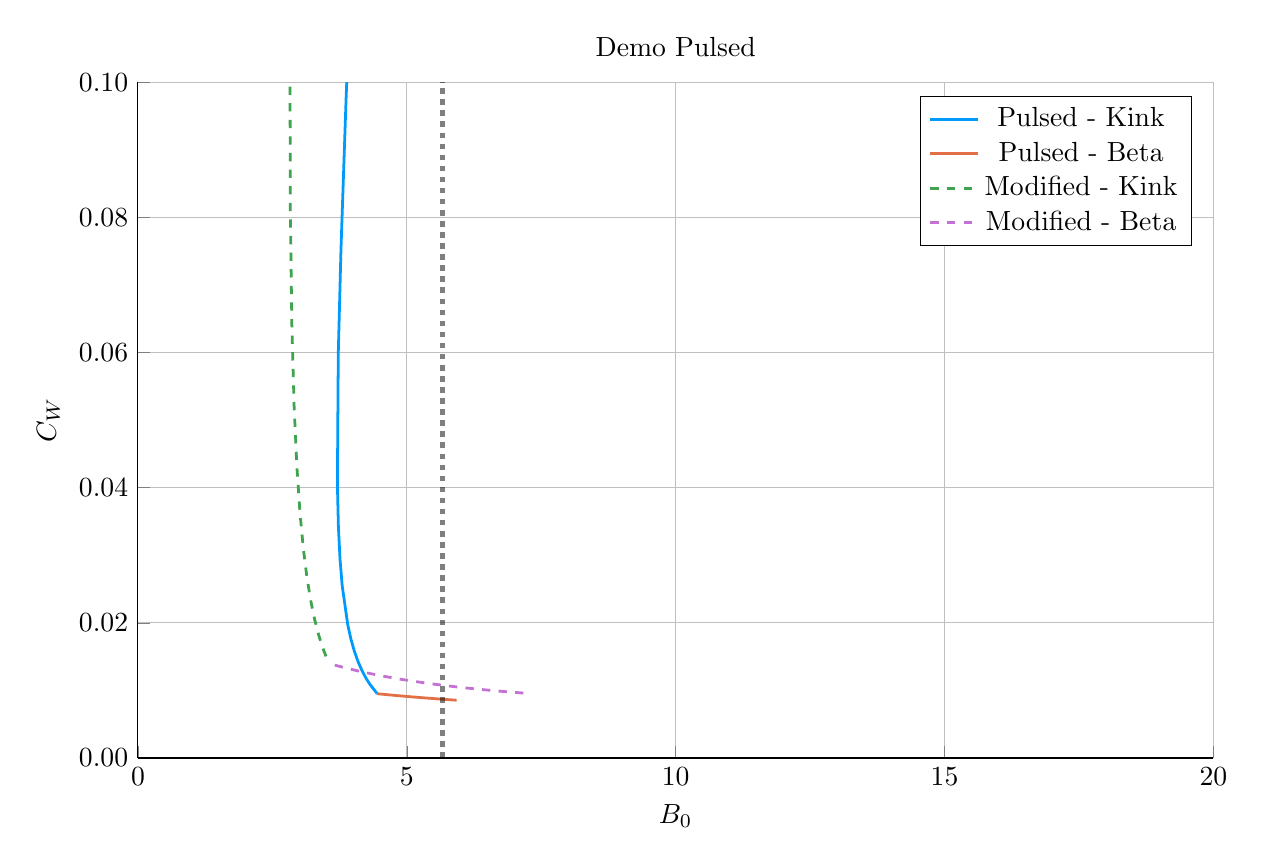
\begin{tikzpicture}[]
\begin{axis}[height = {101.6mm}, ylabel = {${C}_{W}$}, title = {Demo Pulsed}, xmin = {0.0}, xmax = {20.0}, ymax = {0.1}, xlabel = {${B}_{0}$}, {unbounded coords=jump, scaled x ticks = false, xticklabel style={rotate = 0}, xmajorgrids = true, xtick = {0.0,5.0,10.0,15.0,20.0}, xticklabels = {0,5,10,15,20}, xtick align = inside, axis lines* = left, scaled y ticks = false, yticklabel style={rotate = 0}, ymajorgrids = true, ytick = {0.0,0.02,0.04,0.06,0.08,0.1}, yticklabels = {0.00,0.02,0.04,0.06,0.08,0.10}, ytick align = inside, axis lines* = left,     xshift = 0.0mm,
    yshift = 0.0mm,
    axis background/.style={fill={rgb,1:red,1.00000000;green,1.00000000;blue,1.00000000}}
, colorbar style={title=}}, ymin = {0.0}, width = {152.4mm}]\addplot+ [color = {rgb,1:red,0.00000000;green,0.60560316;blue,0.97868012},
draw opacity=1.0,
line width=1,
solid,mark = none,
mark size = 2.0,
mark options = {
    color = {rgb,1:red,0.00000000;green,0.00000000;blue,0.00000000}, draw opacity = 1.0,
    fill = {rgb,1:red,0.00000000;green,0.60560316;blue,0.97868012}, fill opacity = 1.0,
    line width = 1,
    rotate = 0,
    solid
}]coordinates {
(4.327031075670194, 0.1892287825513326)
(4.038214026054326, 0.13206162052102163)
(3.8713719163129245, 0.09770836377510679)
(3.7758613845615545, 0.0753228145367537)
(3.7257856761317214, 0.05989044017674145)
(3.7090473695925437, 0.04055229837333577)
(3.727711597554826, 0.03426367140819575)
(3.7586131667481433, 0.029359319233913946)
(3.799052518631718, 0.025462690957960717)
(3.901290136389271, 0.019741499311841708)
(3.960577465316514, 0.017607284508542168)
(4.0241209645210345, 0.015819330878112364)
(4.0912717805663785, 0.014306863958145555)
(4.161514602943343, 0.013016229386127556)
(4.2344343960723005, 0.0119061698584303)
(4.309692554546368, 0.010944552619225426)
(4.450417240491067, 0.009508186007059894)
};
\addlegendentry{Pulsed - Kink}
\addplot+ [color = {rgb,1:red,0.88887350;green,0.43564919;blue,0.27812294},
draw opacity=1.0,
line width=1,
solid,mark = none,
mark size = 2.0,
mark options = {
    color = {rgb,1:red,0.00000000;green,0.00000000;blue,0.00000000}, draw opacity = 1.0,
    fill = {rgb,1:red,0.88887350;green,0.43564919;blue,0.27812294}, fill opacity = 1.0,
    line width = 1,
    rotate = 0,
    solid
}]coordinates {
(4.450417240491067, 0.009508186007059894)
(4.490148631384312, 0.009477474217304566)
(4.692490181445514, 0.009325449924582748)
(4.8960344619053355, 0.009179881556836224)
(5.100651132702229, 0.00904086745514222)
(5.306202822090688, 0.008908420253381469)
(5.512545696627038, 0.008782491226353)
(5.719530043226767, 0.008662988371093566)
(5.927000883375481, 0.00854978980550123)
};
\addlegendentry{Pulsed - Beta}
\addplot+ [color = {rgb,1:red,0.24222430;green,0.64327509;blue,0.30444865},
draw opacity=1.0,
line width=1,
dashed,mark = none,
mark size = 2.0,
mark options = {
    color = {rgb,1:red,0.00000000;green,0.00000000;blue,0.00000000}, draw opacity = 1.0,
    fill = {rgb,1:red,0.24222430;green,0.64327509;blue,0.30444865}, fill opacity = 1.0,
    line width = 1,
    rotate = 0,
    solid
}]coordinates {
(3.4087424183072135, 0.34025279914240075)
(2.977074181068944, 0.20266043375242454)
(2.8592500074202523, 0.14107963570535767)
(2.827199220063259, 0.10460917631328934)
(2.8339789008667826, 0.08069963800921795)
(2.862412302880871, 0.06408640910554732)
(2.9044598258085443, 0.05207050885933721)
(2.95577893007882, 0.04311069749575431)
(3.0137895352525907, 0.03626387631819784)
(3.076849710218805, 0.03092374739004359)
(3.1438583711612704, 0.02668548743841045)
(3.214045733980633, 0.023270423882766844)
(3.2868548955983727, 0.020481784288090023)
(3.361871149981842, 0.018177576354657807)
(3.4387778750377818, 0.016253383634250513)
(3.5173279629378453, 0.014631131503744007)
};
\addlegendentry{Modified - Kink}
\addplot+ [color = {rgb,1:red,0.76444018;green,0.44411178;blue,0.82429754},
draw opacity=1.0,
line width=1,
dashed,mark = none,
mark size = 2.0,
mark options = {
    color = {rgb,1:red,0.00000000;green,0.00000000;blue,0.00000000}, draw opacity = 1.0,
    fill = {rgb,1:red,0.76444018;green,0.44411178;blue,0.82429754}, fill opacity = 1.0,
    line width = 1,
    rotate = 0,
    solid
}]coordinates {
(3.6607028750648505, 0.013744899135556416)
(3.8574448036470477, 0.013332033203155177)
(4.056375867871351, 0.012949491171136135)
(4.257366397480293, 0.012594759179481692)
(4.460279103534801, 0.012265542491796714)
(4.664969389370631, 0.011959760748489753)
(4.871285596007394, 0.011675536110154509)
(5.07906923307514, 0.01141117796484883)
(5.288155233306219, 0.011165166374807946)
(5.498372259673351, 0.010936135522073528)
(5.709543087166185, 0.010722857854384784)
(5.921485076209294, 0.010524229289897682)
(6.134010749367255, 0.010339255636975386)
(6.346928478632384, 0.0101670402635639)
(6.560043285872518, 0.010006772983002756)
(6.773157754368795, 0.009857720087022352)
(6.986073044284746, 0.009719215441404045)
(7.198590001107076, 0.00959065255201969)
};
\addlegendentry{Modified - Beta}
\addplot+ [color = {rgb,1:red,0.00000000;green,0.00000000;blue,0.00000000},
draw opacity=0.5,
line width=2,
dotted,mark = none,
mark size = 2.0,
mark options = {
    color = {rgb,1:red,0.00000000;green,0.00000000;blue,0.00000000}, draw opacity = 0.5,
    fill = {rgb,1:red,0.00000000;green,0.00000000;blue,0.00000000}, fill opacity = 0.5,
    line width = 1,
    rotate = 0,
    solid
},forget plot]coordinates {
(0.0, NaN)
(20.0, NaN)
};
\addplot+ [color = {rgb,1:red,0.00000000;green,0.00000000;blue,0.00000000},
draw opacity=0.5,
line width=2,
dotted,mark = none,
mark size = 2.0,
mark options = {
    color = {rgb,1:red,0.00000000;green,0.00000000;blue,0.00000000}, draw opacity = 0.5,
    fill = {rgb,1:red,0.00000000;green,0.00000000;blue,0.00000000}, fill opacity = 0.5,
    line width = 1,
    rotate = 0,
    solid
},forget plot]coordinates {
(5.667, 0.0)
(5.667, 0.1)
};
\addplot+[draw=none, color = {rgb,1:red,0.00000000;green,0.00000000;blue,0.00000000},
draw opacity=0.5,
line width=0,
solid,mark = *,
mark size = 2.0,
mark options = {
    color = {rgb,1:red,0.00000000;green,0.00000000;blue,0.00000000}, draw opacity = 0.5,
    fill = {rgb,1:red,0.00000000;green,0.00000000;blue,0.00000000}, fill opacity = 0.5,
    line width = 1,
    rotate = 0,
    solid
},forget plot] coordinates {
(5.667, NaN)
};
\end{axis}

\end{tikzpicture}

		\end{adjustbox}
        \caption{Demo Pulsed Cost-per-Watt}
    \end{subfigure}
    \hfill
    \begin{subfigure}[t]{0.45\textwidth}
        \centering
		\begin{adjustbox}{width=\textwidth}
			\Large
			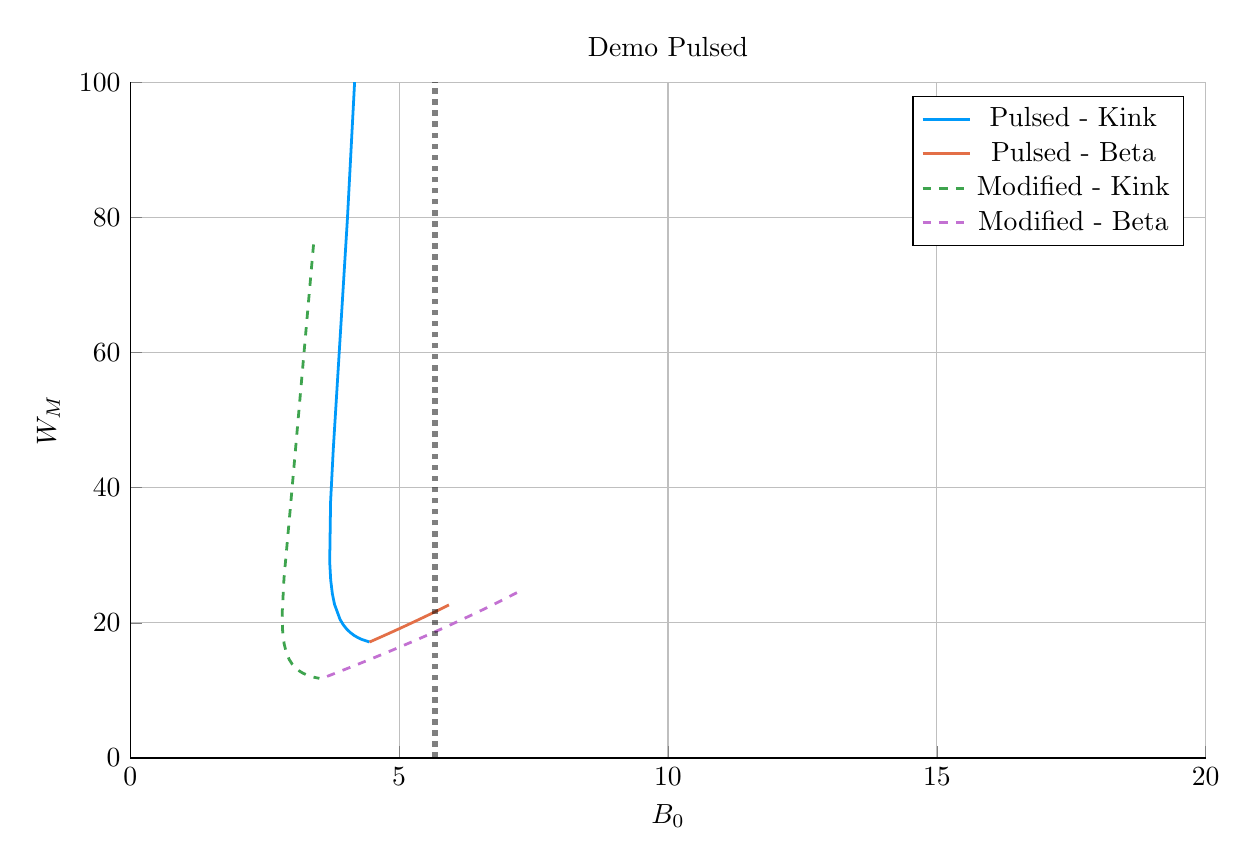
\begin{tikzpicture}[]
\begin{axis}[height = {101.6mm}, ylabel = {${W}_{M}$}, title = {Demo Pulsed}, xmin = {0.0}, xmax = {20.0}, ymax = {100.0}, xlabel = {${B}_{0}$}, {unbounded coords=jump, scaled x ticks = false, xticklabel style={rotate = 0}, xmajorgrids = true, xtick = {0.0,5.0,10.0,15.0,20.0}, xticklabels = {0,5,10,15,20}, xtick align = inside, axis lines* = left, scaled y ticks = false, yticklabel style={rotate = 0}, ymajorgrids = true, ytick = {0.0,20.0,40.0,60.0,80.0,100.0}, yticklabels = {0,20,40,60,80,100}, ytick align = inside, axis lines* = left,     xshift = 0.0mm,
    yshift = 0.0mm,
    axis background/.style={fill={rgb,1:red,1.00000000;green,1.00000000;blue,1.00000000}}
, colorbar style={title=}}, ymin = {0.0}, width = {152.4mm}]\addplot+ [color = {rgb,1:red,0.00000000;green,0.60560316;blue,0.97868012},
draw opacity=1.0,
line width=1,
solid,mark = none,
mark size = 2.0,
mark options = {
    color = {rgb,1:red,0.00000000;green,0.00000000;blue,0.00000000}, draw opacity = 1.0,
    fill = {rgb,1:red,0.00000000;green,0.60560316;blue,0.97868012}, fill opacity = 1.0,
    line width = 1,
    rotate = 0,
    solid
}]coordinates {
(4.327031075670194, 123.44373673332173)
(4.038214026054326, 79.76523284023226)
(3.8713719163129245, 58.108897430981536)
(3.7758613845615545, 45.733304605517155)
(3.7257856761317214, 37.95828264093558)
(3.7090473695925437, 29.04694896379975)
(3.727711597554826, 26.344517979953586)
(3.7586131667481433, 24.306117941226923)
(3.799052518631718, 22.733747168495924)
(3.901290136389271, 20.517766605492294)
(3.960577465316514, 19.728940193613518)
(4.0241209645210345, 19.090733790490855)
(4.0912717805663785, 18.572256162198553)
(4.161514602943343, 18.150497380470465)
(4.2344343960723005, 17.808002600991745)
(4.309692554546368, 17.531315861496644)
(4.450417240491067, 17.166473566094577)
};
\addlegendentry{Pulsed - Kink}
\addplot+ [color = {rgb,1:red,0.88887350;green,0.43564919;blue,0.27812294},
draw opacity=1.0,
line width=1,
solid,mark = none,
mark size = 2.0,
mark options = {
    color = {rgb,1:red,0.00000000;green,0.00000000;blue,0.00000000}, draw opacity = 1.0,
    fill = {rgb,1:red,0.88887350;green,0.43564919;blue,0.27812294}, fill opacity = 1.0,
    line width = 1,
    rotate = 0,
    solid
}]coordinates {
(4.450417240491067, 17.166473566094577)
(4.490148631384312, 17.305309015848636)
(4.692490181445514, 18.019389484737392)
(4.8960344619053355, 18.749800407200777)
(5.100651132702229, 19.496700146051747)
(5.306202822090688, 20.26030213940914)
(5.512545696627038, 21.04087102241869)
(5.719530043226767, 21.83871936060431)
(5.927000883375481, 22.654204785704835)
};
\addlegendentry{Pulsed - Beta}
\addplot+ [color = {rgb,1:red,0.24222430;green,0.64327509;blue,0.30444865},
draw opacity=1.0,
line width=1,
dashed,mark = none,
mark size = 2.0,
mark options = {
    color = {rgb,1:red,0.00000000;green,0.00000000;blue,0.00000000}, draw opacity = 1.0,
    fill = {rgb,1:red,0.24222430;green,0.64327509;blue,0.30444865}, fill opacity = 1.0,
    line width = 1,
    rotate = 0,
    solid
}]coordinates {
(3.4087424183072135, 76.02109466923234)
(2.977074181068944, 36.99469776498375)
(2.8592500074202523, 26.602664601337402)
(2.827199220063259, 21.660862067495565)
(2.8339789008667826, 18.765953821795108)
(2.862412302880871, 16.874407011263102)
(2.9044598258085443, 15.553537101768894)
(2.95577893007882, 14.590024878457532)
(3.0137895352525907, 13.865991589551562)
(3.076849710218805, 13.310773511983673)
(3.1438583711612704, 12.879335564625128)
(3.214045733980633, 12.54157019826116)
(3.2868548955983727, 12.276561049231674)
(3.361871149981842, 12.069311294803374)
(3.4387778750377818, 11.90878112839417)
(3.5173279629378453, 11.786660090388734)
};
\addlegendentry{Modified - Kink}
\addplot+ [color = {rgb,1:red,0.76444018;green,0.44411178;blue,0.82429754},
draw opacity=1.0,
line width=1,
dashed,mark = none,
mark size = 2.0,
mark options = {
    color = {rgb,1:red,0.00000000;green,0.00000000;blue,0.00000000}, draw opacity = 1.0,
    fill = {rgb,1:red,0.76444018;green,0.44411178;blue,0.82429754}, fill opacity = 1.0,
    line width = 1,
    rotate = 0,
    solid
}]coordinates {
(3.6607028750648505, 12.074397140834275)
(3.8574448036470477, 12.685277919648211)
(4.056375867871351, 13.310146449544076)
(4.257366397480293, 13.949057026240864)
(4.460279103534801, 14.602113733589642)
(4.664969389370631, 15.269467629207359)
(4.871285596007394, 15.951314711845848)
(5.07906923307514, 16.647894398080105)
(5.288155233306219, 17.359488308762714)
(5.498372259673351, 18.086419214151615)
(5.709543087166185, 18.82905002156669)
(5.921485076209294, 19.587782712469505)
(6.134010749367255, 20.363057156601585)
(6.346928478632384, 21.155349745799302)
(6.560043285872518, 21.965171804607706)
(6.773157754368795, 22.79306774804729)
(6.986073044284746, 23.639612971086876)
(7.198590001107076, 24.50541146426436)
};
\addlegendentry{Modified - Beta}
\addplot+ [color = {rgb,1:red,0.00000000;green,0.00000000;blue,0.00000000},
draw opacity=0.5,
line width=2,
dotted,mark = none,
mark size = 2.0,
mark options = {
    color = {rgb,1:red,0.00000000;green,0.00000000;blue,0.00000000}, draw opacity = 0.5,
    fill = {rgb,1:red,0.00000000;green,0.00000000;blue,0.00000000}, fill opacity = 0.5,
    line width = 1,
    rotate = 0,
    solid
},forget plot]coordinates {
(0.0, NaN)
(20.0, NaN)
};
\addplot+ [color = {rgb,1:red,0.00000000;green,0.00000000;blue,0.00000000},
draw opacity=0.5,
line width=2,
dotted,mark = none,
mark size = 2.0,
mark options = {
    color = {rgb,1:red,0.00000000;green,0.00000000;blue,0.00000000}, draw opacity = 0.5,
    fill = {rgb,1:red,0.00000000;green,0.00000000;blue,0.00000000}, fill opacity = 0.5,
    line width = 1,
    rotate = 0,
    solid
},forget plot]coordinates {
(5.667, 0.0)
(5.667, 100.0)
};
\addplot+[draw=none, color = {rgb,1:red,0.00000000;green,0.00000000;blue,0.00000000},
draw opacity=0.5,
line width=0,
solid,mark = *,
mark size = 2.0,
mark options = {
    color = {rgb,1:red,0.00000000;green,0.00000000;blue,0.00000000}, draw opacity = 0.5,
    fill = {rgb,1:red,0.00000000;green,0.00000000;blue,0.00000000}, fill opacity = 0.5,
    line width = 1,
    rotate = 0,
    solid
},forget plot] coordinates {
(5.667, NaN)
};
\end{axis}

\end{tikzpicture}

		\end{adjustbox}
        \caption{Demo Pulsed Capital Cost}
    \end{subfigure}	
    \hfill \hfill ~\\ ~\\ ~\\
    \caption{Pulsed Cost Curves}
    \label{fig:pulsed_costs}
\end{figure*}

Summarizing the conclusions of this subsection, the beta limit is usually the best constraint to operate at. For lowering the cost-per-watt, a reactor should always be run at the highest magnetic field strength ($B_0$) that satisfies the beta limit. This most often occurs when wall loading takes over (for steady-state reactors) or reactors start being physically unrealizable (for pulsed ones). Building cheap to build reactors -- i.e. minimizing capital cost -- then actually proved to make pulsed design one of trade-offs. This is because the beta-kink curve intersection produces a low capital cost reactor, but at the price of operating at a subpar cost-per-watt. Designers should therefore balance the two cost metrics.

\subsection{Utilizing High Field Magnets}

The main conclusion for this paper is that high field magnets are the way to go to build an efficient, compact fusion reactor. In line with the MIT ARC effort, these high fields will be built with high-temperature superconducting (HTS) tape. This innovation is set to double the strength of conventional magnets. The real question is how best to use it.

At a very simple level, there are two main places strong magnets can be employed: the toroidal fields ($B_0$) and the central solenoid ($B_{CS}$). The easier mode of operation to start with is steady-state. This is because steady-state tokamaks do not rely on a central solenoid for the profitability of their machines. Further, the cost curves in \cref{fig:steady_cost} show that all these designs would benefit from toroidal fields ($B_0$) not achievable with conventional magnets -- which can only reach around 10 T on a good day.

The more interesting result is that pulsed reactors gain no real benefit from using HTS toroidal field magnets. Within the modern paradigm (i.e. D-T fuel, H-Mode, etc), pulsed reactors never have to exceed the limits of inexpensive, copper magnets. The place HTS can really help is with the central solenoid, which governs how long a pulse can last. Further, the effect of improving the central solenoid saturates within the range accessible to HTS tape. Again, HTS would be more than adequate for the modern paradigm.

\begin{figure*}
    \centering
    \hfill 
    \begin{subfigure}[t]{0.45\textwidth}
        \centering
		\begin{adjustbox}{width=\textwidth}
			\Large
			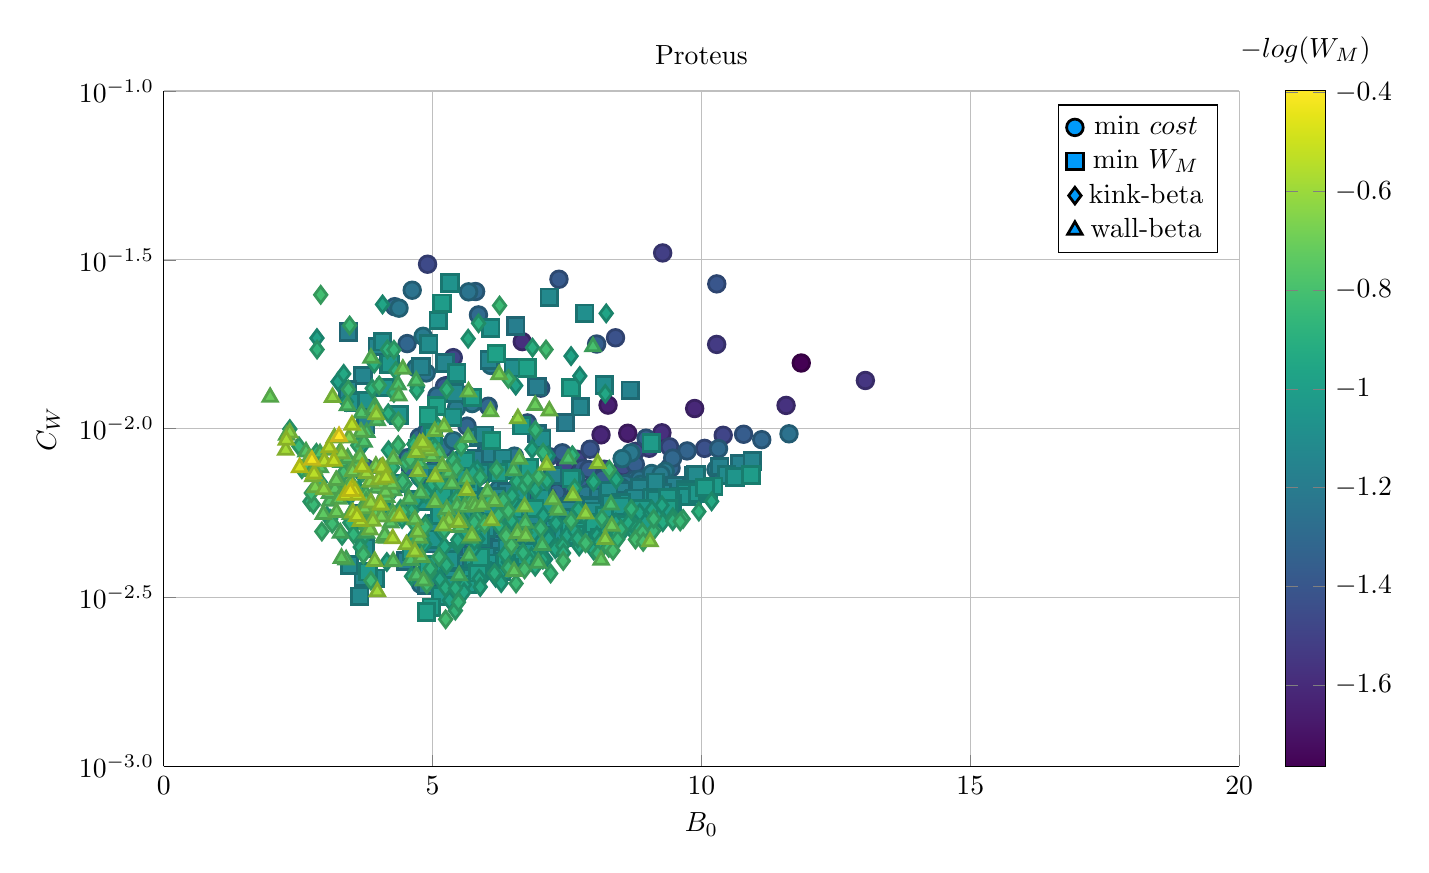
\begin{tikzpicture}[]
\begin{axis}[colorbar = {true}, height = {101.6mm}, ylabel = {${C}_{W}$}, title = {Proteus}, xmin = {0.0}, xmax = {20.0}, ymax = {0.1}, ymode = {log}, xlabel = {${B}_{0}$}, {unbounded coords=jump, scaled x ticks = false, xticklabel style={rotate = 0}, xmajorgrids = true, xtick = {0.0,5.0,10.0,15.0,20.0}, xticklabels = {0,5,10,15,20}, xtick align = inside, axis lines* = left, scaled y ticks = false, yticklabel style={rotate = 0}, log basis y=10, ymajorgrids = true, ytick = {0.001,0.0031622776601683794,0.01,0.03162277660168379,0.1}, yticklabels = {$10^{-3.0}$,$10^{-2.5}$,$10^{-2.0}$,$10^{-1.5}$,$10^{-1.0}$}, ytick align = inside, axis lines* = left,     xshift = 0.0mm,
    yshift = 0.0mm,
    axis background/.style={fill={rgb,1:red,1.00000000;green,1.00000000;blue,1.00000000}}
, colormap={plots}{rgb=(0.26700400,0.00487400,0.32941500), rgb=(0.27794100,0.05632400,0.38119100), rgb=(0.28291000,0.10539300,0.42690200), rgb=(0.28229000,0.14591200,0.46151000), rgb=(0.27619400,0.19007400,0.49300100), rgb=(0.26514500,0.23295600,0.51659900), rgb=(0.25042500,0.27429000,0.53310300), rgb=(0.23360300,0.31382800,0.54391400), rgb=(0.21813000,0.34743200,0.55003800), rgb=(0.20123900,0.38367000,0.55429400), rgb=(0.18555600,0.41857000,0.55675300), rgb=(0.17117600,0.45253000,0.55796500), rgb=(0.15772900,0.48593200,0.55801300), rgb=(0.14618000,0.51541300,0.55682300), rgb=(0.13374300,0.54853500,0.55354100), rgb=(0.12346300,0.58168700,0.54744500), rgb=(0.11948300,0.61481700,0.53769200), rgb=(0.12632600,0.64410700,0.52531100), rgb=(0.15014800,0.67663100,0.50658900), rgb=(0.19109000,0.70836600,0.48228400), rgb=(0.24607000,0.73891000,0.45202400), rgb=(0.31192500,0.76782200,0.41558600), rgb=(0.37777900,0.79178100,0.37793900), rgb=(0.45867400,0.81636300,0.32972700), rgb=(0.54552400,0.83803900,0.27562600), rgb=(0.63690200,0.85654200,0.21662000), rgb=(0.73088900,0.87191600,0.15602900), rgb=(0.81457600,0.88339300,0.11034700), rgb=(0.90631100,0.89485500,0.09812500), rgb=(0.99324800,0.90615700,0.14393600)}, colorbar style={title=$-log( W_M )$}}, ymin = {0.001}, width = {152.4mm}]\addplot+[scatter, scatter src=explicit, only marks = {true}, color = {rgb,1:red,0.00000000;green,0.60560316;blue,0.97868012},
draw opacity=1,
line width=0,
solid,mark = *,
mark size = 3.0,
mark options = {
    color = {rgb,1:red,0.00000000;green,0.00000000;blue,0.00000000}, draw opacity = 1.0,
    fill = {rgb,1:red,0.00000000;green,0.60560316;blue,0.97868012}, fill opacity = 1,
    line width = 1,
    rotate = 0,
    solid
}] coordinates {
(11.855851167264671, 0.015650867313707448) [-1.7651507846396934]
(8.62894306410229, 0.009694646552347688) [-1.652530796858066]
(8.262669569295957, 0.011744038729478485) [-1.647000146345283]
(8.132345586482765, 0.009590177278586947) [-1.6184546481250472]
(9.87352129314419, 0.011474300333025303) [-1.6124908438767973]
(9.26466071494926, 0.00972401084478665) [-1.5828949402967583]
(6.667811597046653, 0.018106858351787505) [-1.577618500437912]
(11.573395463568893, 0.011719738653164523) [-1.56873554690934]
(5.264528343635174, 0.013419897432724169) [-1.5599002750009094]
(13.048135395345042, 0.013892471464509717) [-1.5518482038436605]
(10.282796584070674, 0.017767343192357253) [-1.5302287668791192]
(9.278542294221232, 0.033146306422516245) [-1.5115301730224102]
(7.5044360623009565, 0.007510212646674021) [-1.5013825191439996]
(9.02784009554164, 0.008751202105526691) [-1.4958902811815062]
(8.710683108208965, 0.00816949735167802) [-1.4892617900728689]
(7.687377168804008, 0.008118078139228204) [-1.4884348201277007]
(10.404534949568816, 0.009559158760396884) [-1.4866425610729714]
(5.384524713145202, 0.01623184139531336) [-1.4835478223239928]
(7.472857057569771, 0.007837831837729894) [-1.4780728724015184]
(4.906484287411937, 0.03069401611625924) [-1.4650031348255397]
(7.111580297007043, 0.006765803188842749) [-1.4601242927308113]
(8.773685022223647, 0.008568870415676909) [-1.453691298071198]
(8.545510256202396, 0.007723927816166263) [-1.4489094778079963]
(7.070436548811644, 0.006162431971740805) [-1.432973868001932]
(6.884154096232421, 0.006329451983138475) [-1.4325147285303634]
(9.405921329983288, 0.008839617844718544) [-1.4268866569895065]
(10.057985274469397, 0.008744700190770928) [-1.4268347679685771]
(8.401821549997786, 0.018590297650719324) [-1.4237681445033143]
(8.189937032371649, 0.007587250291191641) [-1.4234658725845162]
(8.234578254729767, 0.007390656211515189) [-1.4109108269606008]
(7.92991212471289, 0.008694085637837138) [-1.4079262096010774]
(6.59839258184741, 0.00634066157530613) [-1.407330123320285]
(10.284931156770094, 0.026840973164111593) [-1.3996791570309395]
(7.3137838143058795, 0.007040053838733538) [-1.3974870797438]
(5.221820332167986, 0.013359280479800206) [-1.3946269662443698]
(7.785957307166937, 0.007634837530984513) [-1.3905305073664083]
(7.069469201177765, 0.006488653571629467) [-1.3895960301339119]
(6.200523563918331, 0.00554611680879456) [-1.381931002288656]
(7.340133149046422, 0.00695131625200887) [-1.3818272949203658]
(7.349866215424601, 0.027704627448181397) [-1.3812563757949996]
(7.351199097200025, 0.00681167564679013) [-1.379699079550137]
(8.120289345307025, 0.006715817539753603) [-1.376650573885692]
(7.90274300232169, 0.00757067906104037) [-1.3758581110553065]
(7.565484576443418, 0.006499559071472007) [-1.375220700855124]
(7.688718501611012, 0.00646934556613389) [-1.3742348635950123]
(7.005633077388933, 0.0063267927368600325) [-1.3713423550361032]
(7.166534585210968, 0.008267480512087599) [-1.370057699317172]
(5.695615872659735, 0.004988896324536347) [-1.3686239973313072]
(6.620180775083285, 0.005540386026064644) [-1.3680076928767484]
(5.712356159098289, 0.005024205798518008) [-1.3672266212882762]
(10.783439028923059, 0.009628839399324697) [-1.3667105305870977]
(6.000471468140266, 0.0050592629231849704) [-1.3651176317240314]
(8.050752136473724, 0.017814080806893125) [-1.3612722200713383]
(8.77043990632116, 0.007840171434328094) [-1.360737823431438]
(7.010340303297389, 0.013182987051350502) [-1.3596008789905631]
(7.295294539644262, 0.006730765435871485) [-1.3568098625263256]
(6.641599582701438, 0.005632641769207446) [-1.3562925407270994]
(6.645748730966029, 0.005613911931897123) [-1.3540300242042478]
(6.054699810485283, 0.005176189759381431) [-1.3527684291391184]
(9.401252816575663, 0.007678792615766904) [-1.3513432280511455]
(5.581708167132495, 0.006888425944911811) [-1.3508742741062625]
(7.803535098905909, 0.006674090356682625) [-1.348444904526092]
(6.76411548346407, 0.010402669872398145) [-1.3482429808137002]
(8.969455503638764, 0.009376571407375644) [-1.3481015746033576]
(5.634510628688515, 0.012583797530216616) [-1.34746159692277]
(8.156032796881272, 0.007115527316776566) [-1.3450418873098828]
(7.056939291922313, 0.006464286011476574) [-1.3449397649071608]
(7.240799475525162, 0.006186516144095541) [-1.344834769873685]
(6.571134452649435, 0.0053864817732829605) [-1.3436955024234147]
(7.4120702527384665, 0.00848434463520388) [-1.3426163725681677]
(5.934011898969639, 0.004938310227983135) [-1.3374912582230194]
(7.37766442956072, 0.006636608478826529) [-1.335539302100867]
(5.026669706190863, 0.007606581585076429) [-1.3352915983538123]
(6.825792187162438, 0.006029019944814239) [-1.331337874103357]
(9.732916904654346, 0.008594819258321628) [-1.3310780697195672]
(5.698038434377145, 0.004728216221281147) [-1.3292068036291638]
(6.854283769326888, 0.005953363383436291) [-1.32828646244698]
(4.7527705925878685, 0.009441137210103956) [-1.3280975618898123]
(6.452485475407575, 0.005079524630506098) [-1.3278697867431468]
(6.6282734062471, 0.005749625528658903) [-1.327757292865828]
(7.362442088263758, 0.006249734903697681) [-1.3253106415861637]
(6.357926345811093, 0.005155209960292018) [-1.3237407060184172]
(9.434691757978365, 0.007650804529712704) [-1.3217246458754282]
(5.945683748997239, 0.004926318213851794) [-1.319376268743699]
(5.716699212704698, 0.004774448071559269) [-1.3182101821558738]
(7.9999703999657505, 0.0066268624262571275) [-1.31770129332637]
(4.526018058829261, 0.017867829271260238) [-1.3171626271127284]
(7.307142270921693, 0.006479743346210051) [-1.3144438328362922]
(5.64022055353738, 0.010177994071422254) [-1.314397397461996]
(11.121291715489328, 0.009279261565995508) [-1.3134452963620502]
(6.890660641840135, 0.005896178522672516) [-1.3126768401499638]
(5.8496112618323926, 0.007223214696135702) [-1.3123916957087167]
(3.755618871416242, 0.007643344629724278) [-1.3117090270675453]
(6.965828665871357, 0.0062843154751196315) [-1.3112976001573549]
(7.132942553696917, 0.006316305209750007) [-1.3102933400586538]
(6.034623082086722, 0.011655743235665423) [-1.3084666426112759]
(9.464190150712176, 0.008181643780093392) [-1.3081739820914746]
(6.735484315816856, 0.005920113041607297) [-1.3081169022767745]
(6.329532230716051, 0.005266304291939928) [-1.3075986397555424]
(6.949512174456946, 0.0056632699287416785) [-1.3038897119548887]
(5.7123865302563095, 0.004515583648974614) [-1.3034916079905217]
(4.588431546307119, 0.00762405310841983) [-1.301506470226052]
(5.8529754306366, 0.021723513711501174) [-1.2978787946122285]
(6.763583440942078, 0.005860560202229156) [-1.297460949292816]
(5.79974352272628, 0.02547444831481485) [-1.2953226778576867]
(4.294506467374343, 0.022974551007964673) [-1.2951062787178942]
(10.317711969577175, 0.008727794605170999) [-1.2946978796261759]
(7.030442720189729, 0.00606442154900928) [-1.293243062455323]
(6.3155245633398005, 0.00478216163852665) [-1.2916316854649297]
(5.594153930448576, 0.004505685536187866) [-1.291573412415986]
(7.0608047385200905, 0.006201757851874389) [-1.2910367642815292]
(8.746159160738731, 0.007056272547770033) [-1.2894268757747884]
(5.790961836119614, 0.004812007322004063) [-1.2891780169645117]
(7.13931972393237, 0.005900795309436559) [-1.2883016772579983]
(5.642350264315365, 0.004575860387174974) [-1.2877120777365891]
(5.500511487756749, 0.007501625869556503) [-1.2825608117529994]
(5.1870060839860015, 0.004048206616482656) [-1.2803416949249293]
(5.0793762257146975, 0.012501014524680899) [-1.2790944723531177]
(4.900710067477188, 0.009849033693022476) [-1.2789599032268324]
(5.416336002756713, 0.004266328381972482) [-1.278637308935949]
(7.047880217226236, 0.00602317781329061) [-1.2752962713941192]
(4.537987048593646, 0.008202673797589401) [-1.2724318730764337]
(6.7947527911354095, 0.005313590913225172) [-1.26778944603233]
(7.547856502776895, 0.005746237915345085) [-1.2652894696394015]
(8.337373800803634, 0.0063394092295352205) [-1.263844406219344]
(5.839234828237175, 0.004670640784960837) [-1.2622412045786418]
(6.307588148065544, 0.005025369604276285) [-1.2622057750392766]
(6.369182324037021, 0.004715175023029078) [-1.2568407944078956]
(7.25221896281004, 0.005515822538041083) [-1.2564369672634057]
(5.207422458409709, 0.008763742702873716) [-1.255580803936347]
(8.846964102011665, 0.007090160917314494) [-1.2542825781236586]
(11.62801313878366, 0.009658252430988482) [-1.253606675738751]
(6.586437041421525, 0.005078101074449218) [-1.2533258835374417]
(5.896819232149536, 0.004668333949768413) [-1.252740293490489]
(7.218625057420257, 0.005623439530060779) [-1.2512906609771755]
(4.770007649977626, 0.007192663750971734) [-1.2505906665339703]
(6.391248250395476, 0.004753912504004936) [-1.2505667349102745]
(6.722228809625436, 0.00547669175115548) [-1.2505409706978425]
(5.9975644347104575, 0.008585550973626429) [-1.2504311283223648]
(6.220483255591395, 0.00536142422310656) [-1.2495193060816674]
(7.131398255569569, 0.005891517799670805) [-1.2472203996667584]
(4.620896334693883, 0.025703839631456088) [-1.246340221801285]
(5.634708074324937, 0.004426672964739238) [-1.246337044553182]
(6.0053836269885, 0.004733745531528537) [-1.2444533586241864]
(6.122472771064873, 0.004373459187272198) [-1.2410504069560844]
(4.881468969197191, 0.014622918962551527) [-1.2404616678069278]
(5.669873863181108, 0.025422666134658947) [-1.2402101811954278]
(9.159921449108527, 0.00699405114862055) [-1.2399625556579728]
(6.619988989498716, 0.005459593535350185) [-1.2395775558220574]
(4.0721743569002395, 0.006780135026174841) [-1.238968027160994]
(8.487125648729805, 0.006381273355008305) [-1.2381935518916032]
(5.785136288326493, 0.005454977773134567) [-1.2372164242860222]
(7.805870043590986, 0.006162937475975255) [-1.2359322527835273]
(6.521775930847536, 0.008295248979234676) [-1.2345953253761524]
(7.299795216034374, 0.005661235915534237) [-1.2333782101635051]
(6.654376116038794, 0.005116145429327062) [-1.2329256482335589]
(8.586321868785943, 0.0068738253515159406) [-1.2318041138227]
(5.871716076416853, 0.007759607253139788) [-1.2286780396839752]
(5.525881431830733, 0.004270512991179436) [-1.225800447150557]
(4.37566370657649, 0.022744869820021597) [-1.2237626122718148]
(5.386416012885563, 0.009221148903357415) [-1.2192315569877235]
(5.735606858683557, 0.011868028475244749) [-1.2191811590789894]
(8.68706974133124, 0.008481483201532794) [-1.2185680785343938]
(8.63032181590475, 0.00622802822970762) [-1.2179132583990178]
(8.508158073563377, 0.006703260233628488) [-1.2171472173843672]
(7.953691408978824, 0.00633213628058925) [-1.2167448502658762]
(6.081331959057098, 0.015392818825938645) [-1.2162995250149307]
(5.225401290559421, 0.003872910530196867) [-1.215703789534109]
(5.988978974443945, 0.004720977485089404) [-1.2156312790675603]
(9.073087462786646, 0.00736963569440644) [-1.2145283350978044]
(7.217725198328268, 0.005383150867826381) [-1.214317974252912]
(5.536577745729214, 0.004178935326843822) [-1.2138536176262873]
(4.776559777248383, 0.0034641548226198885) [-1.2119360055173332]
(5.211688187540344, 0.0038140534914709043) [-1.2104347246988538]
(10.269380266980404, 0.007570292211977012) [-1.2084631186053005]
(6.918845939903695, 0.0052385995930077645) [-1.2083264519217767]
(7.0692693982238906, 0.005083028024589718) [-1.2073346872626274]
(5.874112036399968, 0.004039129704078142) [-1.2071975929322125]
(4.690082401892927, 0.01513911751066285) [-1.2067840670536927]
(7.861161945792819, 0.006395373245847939) [-1.206736577191552]
(9.326423266814658, 0.007483645463069493) [-1.2065799786199445]
(8.029413669351802, 0.005698374888186277) [-1.203843641047789]
(6.959732144718079, 0.005550896360654382) [-1.203724365314369]
(6.960477287319412, 0.005010777712400389) [-1.2024406864855146]
(7.654476699386534, 0.007157947201399507) [-1.2021169810907544]
(4.823547237227045, 0.01877759730610099) [-1.2015933815507112]
(6.062862639710857, 0.004489267037355289) [-1.2014423796656961]
(8.999102001729389, 0.006374667856956503) [-1.2011965112492808]
(7.2717504340335415, 0.00572395742880883) [-1.2005427289121806]
(6.227413325881237, 0.0066192080125215165) [-1.1994215784439877]
(9.247503176233229, 0.007316062816603203) [-1.1975084180232178]
(5.443249511926066, 0.011502671870448664) [-1.1972619972446426]
(6.742357647461489, 0.005266662336518346) [-1.1967371969067386]
(5.926964832086266, 0.004368135902166705) [-1.1965134818457024]
(8.524769827029726, 0.008154332104698897) [-1.196084536648355]
(8.867575034400405, 0.006843978332329513) [-1.1943424204563022]
(6.457339766119646, 0.005029914775543452) [-1.1908054127888088]
};
\addlegendentry{min $cost$}
\addlegendentry{min $W_M$}
\addlegendentry{kink-beta}
\addlegendentry{wall-beta}
\addplot+[scatter, scatter src=explicit, only marks = {true}, color = {rgb,1:red,0.00000000;green,0.60560316;blue,0.97868012},
draw opacity=1,
line width=0,
solid,mark = square*,
mark size = 3.0,
mark options = {
    color = {rgb,1:red,0.00000000;green,0.00000000;blue,0.00000000}, draw opacity = 1.0,
    fill = {rgb,1:red,0.00000000;green,0.60560316;blue,0.97868012}, fill opacity = 1,
    line width = 1,
    rotate = 0,
    solid
}] coordinates {
(7.4724590738720655, 0.010422279639263054) [-1.1890033537880158]
(6.938996985119089, 0.009658294464102987) [-1.1883675827161198]
(6.9393893920794385, 0.013313745665171912) [-1.1879538738656286]
(6.377850385556073, 0.006487414571263668) [-1.1878029685724296]
(6.547487324963764, 0.020145877705477357) [-1.186260879134981]
(8.029613686159495, 0.005801884747670386) [-1.1859242026174677]
(5.6874025972941205, 0.004217349677698315) [-1.183889066210908]
(7.827309596895398, 0.0058827996938258294) [-1.1830291222504283]
(5.8219713598117036, 0.008160599297710009) [-1.1826268505607591]
(6.946718058585209, 0.004857174007518612) [-1.182365307189366]
(3.434094114791118, 0.01935279381255584) [-1.1822251925764147]
(6.23809783755075, 0.00447855648592392) [-1.1813612663460882]
(5.88781791976068, 0.00428725320402622) [-1.1785285195809967]
(4.505121226933233, 0.004053651772674214) [-1.1775655951090325]
(6.553162158329651, 0.005121496915389368) [-1.17705398157876]
(5.8303432949169745, 0.005890819973806921) [-1.1767452937515073]
(8.807822926389145, 0.006104718148251412) [-1.1766083315756861]
(4.18691738643155, 0.01556268699280997) [-1.173888237216638]
(7.55203601905607, 0.005882961839613334) [-1.1734465174435744]
(5.819836385827624, 0.005961179911412564) [-1.1729466514857931]
(9.116693027577789, 0.006287276174883399) [-1.172839252676928]
(3.659189590525744, 0.005599267038542826) [-1.1727769211527406]
(7.004035835152084, 0.005070632392189801) [-1.1727372361954858]
(4.897086463141796, 0.003434292526080427) [-1.1726542785062386]
(8.087708955601924, 0.0062657093568900535) [-1.1703764252048678]
(6.7024429891400565, 0.004942047034638912) [-1.1699166462753263]
(5.893015258208656, 0.004183590560340062) [-1.1681831393061217]
(7.479710666339309, 0.005170881199231806) [-1.1671080842733117]
(9.508375514310952, 0.006777996547666784) [-1.1655606692177785]
(6.075560203652315, 0.008402469668507205) [-1.165303541813206]
(6.61932998550545, 0.004666935296152095) [-1.1643973078802388]
(6.286558265163782, 0.004663766235492665) [-1.1632535008384055]
(5.050068824721165, 0.004566940606242733) [-1.1631989573193973]
(7.688714523679582, 0.0054331000812183365) [-1.1630392685982025]
(8.505800422917172, 0.006544368204474158) [-1.1625753891662707]
(8.975209897762664, 0.006511116933487475) [-1.1617936783337066]
(8.380983437312786, 0.006126048639979384) [-1.159367616011031]
(8.67470730810651, 0.012995381528200805) [-1.1593260324319568]
(5.960621269295445, 0.004013416769217783) [-1.1592024857112633]
(6.282535161243701, 0.004530529794416821) [-1.1590403977294572]
(10.712436821713085, 0.007867971330715704) [-1.1589428109110296]
(7.099415207654768, 0.005330271588661515) [-1.158451320077056]
(10.3395352744249, 0.007724720119696045) [-1.157468772898154]
(6.536306152444655, 0.004436262085616985) [-1.1570637161067505]
(9.855000808062698, 0.007249642226094706) [-1.1563966451418943]
(5.856384724795581, 0.009420901412013665) [-1.1561531921827275]
(7.454679880823048, 0.0057898611640113395) [-1.1538328200442942]
(5.14753239685863, 0.007237376261288284) [-1.1525173430901554]
(6.856563325018079, 0.004881019954742076) [-1.1522162283529644]
(7.618840457764884, 0.0059379940430840635) [-1.151968932860403]
(8.398440991699191, 0.0061407721476487214) [-1.1511586507355254]
(4.781165601129724, 0.015255960449664327) [-1.1509834966159156]
(6.247011281135245, 0.004419080970160178) [-1.1503660387736743]
(3.7553680100049234, 0.01032617135589161) [-1.1500086948877408]
(5.5152996897670015, 0.004014883666259908) [-1.1494080253790357]
(7.800728278542519, 0.005291422749753008) [-1.1493093072503229]
(6.054088477025007, 0.01598351560152435) [-1.1489823622220707]
(5.411295562966824, 0.003915099463846501) [-1.1484511044037433]
(7.052045109627868, 0.005020529922825154) [-1.1483999797493492]
(5.28488049549897, 0.0034947010100993764) [-1.147064765638366]
(7.62011089503286, 0.005859550653426385) [-1.1465028274549764]
(7.468210164743146, 0.005641165149475234) [-1.144883586902141]
(5.595946792423691, 0.007176119328254024) [-1.144368544047569]
(10.943656185786155, 0.00802165691682325) [-1.1435280806157744]
(7.908061023064291, 0.005447269817044685) [-1.1433393449411435]
(8.854582349908517, 0.006668732693209443) [-1.143332108158641]
(6.549837080949351, 0.004886014774808058) [-1.143184585873657]
(3.9729755898485215, 0.017515494611674454) [-1.1428249654095861]
(3.703954177548893, 0.014377117697389604) [-1.1427984862828113]
(3.4213090828497417, 0.013005276311642224) [-1.142397010267489]
(6.02709699747974, 0.005929095379259443) [-1.1423708774410877]
(5.231750077921478, 0.01565086593371781) [-1.1422424769576425]
(7.2349136535832095, 0.007266091038483963) [-1.140012696356206]
(7.647205004097057, 0.005840600330748377) [-1.1399465227440013]
(6.532016233135844, 0.00480284773560221) [-1.1387943392990294]
(7.523885505796154, 0.005752426766742318) [-1.1382802201938975]
(7.750130276532692, 0.011612930840038163) [-1.1380314198362265]
(9.276469763067444, 0.006446360072583165) [-1.137892443914052]
(5.952941013085345, 0.009562541252399106) [-1.1311113631375915]
(7.951426521304668, 0.005743536904522906) [-1.1302954325651586]
(5.952653119927932, 0.0041760314888273755) [-1.1295543261638465]
(8.253192497448524, 0.006161648966500728) [-1.129462828049983]
(5.512192429439468, 0.00369116854025651) [-1.1277963061708562]
(6.180741676638315, 0.006278926396423389) [-1.126807171194116]
(6.608627477861355, 0.004487529275565533) [-1.1267021554022474]
(9.14457555501132, 0.006938744439971839) [-1.1265761162904897]
(5.310301950330671, 0.004304336836767321) [-1.1261385034152473]
(7.969320198807478, 0.005917258047258142) [-1.1260458936236624]
(7.954215183655014, 0.005885263457738176) [-1.1250537668582923]
(6.771595293849517, 0.005616858230043609) [-1.124511019242948]
(6.641944516873176, 0.004843731890681865) [-1.1236988869720232]
(6.896134858333351, 0.005173923137495115) [-1.1235064786985465]
(3.7132325707792995, 0.003624821435760545) [-1.1232730371267585]
(4.936839162331792, 0.007429853985811719) [-1.1231293548483412]
(6.555316024199809, 0.005231942783984398) [-1.1209978185544383]
(6.304604592673814, 0.008169617815892689) [-1.1196911148335087]
(8.737416781995437, 0.0061580609115664325) [-1.1194748634113345]
(6.123815672401932, 0.004188882178419093) [-1.119418152841014]
(8.324353852438948, 0.005791769416647159) [-1.1191123923650526]
(6.830685941792606, 0.004931972266091366) [-1.1181736482095217]
(8.279157421008941, 0.005611347227289511) [-1.1176702646643628]
(7.172394160745635, 0.024480989089009208) [-1.1175403888423328]
(6.753756430979739, 0.004518885765871233) [-1.1174827013795072]
(8.76524294869496, 0.0062233325455323925) [-1.1174414411464733]
(5.952289891041446, 0.006299808378708293) [-1.1171134960728113]
(6.523754565443294, 0.004568184715721437) [-1.1171111976535804]
(5.4096290381473375, 0.012757776435747556) [-1.1168806186241906]
(9.896916686410892, 0.007305420869085463) [-1.1160945644374545]
(8.286804128590813, 0.005340773800773009) [-1.1139896885893594]
(5.399012890266871, 0.0036233885329560954) [-1.1123768792739945]
(8.296167355721272, 0.005311493039288053) [-1.1112153482766423]
(6.778775360762903, 0.0045000578497955725) [-1.1111283014916062]
(3.642453456441478, 0.003188662256079057) [-1.1108869662710774]
(6.918579935305505, 0.004842654136629077) [-1.1089922492653659]
(6.5071710234613676, 0.00452032863173795) [-1.108391782497311]
(7.258592477367294, 0.00535669926333167) [-1.1082929384878708]
(6.6776055936353265, 0.004745534590751309) [-1.1074346113685616]
(5.3226296796509205, 0.004323464728471098) [-1.1074227437950106]
(10.46985584146923, 0.007293078759243216) [-1.1069130893453907]
(3.4547855533452156, 0.003945456212149148) [-1.106325178133445]
(7.57975455174028, 0.004982808461571556) [-1.1060035644106432]
(5.06842585608741, 0.0052409052861536465) [-1.1038776732161713]
(5.698043204630489, 0.0065314531396132094) [-1.10351060592976]
(7.734654274692709, 0.005173060010686301) [-1.1022315889718237]
(6.228402773452205, 0.005951424789746293) [-1.1016702257969113]
(5.288893434740895, 0.007437806150470808) [-1.100448826904311]
(7.254453932047169, 0.005288339533793414) [-1.0998565094908217]
(6.807046489565401, 0.004337170224988449) [-1.0995498480529582]
(8.496667761878552, 0.005750254423520601) [-1.0992970719713648]
(6.506723144546308, 0.004423364554484401) [-1.0987351440216522]
(8.273277101596172, 0.006535275113176343) [-1.0983869460625248]
(7.024499917691516, 0.006822630998366228) [-1.0977261444257258]
(4.929559505548113, 0.017828562633364364) [-1.0969882385788774]
(6.546519891753608, 0.004407786879742766) [-1.096807077081938]
(6.299458688060015, 0.0041501216036249275) [-1.0962033310727437]
(5.917588131126826, 0.003972749736578854) [-1.0948458082881816]
(6.5027787367036485, 0.015155543307471772) [-1.093965318294314]
(8.191093731826841, 0.013471957430229371) [-1.093275686079877]
(5.765417917352738, 0.003923510470624812) [-1.0931318196649105]
(4.067683728143941, 0.01811006730780237) [-1.0926393639694263]
(5.643295069658257, 0.005671433069083637) [-1.09199330517098]
(5.33448260992027, 0.0035546432563184145) [-1.0916603258728452]
(5.996010919360583, 0.005082501155756355) [-1.091508438458307]
(6.130249778803564, 0.003922207642532424) [-1.0911853630489914]
(5.152309500808404, 0.007129588907950501) [-1.0896526200520398]
(6.613976143688219, 0.004468466025444819) [-1.088663441639713]
(7.828710312153846, 0.021949864805969728) [-1.0877780715734315]
(7.029871400370792, 0.009322832924906896) [-1.0870739196827126]
(6.6598420793586, 0.004672088916974179) [-1.0855818982110972]
(6.33097870945106, 0.004039319528471343) [-1.0844715994400023]
(7.702268833143657, 0.0053439960085053) [-1.0842780595786392]
(6.084754710909704, 0.005760793758021615) [-1.084266572782003]
(7.98999393987453, 0.00569380985136289) [-1.0839928767281124]
(5.068992476376386, 0.0039349920083461085) [-1.0828594792618813]
(9.086048642306793, 0.0062405207423892875) [-1.082853352734588]
(7.44906676523106, 0.0054577800846403015) [-1.0824719035597]
(5.375575122544495, 0.0035809652689903063) [-1.0824709528228211]
(7.386984140765724, 0.005148297391297789) [-1.0814366033908964]
(9.702271536107535, 0.006582162000449632) [-1.0809878234039578]
(9.614854186704672, 0.006301853688415234) [-1.0808972954130593]
(4.645688111866446, 0.006161790226168522) [-1.0797863646031054]
(3.927334262139488, 0.0036086053477567665) [-1.079163153355685]
(6.963971610592974, 0.004793357206410555) [-1.0780309855478056]
(8.244956752748422, 0.0054298508521766365) [-1.076806285491668]
(5.769697532800943, 0.00604411217248383) [-1.0765985094568509]
(7.283344319549832, 0.004828662165485411) [-1.0760641298404754]
(5.392578394594405, 0.005661819547798889) [-1.0757730303287785]
(3.7434225317786316, 0.00443044659495794) [-1.0744056068515366]
(7.7252366425534715, 0.005467468655559742) [-1.073726482715373]
(8.506016241294386, 0.006046667097602973) [-1.072815333291583]
(5.722077224788854, 0.006315687038558954) [-1.0718638391063322]
(3.5290681872248832, 0.011989877345034696) [-1.0710072465261937]
(5.408389828424612, 0.006287200186056995) [-1.0706716976099708]
(5.880603880610476, 0.00739594343637032) [-1.069478881808043]
(3.770984054785403, 0.012080600310741674) [-1.0679830462657767]
(9.144669371614333, 0.006138341400017388) [-1.0670572282884458]
(5.3325423351198395, 0.004085658341340117) [-1.0667391835901658]
(8.316799187366927, 0.006004004929014098) [-1.066302608545655]
(6.389619437625667, 0.004440975162005993) [-1.064104157833971]
(5.324355765249537, 0.026972932068461592) [-1.0640878812065675]
(6.511622532652898, 0.004395996587917252) [-1.0635820925869255]
(6.911249511094287, 0.004423420241739423) [-1.062988318250961]
(7.502962627592097, 0.00480727122317776) [-1.0628036997189863]
(5.469724443246719, 0.0034131330547271113) [-1.062700357913494]
(5.706475165604361, 0.0036974585830479817) [-1.0626514373993834]
(7.276669037534987, 0.004776499853086686) [-1.0610739421064752]
(6.526975357350624, 0.004144297606935685) [-1.0588352037418618]
(5.105089902831069, 0.0209014980088616) [-1.0585986545827941]
(4.374531653432859, 0.010988948677442597) [-1.057135771526312]
(4.122473679442906, 0.013241941603829825) [-1.056315661795303]
(6.078673477412938, 0.019862106250452566) [-1.0562734967702754]
(7.427558910001991, 0.004858658731965693) [-1.0561257856094448]
(7.01015270925273, 0.006223828461257365) [-1.0559814704124602]
(5.014809023336614, 0.004706089102701761) [-1.0555859489072712]
(6.029077134394886, 0.003994614402213268) [-1.0549803415205259]
(9.718000396033032, 0.006463993798881436) [-1.0545713902023608]
(5.896086527792721, 0.0038990516235787613) [-1.054205756099488]
(10.62632239203378, 0.007195479612398366) [-1.0536290024409787]
(9.830251746280974, 0.006286763322784177) [-1.0533216125601341]
(5.653429182632709, 0.004822724612666477) [-1.0529307720930816]
(7.148582094551358, 0.005656264568736301) [-1.0525850668019536]
(9.721783343528084, 0.006295530789348686) [-1.052552508886994]
(6.4747129291886205, 0.007550888758433211) [-1.0509835312174363]
(7.5553171987129115, 0.004904482654727138) [-1.0508250621973283]
(5.689433662550519, 0.006571304536184572) [-1.050680345054969]
(6.819358408267933, 0.004560195418506711) [-1.0506245233592775]
(5.372500908480495, 0.01080264515897382) [-1.0505217359121972]
(9.464104357867244, 0.00597835329976134) [-1.049317623712287]
(9.421645636318559, 0.00605275476812188) [-1.0490747591885061]
(6.83923495211403, 0.004511808104116367) [-1.0489907539423449]
(7.595014509377157, 0.0049153150140211965) [-1.0478434867034416]
(6.9492853284169565, 0.004616652674773231) [-1.0473758850488442]
(6.631954997333512, 0.006447737760929581) [-1.046767629611379]
(4.836574702453568, 0.006114416229637186) [-1.0460742739305466]
(5.447392742867525, 0.01461141466329314) [-1.0428746875530057]
(5.278008805745069, 0.0034297894059699906) [-1.0409932776852704]
(6.869290933859089, 0.004324846597058025) [-1.040720375777512]
(4.388359570069462, 0.0068957525832947) [-1.0400494553390642]
(7.730136216039545, 0.0047742837106654985) [-1.03963800286999]
(5.097390647393597, 0.0070972253563865) [-1.0394862991533038]
(5.705197239891871, 0.006107051538135721) [-1.0391370640013136]
(4.211114439903267, 0.015503036624972183) [-1.038354289214968]
(9.925180494788561, 0.006445735380428859) [-1.0380750082543837]
(8.392824243874195, 0.005205902574339689) [-1.0370263081612092]
(7.973811270774484, 0.005283195240312258) [-1.0365321066837632]
(8.49921904371083, 0.005892181423629392) [-1.0364145571368009]
(6.655649338522086, 0.010214094301379546) [-1.0358730287795153]
(6.272206414918943, 0.003781581128188247) [-1.0352797650690977]
(9.40142074331525, 0.0061316127141858145) [-1.0352425491421158]
(4.6061758509773245, 0.004345014451914255) [-1.0335536367675167]
(5.764426452876033, 0.00415632052734694) [-1.0319535365225938]
(9.372888478292797, 0.006253917955260214) [-1.031638330454266]
(5.729013310777877, 0.003613822408322808) [-1.0316283345953763]
(5.883030813164119, 0.00478160347928963) [-1.0312630056422283]
(6.556479558238363, 0.004326998549376461) [-1.030801418278412]
(6.395724956994062, 0.006039359373565179) [-1.0301227610636083]
(5.139256557257989, 0.005550817437725965) [-1.029015666765989]
(10.123332193763748, 0.006583295742064639) [-1.0288573869793878]
(6.568561456688728, 0.004204292638824563) [-1.0245024368116802]
(5.6039086370880105, 0.007145400138218064) [-1.0231385619546913]
(7.648719554707365, 0.004789677204757558) [-1.021449027000752]
(10.226601060349507, 0.00675373673736514) [-1.0213127693885564]
(5.153470412653239, 0.003193542226257652) [-1.0209276741398987]
(7.579001576207003, 0.007121099635585821) [-1.0202684704954939]
(3.8015765702844804, 0.0037708668397859442) [-1.0187837906200732]
(8.894908266877893, 0.005805595496214904) [-1.0179738483919518]
(9.066566182501706, 0.009070154520460257) [-1.0169425110693646]
(8.213444606213486, 0.00501503870041615) [-1.0162045101447212]
(10.062564168396998, 0.00670010251636303) [-1.0149810946438107]
(4.727731778507776, 0.008752580219573484) [-1.014353466976016]
(5.174769297851055, 0.023528952793841592) [-1.0140528730661398]
(8.195915051921629, 0.005527004085356763) [-1.0133093427968076]
(7.054369905297556, 0.004778958682375364) [-1.0128360857902137]
(5.031848935370691, 0.003842216867194081) [-1.0126834015105255]
(10.922140692684003, 0.007300503854095673) [-1.0124869131348806]
(5.915584448350069, 0.0038089628255598917) [-1.0084966915198963]
(5.602678326023923, 0.008048423371546378) [-1.005776006726422]
(7.544600594243294, 0.005136336479510988) [-1.0027757315503723]
(4.977942341177753, 0.0029594317443149176) [-1.002422823826331]
(5.642218938318191, 0.003459304695059543) [-1.0023352556688647]
(8.295019648678474, 0.004988217345842403) [-0.9994656987080655]
(7.070940189155582, 0.004649343635980374) [-0.9991953302395459]
(6.226711465325763, 0.007411548557741582) [-0.9991876183275935]
(6.419292049664728, 0.0038831217844692545) [-0.9971256954762724]
(4.887255844769486, 0.0028654321699102935) [-0.9968293366364798]
(7.7523402111694955, 0.004992975570566671) [-0.9965130838642419]
(5.890289877584987, 0.003830578946172306) [-0.9960911988132904]
(7.574296219984337, 0.013215773066776348) [-0.9953080727443692]
(9.012153601445592, 0.005338097758519931) [-0.994764309342816]
(9.386356586964215, 0.005798704578553127) [-0.9941918143808477]
(6.789856926677994, 0.007661762309327555) [-0.9939974184414383]
(5.741492166499531, 0.012372283627325148) [-0.9936895922796631]
(8.093840230774958, 0.0047417231470052315) [-0.9920762514365737]
(8.423301149042322, 0.005175409039233765) [-0.9891335090238219]
(6.5096125388500665, 0.005799134035216279) [-0.988320863141931]
(6.362065295698958, 0.003975692742134705) [-0.9873980470532571]
(6.898795759334327, 0.005803966541873779) [-0.9872638091155089]
(5.86662772167221, 0.005281651647264406) [-0.9871243344745786]
(5.00980677003057, 0.00954881671016918) [-0.9862026242600886]
(6.0980328290063905, 0.009231911938640338) [-0.9851939256634008]
(8.004532839270633, 0.005233428706224578) [-0.9845137991026185]
(6.760939557779194, 0.015110407509335635) [-0.9844063088607684]
(5.192252043701997, 0.006274740712107015) [-0.9843851675543582]
(6.182612803400956, 0.01666579340898781) [-0.9832677624207663]
(8.112468976523042, 0.004743145828135927) [-0.9823156156623659]
(5.841361480008224, 0.003744148435661381) [-0.9817957805945331]
(7.647006952351862, 0.0048552692105239565) [-0.9817262777133879]
(5.077285700891451, 0.01167873981501713) [-0.980944500204026]
(5.883453787587344, 0.004161496814710868) [-0.9808435285359967]
(4.920420200443467, 0.010903168023481107) [-0.9803069086017846]
(8.471906861597214, 0.005187973951951495) [-0.979926239566149]
(4.915731269106913, 0.0039527765780552285) [-0.9799255860420428]
};
\addlegendentry{min $cost$}
\addlegendentry{min $W_M$}
\addlegendentry{kink-beta}
\addlegendentry{wall-beta}
\addplot+[scatter, scatter src=explicit, only marks = {true}, color = {rgb,1:red,0.00000000;green,0.60560316;blue,0.97868012},
draw opacity=1,
line width=0,
solid,mark = diamond*,
mark size = 3.0,
mark options = {
    color = {rgb,1:red,0.00000000;green,0.00000000;blue,0.00000000}, draw opacity = 1.0,
    fill = {rgb,1:red,0.00000000;green,0.60560316;blue,0.97868012}, fill opacity = 1,
    line width = 1,
    rotate = 0,
    solid
}] coordinates {
(5.163569333804058, 0.0049343734079309275) [-0.9797193514246809]
(7.7377435890937285, 0.014326928101993836) [-0.9793649258547107]
(5.770648171127724, 0.004418560150536774) [-0.9793554194238832]
(4.7261265073999565, 0.007133046942930264) [-0.9793399260652301]
(4.749925847834237, 0.004527202123528333) [-0.9786718824413932]
(3.240965863210715, 0.013777079521683793) [-0.9784247640598123]
(8.408728218761828, 0.005278344797288595) [-0.9784156054323705]
(5.20936895107677, 0.004002965553163199) [-0.9772101816150688]
(6.546367069245276, 0.013418113026562503) [-0.9771245449599791]
(6.406431686907994, 0.004027289040267911) [-0.9768013676267739]
(2.8493674862886933, 0.018551171796247393) [-0.9763993914483391]
(4.701597365840406, 0.006130885121857039) [-0.9762949474128021]
(9.199948291326558, 0.005562603331167774) [-0.9759999361809304]
(7.151824598817379, 0.008328856003390762) [-0.9748577786630778]
(7.102409218167167, 0.004109700372311695) [-0.9738966318394574]
(8.195112351068081, 0.004913914166672265) [-0.9734793512186626]
(8.019705338927611, 0.004665122126804512) [-0.9731032751395803]
(4.288110261014516, 0.006640697404806304) [-0.9726016535105552]
(7.158134609952364, 0.004736078134325021) [-0.9724572780741577]
(8.692965677697089, 0.005647304198937851) [-0.9722087723669882]
(7.04081204863579, 0.004389286248628818) [-0.9718244022964762]
(6.172874474865109, 0.0036192646662402627) [-0.970582002945255]
(5.829412829585688, 0.007574170243236733) [-0.9693863160362324]
(7.575254278646649, 0.016406094197261946) [-0.968978562403945]
(6.893566062723393, 0.004910644527520683) [-0.9682987091511867]
(5.843014132287411, 0.004713875842941002) [-0.9661896439247507]
(4.121615844519561, 0.005899389733384474) [-0.96458538139874]
(8.852159273433807, 0.0056286885015633895) [-0.9644132418595727]
(7.329772367480614, 0.004458328702018249) [-0.9642494738631832]
(5.31195688229714, 0.005896947846453336) [-0.9638749980488863]
(3.697832735744159, 0.008919099387898428) [-0.9633607889353855]
(6.250834556973929, 0.003704995647544644) [-0.9628913890413714]
(6.500149334307347, 0.00612171997200749) [-0.9627420883815555]
(5.897610687949902, 0.003560196433315863) [-0.9623524414535783]
(8.228428756399241, 0.02195538724653361) [-0.9620751879990892]
(5.31447757801713, 0.0031037314795763953) [-0.9616273380898692]
(4.624496397148145, 0.004737846584498155) [-0.9614728013262]
(9.047502524734744, 0.0056288454988440186) [-0.9611621976310423]
(3.471426876486878, 0.006420794710655912) [-0.9607076853432408]
(8.055993344424852, 0.004827398822111102) [-0.9600064809118957]
(4.06945875470874, 0.02333271298987377) [-0.9582788764682687]
(7.8112502642797335, 0.005548252171458194) [-0.9582126253448857]
(4.396839446778801, 0.005664193052715976) [-0.9580357625022031]
(7.059156686353003, 0.005536719771654066) [-0.957784719926681]
(6.4485520230870526, 0.003853864382102105) [-0.9569481934101607]
(9.079267570556611, 0.005755412847229535) [-0.9553125817248839]
(6.850175265995453, 0.008689466677368552) [-0.9542931196842905]
(9.265046294027139, 0.0059335279307082415) [-0.9535689234008579]
(5.556145133044266, 0.00540418577910244) [-0.9533577705177119]
(5.606085450842784, 0.004951751523060612) [-0.9524896594035642]
(5.864773049982009, 0.0035965091424978767) [-0.9519498604980341]
(4.871789867074014, 0.005225320910765454) [-0.9518141933322811]
(4.821265154656363, 0.0064487141747247515) [-0.9516817791582881]
(7.49714796909489, 0.004824944888873151) [-0.9503280372896984]
(7.652085089646745, 0.00494548994415281) [-0.9501901690400224]
(3.6090788861115164, 0.005348280279251544) [-0.9501200807106565]
(5.592765892679784, 0.003451161099821506) [-0.9494094470373718]
(8.211654548745017, 0.012679296138241048) [-0.9485432404545778]
(3.4687639943104416, 0.006306624155522614) [-0.9476409244484506]
(4.715290208355647, 0.013277570668597095) [-0.945668217439486]
(3.3968467639253097, 0.012011087422302516) [-0.9455646191283261]
(6.929080513992421, 0.0042225651663969944) [-0.9452539976263535]
(5.753334163582096, 0.007400046119087899) [-0.9445379968061569]
(6.431026814779499, 0.0038853521635503845) [-0.9442842771351952]
(5.13470470595001, 0.003581425300578328) [-0.9439633256599537]
(3.346771982647369, 0.014533706969027229) [-0.9435190061725043]
(7.296199575307953, 0.005251128867230356) [-0.9431579759120018]
(5.584711216656185, 0.0032803092315458883) [-0.9428483368499935]
(5.759317722724291, 0.005138967929828396) [-0.9422331530579936]
(6.2763056958379275, 0.0034905159514662587) [-0.9396609276523904]
(4.148908790420203, 0.004029446318551389) [-0.939623008122614]
(4.852715089804117, 0.00455015926208741) [-0.9389137302612279]
(7.2815528500474205, 0.00439803335731196) [-0.938282475354221]
(8.414244745385743, 0.007076676002554203) [-0.9381610470878076]
(6.837652278417975, 0.004180164094848145) [-0.9375089447207223]
(8.362247909505692, 0.0047224227678250175) [-0.9369328543779993]
(10.188852826189901, 0.0060949751266714085) [-0.9362670591806482]
(6.3722625009771, 0.005648330019282998) [-0.9352069487820426]
(8.70602103637789, 0.005000154489324483) [-0.9348472459577944]
(4.65445869454244, 0.005297957377087851) [-0.9342522553820941]
(6.8577055008924, 0.006759629185969791) [-0.9338432220939059]
(6.911805980008015, 0.006608248212098614) [-0.9331696663167082]
(5.222906626654739, 0.004476157560195598) [-0.9323821674335669]
(5.462373220366154, 0.004553679627799357) [-0.9312147370194936]
(5.777533206690353, 0.004658130964295737) [-0.930280167995953]
(5.763106093855023, 0.005060711761627857) [-0.9280045677807334]
(5.661287853711494, 0.018476285473848813) [-0.9280031254185547]
(5.886099304722964, 0.0034004941489706427) [-0.9276368843131759]
(8.72982393926539, 0.005166624841841688) [-0.9268239261037757]
(7.993966095669579, 0.004359745755123362) [-0.926124917347277]
(7.709858613265846, 0.005775582114052551) [-0.9257073204007308]
(5.000710041954155, 0.008935057639573897) [-0.924623493423007]
(9.280863770388121, 0.005284834073095107) [-0.9243237059537647]
(7.992982212357834, 0.006960808141066332) [-0.9233834598837832]
(7.725388495469679, 0.004477816754705252) [-0.9228152651263011]
(8.642887767693, 0.005256266572834143) [-0.9225398322566478]
(8.106323440719299, 0.004614605578452094) [-0.9221817845745035]
(5.467084936816215, 0.004684328138894626) [-0.9215264386089611]
(8.780851791680211, 0.005073667236310502) [-0.9182360577808578]
(7.127056236434144, 0.00699448652183368) [-0.9171606639000199]
(7.050193019070159, 0.004096269252840535) [-0.9167994991962954]
(8.504167071645156, 0.004877105036737716) [-0.9148199077007076]
(6.466794968280729, 0.005333658362398189) [-0.9143950266851926]
(6.4762426876721335, 0.0063326000908344015) [-0.9137204603649657]
(4.608410559498858, 0.003656199076187517) [-0.9133127453951064]
(4.874118431629954, 0.006406059775809559) [-0.9121627392578615]
(4.992030378511728, 0.006847766811629225) [-0.9120709030515949]
(3.6261454471826053, 0.006587871594639965) [-0.9120475096142877]
(5.161608445600136, 0.006957117514637042) [-0.9120417957644669]
(5.239590416114853, 0.003379934383470047) [-0.9119544487627024]
(4.011896732092007, 0.010913194864582846) [-0.911708891151293]
(6.811789581560687, 0.004041226194685478) [-0.9111798161472054]
(3.6595530888001493, 0.0073486956507704685) [-0.9107411837742436]
(7.698908400710838, 0.004735506056694406) [-0.9100560207797687]
(5.100881887137048, 0.010112207946458425) [-0.9096645202732524]
(4.180407160338469, 0.008635225183072814) [-0.9087883894803973]
(4.432443411649786, 0.005403661462545021) [-0.9082790009204854]
(6.956153316752639, 0.004047054134608013) [-0.9081431792626627]
(6.908028260305316, 0.003902974011235298) [-0.9067699437470415]
(6.8575179411615865, 0.017382642208156447) [-0.9060971962820227]
(7.419270217881975, 0.004507017121233361) [-0.9060048430542386]
(9.468233477067555, 0.0054677225459759575) [-0.9051444524245076]
(6.350468665669973, 0.004250447610661418) [-0.9046954309394458]
(3.0344651126470925, 0.005523706134151735) [-0.9046460109599029]
(8.852524961116277, 0.005058679669540388) [-0.9046042329773717]
(8.429824505672025, 0.004880341290688154) [-0.9039977279126346]
(3.744595844946886, 0.004848014991264962) [-0.9034337968845987]
(5.423208070923409, 0.0033710581928259836) [-0.9031566859943262]
(5.854967990299706, 0.02051608060889296) [-0.9023267465363606]
(5.260632439324682, 0.00394866132787808) [-0.9008355008980751]
(4.176250216898683, 0.011116102682336754) [-0.9007285357561787]
(6.151982676445439, 0.0037301270643077876) [-0.8972742280672815]
(6.568398224096726, 0.006975150409970039) [-0.897175036870542]
(7.434263593402055, 0.004282665596744035) [-0.8971186814881362]
(4.7045725522240245, 0.012972814791692319) [-0.8969796612342156]
(6.237480125766376, 0.0051618357133361315) [-0.89672282177903]
(3.915156568157962, 0.015575744813995764) [-0.8963952627105445]
(7.6422870146573105, 0.006658522954563811) [-0.8958485488547734]
(3.1061306919040166, 0.005404120857058153) [-0.8943684288096996]
(4.651637430520222, 0.009007603010797853) [-0.8914082601651864]
(2.9116931238222, 0.006944169371814818) [-0.8896483571913044]
(5.604053658526947, 0.006491642132230442) [-0.8869865112217631]
(2.3447738696941314, 0.009974107942199384) [-0.8866075677924622]
(3.8768524181937223, 0.013162396177814029) [-0.8851823316418669]
(4.806668995668227, 0.004826124490303322) [-0.8846740900795415]
(9.950873397294433, 0.005684202227253982) [-0.8840192815000373]
(3.3163864725304015, 0.0048201007942522064) [-0.8839767416908659]
(2.796699494263198, 0.007830361841197038) [-0.8835453569153728]
(5.845373623491452, 0.005186138093663713) [-0.8832514898254401]
(9.465990707647464, 0.0053254692875210185) [-0.8832295476215102]
(5.091098829533018, 0.008573190683116311) [-0.883069564455261]
(3.6554194556792865, 0.004462559243137306) [-0.8830632191913902]
(4.608870374016982, 0.005696949886972815) [-0.8825797897872378]
(4.159834486518271, 0.01716789737474233) [-0.8801231316414504]
(3.461957709000272, 0.005269633409728344) [-0.8791867595932125]
(5.446600645662568, 0.006190708259408953) [-0.877951083604425]
(5.262304519052551, 0.013073202281995273) [-0.8774262288873376]
(5.145509881332488, 0.006886241915548495) [-0.8751523935645794]
(4.937914504418897, 0.003750268079957199) [-0.8748921304141444]
(4.316563676997114, 0.014828542032509849) [-0.874690516784764]
(6.682091561189088, 0.004289107281658671) [-0.8742887892359985]
(8.694827653054606, 0.005786133363621624) [-0.8739921539442262]
(5.044814371961976, 0.008747322528766296) [-0.8716524887679293]
(2.851521374083037, 0.01715728174165555) [-0.8712831508374237]
(7.599350171224736, 0.008344053133431154) [-0.8707782727491976]
(6.707964087851157, 0.006756312980238707) [-0.8688158783682262]
(8.499063750692546, 0.005033506475358252) [-0.8686482360373176]
(2.720184002283725, 0.0060832943243140855) [-0.8685858440662988]
(6.731544640110328, 0.004920623586218273) [-0.8672784286683882]
(3.52951352848754, 0.004866417685086465) [-0.866786932045215]
(5.885273892942349, 0.007171410952306857) [-0.8662743883953999]
(4.813561604112889, 0.004690311648627596) [-0.8651646039969739]
(2.5691810641922643, 0.007587597698564831) [-0.8649542416484729]
(7.055071809944492, 0.008493030870048135) [-0.8638854242016366]
(4.258502368067083, 0.007681026757569149) [-0.8637850725340939]
(4.957528699510972, 0.00385351424497451) [-0.8621520373035888]
(5.832946651653685, 0.005420954062013184) [-0.8611949292176813]
(4.280553079517511, 0.012767830297498842) [-0.8597568594294163]
(5.4236101919168185, 0.0028935280651521448) [-0.859303050958753]
(6.7700394723593345, 0.007054888627501927) [-0.85891018749718]
(5.217260861023469, 0.005004853345841743) [-0.8586165859116928]
(6.911535960841843, 0.009908479871966714) [-0.8586114389950454]
(6.065282585150003, 0.006151478093055551) [-0.8583221454358831]
(3.2738674623080715, 0.006469455145345583) [-0.8577258338037467]
(5.7751786231727715, 0.0052827318377912606) [-0.856994532353176]
(5.481645974933554, 0.0030638188926231558) [-0.8566075426873476]
(5.385506583044884, 0.008039114601071939) [-0.8562684441084778]
(4.280883541253691, 0.01712944125320649) [-0.8558052872802134]
(8.073531613860254, 0.004267584417782998) [-0.8545697779334551]
(2.8392040579287516, 0.008482681890822595) [-0.8538958276429577]
(6.409644241428625, 0.003872739374790015) [-0.8535463695644936]
(2.514320277808639, 0.008873113176598642) [-0.85173359228685]
(7.008327136552047, 0.0050732777646726) [-0.8517054901788327]
(8.442352665513507, 0.004701607268823488) [-0.8493774101081241]
(8.148031613950224, 0.005419475274884782) [-0.8484701682854062]
(6.316167713542666, 0.00613724465859049) [-0.8467333432677736]
(6.189789330037644, 0.007557168723331712) [-0.8464349448005866]
(4.6352075165423, 0.005291739209830012) [-0.8453378253842451]
(9.107643778189926, 0.004983376401809511) [-0.8450087852753472]
(7.195931866197252, 0.003726820437409142) [-0.8448171197590391]
(4.403900232032701, 0.005789125924199343) [-0.8432574743352121]
(6.227392115626739, 0.005549754850410065) [-0.8430436771013377]
(3.175630469470364, 0.006783858344365182) [-0.8427718589011481]
(9.11147345565457, 0.005406145285483184) [-0.8415948084087838]
(9.659660586121168, 0.005406021522066206) [-0.8413272380615733]
(2.781736340373693, 0.005966658469646099) [-0.840505435392519]
(4.487900836996558, 0.006853609897202617) [-0.8403240064715908]
(9.605416701378251, 0.005315540207414598) [-0.8379028159133117]
(5.530331473589358, 0.008857688291635324) [-0.8377789816141492]
(4.500095834838545, 0.007938563015546142) [-0.8372578650925528]
(5.1180363941421, 0.004170239875860694) [-0.8369045170441011]
(4.446762671744573, 0.0056579135553807185) [-0.8359444642160421]
(3.6082156583342995, 0.008931755340602409) [-0.8352235482527809]
(4.440645087448686, 0.006981447071324104) [-0.8348048184219272]
(6.5517248820925245, 0.0034808725102794254) [-0.8343383061127448]
(6.245750692074205, 0.023150613766082406) [-0.833965424798725]
(3.4341154849757043, 0.0130684108929944) [-0.8330108332095327]
(3.4575971581688485, 0.02020816396851675) [-0.8328999767795251]
(4.866122429846157, 0.005117909063290362) [-0.8325894160918027]
(4.360928384599431, 0.008942904219591468) [-0.8305235366709506]
(7.573516533245067, 0.005329721235361873) [-0.8279917628427604]
(4.006532203799648, 0.013442707154089855) [-0.8257253077335049]
(2.940881576078556, 0.004961296668951894) [-0.8244439870918499]
(3.85217798810421, 0.003549416514808207) [-0.8243214968512095]
(8.903737057598516, 0.004936273572913412) [-0.8242933470610456]
(2.7453228911556184, 0.006450216216685992) [-0.823012819256833]
(5.441285944818317, 0.0076278023903487095) [-0.8223450782723788]
(3.7132970420259257, 0.004240662831829435) [-0.8222030505336514]
(7.844347645651706, 0.004583574206680189) [-0.8220930638276832]
(8.285167619412919, 0.007568987706711713) [-0.8220631016600264]
(5.219354497266211, 0.005518205902757275) [-0.8219864216086542]
(3.133964735348043, 0.005230785495605878) [-0.8219312934239001]
(6.410501193983617, 0.014042771210954628) [-0.8200917106540455]
(6.410186075327697, 0.0057025663921860025) [-0.8199389869999576]
(4.893182308960504, 0.003461216371181937) [-0.8184296236132867]
(6.972081871326781, 0.007217320297822837) [-0.8176734758564849]
(8.276667542305814, 0.004437347255537501) [-0.8154036160329199]
(7.108991012539537, 0.01716089273801921) [-0.8153527954342572]
(4.752962405123785, 0.007223735861818005) [-0.8144082854197419]
(4.363736627051301, 0.010504588562265854) [-0.8128175200037216]
(5.317750785182672, 0.005469791669344847) [-0.8124816458921246]
(4.683554404099402, 0.00800956789757918) [-0.811311819724745]
(2.919467974948761, 0.024915969416016464) [-0.8111026189728189]
(8.772147756566394, 0.004696885840713195) [-0.8093556032871382]
(3.702230002294393, 0.007424815290696485) [-0.8081403395005344]
(5.242616968483684, 0.002726446890806165) [-0.8078565007546591]
(7.429821268323427, 0.004060122004748655) [-0.8076401136101801]
(5.968749232485764, 0.00521133009673052) [-0.8058609898285525]
(3.680050411757493, 0.005311081041698119) [-0.8047538384635771]
(6.36797123807192, 0.004818293923541147) [-0.8045321061264834]
(5.703734554705681, 0.006080023629405084) [-0.804095594882759]
(4.182050476436067, 0.006910473351855834) [-0.8037221310081099]
(4.584011173528611, 0.008100775387463259) [-0.8035470296524466]
(4.0849372192137805, 0.007575262106447099) [-0.8029316931085251]
(3.3442067896455874, 0.007394228868903094) [-0.8027212756805284]
(6.710692775140918, 0.0038334779249383955) [-0.8021950738645045]
(8.916589972717246, 0.004623754785007905) [-0.8001182754285723]
(6.4666546955770725, 0.004516682923706159) [-0.8000707725554996]
(8.354731342303536, 0.0043544029690039685) [-0.7981120109543962]
};
\addlegendentry{min $cost$}
\addlegendentry{min $W_M$}
\addlegendentry{kink-beta}
\addlegendentry{wall-beta}
\addplot+[scatter, scatter src=explicit, only marks = {true}, color = {rgb,1:red,0.00000000;green,0.60560316;blue,0.97868012},
draw opacity=1,
line width=0,
solid,mark = triangle*,
mark size = 3.0,
mark options = {
    color = {rgb,1:red,0.00000000;green,0.00000000;blue,0.00000000}, draw opacity = 1.0,
    fill = {rgb,1:red,0.00000000;green,0.60560316;blue,0.97868012}, fill opacity = 1,
    line width = 1,
    rotate = 0,
    solid
}] coordinates {
(7.982186289271877, 0.017490077363632575) [-0.796569715037787]
(3.2703794534567265, 0.006971446105088665) [-0.79441004262747]
(3.7700680738136, 0.004911921812799429) [-0.7933559474809188]
(8.317086445019621, 0.005954017273857897) [-0.793170820712885]
(3.2978194637633975, 0.007955591590128024) [-0.7930383455051904]
(4.758988363113068, 0.007901931985354861) [-0.7901570548309161]
(7.521156355356296, 0.008137353095022991) [-0.7899846868276869]
(7.040825833920544, 0.00451444584006381) [-0.7877812779595144]
(3.775326933700475, 0.009753587016237195) [-0.7866817518906072]
(5.493725267865333, 0.003671094509078405) [-0.7862115386558454]
(4.044146101287071, 0.005984919625817065) [-0.7857827687264937]
(2.6739732720090017, 0.007731178757598179) [-0.7852361561866921]
(4.383409797222648, 0.005487637707476247) [-0.7839377375933054]
(4.701229802777103, 0.0036719603734188056) [-0.7819628551532836]
(6.725347674318221, 0.0052571395699657075) [-0.7811216845856691]
(4.694259764069304, 0.013864387522447816) [-0.7809918721633216]
(4.593444572959526, 0.004076457809715312) [-0.7809175837352759]
(4.3590806325424705, 0.01348942620030939) [-0.7808076935800926]
(5.119162577980096, 0.008463888793993459) [-0.7806814861016669]
(2.7498069256958906, 0.007481884358420134) [-0.7801570592845017]
(3.726046647970594, 0.009121533238626805) [-0.779570124080519]
(4.909504781625994, 0.008320597960456288) [-0.7795292440734509]
(2.906745811964016, 0.008435833537480966) [-0.7778143736900492]
(3.3113079850647438, 0.008142288298726664) [-0.7773545006224067]
(4.224105244662667, 0.006689457230456803) [-0.7764899368885182]
(3.287361803194864, 0.0049083517753881175) [-0.7756195405244002]
(6.505558276268843, 0.007521529262855716) [-0.775153683924341]
(5.696926430611809, 0.004740003739998331) [-0.7750610829327748]
(3.2056338644246307, 0.006724172004779728) [-0.7747436949495959]
(3.4176105890393247, 0.011698217503304088) [-0.7742992479600759]
(3.4708440181749936, 0.006405289888306118) [-0.7742009181502876]
(5.554417332033395, 0.005273402730059259) [-0.7740650517521674]
(5.300614309096901, 0.007399875727122566) [-0.7739873317108487]
(3.677909811172474, 0.01112021819603376) [-0.7725628696347435]
(3.392392352186492, 0.004092971739154845) [-0.7712605585908249]
(3.9317889259985774, 0.011622544197713853) [-0.7710828598045486]
(7.321786350346492, 0.005847108178504653) [-0.7673997285740343]
(6.965596652437369, 0.004002837382643835) [-0.7673383740621305]
(3.761908287399655, 0.006406320488396418) [-0.7672456113797256]
(3.4947623268472614, 0.005660698191622548) [-0.764435393058592]
(3.902024165303857, 0.011426609842125667) [-0.7638357297225782]
(4.026166603652503, 0.007631339242334709) [-0.7626015633802015]
(3.9702515853629077, 0.01056591877280965) [-0.7619966091715842]
(5.633920675122439, 0.007093482393847056) [-0.7612576974946794]
(5.678365104919285, 0.004199528649097035) [-0.7606477643719728]
(3.0898883044164016, 0.0061043171457404255) [-0.7605070169615751]
(5.456072776414409, 0.005910142488032306) [-0.758989724487738]
(4.562083126103043, 0.006191333042698553) [-0.7584940036454934]
(3.783215377526504, 0.005196318355535534) [-0.7578164289426172]
(3.69963159331381, 0.005719494012873511) [-0.7567591049966362]
(2.646115652877054, 0.008543926940425047) [-0.7538617973810071]
(4.169636958974256, 0.0073469528110748335) [-0.7537871731800888]
(4.780525396363716, 0.006441611010764987) [-0.7521304210847025]
(3.5612333508340304, 0.007873808712793464) [-0.7505360316489605]
(3.4227864539388366, 0.008186819140401449) [-0.7500694348357367]
(2.9094781628733806, 0.0076761152805164415) [-0.7494357842274176]
(4.149974065981728, 0.0047411278954142926) [-0.7487383263348856]
(4.222313327749478, 0.005267487206516911) [-0.748295040109479]
(5.503526344628001, 0.00510155095748603) [-0.7479526703994891]
(3.763396783653185, 0.006094955162156969) [-0.7466544801447141]
(4.255348399675368, 0.005639377464652442) [-0.7463294557121921]
(4.272648052766545, 0.00656211934176063) [-0.7456515908681062]
(4.830140150670868, 0.0035438623842295783) [-0.7444648456519638]
(3.085801160026255, 0.006441345668266567) [-0.7439211998146191]
(4.145861118073279, 0.006262467782433261) [-0.7421222250103424]
(3.965581192932127, 0.0066746030671468205) [-0.7403121329507368]
(3.1838030651640414, 0.006622183639274274) [-0.7387273173168031]
(4.3704472716173415, 0.012518345047005714) [-0.7371532712992378]
(5.5983886071400715, 0.00586330527207291) [-0.7360030908345161]
(2.9678289815530667, 0.005573934279152215) [-0.7357478352131354]
(5.358952351411402, 0.006870018393163525) [-0.7339237337939822]
(6.514835801313995, 0.003781081009019496) [-0.7316156433190686]
(3.470144009007478, 0.005576715958847161) [-0.730702553629045]
(3.3055072312112017, 0.004134252470600433) [-0.7303312511957366]
(3.8545888904677232, 0.016171613473295127) [-0.729843436610322]
(4.267061229792734, 0.00404440687451383) [-0.729785410401758]
(4.096485670323546, 0.004753217414856202) [-0.7280136301997069]
(4.1098718270579715, 0.004833924471763445) [-0.7277336612900158]
(5.264152982173128, 0.005768678984885649) [-0.7272359161193896]
(7.3393889846347005, 0.00573908255056886) [-0.7261698897326505]
(3.253725428948601, 0.006183903992389591) [-0.7254945822919602]
(5.661666153711246, 0.009425592036620765) [-0.7248709166727003]
(8.13361055754777, 0.004083762847564463) [-0.7247250045744125]
(3.9421632183183126, 0.00555669738244576) [-0.7243021962618132]
(6.020272298357047, 0.0065008956198242835) [-0.7231361773710641]
(2.286780324082544, 0.009573909711490997) [-0.7199601214619464]
(3.2736818000686214, 0.008493769102557683) [-0.7192904335624307]
(4.793949097323017, 0.004161800763514465) [-0.7181717103320575]
(3.6690349959712614, 0.009774432785564847) [-0.7157082647813301]
(3.535281471794612, 0.00672518720165279) [-0.7133538793997596]
(6.614067187387773, 0.008133758684308967) [-0.713147328980733]
(4.985934699103326, 0.008280513658244542) [-0.7119090304419833]
(5.7550593979875515, 0.006015339197745989) [-0.711874379444345]
(3.207546341546654, 0.007033302783846991) [-0.7093738574733863]
(6.90791534637268, 0.011727088780751) [-0.7092628118222435]
(4.67033497428646, 0.005377543447438159) [-0.7082779809831496]
(4.270234666855647, 0.008128700004840336) [-0.7079149740331597]
(5.795686296493415, 0.0058863833594118755) [-0.7077375314316801]
(1.9790820806062603, 0.012394108558435596) [-0.706334024208209]
(3.4726912762512505, 0.006861678840585157) [-0.7060355945938097]
(4.070272478342615, 0.006864373636908622) [-0.7038135733626147]
(4.447134523453414, 0.015006249425988506) [-0.7037512219734932]
(3.2135272761266185, 0.0056577722783176685) [-0.7035264465900107]
(4.75132236786913, 0.0047465607385720155) [-0.7022436655591267]
(6.5770561564453205, 0.004898438903780831) [-0.7019504846768324]
(3.6547055651245524, 0.008250562988123147) [-0.7016519102010582]
(4.127022864795487, 0.006496474197890071) [-0.7004682671343294]
(8.33284037289304, 0.005145205657743317) [-0.7004607417357811]
(4.250083591929479, 0.006854852769634591) [-0.697257876722007]
(5.044733432332777, 0.006051804862445387) [-0.6953271827789312]
(6.153468801674844, 0.006092815363031721) [-0.6948756488655455]
(5.917870290638942, 0.005948341687370322) [-0.6919725490450255]
(7.238481439547606, 0.0061691154576320574) [-0.6918216720826577]
(4.288353817450597, 0.0054945127517174305) [-0.6886003704823062]
(5.667457667827006, 0.012860214571413951) [-0.6865445113698354]
(6.076378498038616, 0.011227817940353334) [-0.6865379033167814]
(3.7388530278604835, 0.005800308282021995) [-0.6863247651980258]
(2.8007659183578695, 0.007550070260844876) [-0.6862505468129048]
(4.047819032401517, 0.005486969125512323) [-0.6827724197832519]
(6.236594667587364, 0.014464387967398951) [-0.6824631897623205]
(3.514381256898037, 0.0074827989319399095) [-0.6818862739311917]
(6.7323548583617745, 0.004806188895106216) [-0.681045803589209]
(2.705323167992661, 0.00816889826360917) [-0.676519673155459]
(3.079651640463748, 0.008648428702718012) [-0.6719661779681881]
(3.9455786497151437, 0.007745025158563004) [-0.6704735841254407]
(7.1708135559773885, 0.011288445943848816) [-0.6697397033471468]
(5.1809460712901405, 0.007738022382834421) [-0.6679378664124311]
(3.834751683030462, 0.005015581678421179) [-0.664568252574071]
(2.816780025877492, 0.00669592297226573) [-0.6634727256080692]
(5.041344998994057, 0.009819105400840689) [-0.6633739502994719]
(5.214146739829181, 0.010135569818090663) [-0.6603293996125943]
(3.445983293073669, 0.00939249858471365) [-0.65559527704335]
(4.724821980344775, 0.004941346717547644) [-0.6555295241521746]
(5.733904638627086, 0.004816500541784696) [-0.6547058060100277]
(6.71150704308087, 0.005870743901744645) [-0.6537537417688543]
(3.9926963426974877, 0.005932794164922308) [-0.6464043889016696]
(3.839779806917738, 0.006947472050559312) [-0.6441524371503791]
(4.947962683390753, 0.008614150802832586) [-0.6435755088238163]
(9.043541461230836, 0.004628896988884589) [-0.6417612434876113]
(5.302615936004961, 0.005338370482502946) [-0.6411233744130039]
(8.210459343500704, 0.004699744627579453) [-0.640987214146381]
(4.064992065698377, 0.007087487092480624) [-0.6407246446539182]
(5.2001625880823035, 0.00515820561993347) [-0.64043910323564]
(3.924166505526565, 0.004048780696974486) [-0.6389038068208055]
(3.3055646723045466, 0.00843149772202716) [-0.638861148766444]
(2.3431027076360427, 0.009714499389582036) [-0.6294069795917682]
(2.9784020115141594, 0.0066068889503494155) [-0.6275768971661828]
(7.845207137329146, 0.005596317067294422) [-0.6258147083581025]
(3.1395811870263364, 0.012383474644047428) [-0.6240811582101908]
(7.608752753627301, 0.006342206752876274) [-0.623858733293817]
(4.759212352761081, 0.009038977180576242) [-0.6219180031981787]
(3.5512617341673973, 0.006413229068552367) [-0.6211295209142411]
(6.5861350560898355, 0.010716497136382792) [-0.6208626542170634]
(2.7730032352397758, 0.007209680201685642) [-0.6167467450464242]
(4.7279199297230265, 0.007474011503233748) [-0.6161668959029009]
(6.096182475218135, 0.005341623010745903) [-0.6158927687215917]
(3.8526700349117524, 0.006034549350656402) [-0.6151171154024009]
(4.075071149482022, 0.007710534578292543) [-0.611487844722998]
(3.889793695556784, 0.005325687468973261) [-0.6105960450602266]
(3.1734073266530562, 0.009395651952966138) [-0.6072970237328563]
(4.8806109420764425, 0.008849998609604285) [-0.607167934756837]
(3.9521857189597385, 0.011011436412354999) [-0.6068046108992835]
(7.122126103122555, 0.007800196444848983) [-0.6044115520464747]
(3.7702646415340295, 0.0073754945362265924) [-0.6042994837220221]
(5.483592792188756, 0.005285659011122866) [-0.6039904096870199]
(4.5134013960198205, 0.004536101420664817) [-0.6002259639912214]
(8.072413933782823, 0.007893069724651697) [-0.599628654709536]
(4.694507377714824, 0.008506562490937598) [-0.598984163230935]
(4.670619563104218, 0.004316469816027581) [-0.5959261626040724]
(5.0467479639948545, 0.007203992072904583) [-0.5955950405014814]
(5.637388657503325, 0.006569799906212832) [-0.5938202025196627]
(3.972440882280208, 0.003293448348458264) [-0.5924965364478813]
(4.001063351169907, 0.0070697734857009835) [-0.5863105067137702]
(4.8159371689644965, 0.009059683017711614) [-0.5857713266966416]
(2.2690075256983846, 0.008641043968933318) [-0.5816462999976075]
(3.5201947570369465, 0.005633523166219161) [-0.5704137695427589]
(2.280961223613253, 0.009253005496876103) [-0.5696437106298752]
(4.388552565899829, 0.005521854237443246) [-0.5674002220585073]
(4.2587232470646486, 0.004724937285390053) [-0.5659611714323005]
(4.03527701540423, 0.005946042806037286) [-0.5624256589175691]
(3.6582705856346367, 0.00531457081165648) [-0.5623603869588525]
(4.052906848352482, 0.007652522473212391) [-0.5622060582579881]
(4.131944695533454, 0.007158812168546282) [-0.5586016066139208]
(3.6888987396139457, 0.007692772934772429) [-0.5432695620897464]
(2.987155286668649, 0.00799195574835828) [-0.5428363896952032]
(3.5015495514056996, 0.010249112638021826) [-0.539430680583471]
(2.795898731962027, 0.007346405766288606) [-0.5383974392028681]
(3.0767184862058623, 0.008784909565917896) [-0.5373180372652652]
(3.5926277408581435, 0.0055030838414073325) [-0.5326220427069656]
(3.597143484770023, 0.006358422348850781) [-0.5205630703573453]
(3.1639163457733632, 0.008016224358949506) [-0.5202460681153916]
(3.509686673751803, 0.006657238129354447) [-0.4996366974648138]
(3.37753930693142, 0.006356911553311087) [-0.4986461154825478]
(3.5556397060429195, 0.006534404082035447) [-0.49130085436950693]
(2.5279962253282875, 0.007673849676678937) [-0.47853240174435874]
(3.468819096733251, 0.006520797389370089) [-0.4429783531489627]
(2.7565743126313778, 0.008070276950949126) [-0.4191253220081923]
(3.2605654725046955, 0.00948755292374014) [-0.3962980847359198]
};
\addlegendentry{min $cost$}
\addlegendentry{min $W_M$}
\addlegendentry{kink-beta}
\addlegendentry{wall-beta}
\end{axis}

\end{tikzpicture}

		\end{adjustbox}
        \caption{Proteus $B_0$ Sampling}
    \end{subfigure}
    \hfill
    \begin{subfigure}[t]{0.45\textwidth}
        \centering
		\begin{adjustbox}{width=\textwidth}
			\Large
			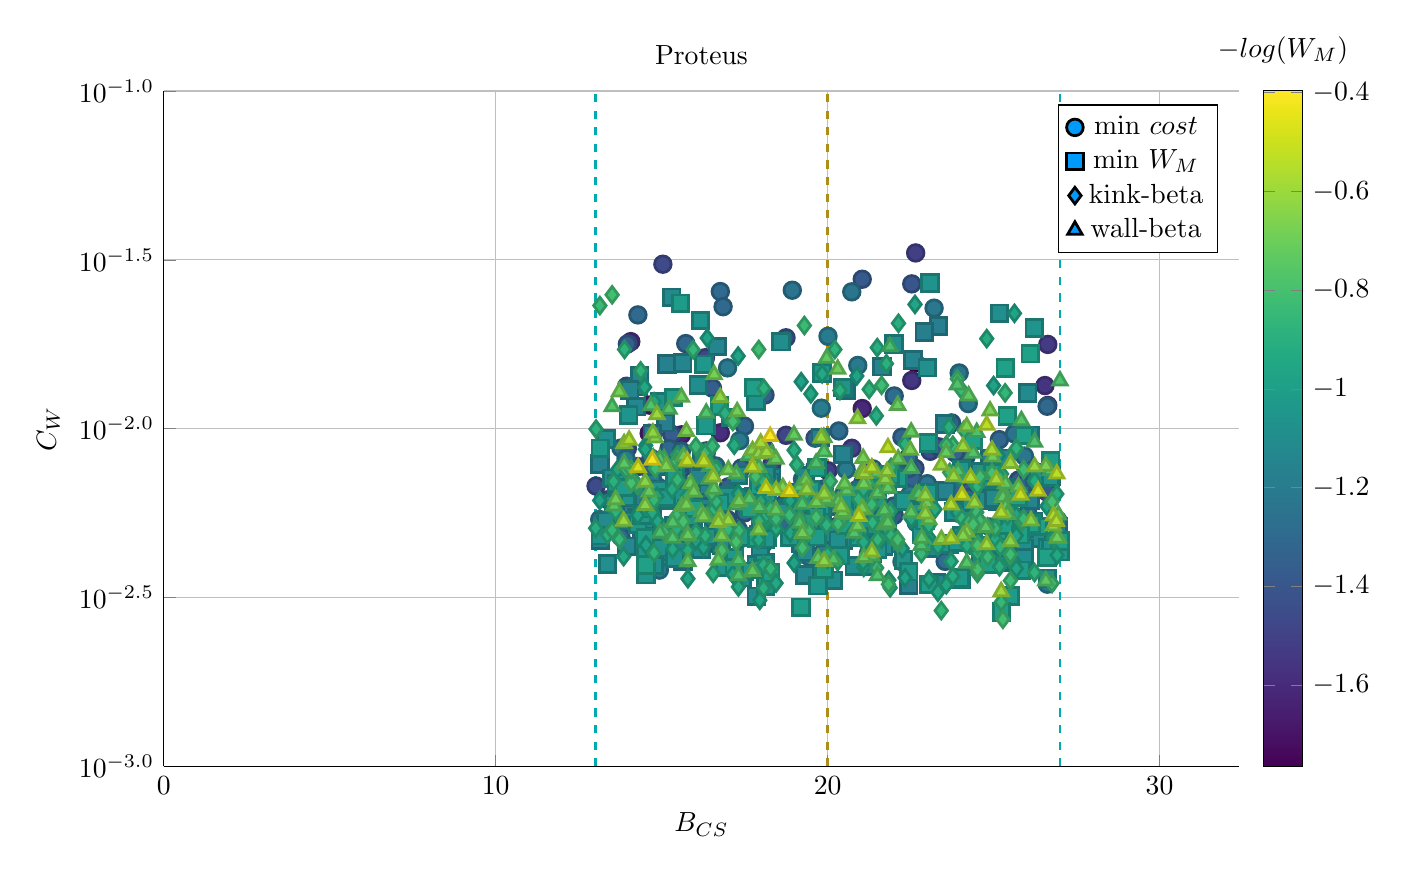
\begin{tikzpicture}[]
\begin{axis}[colorbar = {true}, height = {101.6mm}, ylabel = {${C}_{W}$}, title = {Proteus}, xmin = {0.0}, xmax = {32.398879571197455}, ymax = {0.1}, ymode = {log}, xlabel = {${B}_{CS}$}, {unbounded coords=jump, scaled x ticks = false, xticklabel style={rotate = 0}, xmajorgrids = true, xtick = {0.0,10.0,20.0,30.0}, xticklabels = {0,10,20,30}, xtick align = inside, axis lines* = left, scaled y ticks = false, yticklabel style={rotate = 0}, log basis y=10, ymajorgrids = true, ytick = {0.001,0.0031622776601683794,0.01,0.03162277660168379,0.1}, yticklabels = {$10^{-3.0}$,$10^{-2.5}$,$10^{-2.0}$,$10^{-1.5}$,$10^{-1.0}$}, ytick align = inside, axis lines* = left,     xshift = 0.0mm,
    yshift = 0.0mm,
    axis background/.style={fill={rgb,1:red,1.00000000;green,1.00000000;blue,1.00000000}}
, colormap={plots}{rgb=(0.26700400,0.00487400,0.32941500), rgb=(0.27794100,0.05632400,0.38119100), rgb=(0.28291000,0.10539300,0.42690200), rgb=(0.28229000,0.14591200,0.46151000), rgb=(0.27619400,0.19007400,0.49300100), rgb=(0.26514500,0.23295600,0.51659900), rgb=(0.25042500,0.27429000,0.53310300), rgb=(0.23360300,0.31382800,0.54391400), rgb=(0.21813000,0.34743200,0.55003800), rgb=(0.20123900,0.38367000,0.55429400), rgb=(0.18555600,0.41857000,0.55675300), rgb=(0.17117600,0.45253000,0.55796500), rgb=(0.15772900,0.48593200,0.55801300), rgb=(0.14618000,0.51541300,0.55682300), rgb=(0.13374300,0.54853500,0.55354100), rgb=(0.12346300,0.58168700,0.54744500), rgb=(0.11948300,0.61481700,0.53769200), rgb=(0.12632600,0.64410700,0.52531100), rgb=(0.15014800,0.67663100,0.50658900), rgb=(0.19109000,0.70836600,0.48228400), rgb=(0.24607000,0.73891000,0.45202400), rgb=(0.31192500,0.76782200,0.41558600), rgb=(0.37777900,0.79178100,0.37793900), rgb=(0.45867400,0.81636300,0.32972700), rgb=(0.54552400,0.83803900,0.27562600), rgb=(0.63690200,0.85654200,0.21662000), rgb=(0.73088900,0.87191600,0.15602900), rgb=(0.81457600,0.88339300,0.11034700), rgb=(0.90631100,0.89485500,0.09812500), rgb=(0.99324800,0.90615700,0.14393600)}, colorbar style={title=$-log( W_M )$}}, ymin = {0.001}, width = {152.4mm}]\addplot+[scatter, scatter src=explicit, only marks = {true}, color = {rgb,1:red,0.00000000;green,0.60560316;blue,0.97868012},
draw opacity=1,
line width=0,
solid,mark = *,
mark size = 3.0,
mark options = {
    color = {rgb,1:red,0.00000000;green,0.00000000;blue,0.00000000}, draw opacity = 1.0,
    fill = {rgb,1:red,0.00000000;green,0.60560316;blue,0.97868012}, fill opacity = 1,
    line width = 1,
    rotate = 0,
    solid
}] coordinates {
(22.651942134178245, 0.015650867313707448) [-1.7651507846396934]
(14.624587492471523, 0.009694646552347688) [-1.652530796858066]
(14.624587492471523, 0.011744038729478485) [-1.647000146345283]
(15.59515103457413, 0.009590177278586947) [-1.6184546481250472]
(21.041924335629172, 0.011474300333025303) [-1.6124908438767973]
(16.768060529085655, 0.00972401084478665) [-1.5828949402967583]
(14.070903864396604, 0.018106858351787505) [-1.577618500437912]
(26.63211955782928, 0.011719738653164523) [-1.56873554690934]
(26.54729756362062, 0.013419897432724169) [-1.5599002750009094]
(22.534449427914588, 0.013892471464509717) [-1.5518482038436605]
(26.63211955782928, 0.017767343192357253) [-1.5302287668791192]
(22.651942134178245, 0.033146306422516245) [-1.5115301730224102]
(20.011081752470886, 0.007510212646674021) [-1.5013825191439996]
(20.72766466016537, 0.008751202105526691) [-1.4958902811815062]
(15.146473848919625, 0.00816949735167802) [-1.4892617900728689]
(24.953221543185066, 0.008118078139228204) [-1.4884348201277007]
(18.74607790769805, 0.009559158760396884) [-1.4866425610729714]
(16.318569485171636, 0.01623184139531336) [-1.4835478223239928]
(18.31823242637104, 0.007837831837729894) [-1.4780728724015184]
(15.036815235314387, 0.03069401611625924) [-1.4650031348255397]
(13.023841119875671, 0.006765803188842749) [-1.4601242927308113]
(23.08827436791659, 0.008568870415676909) [-1.453691298071198]
(14.283963091120235, 0.007723927816166263) [-1.4489094778079963]
(13.382063426709323, 0.006162431971740805) [-1.432973868001932]
(18.11370115924847, 0.006329451983138475) [-1.4325147285303634]
(23.34059635854204, 0.008839617844718544) [-1.4268866569895065]
(13.967685136763796, 0.008744700190770928) [-1.4268347679685771]
(18.74607790769805, 0.018590297650719324) [-1.4237681445033143]
(16.531939570236105, 0.007587250291191641) [-1.4234658725845162]
(18.117461030315134, 0.007390656211515189) [-1.4109108269606008]
(18.117461030315134, 0.008694085637837138) [-1.4079262096010774]
(19.068604275965242, 0.00634066157530613) [-1.407330123320285]
(22.534449427914588, 0.026840973164111593) [-1.3996791570309395]
(25.747123007837175, 0.007040053838733538) [-1.3974870797438]
(13.944355842468203, 0.013359280479800206) [-1.3946269662443698]
(22.631885608490197, 0.007634837530984513) [-1.3905305073664083]
(26.612756674676874, 0.006488653571629467) [-1.3895960301339119]
(16.513096841535003, 0.00554611680879456) [-1.381931002288656]
(21.069685019437017, 0.00695131625200887) [-1.3818272949203658]
(21.041924335629172, 0.027704627448181397) [-1.3812563757949996]
(14.736556573901334, 0.00681167564679013) [-1.379699079550137]
(15.578926279356907, 0.006715817539753603) [-1.376650573885692]
(15.578926279356907, 0.00757067906104037) [-1.3758581110553065]
(24.170613812194496, 0.006499559071472007) [-1.375220700855124]
(23.73345635781125, 0.00646934556613389) [-1.3742348635950123]
(18.987744543833536, 0.0063267927368600325) [-1.3713423550361032]
(24.170613812194496, 0.008267480512087599) [-1.370057699317172]
(21.364079170448615, 0.004988896324536347) [-1.3686239973313072]
(22.006250519027304, 0.005540386026064644) [-1.3680076928767484]
(16.643751715736272, 0.005024205798518008) [-1.3672266212882762]
(15.300354897105095, 0.009628839399324697) [-1.3667105305870977]
(25.983749051053568, 0.0050592629231849704) [-1.3651176317240314]
(13.967685136763796, 0.017814080806893125) [-1.3612722200713383]
(15.565992883535738, 0.007840171434328094) [-1.360737823431438]
(16.531939570236105, 0.013182987051350502) [-1.3596008789905631]
(17.009377486662636, 0.006730765435871485) [-1.3568098625263256]
(17.49511712424178, 0.005632641769207446) [-1.3562925407270994]
(23.9635738853514, 0.005613911931897123) [-1.3540300242042478]
(20.336854083719853, 0.005176189759381431) [-1.3527684291391184]
(19.620614991884782, 0.007678792615766904) [-1.3513432280511455]
(25.983749051053568, 0.006888425944911811) [-1.3508742741062625]
(23.84218963638598, 0.006674090356682625) [-1.348444904526092]
(23.73345635781125, 0.010402669872398145) [-1.3482429808137002]
(19.620614991884782, 0.009376571407375644) [-1.3481015746033576]
(18.11370115924847, 0.012583797530216616) [-1.34746159692277]
(22.569231891000115, 0.007115527316776566) [-1.3450418873098828]
(24.492468867569784, 0.006464286011476574) [-1.3449397649071608]
(13.63676824165126, 0.006186516144095541) [-1.344834769873685]
(16.985654434835766, 0.0053864817732829605) [-1.3436955024234147]
(23.84218963638598, 0.00848434463520388) [-1.3426163725681677]
(15.156092946594729, 0.004938310227983135) [-1.3374912582230194]
(19.892081526120066, 0.006636608478826529) [-1.335539302100867]
(21.364079170448615, 0.007606581585076429) [-1.3352915983538123]
(14.277566761363651, 0.006029019944814239) [-1.331337874103357]
(16.34367742556589, 0.008594819258321628) [-1.3310780697195672]
(16.372753180241236, 0.004728216221281147) [-1.3292068036291638]
(18.651304149911, 0.005953363383436291) [-1.32828646244698]
(22.23750424468451, 0.009441137210103956) [-1.3280975618898123]
(14.816548429122673, 0.005079524630506098) [-1.3278697867431468]
(16.278758069854046, 0.005749625528658903) [-1.327757292865828]
(24.236502870832883, 0.006249734903697681) [-1.3253106415861637]
(21.376974447323292, 0.005155209960292018) [-1.3237407060184172]
(17.406035904117076, 0.007650804529712704) [-1.3217246458754282]
(16.676591700948407, 0.004926318213851794) [-1.319376268743699]
(20.218859975126456, 0.004774448071559269) [-1.3182101821558738]
(20.90842789138097, 0.0066268624262571275) [-1.31770129332637]
(15.726344083812931, 0.017867829271260238) [-1.3171626271127284]
(20.509174541398565, 0.006479743346210051) [-1.3144438328362922]
(17.49511712424178, 0.010177994071422254) [-1.314397397461996]
(25.17536025842546, 0.009279261565995508) [-1.3134452963620502]
(16.443823660899717, 0.005896178522672516) [-1.3126768401499638]
(21.376974447323292, 0.007223214696135702) [-1.3123916957087167]
(14.585638446869181, 0.007643344629724278) [-1.3117090270675453]
(14.29222630999366, 0.0062843154751196315) [-1.3112976001573549]
(19.34016378549167, 0.006316305209750007) [-1.3102933400586538]
(26.612756674676874, 0.011655743235665423) [-1.3084666426112759]
(14.677311567391737, 0.008181643780093392) [-1.3081739820914746]
(23.930583881480565, 0.005920113041607297) [-1.3081169022767745]
(18.59998810930447, 0.005266304291939928) [-1.3075986397555424]
(21.639804877968437, 0.0056632699287416785) [-1.3038897119548887]
(14.341073675298674, 0.004515583648974614) [-1.3034916079905217]
(22.44852739031052, 0.00762405310841983) [-1.301506470226052]
(14.283963091120235, 0.021723513711501174) [-1.2978787946122285]
(23.797921766937304, 0.005860560202229156) [-1.297460949292816]
(16.768060529085655, 0.02547444831481485) [-1.2953226778576867]
(16.850723243246257, 0.022974551007964673) [-1.2951062787178942]
(15.221638230176215, 0.008727794605170999) [-1.2946978796261759]
(21.194827607120533, 0.00606442154900928) [-1.293243062455323]
(13.773496878720852, 0.00478216163852665) [-1.2916316854649297]
(16.312384742623273, 0.004505685536187866) [-1.291573412415986]
(19.299286366301942, 0.006201757851874389) [-1.2910367642815292]
(14.715733335251208, 0.007056272547770033) [-1.2894268757747884]
(14.861104082210852, 0.004812007322004063) [-1.2891780169645117]
(21.99387616545991, 0.005900795309436559) [-1.2883016772579983]
(18.07568232599605, 0.004575860387174974) [-1.2877120777365891]
(16.5278219937302, 0.007501625869556503) [-1.2825608117529994]
(23.540570660663604, 0.004048206616482656) [-1.2803416949249293]
(22.006250519027304, 0.012501014524680899) [-1.2790944723531177]
(20.336854083719853, 0.009849033693022476) [-1.2789599032268324]
(21.229554500357366, 0.004266328381972482) [-1.278637308935949]
(14.019194247307421, 0.00602317781329061) [-1.2752962713941192]
(22.427243379042164, 0.008202673797589401) [-1.2724318730764337]
(19.80983944525114, 0.005313590913225172) [-1.26778944603233]
(15.630962235184002, 0.005746237915345085) [-1.2652894696394015]
(16.169659899199626, 0.0063394092295352205) [-1.263844406219344]
(19.370057307761773, 0.004670640784960837) [-1.2622412045786418]
(17.31176227830558, 0.005025369604276285) [-1.2622057750392766]
(17.350614255078973, 0.004715175023029078) [-1.2568407944078956]
(25.92926544649174, 0.005515822538041083) [-1.2564369672634057]
(13.773496878720852, 0.008763742702873716) [-1.255580803936347]
(19.24342166986986, 0.007090160917314494) [-1.2542825781236586]
(25.62853126166569, 0.009658252430988482) [-1.253606675738751]
(16.629549912781222, 0.005078101074449218) [-1.2533258835374417]
(21.331324879071882, 0.004668333949768413) [-1.252740293490489]
(26.02926384975561, 0.005623439530060779) [-1.2512906609771755]
(21.229554500357366, 0.007192663750971734) [-1.2505906665339703]
(26.93045024335227, 0.004753912504004936) [-1.2505667349102745]
(21.770706681119528, 0.00547669175115548) [-1.2505409706978425]
(15.59515103457413, 0.008585550973626429) [-1.2504311283223648]
(26.93045024335227, 0.00536142422310656) [-1.2495193060816674]
(22.748668314502247, 0.005891517799670805) [-1.2472203996667584]
(18.935691126914783, 0.025703839631456088) [-1.246340221801285]
(25.42163009914487, 0.004426672964739238) [-1.246337044553182]
(20.46656298748178, 0.004733745531528537) [-1.2444533586241864]
(19.245483292983383, 0.004373459187272198) [-1.2410504069560844]
(23.9635738853514, 0.014622918962551527) [-1.2404616678069278]
(20.72766466016537, 0.025422666134658947) [-1.2402101811954278]
(26.22602836680247, 0.00699405114862055) [-1.2399625556579728]
(19.15392842040434, 0.005459593535350185) [-1.2395775558220574]
(16.17194115370324, 0.006780135026174841) [-1.238968027160994]
(14.289259863079467, 0.006381273355008305) [-1.2381935518916032]
(19.245483292983383, 0.005454977773134567) [-1.2372164242860222]
(14.084051213081182, 0.006162937475975255) [-1.2359322527835273]
(25.92926544649174, 0.008295248979234676) [-1.2345953253761524]
(13.882021490725897, 0.005661235915534237) [-1.2333782101635051]
(24.89028576683355, 0.005116145429327062) [-1.2329256482335589]
(23.00100122686372, 0.0068738253515159406) [-1.2318041138227]
(16.629549912781222, 0.007759607253139788) [-1.2286780396839752]
(19.836396597287973, 0.004270512991179436) [-1.225800447150557]
(23.207115019583632, 0.022744869820021597) [-1.2237626122718148]
(17.350614255078973, 0.009221148903357415) [-1.2192315569877235]
(24.236502870832883, 0.011868028475244749) [-1.2191811590789894]
(16.34367742556589, 0.008481483201532794) [-1.2185680785343938]
(15.115258956268827, 0.00622802822970762) [-1.2179132583990178]
(14.90981948109104, 0.006703260233628488) [-1.2171472173843672]
(14.749136049291781, 0.00633213628058925) [-1.2167448502658762]
(20.90842789138097, 0.015392818825938645) [-1.2162995250149307]
(17.846164384152665, 0.003872910530196867) [-1.215703789534109]
(20.52604477006502, 0.004720977485089404) [-1.2156312790675603]
(22.124486957585535, 0.00736963569440644) [-1.2145283350978044]
(13.134678555839974, 0.005383150867826381) [-1.214317974252912]
(19.4366251326122, 0.004178935326843822) [-1.2138536176262873]
(26.62064413932083, 0.0034641548226198885) [-1.2119360055173332]
(14.931149108977916, 0.0038140534914709043) [-1.2104347246988538]
(20.557603047451465, 0.007570292211977012) [-1.2084631186053005]
(19.77593528714308, 0.0052385995930077645) [-1.2083264519217767]
(19.161909349795547, 0.005083028024589718) [-1.2073346872626274]
(22.23981527386949, 0.004039129704078142) [-1.2071975929322125]
(16.985654434835766, 0.01513911751066285) [-1.2067840670536927]
(22.486042313795984, 0.006395373245847939) [-1.206736577191552]
(26.236300999552455, 0.007483645463069493) [-1.2065799786199445]
(13.956526564952654, 0.005698374888186277) [-1.203843641047789]
(21.81360757918857, 0.005550896360654382) [-1.203724365314369]
(20.463153166774777, 0.005010777712400389) [-1.2024406864855146]
(14.715733335251208, 0.007157947201399507) [-1.2021169810907544]
(20.011081752470886, 0.01877759730610099) [-1.2015933815507112]
(14.00713301228089, 0.004489267037355289) [-1.2014423796656961]
(13.92658713143997, 0.006374667856956503) [-1.2011965112492808]
(14.486497670639796, 0.00572395742880883) [-1.2005427289121806]
(14.736556573901334, 0.0066192080125215165) [-1.1994215784439877]
(22.133490212694397, 0.007316062816603203) [-1.1975084180232178]
(19.80983944525114, 0.011502671870448664) [-1.1972619972446426]
(22.67137053609239, 0.005266662336518346) [-1.1967371969067386]
(26.735167824179122, 0.004368135902166705) [-1.1965134818457024]
(13.92658713143997, 0.008154332104698897) [-1.196084536648355]
(15.58476565413219, 0.006843978332329513) [-1.1943424204563022]
(25.30217158353333, 0.005029914775543452) [-1.1908054127888088]
};
\addlegendentry{min $cost$}
\addlegendentry{min $W_M$}
\addlegendentry{kink-beta}
\addlegendentry{wall-beta}
\addplot+[scatter, scatter src=explicit, only marks = {true}, color = {rgb,1:red,0.00000000;green,0.60560316;blue,0.97868012},
draw opacity=1,
line width=0,
solid,mark = square*,
mark size = 3.0,
mark options = {
    color = {rgb,1:red,0.00000000;green,0.00000000;blue,0.00000000}, draw opacity = 1.0,
    fill = {rgb,1:red,0.00000000;green,0.60560316;blue,0.97868012}, fill opacity = 1,
    line width = 1,
    rotate = 0,
    solid
}] coordinates {
(15.115258956268827, 0.010422279639263054) [-1.1890033537880158]
(14.715733335251208, 0.009658294464102987) [-1.1883675827161198]
(14.289259863079467, 0.013313745665171912) [-1.1879538738656286]
(19.892081526120066, 0.006487414571263668) [-1.1878029685724296]
(23.34059635854204, 0.020145877705477357) [-1.186260879134981]
(16.751068465480447, 0.005801884747670386) [-1.1859242026174677]
(20.313030948006798, 0.004217349677698315) [-1.183889066210908]
(20.08100946018568, 0.0058827996938258294) [-1.1830291222504283]
(24.89028576683355, 0.008160599297710009) [-1.1826268505607591]
(14.406348579120323, 0.004857174007518612) [-1.182365307189366]
(22.908762374221453, 0.01935279381255584) [-1.1822251925764147]
(20.278362500869783, 0.00447855648592392) [-1.1813612663460882]
(21.35046825241222, 0.00428725320402622) [-1.1785285195809967]
(15.6446694279654, 0.004053651772674214) [-1.1775655951090325]
(26.95198308809553, 0.005121496915389368) [-1.17705398157876]
(14.277566761363651, 0.005890819973806921) [-1.1767452937515073]
(25.12415251137596, 0.006104718148251412) [-1.1766083315756861]
(15.156092946594729, 0.01556268699280997) [-1.173888237216638]
(16.269054087414798, 0.005882961839613334) [-1.1734465174435744]
(20.278362500869783, 0.005961179911412564) [-1.1729466514857931]
(14.227206890976186, 0.006287276174883399) [-1.172839252676928]
(14.119035956708807, 0.005599267038542826) [-1.1727769211527406]
(26.11020939532839, 0.005070632392189801) [-1.1727372361954858]
(22.439521795398957, 0.003434292526080427) [-1.1726542785062386]
(17.248393366297435, 0.0062657093568900535) [-1.1703764252048678]
(16.5796794571122, 0.004942047034638912) [-1.1699166462753263]
(17.970910867302806, 0.004183590560340062) [-1.1681831393061217]
(16.624697426657203, 0.005170881199231806) [-1.1671080842733117]
(16.379855484535224, 0.006777996547666784) [-1.1655606692177785]
(20.463153166774777, 0.008402469668507205) [-1.165303541813206]
(13.151972673873539, 0.004666935296152095) [-1.1643973078802388]
(20.460136716993496, 0.004663766235492665) [-1.1632535008384055]
(19.2031189942159, 0.004566940606242733) [-1.1631989573193973]
(19.83550100861325, 0.0054331000812183365) [-1.1630392685982025]
(23.569327548205543, 0.006544368204474158) [-1.1625753891662707]
(13.671384109436172, 0.006511116933487475) [-1.1617936783337066]
(22.51827341524219, 0.006126048639979384) [-1.159367616011031]
(20.557603047451465, 0.012995381528200805) [-1.1593260324319568]
(18.135261940423753, 0.004013416769217783) [-1.1592024857112633]
(15.652603562708304, 0.004530529794416821) [-1.1590403977294572]
(13.139446789187307, 0.007867971330715704) [-1.1589428109110296]
(16.76328611632, 0.005330271588661515) [-1.158451320077056]
(14.857639167188884, 0.007724720119696045) [-1.157468772898154]
(24.758718787792066, 0.004436262085616985) [-1.1570637161067505]
(16.10076446545596, 0.007249642226094706) [-1.1563966451418943]
(19.77593528714308, 0.009420901412013665) [-1.1561531921827275]
(24.04992975868823, 0.0057898611640113395) [-1.1538328200442942]
(26.735167824179122, 0.007237376261288284) [-1.1525173430901554]
(17.092107947023983, 0.004881019954742076) [-1.1522162283529644]
(17.644214712877762, 0.0059379940430840635) [-1.151968932860403]
(26.108450807284747, 0.0061407721476487214) [-1.1511586507355254]
(21.639804877968437, 0.015255960449664327) [-1.1509834966159156]
(23.06727295287375, 0.004419080970160178) [-1.1503660387736743]
(23.540570660663604, 0.01032617135589161) [-1.1500086948877408]
(25.200810274108626, 0.004014883666259908) [-1.1494080253790357]
(19.32885457468507, 0.005291422749753008) [-1.1493093072503229]
(22.569231891000115, 0.01598351560152435) [-1.1489823622220707]
(21.074369777477393, 0.003915099463846501) [-1.1484511044037433]
(25.27069929453632, 0.005020529922825154) [-1.1483999797493492]
(23.27207804604334, 0.0034947010100993764) [-1.147064765638366]
(14.719150012234948, 0.005859550653426385) [-1.1465028274549764]
(24.247203750488318, 0.005641165149475234) [-1.144883586902141]
(18.31823242637104, 0.007176119328254024) [-1.144368544047569]
(16.20920986207578, 0.00802165691682325) [-1.1435280806157744]
(14.246324004196616, 0.005447269817044685) [-1.1433393449411435]
(25.35315185019304, 0.006668732693209443) [-1.143332108158641]
(19.971681515811508, 0.004886014774808058) [-1.143184585873657]
(16.676591700948407, 0.017515494611674454) [-1.1428249654095861]
(14.341073675298674, 0.014377117697389604) [-1.1427984862828113]
(14.040817864118065, 0.013005276311642224) [-1.142397010267489]
(21.194827607120533, 0.005929095379259443) [-1.1423708774410877]
(15.630962235184002, 0.01565086593371781) [-1.1422424769576425]
(19.32885457468507, 0.007266091038483963) [-1.140012696356206]
(20.5792220239773, 0.005840600330748377) [-1.1399465227440013]
(25.415403683525007, 0.00480284773560221) [-1.1387943392990294]
(19.654837660739332, 0.005752426766742318) [-1.1382802201938975]
(14.227206890976186, 0.011612930840038163) [-1.1380314198362265]
(19.150893512430507, 0.006446360072583165) [-1.137892443914052]
(26.11020939532839, 0.009562541252399106) [-1.1311113631375915]
(20.922532876081345, 0.005743536904522906) [-1.1302954325651586]
(24.59831707555059, 0.0041760314888273755) [-1.1295543261638465]
(14.802199219727623, 0.006161648966500728) [-1.129462828049983]
(19.31280667855182, 0.00369116854025651) [-1.1277963061708562]
(21.467959067562802, 0.006278926396423389) [-1.126807171194116]
(13.95165441994897, 0.004487529275565533) [-1.1267021554022474]
(18.269334848839954, 0.006938744439971839) [-1.1265761162904897]
(19.31280667855182, 0.004304336836767321) [-1.1261385034152473]
(15.968611966724305, 0.005917258047258142) [-1.1260458936236624]
(18.85019132037221, 0.005885263457738176) [-1.1250537668582923]
(14.486497670639796, 0.005616858230043609) [-1.124511019242948]
(17.9238683493206, 0.004843731890681865) [-1.1236988869720232]
(25.85696228036533, 0.005173923137495115) [-1.1235064786985465]
(19.860778911496865, 0.003624821435760545) [-1.1232730371267585]
(18.135261940423753, 0.007429853985811719) [-1.1231293548483412]
(14.36713722146902, 0.005231942783984398) [-1.1209978185544383]
(25.27069929453632, 0.008169617815892689) [-1.1196911148335087]
(24.792905974230315, 0.0061580609115664325) [-1.1194748634113345]
(14.94576539459215, 0.004188882178419093) [-1.119418152841014]
(17.83202655689412, 0.005791769416647159) [-1.1191123923650526]
(21.037434506959272, 0.004931972266091366) [-1.1181736482095217]
(16.33802128070243, 0.005611347227289511) [-1.1176702646643628]
(15.300354897105095, 0.024480989089009208) [-1.1175403888423328]
(16.804752354132532, 0.004518885765871233) [-1.1174827013795072]
(24.9997310960539, 0.0062233325455323925) [-1.1174414411464733]
(13.95165441994897, 0.006299808378708293) [-1.1171134960728113]
(21.91021863095728, 0.004568184715721437) [-1.1171111976535804]
(26.02926384975561, 0.012757776435747556) [-1.1168806186241906]
(18.159403641727735, 0.007305420869085463) [-1.1160945644374545]
(13.321210613736467, 0.005340773800773009) [-1.1139896885893594]
(17.421485223983048, 0.0036233885329560954) [-1.1123768792739945]
(26.198956758292148, 0.005311493039288053) [-1.1112153482766423]
(21.686800668420936, 0.0045000578497955725) [-1.1111283014916062]
(17.850925724336616, 0.003188662256079057) [-1.1108869662710774]
(19.233603569785046, 0.004842654136629077) [-1.1089922492653659]
(25.347291504394295, 0.00452032863173795) [-1.108391782497311]
(14.504420816138161, 0.00535669926333167) [-1.1082929384878708]
(26.32188665435516, 0.004745534590751309) [-1.1074346113685616]
(17.970910867302806, 0.004323464728471098) [-1.1074227437950106]
(17.30594937629188, 0.007293078759243216) [-1.1069130893453907]
(17.850925724336616, 0.003945456212149148) [-1.106325178133445]
(21.792402805381546, 0.004982808461571556) [-1.1060035644106432]
(17.970910867302806, 0.0052409052861536465) [-1.1038776732161713]
(21.069685019437017, 0.0065314531396132094) [-1.10351060592976]
(15.354808162096106, 0.005173060010686301) [-1.1022315889718237]
(17.92907707816459, 0.005951424789746293) [-1.1016702257969113]
(24.59831707555059, 0.007437806150470808) [-1.100448826904311]
(15.948854285961046, 0.005288339533793414) [-1.0998565094908217]
(14.961732146234509, 0.004337170224988449) [-1.0995498480529582]
(25.430993986088392, 0.005750254423520601) [-1.0992970719713648]
(25.92565373787029, 0.004423364554484401) [-1.0987351440216522]
(25.430993986088392, 0.006535275113176343) [-1.0983869460625248]
(21.792402805381546, 0.006822630998366228) [-1.0977261444257258]
(21.99387616545991, 0.017828562633364364) [-1.0969882385788774]
(16.191435661836504, 0.004407786879742766) [-1.096807077081938]
(25.920441712682297, 0.0041501216036249275) [-1.0962033310727437]
(13.367816836249185, 0.003972749736578854) [-1.0948458082881816]
(23.00100122686372, 0.015155543307471772) [-1.093965318294314]
(16.10076446545596, 0.013471957430229371) [-1.093275686079877]
(20.800547804595237, 0.003923510470624812) [-1.0931318196649105]
(18.59998810930447, 0.01811006730780237) [-1.0926393639694263]
(23.797921766937304, 0.005671433069083637) [-1.09199330517098]
(20.172158161026072, 0.0035546432563184145) [-1.0916603258728452]
(25.920441712682297, 0.005082501155756355) [-1.091508438458307]
(21.322964695317083, 0.003922207642532424) [-1.0911853630489914]
(13.508356065492707, 0.007129588907950501) [-1.0896526200520398]
(25.41312647977644, 0.004468466025444819) [-1.088663441639713]
(25.17536025842546, 0.021949864805969728) [-1.0877780715734315]
(13.321210613736467, 0.009322832924906896) [-1.0870739196827126]
(20.321218652713394, 0.004672088916974179) [-1.0855818982110972]
(17.197220657946232, 0.004039319528471343) [-1.0844715994400023]
(13.872957163284784, 0.0053439960085053) [-1.0842780595786392]
(22.748668314502247, 0.005760793758021615) [-1.084266572782003]
(21.108662110316036, 0.00569380985136289) [-1.0839928767281124]
(14.775761073278609, 0.0039349920083461085) [-1.0828594792618813]
(14.806549696522097, 0.0062405207423892875) [-1.082853352734588]
(18.145601806636947, 0.0054577800846403015) [-1.0824719035597]
(24.020772375357197, 0.0035809652689903063) [-1.0824709528228211]
(21.25065104433097, 0.005148297391297789) [-1.0814366033908964]
(15.662032516582798, 0.006582162000449632) [-1.0809878234039578]
(17.764718157329845, 0.006301853688415234) [-1.0808972954130593]
(17.421485223983048, 0.006161790226168522) [-1.0797863646031054]
(26.62064413932083, 0.0036086053477567665) [-1.079163153355685]
(16.368956330173987, 0.004793357206410555) [-1.0780309855478056]
(15.902251231898113, 0.0054298508521766365) [-1.076806285491668]
(19.34016378549167, 0.00604411217248383) [-1.0765985094568509]
(24.032420298396573, 0.004828662165485411) [-1.0760641298404754]
(18.651304149911, 0.005661819547798889) [-1.0757730303287785]
(26.62064413932083, 0.00443044659495794) [-1.0744056068515366]
(15.866386736192135, 0.005467468655559742) [-1.073726482715373]
(24.306579484746003, 0.006046667097602973) [-1.072815333291583]
(17.009377486662636, 0.006315687038558954) [-1.0718638391063322]
(14.931149108977916, 0.011989877345034696) [-1.0710072465261937]
(21.322964695317083, 0.006287200186056995) [-1.0706716976099708]
(26.32188665435516, 0.00739594343637032) [-1.069478881808043]
(17.846164384152665, 0.012080600310741674) [-1.0679830462657767]
(15.30993412600253, 0.006138341400017388) [-1.0670572282884458]
(22.284343035497017, 0.004085658341340117) [-1.0667391835901658]
(17.736283735115194, 0.006004004929014098) [-1.066302608545655]
(14.961732146234509, 0.004440975162005993) [-1.064104157833971]
(23.08827436791659, 0.026972932068461592) [-1.0640878812065675]
(21.508022779864863, 0.004395996587917252) [-1.0635820925869255]
(26.716640036139204, 0.004423420241739423) [-1.062988318250961]
(19.11527100708343, 0.00480727122317776) [-1.0628036997189863]
(18.131669417857122, 0.0034131330547271113) [-1.062700357913494]
(14.529712726466656, 0.0036974585830479817) [-1.0626514373993834]
(18.173944283111027, 0.004776499853086686) [-1.0610739421064752]
(15.401502456170876, 0.004144297606935685) [-1.0588352037418618]
(16.169659899199626, 0.0209014980088616) [-1.0585986545827941]
(14.00713301228089, 0.010988948677442597) [-1.057135771526312]
(20.46656298748178, 0.013241941603829825) [-1.056315661795303]
(26.22602836680247, 0.019862106250452566) [-1.0562734967702754]
(22.819346636869057, 0.004858658731965693) [-1.0561257856094448]
(19.11527100708343, 0.006223828461257365) [-1.0559814704124602]
(18.131669417857122, 0.004706089102701761) [-1.0555859489072712]
(18.079332919029085, 0.003994614402213268) [-1.0549803415205259]
(20.87914774430368, 0.006463993798881436) [-1.0545713902023608]
(16.908681604757444, 0.0038990516235787613) [-1.054205756099488]
(26.711777515939247, 0.007195479612398366) [-1.0536290024409787]
(13.929572546627387, 0.006286763322784177) [-1.0533216125601341]
(13.151972673873539, 0.004822724612666477) [-1.0529307720930816]
(22.819346636869057, 0.005656264568736301) [-1.0525850668019536]
(15.477350070944595, 0.006295530789348686) [-1.052552508886994]
(24.032420298396573, 0.007550888758433211) [-1.0509835312174363]
(15.45268981247694, 0.004904482654727138) [-1.0508250621973283]
(14.961732146234509, 0.006571304536184572) [-1.050680345054969]
(23.655268515644366, 0.004560195418506711) [-1.0506245233592775]
(17.092107947023983, 0.01080264515897382) [-1.0505217359121972]
(13.55338844221082, 0.00597835329976134) [-1.049317623712287]
(17.625908695494353, 0.00605275476812188) [-1.0490747591885061]
(24.537224497440306, 0.004511808104116367) [-1.0489907539423449]
(24.391233921325668, 0.0049153150140211965) [-1.0478434867034416]
(23.909126603799116, 0.004616652674773231) [-1.0473758850488442]
(18.173944283111027, 0.006447737760929581) [-1.046767629611379]
(22.284343035497017, 0.006114416229637186) [-1.0460742739305466]
(19.83550100861325, 0.01461141466329314) [-1.0428746875530057]
(19.710045895289856, 0.0034297894059699906) [-1.0409932776852704]
(26.99666218082735, 0.004324846597058025) [-1.040720375777512]
(13.63676824165126, 0.0068957525832947) [-1.0400494553390642]
(18.87182730714039, 0.0047742837106654985) [-1.03963800286999]
(24.953221543185066, 0.0070972253563865) [-1.0394862991533038]
(20.509174541398565, 0.006107051538135721) [-1.0391370640013136]
(16.278758069854046, 0.015503036624972183) [-1.038354289214968]
(23.035515049672192, 0.006445735380428859) [-1.0380750082543837]
(14.279438101093232, 0.005205902574339689) [-1.0370263081612092]
(21.737554950575895, 0.005283195240312258) [-1.0365321066837632]
(19.806577545472447, 0.005892181423629392) [-1.0364145571368009]
(16.33802128070243, 0.010214094301379546) [-1.0358730287795153]
(17.48698733172037, 0.003781581128188247) [-1.0352797650690977]
(21.495458720132525, 0.0061316127141858145) [-1.0352425491421158]
(14.518866161482416, 0.004345014451914255) [-1.0335536367675167]
(17.197220657946232, 0.00415632052734694) [-1.0319535365225938]
(15.134079464405815, 0.006253917955260214) [-1.031638330454266]
(23.993469701679754, 0.003613822408322808) [-1.0316283345953763]
(17.48698733172037, 0.00478160347928963) [-1.0312630056422283]
(24.747450186073678, 0.004326998549376461) [-1.030801418278412]
(16.751068465480447, 0.006039359373565179) [-1.0301227610636083]
(14.406348579120323, 0.005550817437725965) [-1.029015666765989]
(19.493426492317983, 0.006583295742064639) [-1.0288573869793878]
(20.37163275163815, 0.004204292638824563) [-1.0245024368116802]
(15.401502456170876, 0.007145400138218064) [-1.0231385619546913]
(19.68119459959854, 0.004789677204757558) [-1.021449027000752]
(17.924682632407837, 0.00675373673736514) [-1.0213127693885564]
(25.50482023490044, 0.003193542226257652) [-1.0209276741398987]
(22.124486957585535, 0.007121099635585821) [-1.0202684704954939]
(22.439521795398957, 0.0037708668397859442) [-1.0187837906200732]
(15.743591734002468, 0.005805595496214904) [-1.0179738483919518]
(23.035515049672192, 0.009070154520460257) [-1.0169425110693646]
(15.5630871969197, 0.00501503870041615) [-1.0162045101447212]
(13.869405436882781, 0.00670010251636303) [-1.0149810946438107]
(13.151972673873539, 0.008752580219573484) [-1.014353466976016]
(15.565992883535738, 0.023528952793841592) [-1.0140528730661398]
(19.665351838058136, 0.005527004085356763) [-1.0133093427968076]
(20.943775733817652, 0.004778958682375364) [-1.0128360857902137]
(18.033648098721542, 0.003842216867194081) [-1.0126834015105255]
(21.878860060352352, 0.007300503854095673) [-1.0124869131348806]
(25.83788180341901, 0.0038089628255598917) [-1.0084966915198963]
(26.716640036139204, 0.008048423371546378) [-1.005776006726422]
(26.339525393761082, 0.005136336479510988) [-1.0027757315503723]
(19.193829077288807, 0.0029594317443149176) [-1.002422823826331]
(23.0540274641531, 0.003459304695059543) [-1.0023352556688647]
(25.143925437510074, 0.004988217345842403) [-0.9994656987080655]
(26.999066309331212, 0.004649343635980374) [-0.9991953302395459]
(24.969602727169466, 0.007411548557741582) [-0.9991876183275935]
(17.18725041495652, 0.0038831217844692545) [-0.9971256954762724]
(25.239953702493796, 0.0028654321699102935) [-0.9968293366364798]
(24.38577334322156, 0.004992975570566671) [-0.9965130838642419]
(19.895557019888, 0.003830578946172306) [-0.9960911988132904]
(17.764718157329845, 0.013215773066776348) [-0.9953080727443692]
(22.937595078654155, 0.005338097758519931) [-0.994764309342816]
(14.62322740320338, 0.005798704578553127) [-0.9941918143808477]
(19.68119459959854, 0.007661762309327555) [-0.9939974184414383]
(15.354808162096106, 0.012372283627325148) [-0.9936895922796631]
(14.509582689075785, 0.0047417231470052315) [-0.9920762514365737]
(25.357682218729416, 0.005175409039233765) [-0.9891335090238219]
(17.644214712877762, 0.005799134035216279) [-0.988320863141931]
(24.822975077806525, 0.003975692742134705) [-0.9873980470532571]
(15.968611966724305, 0.005803966541873779) [-0.9872638091155089]
(19.372259092318934, 0.005281651647264406) [-0.9871243344745786]
(25.92565373787029, 0.00954881671016918) [-0.9862026242600886]
(24.391233921325668, 0.009231911938640338) [-0.9851939256634008]
(26.125739860092395, 0.005233428706224578) [-0.9845137991026185]
(25.35315185019304, 0.015110407509335635) [-0.9844063088607684]
(25.747123007837175, 0.006274740712107015) [-0.9843851675543582]
(26.108450807284747, 0.01666579340898781) [-0.9832677624207663]
(17.860630065422363, 0.004743145828135927) [-0.9823156156623659]
(18.28268228926236, 0.003744148435661381) [-0.9817957805945331]
(25.812435546384016, 0.0048552692105239565) [-0.9817262777133879]
(16.751068465480447, 0.01167873981501713) [-0.980944500204026]
(26.605009277171177, 0.004161496814710868) [-0.9808435285359967]
(25.41312647977644, 0.010903168023481107) [-0.9803069086017846]
(20.536092995679923, 0.005187973951951495) [-0.979926239566149]
(14.529712726466656, 0.0039527765780552285) [-0.9799255860420428]
};
\addlegendentry{min $cost$}
\addlegendentry{min $W_M$}
\addlegendentry{kink-beta}
\addlegendentry{wall-beta}
\addplot+[scatter, scatter src=explicit, only marks = {true}, color = {rgb,1:red,0.00000000;green,0.60560316;blue,0.97868012},
draw opacity=1,
line width=0,
solid,mark = diamond*,
mark size = 3.0,
mark options = {
    color = {rgb,1:red,0.00000000;green,0.00000000;blue,0.00000000}, draw opacity = 1.0,
    fill = {rgb,1:red,0.00000000;green,0.60560316;blue,0.97868012}, fill opacity = 1,
    line width = 1,
    rotate = 0,
    solid
}] coordinates {
(21.711893029131566, 0.0049343734079309275) [-0.9797193514246809]
(20.87914774430368, 0.014326928101993836) [-0.9793649258547107]
(22.249101100040285, 0.004418560150536774) [-0.9793554194238832]
(23.993469701679754, 0.007133046942930264) [-0.9793399260652301]
(14.529712726466656, 0.004527202123528333) [-0.9786718824413932]
(19.2031189942159, 0.013777079521683793) [-0.9784247640598123]
(25.079354543031585, 0.005278344797288595) [-0.9784156054323705]
(18.989026003231032, 0.004002965553163199) [-0.9772101816150688]
(24.9997310960539, 0.013418113026562503) [-0.9771245449599791]
(25.62847037709553, 0.004027289040267911) [-0.9768013676267739]
(16.372753180241236, 0.018551171796247393) [-0.9763993914483391]
(13.134678555839974, 0.006130885121857039) [-0.9762949474128021]
(16.427208297726143, 0.005562603331167774) [-0.9759999361809304]
(25.143925437510074, 0.008328856003390762) [-0.9748577786630778]
(19.99680496969866, 0.004109700372311695) [-0.9738966318394574]
(13.56697824167195, 0.004913914166672265) [-0.9734793512186626]
(16.03107337465876, 0.004665122126804512) [-0.9731032751395803]
(18.033648098721542, 0.006640697404806304) [-0.9726016535105552]
(24.427094392002633, 0.004736078134325021) [-0.9724572780741577]
(23.908352016960492, 0.005647304198937851) [-0.9722087723669882]
(24.79132961055872, 0.004389286248628818) [-0.9718244022964762]
(22.332295899617375, 0.0036192646662402627) [-0.970582002945255]
(13.671384109436172, 0.007574170243236733) [-0.9693863160362324]
(17.30594937629188, 0.016406094197261946) [-0.968978562403945]
(18.87182730714039, 0.004910644527520683) [-0.9682987091511867]
(21.62636840883897, 0.004713875842941002) [-0.9661896439247507]
(19.193829077288807, 0.005899389733384474) [-0.96458538139874]
(21.793166599979934, 0.0056286885015633895) [-0.9644132418595727]
(16.260430864278227, 0.004458328702018249) [-0.9642494738631832]
(26.605009277171177, 0.005896947846453336) [-0.9638749980488863]
(14.518866161482416, 0.008919099387898428) [-0.9633607889353855]
(17.144948028029052, 0.003704995647544644) [-0.9628913890413714]
(18.87182730714039, 0.00612171997200749) [-0.9627420883815555]
(21.843108678301228, 0.003560196433315863) [-0.9623524414535783]
(25.62853126166569, 0.02195538724653361) [-0.9620751879990892]
(17.955918213319755, 0.0031037314795763953) [-0.9616273380898692]
(23.06727295287375, 0.004737846584498155) [-0.9614728013262]
(22.9924640163578, 0.0056288454988440186) [-0.9611621976310423]
(17.31176227830558, 0.006420794710655912) [-0.9607076853432408]
(25.68282437564652, 0.004827398822111102) [-0.9600064809118957]
(22.631885608490197, 0.02333271298987377) [-0.9582788764682687]
(25.68282437564652, 0.005548252171458194) [-0.9582126253448857]
(23.06727295287375, 0.005664193052715976) [-0.9580357625022031]
(14.279438101093232, 0.005536719771654066) [-0.957784719926681]
(25.68559192901304, 0.003853864382102105) [-0.9569481934101607]
(16.556270886342375, 0.005755412847229535) [-0.9553125817248839]
(14.509582689075785, 0.008689466677368552) [-0.9542931196842905]
(16.58107133568487, 0.0059335279307082415) [-0.9535689234008579]
(22.517026888269854, 0.00540418577910244) [-0.9533577705177119]
(20.77275422833572, 0.004951751523060612) [-0.9524896594035642]
(15.790739414166003, 0.0035965091424978767) [-0.9519498604980341]
(16.804752354132532, 0.005225320910765454) [-0.9518141933322811]
(21.467959067562802, 0.0064487141747247515) [-0.9516817791582881]
(26.80433260075194, 0.004824944888873151) [-0.9503280372896984]
(24.08056889459325, 0.00494548994415281) [-0.9501901690400224]
(14.861104082210852, 0.005348280279251544) [-0.9501200807106565]
(23.575238252030694, 0.003451161099821506) [-0.9494094470373718]
(19.493426492317983, 0.012679296138241048) [-0.9485432404545778]
(14.861104082210852, 0.006306624155522614) [-0.9476409244484506]
(14.486497670639796, 0.013277570668597095) [-0.945668217439486]
(14.775761073278609, 0.012011087422302516) [-0.9455646191283261]
(26.913506127016916, 0.0042225651663969944) [-0.9452539976263535]
(21.817575837477094, 0.007400046119087899) [-0.9445379968061569]
(21.088494147417737, 0.0038853521635503845) [-0.9442842771351952]
(23.0540274641531, 0.003581425300578328) [-0.9439633256599537]
(19.836396597287973, 0.014533706969027229) [-0.9435190061725043]
(21.495170330924516, 0.005251128867230356) [-0.9431579759120018]
(23.32241055960176, 0.0032803092315458883) [-0.9428483368499935]
(16.76328611632, 0.005138967929828396) [-0.9422331530579936]
(18.447686620108747, 0.0034905159514662587) [-0.9396609276523904]
(21.074369777477393, 0.004029446318551389) [-0.939623008122614]
(23.0540274641531, 0.00455015926208741) [-0.9389137302612279]
(15.33021544852462, 0.00439803335731196) [-0.938282475354221]
(18.159403641727735, 0.007076676002554203) [-0.9381610470878076]
(13.855662151001413, 0.004180164094848145) [-0.9375089447207223]
(25.047879452913545, 0.0047224227678250175) [-0.9369328543779993]
(17.98391484948191, 0.0060949751266714085) [-0.9362670591806482]
(14.719150012234948, 0.005648330019282998) [-0.9352069487820426]
(24.387769811025546, 0.005000154489324483) [-0.9348472459577944]
(17.955918213319755, 0.005297957377087851) [-0.9342522553820941]
(21.495170330924516, 0.006759629185969791) [-0.9338432220939059]
(15.30993412600253, 0.006608248212098614) [-0.9331696663167082]
(23.32241055960176, 0.004476157560195598) [-0.9323821674335669]
(22.834131439170747, 0.004553679627799357) [-0.9312147370194936]
(24.537224497440306, 0.004658130964295737) [-0.930280167995953]
(18.447686620108747, 0.005060711761627857) [-0.9280045677807334]
(24.792905974230315, 0.018476285473848813) [-0.9280031254185547]
(17.312868144499753, 0.0034004941489706427) [-0.9276368843131759]
(24.59404027903679, 0.005166624841841688) [-0.9268239261037757]
(15.785946454503529, 0.004359745755123362) [-0.926124917347277]
(23.23495821442244, 0.005775582114052551) [-0.9257073204007308]
(17.18725041495652, 0.008935057639573897) [-0.924623493423007]
(19.158825560243013, 0.005284834073095107) [-0.9243237059537647]
(24.387769811025546, 0.006960808141066332) [-0.9233834598837832]
(24.764249505652145, 0.004477816754705252) [-0.9228152651263011]
(15.610110935591706, 0.005256266572834143) [-0.9225398322566478]
(21.086014975073198, 0.004614605578452094) [-0.9221817845745035]
(17.9238683493206, 0.004684328138894626) [-0.9215264386089611]
(13.011374727983977, 0.005073667236310502) [-0.9182360577808578]
(26.236300999552455, 0.00699448652183368) [-0.9171606639000199]
(25.496539583465434, 0.004096269252840535) [-0.9167994991962954]
(24.105981493227365, 0.004877105036737716) [-0.9148199077007076]
(18.145601806636947, 0.005333658362398189) [-0.9143950266851926]
(15.772215710533262, 0.0063326000908344015) [-0.9137204603649657]
(23.77209082045688, 0.003656199076187517) [-0.9133127453951064]
(26.905013263566943, 0.006406059775809559) [-0.9121627392578615]
(21.843108678301228, 0.006847766811629225) [-0.9120709030515949]
(21.074369777477393, 0.006587871594639965) [-0.9120475096142877]
(24.537224497440306, 0.006957117514637042) [-0.9120417957644669]
(21.88346447009828, 0.003379934383470047) [-0.9119544487627024]
(21.467959067562802, 0.010913194864582846) [-0.911708891151293]
(20.30332931675502, 0.004041226194685478) [-0.9111798161472054]
(25.239953702493796, 0.0073486956507704685) [-0.9107411837742436]
(26.79882485524314, 0.004735506056694406) [-0.9100560207797687]
(23.655268515644366, 0.010112207946458425) [-0.9096645202732524]
(18.989026003231032, 0.008635225183072814) [-0.9087883894803973]
(21.686800668420936, 0.005403661462545021) [-0.9082790009204854]
(23.71920555338414, 0.004047054134608013) [-0.9081431792626627]
(25.17696423356227, 0.003902974011235298) [-0.9067699437470415]
(21.495458720132525, 0.017382642208156447) [-0.9060971962820227]
(24.194837362132866, 0.004507017121233361) [-0.9060048430542386]
(18.442422810906905, 0.0054677225459759575) [-0.9051444524245076]
(19.99680496969866, 0.004250447610661418) [-0.9046954309394458]
(25.42163009914487, 0.005523706134151735) [-0.9046460109599029]
(15.469368499099941, 0.005058679669540388) [-0.9046042329773717]
(19.15808110804699, 0.004880341290688154) [-0.9039977279126346]
(13.367816836249185, 0.004848014991264962) [-0.9034337968845987]
(18.072238642477593, 0.0033710581928259836) [-0.9031566859943262]
(22.133490212694397, 0.02051608060889296) [-0.9023267465363606]
(18.072238642477593, 0.00394866132787808) [-0.9008355008980751]
(16.908681604757444, 0.011116102682336754) [-0.9007285357561787]
(16.552565712961382, 0.0037301270643077876) [-0.8972742280672815]
(13.55338844221082, 0.006975150409970039) [-0.897175036870542]
(24.511261732188537, 0.004282665596744035) [-0.8971186814881362]
(20.37163275163815, 0.012972814791692319) [-0.8969796612342156]
(23.05056195453426, 0.0051618357133361315) [-0.89672282177903]
(21.770706681119528, 0.015575744813995764) [-0.8963952627105445]
(18.269334848839954, 0.006658522954563811) [-0.8958485488547734]
(18.07568232599605, 0.005404120857058153) [-0.8943684288096996]
(22.332295899617375, 0.009007603010797853) [-0.8914082601651864]
(18.07568232599605, 0.006944169371814818) [-0.8896483571913044]
(19.99680496969866, 0.006491642132230442) [-0.8869865112217631]
(13.023841119875671, 0.009974107942199384) [-0.8866075677924622]
(18.079332919029085, 0.013162396177814029) [-0.8851823316418669]
(21.91021863095728, 0.004826124490303322) [-0.8846740900795415]
(13.616480154545364, 0.005684202227253982) [-0.8840192815000373]
(16.312384742623273, 0.0048201007942522064) [-0.8839767416908659]
(19.068604275965242, 0.007830361841197038) [-0.8835453569153728]
(19.968999576205356, 0.005186138093663713) [-0.8832514898254401]
(17.93627510472957, 0.0053254692875210185) [-0.8832295476215102]
(25.62847037709553, 0.008573190683116311) [-0.883069564455261]
(25.200810274108626, 0.004462559243137306) [-0.8830632191913902]
(21.88346447009828, 0.005696949886972815) [-0.8825797897872378]
(13.882021490725897, 0.01716789737474233) [-0.8801231316414504]
(21.35046825241222, 0.005269633409728344) [-0.8791867595932125]
(20.922532876081345, 0.006190708259408953) [-0.877951083604425]
(21.25065104433097, 0.013073202281995273) [-0.8774262288873376]
(15.902251231898113, 0.006886241915548495) [-0.8751523935645794]
(26.232326861807465, 0.003750268079957199) [-0.8748921304141444]
(14.36713722146902, 0.014828542032509849) [-0.874690516784764]
(14.771138015954458, 0.004289107281658671) [-0.8742887892359985]
(16.58107133568487, 0.005786133363621624) [-0.8739921539442262]
(25.68559192901304, 0.008747322528766296) [-0.8716524887679293]
(20.218859975126456, 0.01715728174165555) [-0.8712831508374237]
(15.469368499099941, 0.008344053133431154) [-0.8707782727491976]
(24.511261732188537, 0.006756312980238707) [-0.8688158783682262]
(17.009893524049446, 0.005033506475358252) [-0.8686482360373176]
(16.643751715736272, 0.0060832943243140855) [-0.8685858440662988]
(16.03107337465876, 0.004920623586218273) [-0.8672784286683882]
(19.370057307761773, 0.004866417685086465) [-0.866786932045215]
(25.17696423356227, 0.007171410952306857) [-0.8662743883953999]
(21.508022779864863, 0.004690311648627596) [-0.8651646039969739]
(16.643751715736272, 0.007587597698564831) [-0.8649542416484729]
(16.20920986207578, 0.008493030870048135) [-0.8638854242016366]
(21.91021863095728, 0.007681026757569149) [-0.8637850725340939]
(18.28268228926236, 0.00385351424497451) [-0.8621520373035888]
(24.04992975868823, 0.005420954062013184) [-0.8611949292176813]
(25.347291504394295, 0.012767830297498842) [-0.8597568594294163]
(23.423616029838065, 0.0028935280651521448) [-0.859303050958753]
(15.477350070944595, 0.007054888627501927) [-0.85891018749718]
(13.508455039987684, 0.005004853345841743) [-0.8586165859116928]
(24.105981493227365, 0.009908479871966714) [-0.8586114389950454]
(14.771138015954458, 0.006151478093055551) [-0.8583221454358831]
(19.370057307761773, 0.006469455145345583) [-0.8577258338037467]
(24.247203750488318, 0.0052827318377912606) [-0.856994532353176]
(25.228628745964095, 0.0030638188926231558) [-0.8566075426873476]
(16.379855484535224, 0.008039114601071939) [-0.8562684441084778]
(15.948854285961046, 0.01712944125320649) [-0.8558052872802134]
(22.824087425680514, 0.004267584417782998) [-0.8545697779334551]
(16.312384742623273, 0.008482681890822595) [-0.8538958276429577]
(21.47813011726619, 0.003872739374790015) [-0.8535463695644936]
(16.5278219937302, 0.008873113176598642) [-0.85173359228685]
(25.047879452913545, 0.0050732777646726) [-0.8517054901788327]
(13.726047247124878, 0.004701607268823488) [-0.8493774101081241]
(19.158825560243013, 0.005419475274884782) [-0.8484701682854062]
(22.937595078654155, 0.00613724465859049) [-0.8467333432677736]
(13.929572546627387, 0.007557168723331712) [-0.8464349448005866]
(25.85696228036533, 0.005291739209830012) [-0.8453378253842451]
(17.331198319361267, 0.004983376401809511) [-0.8450087852753472]
(24.51457558642517, 0.003726820437409142) [-0.8448171197590391]
(18.28268228926236, 0.005789125924199343) [-0.8432574743352121]
(18.85019132037221, 0.005549754850410065) [-0.8430436771013377]
(14.277566761363651, 0.006783858344365182) [-0.8427718589011481]
(25.903908026071807, 0.005406145285483184) [-0.8415948084087838]
(18.448679664153556, 0.005406021522066206) [-0.8413272380615733]
(21.331324879071882, 0.005966658469646099) [-0.840505435392519]
(14.246324004196616, 0.006853609897202617) [-0.8403240064715908]
(20.409971582846815, 0.005315540207414598) [-0.8379028159133117]
(16.03107337465876, 0.008857688291635324) [-0.8377789816141492]
(14.90981948109104, 0.007938563015546142) [-0.8372578650925528]
(24.822975077806525, 0.004170239875860694) [-0.8369045170441011]
(24.492468867569784, 0.0056579135553807185) [-0.8359444642160421]
(23.77209082045688, 0.008931755340602409) [-0.8352235482527809]
(20.08100946018568, 0.006981447071324104) [-0.8348048184219272]
(26.75919220891685, 0.0034808725102794254) [-0.8343383061127448]
(13.139446789187307, 0.023150613766082406) [-0.833965424798725]
(24.020772375357197, 0.0130684108929944) [-0.8330108332095327]
(19.299286366301942, 0.02020816396851675) [-0.8328999767795251]
(24.822975077806525, 0.005117909063290362) [-0.8325894160918027]
(23.575238252030694, 0.008942904219591468) [-0.8305235366709506]
(24.59404027903679, 0.005329721235361873) [-0.8279917628427604]
(21.62636840883897, 0.013442707154089855) [-0.8257253077335049]
(19.4366251326122, 0.004961296668951894) [-0.8244439870918499]
(25.50482023490044, 0.003549416514808207) [-0.8243214968512095]
(15.070376902383966, 0.004936273572913412) [-0.8242933470610456]
(16.513096841535003, 0.006450216216685992) [-0.823012819256833]
(14.806549696522097, 0.0076278023903487095) [-0.8223450782723788]
(25.50482023490044, 0.004240662831829435) [-0.8222030505336514]
(22.113655252880513, 0.004583574206680189) [-0.8220930638276832]
(25.903908026071807, 0.007568987706711713) [-0.8220631016600264]
(15.45268981247694, 0.005518205902757275) [-0.8219864216086542]
(20.313030948006798, 0.005230785495605878) [-0.8219312934239001]
(23.908352016960492, 0.014042771210954628) [-0.8200917106540455]
(20.536092995679923, 0.0057025663921860025) [-0.8199389869999576]
(21.83179616436196, 0.003461216371181937) [-0.8184296236132867]
(24.59404027903679, 0.007217320297822837) [-0.8176734758564849]
(19.239362922333935, 0.004437347255537501) [-0.8154036160329199]
(17.924682632407837, 0.01716089273801921) [-0.8153527954342572]
(17.83202655689412, 0.007223735861818005) [-0.8144082854197419]
(17.144948028029052, 0.010504588562265854) [-0.8128175200037216]
(19.654837660739332, 0.005469791669344847) [-0.8124816458921246]
(15.45268981247694, 0.00800956789757918) [-0.811311819724745]
(13.508356065492707, 0.024915969416016464) [-0.8111026189728189]
(22.110321392556187, 0.004696885840713195) [-0.8093556032871382]
(23.676571204968464, 0.007424815290696485) [-0.8081403395005344]
(25.279679700751608, 0.002726446890806165) [-0.8078565007546591]
(19.886196105853493, 0.004060122004748655) [-0.8076401136101801]
(24.38577334322156, 0.00521133009673052) [-0.8058609898285525]
(15.652603562708304, 0.005311081041698119) [-0.8047538384635771]
(15.785946454503529, 0.004818293923541147) [-0.8045321061264834]
(26.75919220891685, 0.006080023629405084) [-0.804095594882759]
(14.084051213081182, 0.006910473351855834) [-0.8037221310081099]
(15.58476565413219, 0.008100775387463259) [-0.8035470296524466]
(14.084051213081182, 0.007575262106447099) [-0.8029316931085251]
(24.953221543185066, 0.007394228868903094) [-0.8027212756805284]
(24.51457558642517, 0.0038334779249383955) [-0.8021950738645045]
(17.24469713700245, 0.004623754785007905) [-0.8001182754285723]
(24.51457558642517, 0.004516682923706159) [-0.8000707725554996]
(16.807954356556944, 0.0043544029690039685) [-0.7981120109543962]
};
\addlegendentry{min $cost$}
\addlegendentry{min $W_M$}
\addlegendentry{kink-beta}
\addlegendentry{wall-beta}
\addplot+[scatter, scatter src=explicit, only marks = {true}, color = {rgb,1:red,0.00000000;green,0.60560316;blue,0.97868012},
draw opacity=1,
line width=0,
solid,mark = triangle*,
mark size = 3.0,
mark options = {
    color = {rgb,1:red,0.00000000;green,0.00000000;blue,0.00000000}, draw opacity = 1.0,
    fill = {rgb,1:red,0.00000000;green,0.60560316;blue,0.97868012}, fill opacity = 1,
    line width = 1,
    rotate = 0,
    solid
}] coordinates {
(21.878860060352352, 0.017490077363632575) [-0.796569715037787]
(21.194827607120533, 0.006971446105088665) [-0.79441004262747]
(14.94576539459215, 0.004911921812799429) [-0.7933559474809188]
(17.24469713700245, 0.005954017273857897) [-0.793170820712885]
(15.652603562708304, 0.007955591590128024) [-0.7930383455051904]
(19.654837660739332, 0.007901931985354861) [-0.7901570548309161]
(15.070376902383966, 0.008137353095022991) [-0.7899846868276869]
(22.824087425680514, 0.00451444584006381) [-0.7877812779595144]
(24.492468867569784, 0.009753587016237195) [-0.7866817518906072]
(21.50197112243447, 0.003671094509078405) [-0.7862115386558454]
(19.233603569785046, 0.005984919625817065) [-0.7857827687264937]
(16.443823660899717, 0.007731178757598179) [-0.7852361561866921]
(16.368956330173987, 0.005487637707476247) [-0.7839377375933054]
(17.312868144499753, 0.0036719603734188056) [-0.7819628551532836]
(19.15808110804699, 0.0052571395699657075) [-0.7811216845856691]
(26.999066309331212, 0.013864387522447816) [-0.7809918721633216]
(17.312868144499753, 0.004076457809715312) [-0.7809175837352759]
(23.909126603799116, 0.01348942620030939) [-0.7808076935800926]
(24.38577334322156, 0.008463888793993459) [-0.7806814861016669]
(23.930583881480565, 0.007481884358420134) [-0.7801570592845017]
(26.232326861807465, 0.009121533238626805) [-0.779570124080519]
(17.625908695494353, 0.008320597960456288) [-0.7795292440734509]
(18.31823242637104, 0.008435833537480966) [-0.7778143736900492]
(14.94576539459215, 0.008142288298726664) [-0.7773545006224067]
(21.83179616436196, 0.006689457230456803) [-0.7764899368885182]
(20.800547804595237, 0.0049083517753881175) [-0.7756195405244002]
(26.711777515939247, 0.007521529262855716) [-0.775153683924341]
(15.33021544852462, 0.004740003739998331) [-0.7750610829327748]
(19.15392842040434, 0.006724172004779728) [-0.7747436949495959]
(14.677311567391737, 0.011698217503304088) [-0.7742992479600759]
(22.67137053609239, 0.006405289888306118) [-0.7742009181502876]
(15.33021544852462, 0.005273402730059259) [-0.7740650517521674]
(21.47813011726619, 0.007399875727122566) [-0.7739873317108487]
(16.34367742556589, 0.01112021819603376) [-0.7725628696347435]
(20.172158161026072, 0.004092971739154845) [-0.7712605585908249]
(13.508455039987684, 0.011622544197713853) [-0.7710828598045486]
(17.93627510472957, 0.005847108178504653) [-0.7673997285740343]
(24.190608387466142, 0.004002837382643835) [-0.7673383740621305]
(22.748668314502247, 0.006406320488396418) [-0.7672456113797256]
(16.191435661836504, 0.005660698191622548) [-0.764435393058592]
(15.221638230176215, 0.011426609842125667) [-0.7638357297225782]
(22.51827341524219, 0.007631339242334709) [-0.7626015633802015]
(25.83788180341901, 0.01056591877280965) [-0.7619966091715842]
(16.427208297726143, 0.007093482393847056) [-0.7612576974946794]
(21.33239828922411, 0.004199528649097035) [-0.7606477643719728]
(20.172158161026072, 0.0061043171457404255) [-0.7605070169615751]
(13.56697824167195, 0.005910142488032306) [-0.758989724487738]
(17.644214712877762, 0.006191333042698553) [-0.7584940036454934]
(21.711893029131566, 0.005196318355535534) [-0.7578164289426172]
(21.711893029131566, 0.005719494012873511) [-0.7567591049966362]
(19.892081526120066, 0.008543926940425047) [-0.7538617973810071]
(17.248393366297435, 0.0073469528110748335) [-0.7537871731800888]
(21.50197112243447, 0.006441611010764987) [-0.7521304210847025]
(13.872957163284784, 0.007873808712793464) [-0.7505360316489605]
(14.749136049291781, 0.008186819140401449) [-0.7500694348357367]
(17.92907707816459, 0.0076761152805164415) [-0.7494357842274176]
(22.834131439170747, 0.0047411278954142926) [-0.7487383263348856]
(21.81360757918857, 0.005267487206516911) [-0.748295040109479]
(24.764249505652145, 0.00510155095748603) [-0.7479526703994891]
(20.321218652713394, 0.006094955162156969) [-0.7466544801447141]
(22.517026888269854, 0.005639377464652442) [-0.7463294557121921]
(20.5792220239773, 0.00656211934176063) [-0.7456515908681062]
(26.57397685761885, 0.0035438623842295783) [-0.7444648456519638]
(25.30217158353333, 0.006441345668266567) [-0.7439211998146191]
(25.279679700751608, 0.006262467782433261) [-0.7421222250103424]
(21.81360757918857, 0.0066746030671468205) [-0.7403121329507368]
(16.5796794571122, 0.006622183639274274) [-0.7387273173168031]
(24.247203750488318, 0.012518345047005714) [-0.7371532712992378]
(25.357682218729416, 0.00586330527207291) [-0.7360030908345161]
(20.52604477006502, 0.005573934279152215) [-0.7357478352131354]
(25.357682218729416, 0.006870018393163525) [-0.7339237337939822]
(17.73863700050444, 0.003781081009019496) [-0.7316156433190686]
(25.415403683525007, 0.005576715958847161) [-0.730702553629045]
(19.710045895289856, 0.004134252470600433) [-0.7303312511957366]
(19.968999576205356, 0.016171613473295127) [-0.729843436610322]
(15.790739414166003, 0.00404440687451383) [-0.729785410401758]
(26.95198308809553, 0.004753217414856202) [-0.7280136301997069]
(15.790739414166003, 0.004833924471763445) [-0.7277336612900158]
(21.086014975073198, 0.005768678984885649) [-0.7272359161193896]
(18.442422810906905, 0.00573908255056886) [-0.7261698897326505]
(19.971681515811508, 0.006183903992389591) [-0.7254945822919602]
(19.886196105853493, 0.009425592036620765) [-0.7248709166727003]
(16.706793066848114, 0.004083762847564463) [-0.7247250045744125]
(26.95198308809553, 0.00555669738244576) [-0.7243021962618132]
(14.62322740320338, 0.0065008956198242835) [-0.7231361773710641]
(18.987744543833536, 0.009573909711490997) [-0.7199601214619464]
(23.569327548205543, 0.008493769102557683) [-0.7192904335624307]
(21.088494147417737, 0.004161800763514465) [-0.7181717103320575]
(22.517026888269854, 0.009774432785564847) [-0.7157082647813301]
(25.747123007837175, 0.00672518720165279) [-0.7133538793997596]
(18.442422810906905, 0.008133758684308967) [-0.713147328980733]
(15.662032516582798, 0.008280513658244542) [-0.7119090304419833]
(22.9924640163578, 0.006015339197745989) [-0.711874379444345]
(19.34016378549167, 0.007033302783846991) [-0.7093738574733863]
(22.110321392556187, 0.011727088780751) [-0.7092628118222435]
(23.05056195453426, 0.005377543447438159) [-0.7082779809831496]
(22.124486957585535, 0.008128700004840336) [-0.7079149740331597]
(15.610110935591706, 0.0058863833594118755) [-0.7077375314316801]
(15.59515103457413, 0.012394108558435596) [-0.706334024208209]
(20.509174541398565, 0.006861678840585157) [-0.7060355945938097]
(15.866386736192135, 0.006864373636908622) [-0.7038135733626147]
(20.30332931675502, 0.015006249425988506) [-0.7037512219734932]
(20.460136716993496, 0.0056577722783176685) [-0.7035264465900107]
(26.913506127016916, 0.0047465607385720155) [-0.7022436655591267]
(19.239362922333935, 0.004898438903780831) [-0.7019504846768324]
(24.969602727169466, 0.008250562988123147) [-0.7016519102010582]
(15.968611966724305, 0.006496474197890071) [-0.7004682671343294]
(20.901135540071117, 0.005145205657743317) [-0.7004607417357811]
(21.088494147417737, 0.006854852769634591) [-0.697257876722007]
(19.665351838058136, 0.006051804862445387) [-0.6953271827789312]
(17.331198319361267, 0.006092815363031721) [-0.6948756488655455]
(15.743591734002468, 0.005948341687370322) [-0.6919725490450255]
(13.616480154545364, 0.0061691154576320574) [-0.6918216720826577]
(16.260430864278227, 0.0054945127517174305) [-0.6886003704823062]
(13.726047247124878, 0.012860214571413951) [-0.6865445113698354]
(17.274852976599064, 0.011227817940353334) [-0.6865379033167814]
(21.037434506959272, 0.005800308282021995) [-0.6863247651980258]
(17.009377486662636, 0.007550070260844876) [-0.6862505468129048]
(16.76328611632, 0.005486969125512323) [-0.6827724197832519]
(16.58107133568487, 0.014464387967398951) [-0.6824631897623205]
(21.037434506959272, 0.0074827989319399095) [-0.6818862739311917]
(16.807954356556944, 0.004806188895106216) [-0.681045803589209]
(21.069685019437017, 0.00816889826360917) [-0.676519673155459]
(22.486042313795984, 0.008648428702718012) [-0.6719661779681881]
(26.57397685761885, 0.007745025158563004) [-0.6704735841254407]
(24.894140788700845, 0.011288445943848816) [-0.6697397033471468]
(15.134079464405815, 0.007738022382834421) [-0.6679378664124311]
(17.9238683493206, 0.005015581678421179) [-0.664568252574071]
(18.651304149911, 0.00669592297226573) [-0.6634727256080692]
(15.743591734002468, 0.009819105400840689) [-0.6633739502994719]
(24.190608387466142, 0.010135569818090663) [-0.6603293996125943]
(14.802199219727623, 0.00939249858471365) [-0.65559527704335]
(24.194837362132866, 0.004941346717547644) [-0.6555295241521746]
(24.08056889459325, 0.004816500541784696) [-0.6547058060100277]
(20.409971582846815, 0.005870743901744645) [-0.6537537417688543]
(14.504420816138161, 0.005932794164922308) [-0.6464043889016696]
(14.504420816138161, 0.006947472050559312) [-0.6441524371503791]
(17.73863700050444, 0.008614150802832586) [-0.6435755088238163]
(25.507534342078195, 0.004628896988884589) [-0.6417612434876113]
(26.125739860092395, 0.005338370482502946) [-0.6411233744130039]
(23.427377594633388, 0.004699744627579453) [-0.640987214146381]
(21.737554950575895, 0.007087487092480624) [-0.6407246446539182]
(26.79882485524314, 0.00515820561993347) [-0.64043910323564]
(19.895557019888, 0.004048780696974486) [-0.6389038068208055]
(17.9238683493206, 0.00843149772202716) [-0.638861148766444]
(14.736556573901334, 0.009714499389582036) [-0.6294069795917682]
(19.372259092318934, 0.0066068889503494155) [-0.6275768971661828]
(22.94603564581136, 0.005596317067294422) [-0.6258147083581025]
(16.76328611632, 0.012383474644047428) [-0.6240811582101908]
(22.94603564581136, 0.006342206752876274) [-0.623858733293817]
(13.869405436882781, 0.009038977180576242) [-0.6219180031981787]
(19.895557019888, 0.006413229068552367) [-0.6211295209142411]
(20.901135540071117, 0.010716497136382792) [-0.6208626542170634]
(23.797921766937304, 0.007209680201685642) [-0.6167467450464242]
(21.793166599979934, 0.007474011503233748) [-0.6161668959029009]
(17.009893524049446, 0.005341623010745903) [-0.6158927687215917]
(24.427094392002633, 0.006034549350656402) [-0.6151171154024009]
(26.236300999552455, 0.007710534578292543) [-0.611487844722998]
(13.855662151001413, 0.005325687468973261) [-0.6105960450602266]
(19.806577545472447, 0.009395651952966138) [-0.6072970237328563]
(24.08056889459325, 0.008849998609604285) [-0.607167934756837]
(14.857639167188884, 0.011011436412354999) [-0.6068046108992835]
(23.427377594633388, 0.007800196444848983) [-0.6044115520464747]
(21.108662110316036, 0.0073754945362265924) [-0.6042994837220221]
(16.706793066848114, 0.005285659011122866) [-0.6039904096870199]
(24.79132961055872, 0.004536101420664817) [-0.6002259639912214]
(25.507534342078195, 0.007893069724651697) [-0.599628654709536]
(18.159403641727735, 0.008506562490937598) [-0.598984163230935]
(21.33239828922411, 0.004316469816027581) [-0.5959261626040724]
(16.556270886342375, 0.007203992072904583) [-0.5955950405014814]
(18.448679664153556, 0.006569799906212832) [-0.5938202025196627]
(25.228628745964095, 0.003293448348458264) [-0.5924965364478813]
(25.079354543031585, 0.0070697734857009835) [-0.5863105067137702]
(17.98391484948191, 0.009059683017711614) [-0.5857713266966416]
(24.94963630462124, 0.008641043968933318) [-0.5816462999976075]
(25.228628745964095, 0.005633523166219161) [-0.5704137695427589]
(14.019194247307421, 0.009253005496876103) [-0.5696437106298752]
(26.80433260075194, 0.005521854237443246) [-0.5674002220585073]
(23.71920555338414, 0.004724937285390053) [-0.5659611714323005]
(23.71920555338414, 0.005946042806037286) [-0.5624256589175691]
(26.890395392361725, 0.00531457081165648) [-0.5623603869588525]
(21.33239828922411, 0.007652522473212391) [-0.5622060582579881]
(24.306579484746003, 0.007158812168546282) [-0.5586016066139208]
(17.736283735115194, 0.007692772934772429) [-0.5432695620897464]
(16.269054087414798, 0.00799195574835828) [-0.5428363896952032]
(24.79132961055872, 0.010249112638021826) [-0.539430680583471]
(26.905013263566943, 0.007346405766288606) [-0.5383974392028681]
(21.817575837477094, 0.008784909565917896) [-0.5373180372652652]
(20.943775733817652, 0.0055030838414073325) [-0.5326220427069656]
(25.812435546384016, 0.006358422348850781) [-0.5205630703573453]
(15.772215710533262, 0.008016224358949506) [-0.5202460681153916]
(18.145601806636947, 0.006657238129354447) [-0.4996366974648138]
(24.04992975868823, 0.006356911553311087) [-0.4986461154825478]
(26.339525393761082, 0.006534404082035447) [-0.49130085436950693]
(14.29222630999366, 0.007673849676678937) [-0.47853240174435874]
(18.85019132037221, 0.006520797389370089) [-0.4429783531489627]
(14.719150012234948, 0.008070276950949126) [-0.4191253220081923]
(18.269334848839954, 0.00948755292374014) [-0.3962980847359198]
};
\addlegendentry{min $cost$}
\addlegendentry{min $W_M$}
\addlegendentry{kink-beta}
\addlegendentry{wall-beta}
\addplot+ [color = {rgb,1:red,0.00000048;green,0.66575898;blue,0.68099695},
draw opacity=1.0,
line width=1,
dashed,mark = none,
mark size = 2.0,
mark options = {
    color = {rgb,1:red,0.00000000;green,0.00000000;blue,0.00000000}, draw opacity = 1.0,
    fill = {rgb,1:red,0.00000048;green,0.66575898;blue,0.68099695}, fill opacity = 1.0,
    line width = 1,
    rotate = 0,
    solid
},forget plot]coordinates {
(13.0, 0.001)
(13.0, 0.1)
};
\addplot+ [color = {rgb,1:red,0.67554396;green,0.55566233;blue,0.09423434},
draw opacity=1.0,
line width=1,
dashed,mark = none,
mark size = 2.0,
mark options = {
    color = {rgb,1:red,0.00000000;green,0.00000000;blue,0.00000000}, draw opacity = 1.0,
    fill = {rgb,1:red,0.67554396;green,0.55566233;blue,0.09423434}, fill opacity = 1.0,
    line width = 1,
    rotate = 0,
    solid
},forget plot]coordinates {
(20.0, 0.001)
(20.0, 0.1)
};
\addplot+ [color = {rgb,1:red,0.00000048;green,0.66575898;blue,0.68099695},
draw opacity=1.0,
line width=1,
dashed,mark = none,
mark size = 2.0,
mark options = {
    color = {rgb,1:red,0.00000000;green,0.00000000;blue,0.00000000}, draw opacity = 1.0,
    fill = {rgb,1:red,0.00000048;green,0.66575898;blue,0.68099695}, fill opacity = 1.0,
    line width = 1,
    rotate = 0,
    solid
},forget plot]coordinates {
(27.0, 0.001)
(27.0, 0.1)
};
\end{axis}

\end{tikzpicture}

		\end{adjustbox}
        \caption{Proteus $B_{CS}$ Sampling}
    \end{subfigure}
    \hfill \hfill ~\\ ~\\ ~\\ ~\\
    \hfill 
    \begin{subfigure}[t]{0.45\textwidth}
        \centering
		\begin{adjustbox}{width=\textwidth}
			\Large
			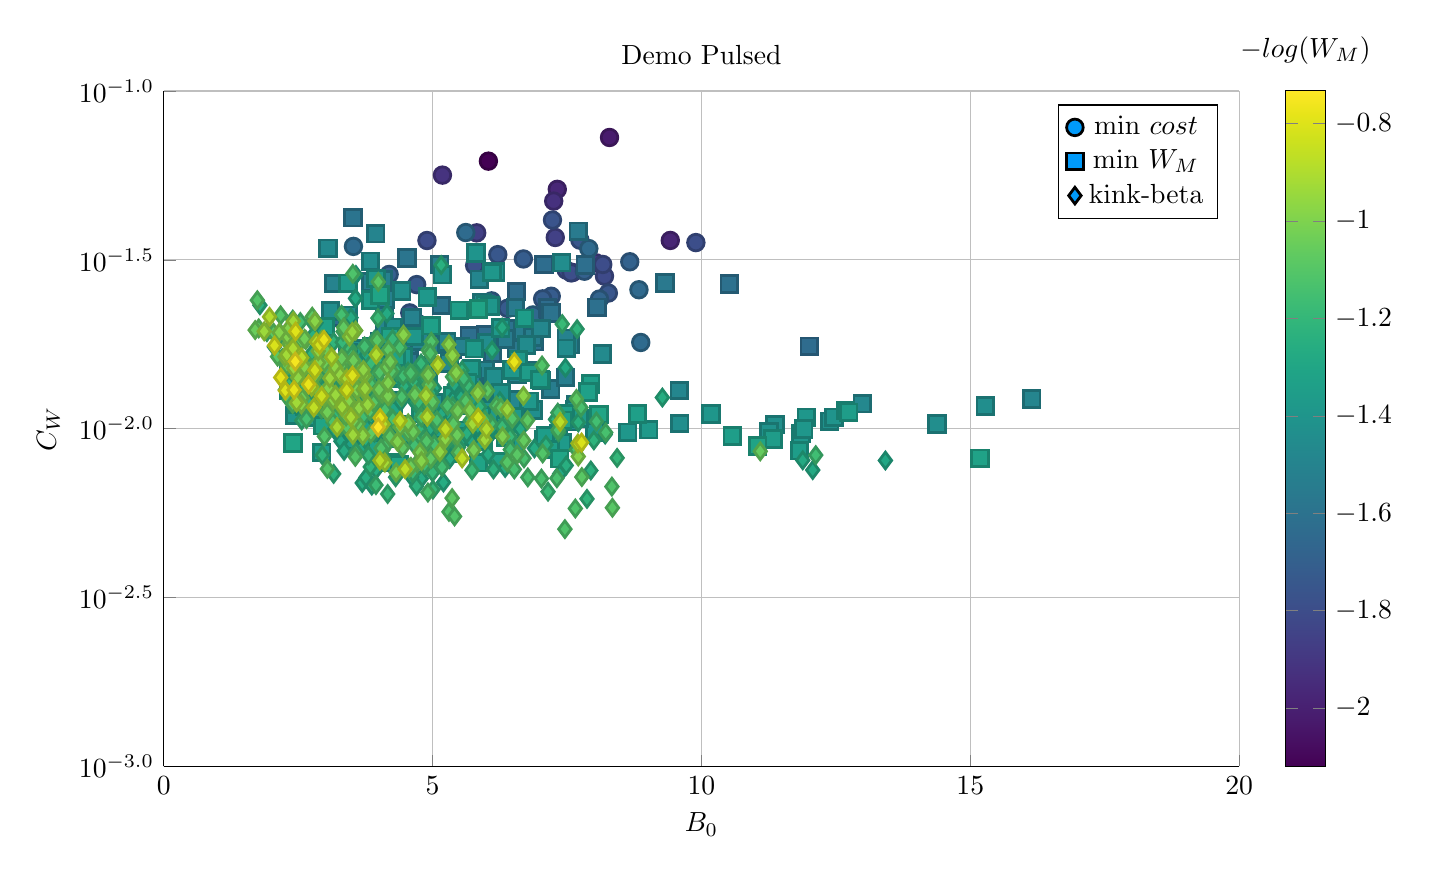
\begin{tikzpicture}[]
\begin{axis}[colorbar = {true}, height = {101.6mm}, ylabel = {${C}_{W}$}, title = {Demo Pulsed}, xmin = {0.0}, xmax = {20.0}, ymax = {0.1}, ymode = {log}, xlabel = {${B}_{0}$}, {unbounded coords=jump, scaled x ticks = false, xticklabel style={rotate = 0}, xmajorgrids = true, xtick = {0.0,5.0,10.0,15.0,20.0}, xticklabels = {0,5,10,15,20}, xtick align = inside, axis lines* = left, scaled y ticks = false, yticklabel style={rotate = 0}, log basis y=10, ymajorgrids = true, ytick = {0.001,0.0031622776601683794,0.01,0.03162277660168379,0.1}, yticklabels = {$10^{-3.0}$,$10^{-2.5}$,$10^{-2.0}$,$10^{-1.5}$,$10^{-1.0}$}, ytick align = inside, axis lines* = left,     xshift = 0.0mm,
    yshift = 0.0mm,
    axis background/.style={fill={rgb,1:red,1.00000000;green,1.00000000;blue,1.00000000}}
, colormap={plots}{rgb=(0.26700400,0.00487400,0.32941500), rgb=(0.27794100,0.05632400,0.38119100), rgb=(0.28291000,0.10539300,0.42690200), rgb=(0.28229000,0.14591200,0.46151000), rgb=(0.27619400,0.19007400,0.49300100), rgb=(0.26514500,0.23295600,0.51659900), rgb=(0.25042500,0.27429000,0.53310300), rgb=(0.23360300,0.31382800,0.54391400), rgb=(0.21813000,0.34743200,0.55003800), rgb=(0.20123900,0.38367000,0.55429400), rgb=(0.18555600,0.41857000,0.55675300), rgb=(0.17117600,0.45253000,0.55796500), rgb=(0.15772900,0.48593200,0.55801300), rgb=(0.14618000,0.51541300,0.55682300), rgb=(0.13374300,0.54853500,0.55354100), rgb=(0.12346300,0.58168700,0.54744500), rgb=(0.11948300,0.61481700,0.53769200), rgb=(0.12632600,0.64410700,0.52531100), rgb=(0.15014800,0.67663100,0.50658900), rgb=(0.19109000,0.70836600,0.48228400), rgb=(0.24607000,0.73891000,0.45202400), rgb=(0.31192500,0.76782200,0.41558600), rgb=(0.37777900,0.79178100,0.37793900), rgb=(0.45867400,0.81636300,0.32972700), rgb=(0.54552400,0.83803900,0.27562600), rgb=(0.63690200,0.85654200,0.21662000), rgb=(0.73088900,0.87191600,0.15602900), rgb=(0.81457600,0.88339300,0.11034700), rgb=(0.90631100,0.89485500,0.09812500), rgb=(0.99324800,0.90615700,0.14393600)}, colorbar style={title=$-log( W_M )$}}, ymin = {0.001}, width = {152.4mm}]\addplot+[scatter, scatter src=explicit, only marks = {true}, color = {rgb,1:red,0.00000000;green,0.60560316;blue,0.97868012},
draw opacity=1,
line width=0,
solid,mark = *,
mark size = 3.0,
mark options = {
    color = {rgb,1:red,0.00000000;green,0.00000000;blue,0.00000000}, draw opacity = 1.0,
    fill = {rgb,1:red,0.00000000;green,0.60560316;blue,0.97868012}, fill opacity = 1,
    line width = 1,
    rotate = 0,
    solid
}] coordinates {
(6.0376291897873084, 0.06197483174638786) [-2.119809409407475]
(8.29014098058992, 0.07282952610606806) [-2.022107373269494]
(9.420103794137964, 0.03609135913093006) [-1.9777667149411715]
(7.318722954994432, 0.051130362720294704) [-1.969913275543008]
(7.25219757869589, 0.047199699242522014) [-1.9276279243167613]
(5.1830212243548095, 0.05634035623848662) [-1.9180907603558137]
(7.605075373452645, 0.0290156978870517) [-1.8866814459155106]
(8.038027414173005, 0.030992141550921816) [-1.8810042714594786]
(5.819960412661949, 0.03801538835634297) [-1.861231108978198]
(7.281484484411212, 0.03683114347875789) [-1.8558362580925096]
(8.196367519793338, 0.028291519575269056) [-1.811508198071671]
(4.895214337316329, 0.03607745072820276) [-1.8048956433290855]
(8.164740419623248, 0.030644555029908985) [-1.797922304180305]
(7.485375190378305, 0.02949537628440487) [-1.7974494679074275]
(7.575835693873996, 0.028933124859920306) [-1.7961193741663348]
(9.896061646161176, 0.03557653455378664) [-1.7922955251500743]
(5.781753762991258, 0.030417392770278703) [-1.7763653379983415]
(7.2293817061271435, 0.04147970255534964) [-1.762574168304495]
(8.268196094729024, 0.025210912703269035) [-1.7524000959584443]
(7.738981336245074, 0.036173737778618126) [-1.7467043012053995]
(6.212564476265189, 0.032766263996239824) [-1.7445197156480476]
(4.575558741192934, 0.02202338694073385) [-1.7362913649987812]
(4.703832637956078, 0.026714074548194577) [-1.7340594740544224]
(6.392336735687798, 0.022713661122324157) [-1.7289223235866222]
(7.206811582654181, 0.02466928657304406) [-1.719614121069955]
(7.047211448521989, 0.024233508820652228) [-1.7167136137505041]
(6.688671457635685, 0.03181143352229567) [-1.7154437116459917]
(4.191978956537718, 0.028622291298276443) [-1.7060722509483957]
(7.823016295826839, 0.02926238447048653) [-1.6937830944780397]
(8.667006322370625, 0.03120868171359675) [-1.6889812321302553]
(6.097668524082785, 0.023905595143656186) [-1.686209077026567]
(8.103448360984764, 0.024204963735087338) [-1.6786883535604935]
(4.743339804248675, 0.020413682949498045) [-1.6734478593396724]
(6.86661111430788, 0.02171708878277083) [-1.650681965327452]
(8.837409416541565, 0.025789595420542006) [-1.6458495153344535]
(7.905189202860984, 0.034141771708853026) [-1.6412636709027566]
(5.617445394262159, 0.03809649700399676) [-1.6393314314904326]
(3.5279604177676442, 0.0346599142742729) [-1.6390302509540549]
(8.87108059531098, 0.018002375584230325) [-1.6381696948341165]
};
\addlegendentry{min $cost$}
\addlegendentry{min $W_M$}
\addlegendentry{kink-beta}
\addplot+[scatter, scatter src=explicit, only marks = {true}, color = {rgb,1:red,0.00000000;green,0.60560316;blue,0.97868012},
draw opacity=1,
line width=0,
solid,mark = square*,
mark size = 3.0,
mark options = {
    color = {rgb,1:red,0.00000000;green,0.00000000;blue,0.00000000}, draw opacity = 1.0,
    fill = {rgb,1:red,0.00000000;green,0.60560316;blue,0.97868012}, fill opacity = 1,
    line width = 1,
    rotate = 0,
    solid
}] coordinates {
(12.006327167234412, 0.017540808339758972) [-1.6348798048481208]
(7.13617498148303, 0.022785258097976623) [-1.6277277898588538]
(7.070736325233126, 0.030625514244526048) [-1.627684330571819]
(6.56017053121773, 0.025489957683783454) [-1.6248467182009472]
(5.980925581195891, 0.0189830433690413) [-1.62256122166559]
(5.681680569563924, 0.018838350678554387) [-1.6197529434592726]
(7.838353199376363, 0.030553347689269015) [-1.619473374550493]
(3.1599502425274832, 0.0213568595963161) [-1.6190205769362032]
(5.370255019403915, 0.017173711360022336) [-1.617478678707941]
(8.057787659408406, 0.022891816741403965) [-1.6135161817566324]
(10.515719243031652, 0.026834336105762403) [-1.6079101518459553]
(6.442976568556264, 0.01976733422078956) [-1.6005797137016178]
(6.892650960552643, 0.01811055755791537) [-1.5991182248913247]
(7.198509347079774, 0.02202289176749285) [-1.595836360479248]
(3.517726346433672, 0.042161103004000076) [-1.589397412964098]
(5.159769580238814, 0.0231728109038665) [-1.589205111302375]
(3.8365890735140322, 0.015450272567257462) [-1.5875377953010883]
(4.522678122476023, 0.0319953061173649) [-1.5845809864087244]
(4.56749863701147, 0.016164039710660088) [-1.5775674018565111]
(6.114630190971535, 0.016693759971981265) [-1.5713155071601692]
(6.555603899680141, 0.01726409176752251) [-1.5652457853616617]
(9.324368979144754, 0.02698353416604086) [-1.5643952661253622]
(4.546856339243231, 0.01769761001811183) [-1.5595601870169422]
(6.5407531731873325, 0.02281153437267921) [-1.552568848396255]
(7.709084001143297, 0.038423068705951594) [-1.5520441226990631]
(4.10568363851079, 0.022224095489930037) [-1.544925041354305]
(6.355103453558186, 0.01841847429182733) [-1.5430023738862098]
(6.679865116269665, 0.019477644457703495) [-1.5396243114452017]
(4.896210634322484, 0.01449908817629988) [-1.538692217528126]
(7.198003119281151, 0.013092644307368572) [-1.5373740781698282]
(5.131173117670862, 0.030574977212997605) [-1.5350312948909135]
(7.472740510067807, 0.014205258889817484) [-1.5317433014682034]
(6.8683725940871865, 0.018689708848548738) [-1.5311850486265117]
(5.766565183000099, 0.01387590038164943) [-1.5287451237254033]
(5.73965239781306, 0.013905952265261586) [-1.526526816139614]
(3.850247344392022, 0.027241135712482305) [-1.519178921439465]
(3.724681151757905, 0.016910779414334946) [-1.517891032933806]
(4.124143130105857, 0.024191852864153648) [-1.5130165343032327]
(7.561125230807454, 0.01773125993862434) [-1.5126055054907948]
(4.0802413603524945, 0.027530426264504002) [-1.5122759735909235]
(6.754598599599373, 0.014899481481132758) [-1.5121531835443067]
(5.140825889424527, 0.01778122202031051) [-1.5121518481580156]
(7.487694805484361, 0.01852162588841651) [-1.509963665969106]
(4.706543051446386, 0.013259386458548635) [-1.5098191352881933]
(4.023530685620901, 0.018078145365757758) [-1.5094600237705913]
(4.619206299311601, 0.02134336001409843) [-1.5091677016781566]
(5.515733266875538, 0.017507453096671365) [-1.505813383704145]
(3.1665229051711936, 0.026909424888676328) [-1.5035180904231982]
(4.7606297434625375, 0.018116695499993292) [-1.4998070828001184]
(2.6908911342489987, 0.01226652304303364) [-1.4993412700061268]
(5.9813285749518785, 0.014898889997617197) [-1.4970388348465338]
(5.73832856833363, 0.014279317114283529) [-1.4968151314329754]
(3.9410419383640107, 0.03778412752723575) [-1.4959262215207656]
(3.430490492055365, 0.012007443130458324) [-1.495878750102406]
(3.3992707879943804, 0.014131383104205364) [-1.4911760171512294]
(3.8869352833553514, 0.013847785437885679) [-1.4909012021072667]
(3.492353905872561, 0.013113327535403696) [-1.4904727997922445]
(16.140534236107158, 0.012253217681920671) [-1.4902975254497872]
(4.106645540108447, 0.020179920200301855) [-1.4899596862430686]
(6.569539440995961, 0.014465480638895564) [-1.484315053758591]
(9.588346294205625, 0.012974868808400592) [-1.4832272441818983]
(5.870682126151471, 0.02767164571202513) [-1.481908947186888]
(3.925275118526448, 0.012700241486954703) [-1.481610811848838]
(5.262489226894273, 0.018066556725317685) [-1.4808315890609627]
(5.861692393922073, 0.012152582495637852) [-1.4803924190961808]
(5.918313590579109, 0.023591043628319753) [-1.4777813991456452]
(3.8833429023200345, 0.014987126189756067) [-1.476226145125234]
(6.481366220083333, 0.012179602718049342) [-1.476103765156545]
(7.019026450980214, 0.0198044997246676) [-1.4759532635696884]
(12.992560883586702, 0.011854698849849837) [-1.4744693843941874]
(5.3126270403520905, 0.015665176708494814) [-1.4721189566530006]
(4.653270023129369, 0.012892988065699775) [-1.4694765884704042]
(5.56336817143885, 0.011723605612914264) [-1.4684762544315009]
(5.887370453127917, 0.01146148363735155) [-1.4673712598422484]
(4.769173324013478, 0.01403086783418577) [-1.4665127712450712]
(3.0555463671233567, 0.03422172209265897) [-1.466465342676487]
(7.658132277548963, 0.011814056076879775) [-1.4656409913573911]
(8.15735419014013, 0.01666169164744686) [-1.4607639902508311]
(3.6997605874700903, 0.011797068547740396) [-1.454804800167485]
(6.7465287199750925, 0.017714850999176746) [-1.454016548396377]
(7.488515154319888, 0.01730924236440855) [-1.449126660054787]
(4.899466318563284, 0.015350811156516968) [-1.4450317564339483]
(7.901350621283068, 0.010700521525178483) [-1.4442476160174416]
(6.002415704010382, 0.017999193081243068) [-1.4428695943470562]
(3.846424137063846, 0.03129913412451443) [-1.4416527786165851]
(7.401783272746636, 0.030992801350489627) [-1.4412978501823663]
(7.020304767734094, 0.013876797144792313) [-1.4410674847520173]
(14.381919368485658, 0.0103371343106061) [-1.4407593364531412]
(3.1028814474410384, 0.022291694526716137) [-1.4382523340904476]
(3.7705732972432857, 0.011033535668865918) [-1.4374618391296154]
(5.967712362691083, 0.011578760205733224) [-1.437309497392895]
(6.135496498952566, 0.014225493350487712) [-1.437004502630189]
(15.280361971651645, 0.011662685993065088) [-1.4369516286418977]
(9.595768152006077, 0.010363517857158673) [-1.4359296968945898]
(2.706516860566676, 0.012593943496598788) [-1.4348111698815942]
(7.531253395446069, 0.010486068251726523) [-1.4347403934029699]
(6.873696165627944, 0.011351647420548932) [-1.432162507533083]
(6.006312634325258, 0.010703895251080882) [-1.4298959659652046]
(11.369550336874795, 0.010279170294604838) [-1.429141349371285]
(4.426279201300683, 0.025557043779995653) [-1.4288294492620477]
(4.273188204709541, 0.019981046165081038) [-1.4275892047251812]
(3.284854781128933, 0.014011150106021747) [-1.42664672926539]
(3.563101077929043, 0.017276630179413652) [-1.4239039330716527]
(7.65153347612068, 0.01135063897630595) [-1.4237047673472223]
(3.427537242139707, 0.021651736693319764) [-1.4220880228019461]
(6.174362312871966, 0.029124606257697153) [-1.4214589216983458]
(12.38255150794347, 0.010524080735331771) [-1.4192750546166355]
(3.96419825273711, 0.012152497168515361) [-1.4188846212567885]
(4.984822443753677, 0.010654264771940928) [-1.418142111238707]
(4.177511278387798, 0.012093014306414056) [-1.4175771687309422]
(4.494983202230982, 0.010307835186267926) [-1.4166515403180218]
(11.258702848316975, 0.009802839106844477) [-1.4151591623618127]
(4.167168689552534, 0.012089411129630757) [-1.415086999740124]
(3.4268121903746978, 0.016771907819218872) [-1.4150518254702726]
(2.3537099631543916, 0.01479570625667246) [-1.412750376425469]
(5.182420388292304, 0.02858609969916251) [-1.4118418857799215]
(3.927997304454704, 0.009976658176736495) [-1.411745253778192]
(5.018593701573295, 0.011899859669740264) [-1.4101129990450592]
(3.885531120492574, 0.010975696046095008) [-1.4098064292280077]
(5.2474162565909435, 0.010078193568331789) [-1.4071217370506766]
(6.2004105061477235, 0.012567870805096065) [-1.4069653518342513]
(12.464033848113864, 0.010809590548122633) [-1.4053188021751997]
(3.762648000098064, 0.013228123351848638) [-1.4040831795581317]
(3.7635564019241006, 0.012756284815624411) [-1.403783408224447]
(6.2439977027647595, 0.011849909135487101) [-1.4034059706684434]
(4.011269493628918, 0.015391572104901911) [-1.4031334212883295]
(5.948372401188327, 0.011370525417095621) [-1.4027031557706915]
(6.105240096014571, 0.010883116023126084) [-1.4023409214316394]
(5.807785740293634, 0.03314304390232683) [-1.4018234466267534]
(6.240369813761391, 0.010943279854872806) [-1.4001967788421508]
(6.270554586884656, 0.012776602146795163) [-1.3983213447403338]
(10.178788051574003, 0.011065372696240975) [-1.3946316971345938]
(7.342798909437036, 0.009697674748088487) [-1.393981306323598]
(5.515659388841616, 0.012316212001497684) [-1.3939743444895971]
(5.981611630666005, 0.023293627402023516) [-1.3938659098694006]
(3.371060773893557, 0.012799262525216688) [-1.3934317035795]
(6.064709438936184, 0.02306752096780418) [-1.3919378361313393]
(2.855332574063217, 0.011575943181240602) [-1.3913501343623875]
(2.4437405695506387, 0.010938935413839007) [-1.3899986150261634]
(6.469695877217161, 0.014916276865219583) [-1.3888953225499234]
(11.950718647766315, 0.010811642128190005) [-1.3883849558567678]
(5.747775187553233, 0.012086573842968483) [-1.3880683151937296]
(8.62770676217042, 0.00974951527611275) [-1.3879257169733152]
(4.661434120932319, 0.01875474559032549) [-1.387200255154835]
(6.101706649362307, 0.028992717747430105) [-1.3869139374162498]
(4.921653466094031, 0.014275341697562267) [-1.385982080919773]
(11.85196051673142, 0.009658736241223327) [-1.385951966541943]
(11.902146743793873, 0.009979205376142167) [-1.384341496966052]
(8.017011891149473, 0.009781750047901397) [-1.3836628266676982]
(3.9453588859348705, 0.027837899406166513) [-1.383138617240496]
(2.7450573045264335, 0.013692957043690078) [-1.3831333668949872]
(6.793555399638037, 0.012055028195149642) [-1.3823755173012382]
(4.903012581972081, 0.02457168150365556) [-1.381386436684111]
(3.8233047461789904, 0.013467436970042478) [-1.381013926041926]
(3.9360749856112256, 0.01632900764605371) [-1.3807582017142732]
(4.3204944514848105, 0.016233342907168043) [-1.3795912650626003]
(6.26763114858317, 0.019856726760879642) [-1.3784744825946547]
(9.017994817618085, 0.009937020814786353) [-1.3784050115817357]
(5.662871931648498, 0.012947457233964572) [-1.3727350903904059]
(3.423561741004342, 0.02692798924274793) [-1.3726382795387042]
(6.527451391525709, 0.00894061047284123) [-1.3726183217257064]
(6.511799045245276, 0.01083618948017438) [-1.370506635821487]
(6.061861020595905, 0.010820381028973857) [-1.3702834841058706]
(5.720454003557526, 0.01507474130083674) [-1.3699905172740252]
(6.595551058907596, 0.016024901755414496) [-1.3694510931398833]
(7.0656961487120595, 0.009286958803152093) [-1.3690194932725448]
(5.7756989121996005, 0.01725165686414962) [-1.3685993689556193]
(7.407124185747266, 0.009100422809121853) [-1.3680782620249432]
(5.940087524048422, 0.009358898748733285) [-1.3659937757563743]
(7.721929512311208, 0.010741593794976297) [-1.3655266043175585]
(4.375024347794328, 0.00935804014953258) [-1.365489135635999]
(4.45788760453061, 0.01631624677926724) [-1.365314944668722]
(12.678530079731434, 0.011316654652064283) [-1.3620488306806053]
(2.8403626573133516, 0.010811158792461435) [-1.3600883836878876]
(6.791476575808721, 0.014663988794896813) [-1.3569999482959285]
(11.332959766691456, 0.009327975573933072) [-1.3565369493574833]
(3.5993697558328135, 0.009591330831744169) [-1.3564434514013937]
(7.094333669876596, 0.009510520762087537) [-1.355670949654743]
(11.824184374151493, 0.008600603815848054) [-1.3550689180362785]
(6.708017904184935, 0.0212306523206366) [-1.3545717493575382]
(3.9462715514882833, 0.011027495783414606) [-1.3536406793714741]
(3.846707059253749, 0.02403578580290836) [-1.3522480304376618]
(5.54278675314685, 0.01277987363566607) [-1.351683168790268]
(12.739777598462709, 0.011181317227288103) [-1.3509416538039447]
(6.996720111065061, 0.013988110662625983) [-1.350917699634303]
(5.58993729043943, 0.011706003302806382) [-1.3498675794038522]
(3.872376016258126, 0.01744787935363008) [-1.3480954361555229]
(10.572844829384726, 0.009513333911267541) [-1.3474307155472665]
(2.938257234568377, 0.008506399274340092) [-1.345835600508895]
(5.495169200054534, 0.022402494346273383) [-1.3441619287129023]
(3.5507214607316238, 0.011568935524735228) [-1.343173024895477]
(5.504907463368559, 0.009888039453025594) [-1.3431102335422052]
(5.65163629087646, 0.013676025720795522) [-1.3418959513921676]
(7.466637754651223, 0.011055478792069253) [-1.3416390955818198]
(7.940566023194332, 0.013562184857025608) [-1.3412225668983788]
(4.645128912048539, 0.013928329166195007) [-1.3411223781363122]
(3.5178351993254204, 0.008957609956171385) [-1.3409980727589041]
(8.80912527255541, 0.011061155580644737) [-1.3407774046291352]
(4.414263871815846, 0.014142372730384274) [-1.340736718067575]
(3.5324039876905395, 0.014931289500105476) [-1.340172101894623]
(7.191161190692271, 0.008673821452175847) [-1.339371225527388]
(7.889566195214564, 0.012851757813003692) [-1.3355889626958743]
(5.053734570947225, 0.009585198585080813) [-1.3353537500446666]
(3.197632928999906, 0.011502571386254939) [-1.3352936153265889]
(4.973690447707013, 0.020177908654106694) [-1.3347167954999664]
(5.902248798024801, 0.010934192827515073) [-1.3333464153994234]
(6.352797677366824, 0.010187040046408826) [-1.3319467069356516]
(5.715498297799574, 0.012093243108414115) [-1.3317606682979195]
(6.242863088777295, 0.0099544891977854) [-1.330878268232421]
(5.056377266744529, 0.00892167491417854) [-1.329838199225075]
(3.0039565360029306, 0.020024514359414238) [-1.3275817805394716]
(3.774870490274173, 0.010377685225384297) [-1.3271981479523673]
(3.4560894708307504, 0.00923521460571462) [-1.3257753666633474]
(3.739062356737302, 0.016536435428404248) [-1.324805801675252]
(15.176586722658566, 0.008177838551829547) [-1.3236480395933032]
(3.419819319784293, 0.01320289357034274) [-1.3223872875360454]
(6.352130677917973, 0.009416665871049234) [-1.320790714548859]
(2.322477510691322, 0.012966997564871513) [-1.3198610091294973]
(2.324248942944489, 0.014941915896507264) [-1.3173999901029887]
(4.846244775501472, 0.014705731648914599) [-1.3172398911361078]
(4.214745039825576, 0.018745840734049092) [-1.3155841266914403]
(11.045339988929378, 0.008883845818604448) [-1.3144429555765318]
(4.3255410851853195, 0.016334708642476756) [-1.3140984246311314]
(6.235375099026929, 0.007999169369094802) [-1.3136141988883636]
(7.418567204666788, 0.010593671042148305) [-1.3130409307938926]
(3.522574707719547, 0.011696426000066894) [-1.312883593567563]
(5.395063115984087, 0.008437215022084032) [-1.3113636666391015]
(2.9623590695188793, 0.010210442889078589) [-1.3110543205827916]
(2.619151065722938, 0.01161135507437133) [-1.3101666476591896]
(4.251202424158484, 0.010715857251244127) [-1.3094281744638252]
(5.850851943214601, 0.007935513211517508) [-1.3092819198295769]
(2.800331008488367, 0.01527961135499392) [-1.3091789421820008]
(3.962750439094108, 0.008718673720708605) [-1.308657609117127]
(3.9491153183500765, 0.012115862676003172) [-1.30815684782275]
(5.368732790803233, 0.012528702800938256) [-1.3073192126014976]
(5.531029878673032, 0.009466859805614364) [-1.306104667504652]
(4.019577892699671, 0.024862203238592617) [-1.3061029424340123]
(5.854899512854821, 0.022588731344076834) [-1.3059932173472433]
(3.4111150555142538, 0.010067194372351543) [-1.3053424100316993]
(5.9474935100169155, 0.009194414774426339) [-1.3048906180553326]
(4.442986113810117, 0.014224364223609164) [-1.3043596581137094]
(4.484605690017701, 0.00966642720928779) [-1.304157201921016]
(4.235072291257464, 0.007934056288357859) [-1.3040523349428945]
(2.481542761360737, 0.011830250137913223) [-1.3039439069452712]
(7.36295762251903, 0.008152912507864905) [-1.3022467953572583]
(4.272648359589559, 0.011323662495891916) [-1.3012176243848619]
(2.403751630196505, 0.009074217857747638) [-1.3011866801418175]
(8.097817905088668, 0.011011974496683653) [-1.3004916659282275]
(4.379478185125185, 0.007824745570931163) [-1.3001880033121107]
(4.787155359091795, 0.011078402389842862) [-1.2993649239636758]
};
\addlegendentry{min $cost$}
\addlegendentry{min $W_M$}
\addlegendentry{kink-beta}
\addplot+[scatter, scatter src=explicit, only marks = {true}, color = {rgb,1:red,0.00000000;green,0.60560316;blue,0.97868012},
draw opacity=1,
line width=0,
solid,mark = diamond*,
mark size = 3.0,
mark options = {
    color = {rgb,1:red,0.00000000;green,0.00000000;blue,0.00000000}, draw opacity = 1.0,
    fill = {rgb,1:red,0.00000000;green,0.60560316;blue,0.97868012}, fill opacity = 1,
    line width = 1,
    rotate = 0,
    solid
}] coordinates {
(3.5121202416558273, 0.012133883145293747) [-1.2971735267311564]
(5.277662377204398, 0.008497507185750146) [-1.2963451470925318]
(4.933311521981375, 0.011968595839803002) [-1.2939289874566402]
(13.420827419108324, 0.008051203599652048) [-1.2928570974581939]
(5.71174352009151, 0.009198462479520332) [-1.2926592596370523]
(5.012096245785827, 0.009976448637174172) [-1.2918359622137705]
(3.8248114438663654, 0.011200517330116096) [-1.2901565279273088]
(2.959247673493197, 0.014778677283745992) [-1.2885231243501492]
(4.219667355934983, 0.009645840422057206) [-1.2873870680148987]
(3.9368699206088387, 0.015368153744705897) [-1.2867189599495152]
(5.3763072490644115, 0.012200186404574626) [-1.2866608738447551]
(6.009303119414782, 0.009314200607444962) [-1.2862989627940875]
(7.363118579080014, 0.007351086075188858) [-1.2856479743658245]
(4.035860790767533, 0.011184811263709776) [-1.283461572944208]
(3.5737740510711875, 0.028511756618296732) [-1.282628142229196]
(3.295672492906566, 0.0091809969411667) [-1.282318795548118]
(7.469892811394071, 0.015147418693115068) [-1.2809419797501462]
(3.716712298492769, 0.009441743395354373) [-1.2802239523296417]
(5.842646483303914, 0.010115067051441084) [-1.279661807174519]
(3.655882587201946, 0.008682653521467484) [-1.2793586996677089]
(5.000424842433475, 0.00919694313697991) [-1.279241431080542]
(11.883710143751259, 0.008062649665833432) [-1.2791738597664242]
(3.769661149622435, 0.016537125137685977) [-1.2777724695025643]
(3.565755959498115, 0.024311609583825906) [-1.2776560252665474]
(12.069034139998493, 0.007543708329813699) [-1.2776226586446298]
(5.402872542958727, 0.013472425466080754) [-1.2772080908839465]
(3.5721530790668217, 0.010591022499429533) [-1.2768888641183538]
(6.113391779890812, 0.010068814155906535) [-1.2749252706301877]
(5.281892154588248, 0.011122028940902477) [-1.27405635520294]
(2.8318856035975837, 0.020592443763116842) [-1.273999627133777]
(3.171270658752047, 0.009932693135460512) [-1.2739263340884897]
(5.035138050414791, 0.013177764718534145) [-1.273686836355838]
(4.151495259485247, 0.021930543698997433) [-1.272060671091855]
(3.9079897018955214, 0.01703366147805158) [-1.2717552020206426]
(3.0490838025892786, 0.013199694993892157) [-1.2715552113887816]
(3.026643094075235, 0.018137179053328113) [-1.2711256143593725]
(5.509559307824704, 0.009089213335736035) [-1.2706918059143955]
(6.2933025717891, 0.019922160606497104) [-1.270659241243097]
(8.209845211268025, 0.009612072783370788) [-1.2706266042708976]
(2.738511903007871, 0.011815687417752718) [-1.2699973230973551]
(5.3168436208878225, 0.008127375094877596) [-1.2694883213650459]
(3.8713710824000858, 0.011108460101523684) [-1.269469949244091]
(4.40489854224676, 0.01200413289507089) [-1.2693810054133523]
(3.4817589149659844, 0.021322131632939743) [-1.2685038799823198]
(6.893437951158227, 0.008746022086925008) [-1.268011220133286]
(6.250792601428729, 0.012071261699451271) [-1.2676767161765092]
(3.8480774904528383, 0.015027760071695463) [-1.2672360183442966]
(5.528072317285266, 0.012386782250268949) [-1.2670329245716005]
(6.631542703995221, 0.00997135774995843) [-1.266521603924258]
(3.402074742995083, 0.014743359804979298) [-1.265829536383991]
(5.157191379781698, 0.011015221663609409) [-1.2655850749955841]
(4.081908569510066, 0.009754591610171831) [-1.2651606387913807]
(6.032688069883985, 0.008391084675782472) [-1.2650267302153226]
(6.323926257057424, 0.011459660264397842) [-1.2643165163116283]
(5.673390538312956, 0.01314380020899071) [-1.2638630587832318]
(4.962600203221328, 0.0100188505842072) [-1.263682663264664]
(5.202158247710273, 0.006930908540990179) [-1.2635507051033026]
(6.3498106860494135, 0.007655768190498255) [-1.2630930817893484]
(3.3542410941806997, 0.008595102325139414) [-1.2620028969039807]
(5.408801595842229, 0.008993269936185943) [-1.2617711256664215]
(4.060468748765856, 0.013435175267701598) [-1.2607622270815175]
(4.3458863312043015, 0.010399130132164968) [-1.2599969566754825]
(4.941827638049582, 0.011066872440514844) [-1.2580199333772297]
(3.7865968807980463, 0.014164623239439114) [-1.257674742909116]
(3.8700982106168342, 0.006784814729690784) [-1.256920205986828]
(3.860117954844053, 0.010847484174753686) [-1.2558826127376497]
(4.667259329944255, 0.012006910499828622) [-1.2545784323742915]
(9.273036766388604, 0.012367303307791636) [-1.2541769145790829]
(3.6923348872456994, 0.006909773766752695) [-1.2538081670568602]
(4.789726542521002, 0.007118806510545466) [-1.2537331036632384]
(3.7600070371379886, 0.007163920014099904) [-1.2523947287534352]
(4.421298005693511, 0.01409766195530951) [-1.252161894882265]
(4.610630866671953, 0.007191926525759095) [-1.2517841257242934]
(5.20128149593585, 0.010140660180167243) [-1.2510148685101052]
(4.053725242509742, 0.009947685467565285) [-1.2503817284236358]
(3.9490509942400003, 0.00755783116205777) [-1.2500618007814928]
(6.105587908907182, 0.01705584468677382) [-1.249408930050928]
(7.485181266118961, 0.007782048369656626) [-1.248434923528094]
(5.429695722081377, 0.009638865392082259) [-1.246475793101881]
(5.6359771653268504, 0.009668090359024908) [-1.2453083223674235]
(3.585647465370671, 0.01181801423349667) [-1.2430271033455136]
(4.967782040145293, 0.012765537294567253) [-1.2425009663963265]
(2.836991692259108, 0.014096920088512531) [-1.2420036959161107]
(3.851942066673645, 0.014638041989732616) [-1.2406291651922927]
(3.86783106759803, 0.011330221246013529) [-1.2404081246835275]
(4.144235850020982, 0.009882346466549934) [-1.2402721066912186]
(5.159714665590853, 0.030517882462548936) [-1.2399829928026451]
(2.7744066236166, 0.018855374361929193) [-1.2398403601837327]
(2.9616080503895255, 0.013105067185166342) [-1.2382227382575577]
(1.789190176158448, 0.023206171452307512) [-1.2372685823332665]
(2.057072816922599, 0.01748239328622686) [-1.2369979991721363]
(7.709371728502172, 0.010436966421480154) [-1.2364971528125899]
(3.754765214297292, 0.00929031971105747) [-1.235918342000411]
(2.4390459870956867, 0.01224311754662533) [-1.235332112263366]
(4.477287158856502, 0.013377000135851953) [-1.235230354209212]
(7.942543848452732, 0.00752176857171885) [-1.2348662947331168]
(6.132444327284232, 0.007577390318458053) [-1.2331237451825037]
(7.107404657748289, 0.008954934736687754) [-1.2314216648450123]
(3.1603738338503238, 0.007348723496235854) [-1.2276908244938955]
(4.701751679050523, 0.00675688814735783) [-1.2234874983546444]
(3.1402652758611795, 0.01611655322423877) [-1.2224132121245386]
(7.999091158540905, 0.009234491873309686) [-1.2212129344183997]
(3.445549117779653, 0.012691970303684906) [-1.221000044288545]
(3.3885426284661953, 0.011032294768272291) [-1.2201668573985105]
(5.5456091712090725, 0.014875616723151944) [-1.2200113852982524]
(4.54243872092666, 0.014755597501979523) [-1.2200110437170943]
(2.4705292036298423, 0.015480160187022769) [-1.2199386530853975]
(7.687093361817087, 0.019725018407248666) [-1.2192027637421239]
(3.3454463511646835, 0.01227428321856098) [-1.218844626416703]
(2.8137615251130303, 0.013727476887235461) [-1.2187513907488479]
(4.312486225133877, 0.007184219051293641) [-1.2182120816961266]
(4.772997377730909, 0.011425165896800414) [-1.2178523450390264]
(2.7578042878780122, 0.01671459075301228) [-1.217564445140848]
(3.8197074658287047, 0.01316079396243774) [-1.2148287908302686]
(7.285303183831831, 0.010653867811546877) [-1.2144650329368094]
(7.87104962823073, 0.006198307301760009) [-1.2142295699793069]
(3.9206245950101466, 0.009725241928162248) [-1.2114971471794018]
(2.949515743068061, 0.00834877000609595) [-1.2110590840755884]
(6.340610180985918, 0.010394495894857034) [-1.210956786812969]
(5.875295019857379, 0.01160689504064373) [-1.210625479626572]
(3.8412979296256804, 0.007709496307162327) [-1.210548450407708]
(4.861863097960495, 0.01196700634860152) [-1.2101072964851303]
(3.685725743106405, 0.014267222031421351) [-1.2097043828037173]
(3.0450965804813084, 0.017649120721508472) [-1.2090548152300868]
(5.178245200408863, 0.00786922573538261) [-1.2089432452477198]
(3.1609089410843576, 0.018050177035811292) [-1.2088567702310062]
(4.648811455834014, 0.01374396978202603) [-1.208355792529063]
(2.6748681285923954, 0.012119563498851512) [-1.2079597098695036]
(3.4809700733273528, 0.01476620759208673) [-1.2069143247822283]
(2.5693210089699696, 0.014425121215984256) [-1.2060355587049236]
(5.48357638584481, 0.008818373193963157) [-1.2051439881244612]
(3.5314903256684156, 0.014347196234709005) [-1.2048202874468241]
(2.7372435536225725, 0.013090961135950088) [-1.20412102013171]
(8.431693660708335, 0.008195788944222735) [-1.2006084749599055]
(3.22168634343002, 0.011017845567179161) [-1.1997509076464346]
(2.71871093880185, 0.01471498897475931) [-1.1989561148134826]
(2.566609676009112, 0.010576750792174504) [-1.1977552093777106]
(3.976434539417637, 0.015955953274896677) [-1.1973464324024234]
(4.873125471162229, 0.014024797653122234) [-1.1952843257986516]
(4.765913327506254, 0.009913142251828634) [-1.194608172565493]
(4.100942713127369, 0.012231614304186931) [-1.1943983553124515]
(3.211186770718166, 0.012895825589119291) [-1.1943709063726027]
(3.8064949992758947, 0.008341248647504823) [-1.193465520169887]
(5.000301151056601, 0.007422215660710276) [-1.1934529196767811]
(3.320155156974005, 0.018029259293378272) [-1.1932608414538086]
(3.75169525130439, 0.01475503745943627) [-1.1930245850534404]
(4.785428924434849, 0.01559839957452813) [-1.19275308105931]
(5.006411779829835, 0.006601321305241876) [-1.1925650410586528]
(4.729161558851959, 0.012849471675853265) [-1.1916847830033912]
(4.164290783750659, 0.006406786662781295) [-1.1906829642457115]
(3.8087569173433318, 0.015231829402577652) [-1.1905171502567853]
(4.25698051374954, 0.018424630927819426) [-1.1868792227109848]
(3.5466435162495946, 0.012087057868798792) [-1.1860893620286155]
(5.358611559304756, 0.016048418150957987) [-1.1858875370196502]
(4.738906273187223, 0.011972397837837176) [-1.1854558952607928]
(2.328150699298343, 0.013483711604703155) [-1.1848213366225184]
(3.6344930189881155, 0.011761816070313931) [-1.1847475832442582]
(4.630903293878455, 0.007399398212169979) [-1.1837916630431773]
(3.5912206702417406, 0.010413257435217902) [-1.1834175022102877]
(6.439604151254825, 0.009470444499328991) [-1.1831305353511883]
(3.8587290599416177, 0.015647472969860403) [-1.1828511911535706]
(7.410839889439496, 0.020407456319850734) [-1.181840770808167]
(7.14687725893768, 0.006510208938595967) [-1.1814651012301538]
(6.293989671314393, 0.010147346100150811) [-1.1809344434678004]
(5.074144294813995, 0.010306295906351105) [-1.1788261142099545]
(7.342502353808642, 0.00975845363999315) [-1.1783873972417303]
(3.983645541941601, 0.021255557406142055) [-1.1773891261145735]
(5.733227859571759, 0.007530050850229014) [-1.1772489110999693]
(4.863020029854074, 0.008856286376022381) [-1.1771937197283155]
(2.752607478621478, 0.02079595788529988) [-1.1768483795316644]
(4.34034532964977, 0.01477464262853022) [-1.1754670828809672]
(5.651026413557157, 0.013447350775475101) [-1.1748259721272571]
(3.5729145749442672, 0.008533818365309384) [-1.1743579362801864]
(4.828275081463438, 0.00926629982316415) [-1.1731424023398116]
(5.256321718375727, 0.009127162071787865) [-1.1728411497954707]
(3.9468845539429505, 0.006808109484569134) [-1.172547785671985]
(3.524962730858139, 0.009974514104150454) [-1.171293732602548]
(2.4431003187410245, 0.014894587057756483) [-1.1706435645347975]
(3.366739715078965, 0.014934801738779929) [-1.1704804143126533]
(3.919159617305408, 0.018312728464608994) [-1.1694340492000508]
(3.985672010289093, 0.013038425730797958) [-1.1664836698360914]
(3.9602939466659524, 0.011350876468389677) [-1.166021933665907]
(5.57816396320116, 0.014066615859663486) [-1.1653547583030963]
(3.7135886044363273, 0.01085952514652926) [-1.1637013339225117]
(3.732292225677101, 0.013377410828925157) [-1.1629231949973953]
(2.810904316594346, 0.013971916288186385) [-1.1625677338545028]
(3.034206239153093, 0.01498663044146402) [-1.1615160270969884]
(3.928029894091704, 0.011904820041118874) [-1.1613847421954753]
(2.6232376070221903, 0.013362365525672213) [-1.161380763910868]
(2.181980964430949, 0.019049310191542535) [-1.1612715538980343]
(3.2907142155592495, 0.010122141818818486) [-1.1608808882180581]
(5.371075061307033, 0.011629604231527799) [-1.1602959592128257]
(4.087463063508947, 0.008169777889897055) [-1.1601187846950554]
(12.12505747378403, 0.00834966465898116) [-1.1597072302883453]
(4.633851247354028, 0.014522157751088465) [-1.1596295654776811]
(4.45330922540737, 0.014324434384547807) [-1.1584930595938716]
(4.978980932820263, 0.008145962416336265) [-1.1583013384515075]
(4.072239550506503, 0.008646050418225202) [-1.1578217536561153]
(4.85035182175716, 0.007816314398845932) [-1.1564044749404534]
(4.69723552523336, 0.009241849076330648) [-1.1562110876559482]
(5.176056215218096, 0.007695271029389756) [-1.1558406723410226]
(2.324733000713789, 0.015939165384127457) [-1.1551976368183803]
(8.046084775778542, 0.010505037613581628) [-1.1547723960660046]
(3.463079612931359, 0.01720072822154318) [-1.1547042721803664]
(4.667433759545879, 0.008918107308299703) [-1.1544971334332936]
(7.328473923137891, 0.011156083675037292) [-1.1514583143146417]
(2.3995830140586842, 0.021035989307587558) [-1.150606587165903]
(3.735684839444669, 0.017520815218592205) [-1.1497568820513546]
(1.9186754281020504, 0.019315926185319167) [-1.1488471764736738]
(3.495720099796872, 0.016442878704583205) [-1.14854127278881]
(3.3507099367400888, 0.0147653907680726) [-1.1481443824350337]
(2.5403709550525817, 0.02069244645197561) [-1.1475056240535222]
(3.307281211177642, 0.021750535713550727) [-1.147314943378139]
(2.9349707147715516, 0.011413531346774588) [-1.1452162507505037]
(4.961675340508142, 0.011657490769208391) [-1.1440985305669964]
(6.445744456978382, 0.008671087589979474) [-1.143892607737901]
(5.031670650768643, 0.008990361186615302) [-1.1425154271844815]
(3.2137147299766298, 0.012558201977665608) [-1.1419282223298928]
(5.70066075923312, 0.010576229210216307) [-1.1414111342865825]
(4.790896832026144, 0.010807673225691976) [-1.1409606377195203]
(6.081644185908986, 0.010350872866134037) [-1.140632380055554]
(4.262584437785491, 0.010685556097930418) [-1.1405059694207205]
(2.655348617855336, 0.010680444710790922) [-1.1402761489506106]
(4.884538532888361, 0.01443507208815689) [-1.1390460916159142]
(6.52011178404498, 0.007579718089160525) [-1.1390342976608838]
(8.219749035826943, 0.009743368571375198) [-1.1383859727853913]
(7.7593463773798765, 0.011556690979889052) [-1.1378233474839952]
(4.388904498390582, 0.01739508549026366) [-1.1377132966757475]
(2.87524697467844, 0.011726874929476301) [-1.1376503199229564]
(7.024157829306849, 0.007116540390245059) [-1.1370921105287648]
(3.8400502604153073, 0.013630883580602493) [-1.136359546149739]
(2.4136732196953496, 0.01526251681202216) [-1.1362968805162]
(3.335636087343369, 0.019391120833403556) [-1.1358988321292471]
(3.77790333569627, 0.011860427509089479) [-1.1358539207185072]
(6.699557534343957, 0.008170611753766615) [-1.1356493088623822]
(6.7708197765220905, 0.007176648981252689) [-1.1354932328782563]
(7.311852681214439, 0.007134995489417047) [-1.1335001124055868]
(4.114267644468652, 0.011362840629455528) [-1.1323762690185122]
(4.590968546060674, 0.014605309967466338) [-1.1314565774222176]
(2.262672175094441, 0.013041177771875015) [-1.1310401855629826]
(4.912560401468473, 0.006470994712702174) [-1.130758874865596]
(4.425797376165855, 0.01241454353087534) [-1.1307392487451149]
(5.276947328747049, 0.011706749993287805) [-1.129690412643984]
(5.081053708467179, 0.01058602765458819) [-1.1289684185709847]
(3.1092112052594736, 0.016110870179123358) [-1.128250192514324]
(3.9460119406257674, 0.012109336313631335) [-1.1252475037678356]
(4.11423481085022, 0.008853551975990904) [-1.1245713568718563]
(7.673924172524263, 0.008673362533302236) [-1.1245104109679405]
(3.148239982482193, 0.010444270942938963) [-1.1242443075431308]
(7.332926397268772, 0.009907337069737673) [-1.1228938533825863]
(2.2060310557580083, 0.01617284927660436) [-1.1226570193988834]
(5.971667930097295, 0.010615516830489545) [-1.1219052279962924]
(3.51663552302443, 0.028747991383312018) [-1.1209037456306452]
(4.076712007747793, 0.012621272074607764) [-1.1208704370485616]
(5.3703261256374555, 0.014241574824224812) [-1.1207611585447455]
(3.9821638371433923, 0.018202292531005245) [-1.1203998091578635]
(2.834794233096108, 0.015435434654215487) [-1.1196814354947495]
(2.3348428892798987, 0.012169534423588058) [-1.117569159173303]
(7.460329569062209, 0.0050427739927004075) [-1.1174068253287153]
(8.334229534807674, 0.006738702814170826) [-1.1173159767010323]
(7.6542407588474095, 0.005804967663435989) [-1.1167239479963635]
(4.919718382849936, 0.01708642425533479) [-1.1164863253635564]
(2.814414855353182, 0.015330930676524145) [-1.115952177835906]
(4.041976031153369, 0.008749260299038544) [-1.1155484203276729]
(2.721112964282182, 0.015236234381945615) [-1.1150664792325955]
(3.517694706079986, 0.01592115312572862) [-1.1149932168726697]
(5.304584897418863, 0.005673676576267031) [-1.1142370448232701]
(4.01262924726297, 0.014668129539502894) [-1.1135938253905195]
(3.274377767656206, 0.011593058914657943) [-1.1130822843587194]
(4.975992266252103, 0.018098045276528054) [-1.1129520921882257]
(7.047376020362222, 0.00844667203200266) [-1.1124547143505663]
(4.954924426801322, 0.016721953817190965) [-1.1117755817247388]
(3.0436651254797384, 0.007606086700097335) [-1.111280366817552]
(7.035576200010004, 0.015386499810507239) [-1.1101740400684632]
(4.888281729137064, 0.009178873934432705) [-1.1096152505342232]
(2.9884438297689817, 0.00948558206580523) [-1.1091336694254372]
(5.408975488413491, 0.00549921046195563) [-1.1089472925298762]
(6.483666029911607, 0.010705864396776125) [-1.1083325350959032]
(5.618556937678765, 0.0120664731399153) [-1.1057691769416944]
(6.186800619034442, 0.01170188649136221) [-1.1052306881057743]
(4.23600155774913, 0.014780625174291278) [-1.1048342524266368]
(3.5626153752236394, 0.00825332130192428) [-1.1040791363201474]
(2.3538347979996055, 0.018112214499183755) [-1.10372942218946]
(3.833450231097823, 0.011298605446639833) [-1.103582476347948]
(2.6829809786237804, 0.013827700265786854) [-1.1030780605127657]
(1.7410705895023475, 0.024010256521613826) [-1.101931522650141]
(3.3679161726742315, 0.015522113628368707) [-1.101867046977712]
(6.386997924076926, 0.00795138947787912) [-1.1003667806450579]
(2.1736698824761405, 0.02165989163141366) [-1.0990677594380822]
(4.1107398352731535, 0.013037664993115445) [-1.0985681498236441]
(3.1379344010073895, 0.016081592594581397) [-1.09689970293996]
(3.415755120567788, 0.012393747498706212) [-1.096821122554822]
(4.211582969630022, 0.012434985279067572) [-1.0964121374005271]
(2.3972092151335223, 0.01183751115186516) [-1.0959153745200985]
(3.3655384332701184, 0.015872207284849116) [-1.0951138603994395]
(3.9036653836950026, 0.01193697612442737) [-1.0935630581131108]
(3.397642733250171, 0.010142382786196016) [-1.0930015853658588]
(3.9689356062063674, 0.01826314367748472) [-1.0926807345542335]
(3.5673375862826595, 0.01049669131167502) [-1.092358598815151]
(8.343962316263303, 0.0058331827187052395) [-1.0903108179825227]
(5.4799799062856565, 0.00850518416165101) [-1.0903092411067585]
(5.413159732575749, 0.009561398406421407) [-1.0901290311849905]
(3.990419079811774, 0.027205946824018463) [-1.0891338311139125]
(6.573225062757982, 0.008379371285638391) [-1.0890689103299427]
(7.775448300559045, 0.007192120489657057) [-1.0872838223167207]
(5.386459538552328, 0.010341548832271355) [-1.0871255562405924]
(2.116762025381024, 0.016346655642766064) [-1.0849442496417345]
(2.043365312658265, 0.019226877194134302) [-1.0838020887753101]
(7.675055822164445, 0.012250091200159203) [-1.082628205245438]
(4.442385865328871, 0.008783854738357962) [-1.0805808343660834]
(4.997462336161856, 0.012016404540784148) [-1.080271054774451]
(5.3631149896067996, 0.006231165693590567) [-1.0801595841738052]
(3.5589133049557615, 0.013504120583666778) [-1.0797421538416174]
(4.550539440886837, 0.009757261618363352) [-1.079288519162156]
(4.207585737712764, 0.009463688383061955) [-1.078476820875754]
(6.766248056461148, 0.010592864005372684) [-1.0780266788757749]
(6.019942290198816, 0.012954883136352588) [-1.0778476034611482]
(4.935393340160778, 0.013485988782771218) [-1.0764469259579614]
(4.963641375535833, 0.008147359422943883) [-1.075063487440137]
(4.178802451627272, 0.017121290387016014) [-1.074879773463421]
(1.7664922729346562, 0.019817131514923786) [-1.0740149328437256]
(2.7614526074607335, 0.021464616763908376) [-1.0738486066759012]
(6.270886560940824, 0.01152399518787241) [-1.0711312260692225]
(3.7686375484743015, 0.014191943547651131) [-1.06928079157637]
(3.3454851708246482, 0.019944682504313412) [-1.0687088115271801]
(3.851107871940013, 0.00966386312232761) [-1.0687077904852316]
(4.712591723549669, 0.007911353552645295) [-1.0684521463151042]
(5.873190453062931, 0.012936324683862861) [-1.067705362244033]
(2.8457401211182614, 0.01302714756844631) [-1.0655267787537868]
(3.2925175255317862, 0.015314284651039565) [-1.0615113046411393]
(6.696286641542485, 0.009228879677939469) [-1.0601691840599428]
(2.5592241862606206, 0.018206791342032624) [-1.0589514838793361]
(2.6421054695655553, 0.01831936902127058) [-1.057868448815426]
(2.292902909285389, 0.01537226128126389) [-1.05778433360521]
(11.093032555645918, 0.008570917001261924) [-1.0568804837212673]
(3.0696064782308428, 0.012747186808444161) [-1.0558941400665218]
(3.608070377185917, 0.015129775261064222) [-1.0556473195862826]
(3.3914033003167976, 0.010873415711863395) [-1.054537168258577]
(2.4398714751300834, 0.01557809794008186) [-1.0527531823194762]
(4.671277634580594, 0.01262330089114446) [-1.052629914880558]
(4.562466601970792, 0.0076605529720722675) [-1.052592177785885]
(3.3101651137376225, 0.016142309967701485) [-1.0515929911990265]
(4.064215049918993, 0.012702859866525635) [-1.0512633810141836]
(3.613237846005256, 0.010326490113221454) [-1.0499535278243906]
(3.391541024108422, 0.012721093941805501) [-1.0470131328477104]
(4.636960015836354, 0.00978857712726557) [-1.0463807341618387]
(5.456831819179769, 0.009576228642880297) [-1.0462935483529803]
(1.7006882736433009, 0.01959483555357529) [-1.0458514083535777]
(4.596405855563096, 0.007709997902679842) [-1.0438399840013235]
(3.5295135345171857, 0.015919495457267906) [-1.0435406101596871]
(3.346676253339364, 0.01239071710559281) [-1.040783011596233]
(2.9867541929139168, 0.015679966644429933) [-1.0397187130780394]
(4.1530375605709455, 0.015230745214026807) [-1.038247722514853]
(5.466416625572618, 0.011289609790172883) [-1.0380430812464003]
(2.937599216632024, 0.012466606692627022) [-1.0375845475228176]
(3.0464780015152564, 0.016865354045895356) [-1.0368953623416206]
(2.8190743451438043, 0.014372585210775795) [-1.036306884282499]
(2.576324883886435, 0.012320590593519882) [-1.03570319837104]
(4.004251962408269, 0.013053530609874004) [-1.0355122952268063]
(3.0408903139263304, 0.01119079805160066) [-1.0314745727869084]
(2.6186765928072866, 0.01845494685618777) [-1.0312301734130327]
(4.2116574452748745, 0.015793791584382592) [-1.030440445576239]
(3.324476927573184, 0.012737974739451104) [-1.0277141672361532]
(3.5300096106424967, 0.010537856507594746) [-1.027168996773148]
(4.39589897090039, 0.010110424501825947) [-1.0270904095688818]
(2.7469214347726245, 0.01484214906483406) [-1.0261311177700465]
(3.5848028120016533, 0.01431876725563697) [-1.0229229786890355]
(5.765726827226014, 0.008648691604744576) [-1.0223114579623158]
(3.3512596716739727, 0.012114230566454042) [-1.022068958565089]
(4.91969999500615, 0.014437350776910517) [-1.0211839464847208]
(3.2951822141353118, 0.012281065567738654) [-1.0176691351432716]
(4.322455426014604, 0.0074175528932745784) [-1.0165856318635014]
(4.546428189621743, 0.010374612701823249) [-1.0143252462539298]
(4.7624514726426055, 0.008510706864103686) [-1.0142381177837942]
(4.1730290452605985, 0.01248674262164791) [-1.0129232396078671]
(2.3306050050865417, 0.017806652585430665) [-1.0125647444997738]
(5.693287432013725, 0.011345347104865946) [-1.0037207776560917]
(2.978030260316961, 0.012373708117367271) [-1.003198322784066]
(6.301677392422665, 0.009482032659361695) [-1.0029689177259722]
(4.173421727861645, 0.013653948448114187) [-0.9990450070913021]
(4.346003874874251, 0.009154514135333249) [-0.9973195610857978]
(3.5936197367539533, 0.013010311450122575) [-0.9946211340894029]
(2.2946397179884763, 0.018810162139571717) [-0.9923924029785707]
(2.3340695198503636, 0.019881256237823264) [-0.9917007607924544]
(7.709054582698628, 0.008275062911537892) [-0.9916408303747891]
(5.4388033196047525, 0.014649907924485782) [-0.9913644302494574]
(2.148434894566656, 0.01926253175043295) [-0.9902497290573777]
(2.87842976501757, 0.015699046117576176) [-0.9894138041424901]
(3.433918341386283, 0.012051961166103624) [-0.9893651807241918]
(4.79273494452215, 0.008022066095410205) [-0.9848530297568319]
(3.711670999228989, 0.013026773852249103) [-0.9836046576227765]
(4.4588514654876805, 0.018974529948271136) [-0.9828523956209834]
(5.30282726822093, 0.017764833856116085) [-0.9822772518639555]
(3.0632979144824652, 0.01321866453770391) [-0.9818697425508119]
(3.569158538171769, 0.019515514826855127) [-0.9818303154949269]
(2.6159599466788808, 0.015244228888508071) [-0.9813294435043906]
(2.8129213440414267, 0.020814356464294765) [-0.9787593685481131]
(3.152928957135997, 0.012157063253184249) [-0.978398478853704]
(2.5602345761176393, 0.011799508153218364) [-0.977594229932504]
(5.840116888972459, 0.012747899020449044) [-0.9773468123760518]
(2.943007567313833, 0.018335220000733964) [-0.9767034115455528]
(6.689832919182652, 0.012508914828378579) [-0.9746427265048894]
(5.237119581326119, 0.009328943024758587) [-0.9725459029393491]
(5.369408308720781, 0.016481230341295856) [-0.9716405943168136]
(3.7030895503735666, 0.00954790705512384) [-0.9711313594454524]
(3.6341408081197715, 0.011513241929680599) [-0.9698069120874547]
(3.7204352362088327, 0.014394374762589314) [-0.9692348801123526]
(2.8734720766553297, 0.016973844610320355) [-0.9685280402150523]
(3.714049966974234, 0.014933868721669082) [-0.9658704234165245]
(3.1979776459836056, 0.015126882500275341) [-0.9651233563826583]
(2.4903327365658305, 0.014193705859900426) [-0.9650653407742441]
(5.135726517477304, 0.00853426793643652) [-0.9640058204057418]
(3.4557099187487355, 0.01872533288925579) [-0.962599170148611]
(2.2525393005855836, 0.016332052998598235) [-0.9612580786893828]
(3.281597363357241, 0.01441939914698694) [-0.9557302132604478]
(3.79296063378707, 0.0117752900265999) [-0.9490457656520759]
(3.5071675990450526, 0.0193395482333729) [-0.947639501737266]
(3.744083894232828, 0.013149847709433896) [-0.943706190260544]
(2.4136978715118502, 0.015117637580625787) [-0.9434139280888936]
(3.1956073797008466, 0.0125879248679175) [-0.9429865850699829]
(3.087684380601319, 0.01411191113322616) [-0.9415585192797086]
(6.387314862316656, 0.011409837229783748) [-0.941057394208844]
(1.868064252827002, 0.019423148038513603) [-0.9368881636948871]
(3.517612380644655, 0.009583075514758963) [-0.9355224585398421]
(3.3169647867100376, 0.011601055195807888) [-0.9329946610339073]
(2.4113956792484283, 0.020824461540300807) [-0.930899016546229]
(5.97165821045443, 0.009277012241569243) [-0.928211875302435]
(2.470462523186365, 0.01194518813440339) [-0.9269970117755183]
(5.749830889031981, 0.01034681118675942) [-0.9249792600672752]
(2.290860986751017, 0.016564555950340787) [-0.9238001596608555]
(4.877577995461517, 0.012537063381613154) [-0.922014130631664]
(4.112672255586944, 0.007937635686294072) [-0.9204666741583009]
(3.480967559692731, 0.010812971109687099) [-0.914072576053112]
(3.224447641671065, 0.010102362204229972) [-0.9118760043446604]
(3.405449306836143, 0.014080741930932915) [-0.908693924700854]
(2.404725250268494, 0.01728519914250651) [-0.9049486466860257]
(2.7508462248614443, 0.013296173149159578) [-0.8977567259052364]
(4.900929316673321, 0.010843573117275596) [-0.8968922665062005]
(3.9513200998813183, 0.016577460516901916) [-0.896766650637696]
(6.002371575888343, 0.009970301586313984) [-0.8953301684016652]
(3.1228226964864993, 0.01629280703467291) [-0.8924318318951231]
(1.9676536018156454, 0.021441063732677262) [-0.8922851321088905]
(5.100359245686042, 0.015451121002499882) [-0.886480854863251]
(4.079793285318206, 0.010319060333131864) [-0.8837672701068697]
(4.020908516311921, 0.008047516429286845) [-0.8820728267598327]
(2.5674577068239675, 0.01623520567382345) [-0.8776403803265223]
(7.702414380114129, 0.009044886324446817) [-0.8763347000439937]
(2.839582511008348, 0.018070892938301306) [-0.8754346538193333]
(7.372463114246075, 0.010473377825552466) [-0.8739466995315889]
(4.488822903197981, 0.007592143372577419) [-0.87066983037706]
(5.549794347551548, 0.00816729963459539) [-0.8694361154003535]
(5.239665075959274, 0.009979177172225535) [-0.8664814403169281]
(2.7917679202407, 0.011549733298793134) [-0.8639662009465794]
(4.395691921609646, 0.010548888956089592) [-0.8620931343403532]
(2.9362532658557066, 0.012488678340143755) [-0.840955719386174]
(5.849206941960216, 0.010794263424081567) [-0.8315760425583171]
(3.4019444230496036, 0.013007373009313476) [-0.8312306132779664]
(2.811418719178725, 0.014897707205617198) [-0.8285741403172917]
(2.8991497590152715, 0.0177058716450299) [-0.821784651239698]
(2.060120326949792, 0.017615629761432165) [-0.8099437102147425]
(7.770976541770383, 0.009100723900022924) [-0.8091618349588163]
(3.5100373909372937, 0.014372728741544227) [-0.8032208532092399]
(2.261415140919025, 0.01297088586642092) [-0.7997756668480064]
(2.453408007246705, 0.01942433491623158) [-0.7975271742553942]
(2.1762763821535813, 0.014178118941249575) [-0.7894418689262699]
(4.024331654058713, 0.010762176457395184) [-0.7829195755943013]
(2.424135747698611, 0.013026699000218344) [-0.7795507187745973]
(2.9811677222658117, 0.018336227163211427) [-0.778805784428531]
(6.519875652004668, 0.015764788034774865) [-0.776844481853121]
(2.6921268947817842, 0.013530680861585825) [-0.7757599622193818]
(2.4460803864319978, 0.01581936597576546) [-0.7511173894782736]
(3.98794755541278, 0.010099849386817005) [-0.7328899684473231]
};
\addlegendentry{min $cost$}
\addlegendentry{min $W_M$}
\addlegendentry{kink-beta}
\end{axis}

\end{tikzpicture}

		\end{adjustbox}
        \caption{Demo Pulsed $B_0$ Sampling}
    \end{subfigure}
    \hfill
    \begin{subfigure}[t]{0.45\textwidth}
        \centering
		\begin{adjustbox}{width=\textwidth}
			\Large
			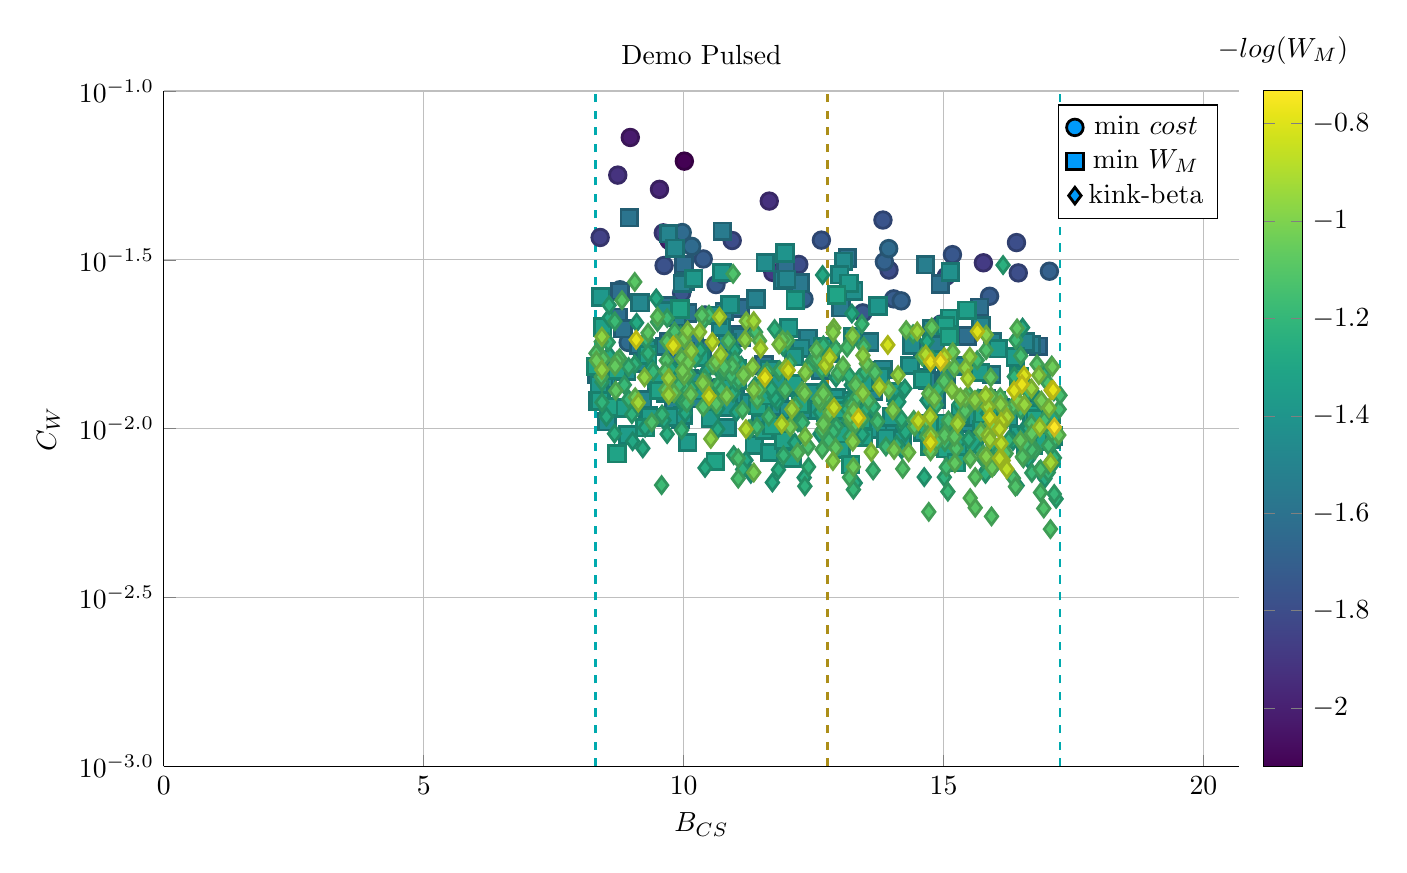
\begin{tikzpicture}[]
\begin{axis}[colorbar = {true}, height = {101.6mm}, ylabel = {${C}_{W}$}, title = {Demo Pulsed}, xmin = {0.0}, xmax = {20.686629468551892}, ymax = {0.1}, ymode = {log}, xlabel = {${B}_{CS}$}, {unbounded coords=jump, scaled x ticks = false, xticklabel style={rotate = 0}, xmajorgrids = true, xtick = {0.0,5.0,10.0,15.0,20.0}, xticklabels = {0,5,10,15,20}, xtick align = inside, axis lines* = left, scaled y ticks = false, yticklabel style={rotate = 0}, log basis y=10, ymajorgrids = true, ytick = {0.001,0.0031622776601683794,0.01,0.03162277660168379,0.1}, yticklabels = {$10^{-3.0}$,$10^{-2.5}$,$10^{-2.0}$,$10^{-1.5}$,$10^{-1.0}$}, ytick align = inside, axis lines* = left,     xshift = 0.0mm,
    yshift = 0.0mm,
    axis background/.style={fill={rgb,1:red,1.00000000;green,1.00000000;blue,1.00000000}}
, colormap={plots}{rgb=(0.26700400,0.00487400,0.32941500), rgb=(0.27794100,0.05632400,0.38119100), rgb=(0.28291000,0.10539300,0.42690200), rgb=(0.28229000,0.14591200,0.46151000), rgb=(0.27619400,0.19007400,0.49300100), rgb=(0.26514500,0.23295600,0.51659900), rgb=(0.25042500,0.27429000,0.53310300), rgb=(0.23360300,0.31382800,0.54391400), rgb=(0.21813000,0.34743200,0.55003800), rgb=(0.20123900,0.38367000,0.55429400), rgb=(0.18555600,0.41857000,0.55675300), rgb=(0.17117600,0.45253000,0.55796500), rgb=(0.15772900,0.48593200,0.55801300), rgb=(0.14618000,0.51541300,0.55682300), rgb=(0.13374300,0.54853500,0.55354100), rgb=(0.12346300,0.58168700,0.54744500), rgb=(0.11948300,0.61481700,0.53769200), rgb=(0.12632600,0.64410700,0.52531100), rgb=(0.15014800,0.67663100,0.50658900), rgb=(0.19109000,0.70836600,0.48228400), rgb=(0.24607000,0.73891000,0.45202400), rgb=(0.31192500,0.76782200,0.41558600), rgb=(0.37777900,0.79178100,0.37793900), rgb=(0.45867400,0.81636300,0.32972700), rgb=(0.54552400,0.83803900,0.27562600), rgb=(0.63690200,0.85654200,0.21662000), rgb=(0.73088900,0.87191600,0.15602900), rgb=(0.81457600,0.88339300,0.11034700), rgb=(0.90631100,0.89485500,0.09812500), rgb=(0.99324800,0.90615700,0.14393600)}, colorbar style={title=$-log( W_M )$}}, ymin = {0.001}, width = {152.4mm}]\addplot+[scatter, scatter src=explicit, only marks = {true}, color = {rgb,1:red,0.00000000;green,0.60560316;blue,0.97868012},
draw opacity=1,
line width=0,
solid,mark = *,
mark size = 3.0,
mark options = {
    color = {rgb,1:red,0.00000000;green,0.00000000;blue,0.00000000}, draw opacity = 1.0,
    fill = {rgb,1:red,0.00000000;green,0.60560316;blue,0.97868012}, fill opacity = 1,
    line width = 1,
    rotate = 0,
    solid
}] coordinates {
(10.014310061470209, 0.06197483174638786) [-2.119809409407475]
(8.974351824202143, 0.07282952610606806) [-2.022107373269494]
(9.720840649522977, 0.03609135913093006) [-1.9777667149411715]
(9.535747921961464, 0.051130362720294704) [-1.969913275543008]
(11.64719575750508, 0.047199699242522014) [-1.9276279243167613]
(8.733488072843636, 0.05634035623848662) [-1.9180907603558137]
(11.717151268119157, 0.0290156978870517) [-1.8866814459155106]
(15.76615725864231, 0.030992141550921816) [-1.8810042714594786]
(9.609717770109604, 0.03801538835634297) [-1.861231108978198]
(8.394527886005427, 0.03683114347875789) [-1.8558362580925096]
(15.053294230728687, 0.028291519575269056) [-1.811508198071671]
(10.934532396569558, 0.03607745072820276) [-1.8048956433290855]
(12.215380678409446, 0.030644555029908985) [-1.797922304180305]
(13.950900000393457, 0.02949537628440487) [-1.7974494679074275]
(16.437201647022366, 0.028933124859920306) [-1.7961193741663348]
(16.40261361811642, 0.03557653455378664) [-1.7922955251500743]
(9.624471357573801, 0.030417392770278703) [-1.7763653379983415]
(13.834221351663881, 0.04147970255534964) [-1.762574168304495]
(9.962006621581514, 0.025210912703269035) [-1.7524000959584443]
(12.65031002841598, 0.036173737778618126) [-1.7467043012053995]
(15.171180859324355, 0.032766263996239824) [-1.7445197156480476]
(13.447185867051214, 0.02202338694073385) [-1.7362913649987812]
(10.622905984575329, 0.026714074548194577) [-1.7340594740544224]
(9.687508349386887, 0.022713661122324157) [-1.7289223235866222]
(15.885358349462447, 0.02466928657304406) [-1.719614121069955]
(14.041145822343132, 0.024233508820652228) [-1.7167136137505041]
(10.377907964259716, 0.03181143352229567) [-1.7154437116459917]
(10.753780577931199, 0.028622291298276443) [-1.7060722509483957]
(17.03614113083419, 0.02926238447048653) [-1.6937830944780397]
(13.861622812084057, 0.03120868171359675) [-1.6889812321302553]
(14.184282250063832, 0.023905595143656186) [-1.686209077026567]
(12.315442430684204, 0.024204963735087338) [-1.6786883535604935]
(14.950434999553853, 0.020413682949498045) [-1.6734478593396724]
(10.4122328117203, 0.02171708878277083) [-1.650681965327452]
(8.776130848827346, 0.025789595420542006) [-1.6458495153344535]
(13.944616671700327, 0.034141771708853026) [-1.6412636709027566]
(9.972964073735131, 0.03809649700399676) [-1.6393314314904326]
(10.155668028711606, 0.0346599142742729) [-1.6390302509540549]
(8.93332912842768, 0.018002375584230325) [-1.6381696948341165]
};
\addlegendentry{min $cost$}
\addlegendentry{min $W_M$}
\addlegendentry{kink-beta}
\addplot+[scatter, scatter src=explicit, only marks = {true}, color = {rgb,1:red,0.00000000;green,0.60560316;blue,0.97868012},
draw opacity=1,
line width=0,
solid,mark = square*,
mark size = 3.0,
mark options = {
    color = {rgb,1:red,0.00000000;green,0.00000000;blue,0.00000000}, draw opacity = 1.0,
    fill = {rgb,1:red,0.00000000;green,0.60560316;blue,0.97868012}, fill opacity = 1,
    line width = 1,
    rotate = 0,
    solid
}] coordinates {
(16.82228492576424, 0.017540808339758972) [-1.6348798048481208]
(11.091923619988552, 0.022785258097976623) [-1.6277277898588538]
(10.00476818341642, 0.030625514244526048) [-1.627684330571819]
(8.777176250808912, 0.025489957683783454) [-1.6248467182009472]
(10.991846079958428, 0.0189830433690413) [-1.62256122166559]
(15.458683088869776, 0.018838350678554387) [-1.6197529434592726]
(11.964070298839442, 0.030553347689269015) [-1.619473374550493]
(8.73450389120548, 0.0213568595963161) [-1.6190205769362032]
(14.592694375647465, 0.017173711360022336) [-1.617478678707941]
(15.693294727899161, 0.022891816741403965) [-1.6135161817566324]
(14.936949374526826, 0.026834336105762403) [-1.6079101518459553]
(8.83184401567771, 0.01976733422078956) [-1.6005797137016178]
(9.72150547040655, 0.01811055755791537) [-1.5991182248913247]
(10.078203743630864, 0.02202289176749285) [-1.595836360479248]
(8.954209756242996, 0.042161103004000076) [-1.589397412964098]
(9.673607099925281, 0.0231728109038665) [-1.589205111302375]
(11.543935756448146, 0.015450272567257462) [-1.5875377953010883]
(13.151617966814817, 0.0319953061173649) [-1.5845809864087244]
(9.781030534247606, 0.016164039710660088) [-1.5775674018565111]
(9.303102469493684, 0.016693759971981265) [-1.5713155071601692]
(10.359872502096119, 0.01726409176752251) [-1.5652457853616617]
(12.237632180874417, 0.02698353416604086) [-1.5643952661253622]
(9.144801617136775, 0.01769761001811183) [-1.5595601870169422]
(13.029635600163276, 0.02281153437267921) [-1.552568848396255]
(10.7422001331706, 0.038423068705951594) [-1.5520441226990631]
(10.780757247562724, 0.022224095489930037) [-1.544925041354305]
(10.200715682654506, 0.01841847429182733) [-1.5430023738862098]
(15.017329028039686, 0.019477644457703495) [-1.5396243114452017]
(8.334002624663501, 0.01449908817629988) [-1.538692217528126]
(10.555701885198872, 0.013092644307368572) [-1.5373740781698282]
(14.65414605441725, 0.030574977212997605) [-1.5350312948909135]
(14.660222353908768, 0.014205258889817484) [-1.5317433014682034]
(11.106568774256633, 0.018689708848548738) [-1.5311850486265117]
(14.689056206740792, 0.01387590038164943) [-1.5287451237254033]
(9.473959265162193, 0.013905952265261586) [-1.526526816139614]
(10.035372496295135, 0.027241135712482305) [-1.519178921439465]
(10.039027121575653, 0.016910779414334946) [-1.517891032933806]
(11.39227618908412, 0.024191852864153648) [-1.5130165343032327]
(16.679321236285688, 0.01773125993862434) [-1.5126055054907948]
(11.906042879430306, 0.027530426264504002) [-1.5122759735909235]
(13.642157714321597, 0.014899481481132758) [-1.5121531835443067]
(14.850116736119897, 0.01778122202031051) [-1.5121518481580156]
(12.392450828732116, 0.01852162588841651) [-1.509963665969106]
(11.613487062213123, 0.013259386458548635) [-1.5098191352881933]
(13.579000388347866, 0.018078145365757758) [-1.5094600237705913]
(9.867201865947047, 0.02134336001409843) [-1.5091677016781566]
(9.643385161260726, 0.017507453096671365) [-1.505813383704145]
(9.97586799244543, 0.026909424888676328) [-1.5035180904231982]
(15.94212072748298, 0.018116695499993292) [-1.4998070828001184]
(10.309179324950696, 0.01226652304303364) [-1.4993412700061268]
(12.638042249859588, 0.014898889997617197) [-1.4970388348465338]
(15.055675671525783, 0.014279317114283529) [-1.4968151314329754]
(9.710222870228767, 0.03778412752723575) [-1.4959262215207656]
(9.813107231605422, 0.012007443130458324) [-1.495878750102406]
(9.685925965003944, 0.014131383104205364) [-1.4911760171512294]
(11.714098265194735, 0.013847785437885679) [-1.4909012021072667]
(10.994639674638705, 0.013113327535403696) [-1.4904727997922445]
(15.819989093254375, 0.012253217681920671) [-1.4902975254497872]
(15.716610680795545, 0.020179920200301855) [-1.4899596862430686]
(15.924465247564154, 0.014465480638895564) [-1.484315053758591]
(8.416214966248592, 0.012974868808400592) [-1.4832272441818983]
(11.981607928881237, 0.02767164571202513) [-1.481908947186888]
(11.711067257135763, 0.012700241486954703) [-1.481610811848838]
(16.57758432667383, 0.018066556725317685) [-1.4808315890609627]
(9.214130290028436, 0.012152582495637852) [-1.4803924190961808]
(9.16252648162826, 0.023591043628319753) [-1.4777813991456452]
(13.841485576616298, 0.014987126189756067) [-1.476226145125234]
(14.86036210936636, 0.012179602718049342) [-1.476103765156545]
(14.771702357628312, 0.0198044997246676) [-1.4759532635696884]
(11.751019990155784, 0.011854698849849837) [-1.4744693843941874]
(9.214130290028436, 0.015665176708494814) [-1.4721189566530006]
(13.644386027863185, 0.012892988065699775) [-1.4694765884704042]
(12.673551051198132, 0.011723605612914264) [-1.4684762544315009]
(16.7437460203336, 0.01146148363735155) [-1.4673712598422484]
(10.114476569413018, 0.01403086783418577) [-1.4665127712450712]
(9.836829838606402, 0.03422172209265897) [-1.466465342676487]
(15.478205114940627, 0.011814056076879775) [-1.4656409913573911]
(10.852786830516008, 0.01666169164744686) [-1.4607639902508311]
(12.451557765219139, 0.011797068547740396) [-1.454804800167485]
(14.385054216404878, 0.017714850999176746) [-1.454016548396377]
(12.250517419581046, 0.01730924236440855) [-1.449126660054787]
(15.399238782030915, 0.015350811156516968) [-1.4450317564339483]
(15.323964495196108, 0.010700521525178483) [-1.4442476160174416]
(10.840350242413816, 0.017999193081243068) [-1.4428695943470562]
(13.07657469813823, 0.03129913412451443) [-1.4416527786165851]
(11.571153759168391, 0.030992801350489627) [-1.4412978501823663]
(10.159175807081688, 0.013876797144792313) [-1.4410674847520173]
(14.65870048492913, 0.0103371343106061) [-1.4407593364531412]
(9.64911680597678, 0.022291694526716137) [-1.4382523340904476]
(11.824660750219888, 0.011033535668865918) [-1.4374618391296154]
(16.090603216081107, 0.011578760205733224) [-1.437309497392895]
(8.526794202732354, 0.014225493350487712) [-1.437004502630189]
(11.836002040544534, 0.011662685993065088) [-1.4369516286418977]
(15.4684670810238, 0.010363517857158673) [-1.4359296968945898]
(11.551257449345478, 0.012593943496598788) [-1.4348111698815942]
(8.523380131000312, 0.010486068251726523) [-1.4347403934029699]
(12.329900028804074, 0.011351647420548932) [-1.432162507533083]
(13.236600826453692, 0.010703895251080882) [-1.4298959659652046]
(16.83282359352303, 0.010279170294604838) [-1.429141349371285]
(13.269307990860742, 0.025557043779995653) [-1.4288294492620477]
(10.717109038917776, 0.019981046165081038) [-1.4275892047251812]
(8.463326863230373, 0.014011150106021747) [-1.42664672926539]
(9.292495803166666, 0.017276630179413652) [-1.4239039330716527]
(12.01294221545527, 0.01135063897630595) [-1.4237047673472223]
(10.642574031409726, 0.021651736693319764) [-1.4220880228019461]
(15.130371291452986, 0.029124606257697153) [-1.4214589216983458]
(13.449121379363364, 0.010524080735331771) [-1.4192750546166355]
(10.598536227766495, 0.012152497168515361) [-1.4188846212567885]
(9.94286005160173, 0.010654264771940928) [-1.418142111238707]
(8.354283940274188, 0.012093014306414056) [-1.4175771687309422]
(11.490654672775422, 0.010307835186267926) [-1.4166515403180218]
(13.927755889931667, 0.009802839106844477) [-1.4151591623618127]
(12.896498202515414, 0.012089411129630757) [-1.415086999740124]
(12.813665090982388, 0.016771907819218872) [-1.4150518254702726]
(8.905845640255238, 0.01479570625667246) [-1.412750376425469]
(13.001742838316293, 0.02858609969916251) [-1.4118418857799215]
(14.802174067631956, 0.009976658176736495) [-1.411745253778192]
(11.208912070421409, 0.011899859669740264) [-1.4101129990450592]
(12.913000276070724, 0.010975696046095008) [-1.4098064292280077]
(10.84161307277213, 0.010078193568331789) [-1.4071217370506766]
(10.952245284131447, 0.012567870805096065) [-1.4069653518342513]
(15.465550241086678, 0.010809590548122633) [-1.4053188021751997]
(11.888760566686239, 0.013228123351848638) [-1.4040831795581317]
(9.656977955682123, 0.012756284815624411) [-1.403783408224447]
(12.357969070297273, 0.011849909135487101) [-1.4034059706684434]
(14.354705949019486, 0.015391572104901911) [-1.4031334212883295]
(15.759091197715701, 0.011370525417095621) [-1.4027031557706915]
(15.93492167661274, 0.010883116023126084) [-1.4023409214316394]
(11.950351989604266, 0.03314304390232683) [-1.4018234466267534]
(9.31395933016945, 0.010943279854872806) [-1.4001967788421508]
(12.501198744996175, 0.012776602146795163) [-1.3983213447403338]
(16.691702745627914, 0.011065372696240975) [-1.3946316971345938]
(12.793680134727829, 0.009697674748088487) [-1.393981306323598]
(12.945145532203291, 0.012316212001497684) [-1.3939743444895971]
(10.895241072523511, 0.023293627402023516) [-1.3938659098694006]
(10.624418674781085, 0.012799262525216688) [-1.3934317035795]
(13.736998867652822, 0.02306752096780418) [-1.3919378361313393]
(10.86446674023058, 0.011575943181240602) [-1.3913501343623875]
(9.989604552735361, 0.010938935413839007) [-1.3899986150261634]
(11.65036209258509, 0.014916276865219583) [-1.3888953225499234]
(16.253794354777128, 0.010811642128190005) [-1.3883849558567678]
(13.237511348589962, 0.012086573842968483) [-1.3880683151937296]
(13.3098445206835, 0.00974951527611275) [-1.3879257169733152]
(13.250391582535599, 0.01875474559032549) [-1.387200255154835]
(10.737511566041665, 0.028992717747430105) [-1.3869139374162498]
(13.77662330230216, 0.014275341697562267) [-1.385982080919773]
(15.808216920395289, 0.009658736241223327) [-1.385951966541943]
(13.731078012406766, 0.009979205376142167) [-1.384341496966052]
(14.597629824496682, 0.009781750047901397) [-1.3836628266676982]
(10.193517952021443, 0.027837899406166513) [-1.383138617240496]
(11.85882016006122, 0.013692957043690078) [-1.3831333668949872]
(15.990533435344123, 0.012055028195149642) [-1.3823755173012382]
(8.403151177328072, 0.02457168150365556) [-1.381386436684111]
(8.38045546510813, 0.013467436970042478) [-1.381013926041926]
(12.120810510968868, 0.01632900764605371) [-1.3807582017142732]
(10.203415923531363, 0.016233342907168043) [-1.3795912650626003]
(12.022820996636117, 0.019856726760879642) [-1.3784744825946547]
(14.941654987190931, 0.009937020814786353) [-1.3784050115817357]
(10.30431640058217, 0.012947457233964572) [-1.3727350903904059]
(13.179314023604123, 0.02692798924274793) [-1.3726382795387042]
(11.360939883051167, 0.00894061047284123) [-1.3726183217257064]
(9.712824116971364, 0.01083618948017438) [-1.370506635821487]
(13.999353699862713, 0.010820381028973857) [-1.3702834841058706]
(11.029519708444795, 0.01507474130083674) [-1.3699905172740252]
(14.790388677939154, 0.016024901755414496) [-1.3694510931398833]
(14.2011289491935, 0.009286958803152093) [-1.3690194932725448]
(16.05186059099198, 0.01725165686414962) [-1.3685993689556193]
(10.079551280694128, 0.009100422809121853) [-1.3680782620249432]
(13.891099279827657, 0.009358898748733285) [-1.3659937757563743]
(10.51469839684549, 0.010741593794976297) [-1.3655266043175585]
(16.97679926285361, 0.00935804014953258) [-1.365489135635999]
(16.382025622806193, 0.01631624677926724) [-1.365314944668722]
(12.601871821561915, 0.011316654652064283) [-1.3620488306806053]
(9.342717740515683, 0.010811158792461435) [-1.3600883836878876]
(15.699013106793902, 0.014663988794896813) [-1.3569999482959285]
(17.08124053314885, 0.009327975573933072) [-1.3565369493574833]
(8.929819918270683, 0.009591330831744169) [-1.3564434514013937]
(17.107810871536294, 0.009510520762087537) [-1.355670949654743]
(15.272532347809275, 0.008600603815848054) [-1.3550689180362785]
(15.113272758939148, 0.0212306523206366) [-1.3545717493575382]
(12.758115395547385, 0.011027495783414606) [-1.3536406793714741]
(12.146510141523258, 0.02403578580290836) [-1.3522480304376618]
(9.802895887224908, 0.01277987363566607) [-1.351683168790268]
(12.731812711004267, 0.011181317227288103) [-1.3509416538039447]
(14.597629824496682, 0.013988110662625983) [-1.350917699634303]
(12.937418062164188, 0.011706003302806382) [-1.3498675794038522]
(12.680634700802198, 0.01744787935363008) [-1.3480954361555229]
(16.547895069902516, 0.009513333911267541) [-1.3474307155472665]
(11.653216567545261, 0.008506399274340092) [-1.345835600508895]
(15.44880839508013, 0.022402494346273383) [-1.3441619287129023]
(11.525312140201327, 0.011568935524735228) [-1.343173024895477]
(11.552250427675727, 0.009888039453025594) [-1.3431102335422052]
(13.467268933575436, 0.013676025720795522) [-1.3418959513921676]
(15.323265928492141, 0.011055478792069253) [-1.3416390955818198]
(12.121641590617898, 0.013562184857025608) [-1.3412225668983788]
(11.024065356801717, 0.013928329166195007) [-1.3411223781363122]
(16.734724817567656, 0.008957609956171385) [-1.3409980727589041]
(16.769045540215842, 0.011061155580644737) [-1.3407774046291352]
(9.473959265162193, 0.014142372730384274) [-1.340736718067575]
(8.74505555084563, 0.014931289500105476) [-1.340172101894623]
(13.027598279499255, 0.008673821452175847) [-1.339371225527388]
(14.069726621490684, 0.012851757813003692) [-1.3355889626958743]
(16.45157670371507, 0.009585198585080813) [-1.3353537500446666]
(8.828372531773972, 0.011502571386254939) [-1.3352936153265889]
(15.043191855376238, 0.020177908654106694) [-1.3347167954999664]
(15.87555423129121, 0.010934192827515073) [-1.3333464153994234]
(14.74050555979749, 0.010187040046408826) [-1.3319467069356516]
(8.394635001603197, 0.012093243108414115) [-1.3317606682979195]
(15.737459460817936, 0.0099544891977854) [-1.330878268232421]
(16.577004376563345, 0.00892167491417854) [-1.329838199225075]
(8.442119987401155, 0.020024514359414238) [-1.3275817805394716]
(15.03780769292473, 0.010377685225384297) [-1.3271981479523673]
(11.923687420170552, 0.00923521460571462) [-1.3257753666633474]
(9.311244990438865, 0.016536435428404248) [-1.324805801675252]
(12.08205721926947, 0.008177838551829547) [-1.3236480395933032]
(10.75205842676705, 0.01320289357034274) [-1.3223872875360454]
(13.461717625918478, 0.009416665871049234) [-1.320790714548859]
(9.519960674752117, 0.012966997564871513) [-1.3198610091294973]
(8.715815013641683, 0.014941915896507264) [-1.3173999901029887]
(9.815532890733682, 0.014705731648914599) [-1.3172398911361078]
(15.109422453252336, 0.018745840734049092) [-1.3155841266914403]
(14.740296253242736, 0.008883845818604448) [-1.3144429555765318]
(10.31653236444549, 0.016334708642476756) [-1.3140984246311314]
(10.60954534582113, 0.007999169369094802) [-1.3136141988883636]
(13.432319600929263, 0.010593671042148305) [-1.3130409307938926]
(11.42823386655995, 0.011696426000066894) [-1.312883593567563]
(8.719380611168567, 0.008437215022084032) [-1.3113636666391015]
(11.696923395666094, 0.010210442889078589) [-1.3110543205827916]
(8.560854879579562, 0.01161135507437133) [-1.3101666476591896]
(16.764368284085073, 0.010715857251244127) [-1.3094281744638252]
(15.192999611497397, 0.007935513211517508) [-1.3092819198295769]
(8.315725665672304, 0.01527961135499392) [-1.3091789421820008]
(15.043366759433116, 0.008718673720708605) [-1.308657609117127]
(16.021238035205084, 0.012115862676003172) [-1.30815684782275]
(11.593073557294613, 0.012528702800938256) [-1.3073192126014976]
(15.192999611497397, 0.009466859805614364) [-1.306104667504652]
(12.945145532203291, 0.024862203238592617) [-1.3061029424340123]
(9.927382980222017, 0.022588731344076834) [-1.3059932173472433]
(9.256949266351661, 0.010067194372351543) [-1.3053424100316993]
(16.82199006964077, 0.009194414774426339) [-1.3048906180553326]
(16.45157670371507, 0.014224364223609164) [-1.3043596581137094]
(13.051048964875424, 0.00966642720928779) [-1.304157201921016]
(15.244913096432274, 0.007934056288357859) [-1.3040523349428945]
(12.245141259071001, 0.011830250137913223) [-1.3039439069452712]
(16.026769470614276, 0.008152912507864905) [-1.3022467953572583]
(13.051048964875424, 0.011323662495891916) [-1.3012176243848619]
(15.591542980066137, 0.009074217857747638) [-1.3011866801418175]
(17.068912884842916, 0.011011974496683653) [-1.3004916659282275]
(13.212953491584514, 0.007824745570931163) [-1.3001880033121107]
(15.749170807222828, 0.011078402389842862) [-1.2993649239636758]
};
\addlegendentry{min $cost$}
\addlegendentry{min $W_M$}
\addlegendentry{kink-beta}
\addplot+[scatter, scatter src=explicit, only marks = {true}, color = {rgb,1:red,0.00000000;green,0.60560316;blue,0.97868012},
draw opacity=1,
line width=0,
solid,mark = diamond*,
mark size = 3.0,
mark options = {
    color = {rgb,1:red,0.00000000;green,0.00000000;blue,0.00000000}, draw opacity = 1.0,
    fill = {rgb,1:red,0.00000000;green,0.60560316;blue,0.97868012}, fill opacity = 1,
    line width = 1,
    rotate = 0,
    solid
}] coordinates {
(14.682772921069034, 0.012133883145293747) [-1.2971735267311564]
(16.555137236197424, 0.008497507185750146) [-1.2963451470925318]
(13.179991464330723, 0.011968595839803002) [-1.2939289874566402]
(15.888696111510232, 0.008051203599652048) [-1.2928570974581939]
(16.651463466334494, 0.009198462479520332) [-1.2926592596370523]
(16.555137236197424, 0.009976448637174172) [-1.2918359622137705]
(11.015371517921224, 0.011200517330116096) [-1.2901565279273088]
(10.43448368514836, 0.014778677283745992) [-1.2885231243501492]
(12.62262254375668, 0.009645840422057206) [-1.2873870680148987]
(11.10781988195937, 0.015368153744705897) [-1.2867189599495152]
(16.82199006964077, 0.012200186404574626) [-1.2866608738447551]
(15.327000264646497, 0.009314200607444962) [-1.2862989627940875]
(11.293041040527157, 0.007351086075188858) [-1.2856479743658245]
(12.62262254375668, 0.011184811263709776) [-1.283461572944208]
(12.673551051198132, 0.028511756618296732) [-1.282628142229196]
(9.018740260054527, 0.0091809969411667) [-1.282318795548118]
(9.378254722237372, 0.015147418693115068) [-1.2809419797501462]
(16.67207354194001, 0.009441743395354373) [-1.2802239523296417]
(14.221898977802105, 0.010115067051441084) [-1.279661807174519]
(14.193898850417899, 0.008682653521467484) [-1.2793586996677089]
(16.335988065907316, 0.00919694313697991) [-1.279241431080542]
(11.199032883922865, 0.008062649665833432) [-1.2791738597664242]
(8.565625511562189, 0.016537125137685977) [-1.2777724695025643]
(9.473959265162193, 0.024311609583825906) [-1.2776560252665474]
(15.820537682670786, 0.007543708329813699) [-1.2776226586446298]
(13.223938971427943, 0.013472425466080754) [-1.2772080908839465]
(9.6224419440208, 0.010591022499429533) [-1.2768888641183538]
(9.259381405997736, 0.010068814155906535) [-1.2749252706301877]
(10.02950074316046, 0.011122028940902477) [-1.27405635520294]
(9.096410727756737, 0.020592443763116842) [-1.273999627133777]
(11.250274296159523, 0.009932693135460512) [-1.2739263340884897]
(16.651463466334494, 0.013177764718534145) [-1.273686836355838]
(13.236600826453692, 0.021930543698997433) [-1.272060671091855]
(10.988390518242154, 0.01703366147805158) [-1.2717552020206426]
(12.689774417510133, 0.013199694993892157) [-1.2715552113887816]
(14.682772921069034, 0.018137179053328113) [-1.2711256143593725]
(12.138235311074201, 0.009089213335736035) [-1.2706918059143955]
(16.51983071545539, 0.019922160606497104) [-1.270659241243097]
(13.440224729488612, 0.009612072783370788) [-1.2706266042708976]
(14.056438663449487, 0.011815687417752718) [-1.2699973230973551]
(16.632293213183402, 0.008127375094877596) [-1.2694883213650459]
(15.843105813982604, 0.011108460101523684) [-1.269469949244091]
(14.139022745673238, 0.01200413289507089) [-1.2693810054133523]
(8.565625511562189, 0.021322131632939743) [-1.2685038799823198]
(9.215460716271485, 0.008746022086925008) [-1.268011220133286]
(11.79925508433291, 0.012071261699451271) [-1.2676767161765092]
(9.767648689516832, 0.015027760071695463) [-1.2672360183442966]
(9.905927226247794, 0.012386782250268949) [-1.2670329245716005]
(10.65725161660864, 0.00997135774995843) [-1.266521603924258]
(10.055681915858392, 0.014743359804979298) [-1.265829536383991]
(12.138235311074201, 0.011015221663609409) [-1.2655850749955841]
(14.267102900143742, 0.009754591610171831) [-1.2651606387913807]
(16.568716501758974, 0.008391084675782472) [-1.2650267302153226]
(10.65725161660864, 0.011459660264397842) [-1.2643165163116283]
(14.25689481086506, 0.01314380020899071) [-1.2638630587832318]
(16.632293213183402, 0.0100188505842072) [-1.263682663264664]
(11.707584495779955, 0.006930908540990179) [-1.2635507051033026]
(10.412391370371594, 0.007655768190498255) [-1.2630930817893484]
(15.707955638238712, 0.008595102325139414) [-1.2620028969039807]
(15.941689167985352, 0.008993269936185943) [-1.2617711256664215]
(11.618449420251658, 0.013435175267701598) [-1.2607622270815175]
(11.906052951232901, 0.010399130132164968) [-1.2599969566754825]
(13.422765787398976, 0.011066872440514844) [-1.2580199333772297]
(12.931935336308614, 0.014164623239439114) [-1.257674742909116]
(16.4155019400067, 0.006784814729690784) [-1.256920205986828]
(8.514832197721942, 0.010847484174753686) [-1.2558826127376497]
(9.960307841751561, 0.012006910499828622) [-1.2545784323742915]
(11.751019990155784, 0.012367303307791636) [-1.2541769145790829]
(13.300908706718086, 0.006909773766752695) [-1.2538081670568602]
(16.949195577210475, 0.007118806510545466) [-1.2537331036632384]
(12.318542112721676, 0.007163920014099904) [-1.2523947287534352]
(9.960307841751561, 0.01409766195530951) [-1.252161894882265]
(14.628561786858135, 0.007191926525759095) [-1.2517841257242934]
(15.90674460516089, 0.010140660180167243) [-1.2510148685101052]
(12.87923916901645, 0.009947685467565285) [-1.2503817284236358]
(11.824591933033416, 0.00755783116205777) [-1.2500618007814928]
(10.31927503264005, 0.01705584468677382) [-1.249408930050928]
(15.977434181824485, 0.007782048369656626) [-1.248434923528094]
(9.683456615169344, 0.009638865392082259) [-1.246475793101881]
(8.671623187801623, 0.009668090359024908) [-1.2453083223674235]
(15.299311115315916, 0.01181801423349667) [-1.2430271033455136]
(10.952245284131447, 0.012765537294567253) [-1.2425009663963265]
(13.37865937666007, 0.014096920088512531) [-1.2420036959161107]
(11.040941770182885, 0.014638041989732616) [-1.2406291651922927]
(13.488578301097156, 0.011330221246013529) [-1.2404081246835275]
(14.628561786858135, 0.009882346466549934) [-1.2402721066912186]
(16.145232878087864, 0.030517882462548936) [-1.2399829928026451]
(9.943887569980818, 0.018855374361929193) [-1.2398403601837327]
(11.689159647203805, 0.013105067185166342) [-1.2382227382575577]
(8.567148568313412, 0.023206171452307512) [-1.2372685823332665]
(11.915585134033648, 0.01748239328622686) [-1.2369979991721363]
(12.198645212509877, 0.010436966421480154) [-1.2364971528125899]
(15.48431465614079, 0.00929031971105747) [-1.235918342000411]
(9.047649397424134, 0.01224311754662533) [-1.235332112263366]
(11.376707871371156, 0.013377000135851953) [-1.235230354209212]
(16.840748740961537, 0.00752176857171885) [-1.2348662947331168]
(11.136175174634447, 0.007577390318458053) [-1.2331237451825037]
(14.097655097755435, 0.008954934736687754) [-1.2314216648450123]
(15.807042377277515, 0.007348723496235854) [-1.2276908244938955]
(12.33207356829479, 0.00675688814735783) [-1.2234874983546444]
(10.222252038737434, 0.01611655322423877) [-1.2224132121245386]
(16.251358747135995, 0.009234491873309686) [-1.2212129344183997]
(12.723834447815875, 0.012691970303684906) [-1.221000044288545]
(9.004625505986517, 0.011032294768272291) [-1.2201668573985105]
(10.678976402706837, 0.014875616723151944) [-1.2200113852982524]
(13.05961095465478, 0.014755597501979523) [-1.2200110437170943]
(9.058040813922531, 0.015480160187022769) [-1.2199386530853975]
(11.751019990155784, 0.019725018407248666) [-1.2192027637421239]
(15.662199761760458, 0.01227428321856098) [-1.218844626416703]
(11.002753780917594, 0.013727476887235461) [-1.2187513907488479]
(15.014532020154196, 0.007184219051293641) [-1.2182120816961266]
(13.148749979709805, 0.011425165896800414) [-1.2178523450390264]
(9.316969297353253, 0.01671459075301228) [-1.217564445140848]
(10.154270603961049, 0.01316079396243774) [-1.2148287908302686]
(14.19279870188835, 0.010653867811546877) [-1.2144650329368094]
(17.165092473837838, 0.006198307301760009) [-1.2142295699793069]
(15.014532020154196, 0.009725241928162248) [-1.2114971471794018]
(10.964602796324286, 0.00834877000609595) [-1.2110590840755884]
(12.25459113238908, 0.010394495894857034) [-1.210956786812969]
(13.649393629962841, 0.01160689504064373) [-1.210625479626572]
(12.40274647042282, 0.007709496307162327) [-1.210548450407708]
(8.42941267292461, 0.01196700634860152) [-1.2101072964851303]
(16.360665913232772, 0.014267222031421351) [-1.2097043828037173]
(12.688686022519612, 0.017649120721508472) [-1.2090548152300868]
(17.101933862003563, 0.00786922573538261) [-1.2089432452477198]
(13.212953491584514, 0.018050177035811292) [-1.2088567702310062]
(8.42941267292461, 0.01374396978202603) [-1.208355792529063]
(15.807042377277515, 0.012119563498851512) [-1.2079597098695036]
(11.826932290539112, 0.01476620759208673) [-1.2069143247822283]
(16.937250320827843, 0.014425121215984256) [-1.2060355587049236]
(16.56929514507332, 0.008818373193963157) [-1.2051439881244612]
(13.181524156722897, 0.014347196234709005) [-1.2048202874468241]
(14.89986738586979, 0.013090961135950088) [-1.20412102013171]
(17.131922906542755, 0.008195788944222735) [-1.2006084749599055]
(9.584782689444218, 0.011017845567179161) [-1.1997509076464346]
(13.490860552242111, 0.01471498897475931) [-1.1989561148134826]
(13.176473234117513, 0.010576750792174504) [-1.1977552093777106]
(10.988245035999599, 0.015955953274896677) [-1.1973464324024234]
(15.038409502255757, 0.014024797653122234) [-1.1952843257986516]
(9.961762717388044, 0.009913142251828634) [-1.194608172565493]
(8.942050925672243, 0.012231614304186931) [-1.1943983553124515]
(17.120985015074893, 0.012895825589119291) [-1.1943709063726027]
(11.920999462954518, 0.008341248647504823) [-1.193465520169887]
(17.014436731421398, 0.007422215660710276) [-1.1934529196767811]
(8.548963250971841, 0.018029259293378272) [-1.1932608414538086]
(9.416726619046099, 0.01475503745943627) [-1.1930245850534404]
(12.4394525554187, 0.01559839957452813) [-1.19275308105931]
(13.265902368751764, 0.006601321305241876) [-1.1925650410586528]
(16.6299411017185, 0.012849471675853265) [-1.1916847830033912]
(17.129202501787184, 0.006406786662781295) [-1.1906829642457115]
(8.942050925672243, 0.015231829402577652) [-1.1905171502567853]
(9.27906715150467, 0.018424630927819426) [-1.1868792227109848]
(10.021428108030735, 0.012087057868798792) [-1.1860893620286155]
(14.77757376918867, 0.016048418150957987) [-1.1858875370196502]
(10.454025691365954, 0.011972397837837176) [-1.1854558952607928]
(8.86037108397972, 0.013483711604703155) [-1.1848213366225184]
(14.860405552114257, 0.011761816070313931) [-1.1847475832442582]
(16.697734081097174, 0.007399398212169979) [-1.1837916630431773]
(12.287202704452202, 0.010413257435217902) [-1.1834175022102877]
(13.199631705820181, 0.009470444499328991) [-1.1831305353511883]
(12.04002156741698, 0.015647472969860403) [-1.1828511911535706]
(13.429268295632518, 0.020407456319850734) [-1.181840770808167]
(15.083042498987238, 0.006510208938595967) [-1.1814651012301538]
(12.93585934283502, 0.010147346100150811) [-1.1809344434678004]
(15.08903520717264, 0.010306295906351105) [-1.1788261142099545]
(12.874280008939282, 0.00975845363999315) [-1.1783873972417303]
(9.683456615169344, 0.021255557406142055) [-1.1773891261145735]
(13.645133488301468, 0.007530050850229014) [-1.1772489110999693]
(13.89170225379231, 0.008856286376022381) [-1.1771937197283155]
(8.67737182027737, 0.02079595788529988) [-1.1768483795316644]
(10.771643002371896, 0.01477464262853022) [-1.1754670828809672]
(10.657856383500425, 0.013447350775475101) [-1.1748259721272571]
(16.06471023259536, 0.008533818365309384) [-1.1743579362801864]
(17.1316836490387, 0.00926629982316415) [-1.1731424023398116]
(15.026041337358697, 0.009127162071787865) [-1.1728411497954707]
(9.576609781620636, 0.006808109484569134) [-1.172547785671985]
(11.279560489781714, 0.009974514104150454) [-1.171293732602548]
(11.847882069406987, 0.014894587057756483) [-1.1706435645347975]
(12.662794223849232, 0.014934801738779929) [-1.1704804143126533]
(16.3897848180077, 0.018312728464608994) [-1.1694340492000508]
(10.730031930410188, 0.013038425730797958) [-1.1664836698360914]
(16.484580953127526, 0.011350876468389677) [-1.166021933665907]
(10.407320998161198, 0.014066615859663486) [-1.1653547583030963]
(11.639069714872814, 0.01085952514652926) [-1.1637013339225117]
(10.006343137186239, 0.013377410828925157) [-1.1629231949973953]
(11.059345377913772, 0.013971916288186385) [-1.1625677338545028]
(12.40274647042282, 0.01498663044146402) [-1.1615160270969884]
(10.06408250853542, 0.011904820041118874) [-1.1613847421954753]
(9.902431073117565, 0.013362365525672213) [-1.161380763910868]
(14.413146086048558, 0.019049310191542535) [-1.1612715538980343]
(11.410705501319088, 0.010122141818818486) [-1.1608808882180581]
(16.090315471306553, 0.011629604231527799) [-1.1602959592128257]
(16.535372216388026, 0.008169777889897055) [-1.1601187846950554]
(16.106899256187383, 0.00834966465898116) [-1.1597072302883453]
(10.09639230576176, 0.014522157751088465) [-1.1596295654776811]
(10.914467071854592, 0.014324434384547807) [-1.1584930595938716]
(15.760042238713773, 0.008145962416336265) [-1.1583013384515075]
(16.758572280032737, 0.008646050418225202) [-1.1578217536561153]
(17.018646604266053, 0.007816314398845932) [-1.1564044749404534]
(12.796253779221516, 0.009241849076330648) [-1.1562110876559482]
(15.052414924338043, 0.007695271029389756) [-1.1558406723410226]
(15.647072980506872, 0.015939165384127457) [-1.1551976368183803]
(13.731078012406766, 0.010505037613581628) [-1.1547723960660046]
(12.92675278881294, 0.01720072822154318) [-1.1547042721803664]
(17.018646604266053, 0.008918107308299703) [-1.1544971334332936]
(16.253794354777128, 0.011156083675037292) [-1.1514583143146417]
(10.39603038372212, 0.021035989307587558) [-1.150606587165903]
(13.463766396551701, 0.017520815218592205) [-1.1497568820513546]
(11.384733765960362, 0.019315926185319167) [-1.1488471764736738]
(16.484580953127526, 0.016442878704583205) [-1.14854127278881]
(11.604112098987112, 0.0147653907680726) [-1.1481443824350337]
(9.497296911957019, 0.02069244645197561) [-1.1475056240535222]
(10.488224449472721, 0.021750535713550727) [-1.147314943378139]
(17.223162892419708, 0.011413531346774588) [-1.1452162507505037]
(12.150894786402327, 0.011657490769208391) [-1.1440985305669964]
(16.68930628775202, 0.008671087589979474) [-1.143892607737901]
(16.569886893433157, 0.008990361186615302) [-1.1425154271844815]
(17.23885789045991, 0.012558201977665608) [-1.1419282223298928]
(16.936340179186345, 0.010576229210216307) [-1.1414111342865825]
(14.737732430469173, 0.010807673225691976) [-1.1409606377195203]
(16.68930628775202, 0.010350872866134037) [-1.140632380055554]
(13.442192340718403, 0.010685556097930418) [-1.1405059694207205]
(16.212323704366778, 0.010680444710790922) [-1.1402761489506106]
(11.549625061051866, 0.01443507208815689) [-1.1390460916159142]
(16.86604828682311, 0.007579718089160525) [-1.1390342976608838]
(17.08124053314885, 0.009743368571375198) [-1.1383859727853913]
(15.465550241086678, 0.011556690979889052) [-1.1378233474839952]
(13.14480493296275, 0.01739508549026366) [-1.1377132966757475]
(13.247068833500391, 0.011726874929476301) [-1.1376503199229564]
(11.050777266016288, 0.007116540390245059) [-1.1370921105287648]
(17.00860271346254, 0.013630883580602493) [-1.136359546149739]
(12.74928812237468, 0.01526251681202216) [-1.1362968805162]
(9.828339372234877, 0.019391120833403556) [-1.1358988321292471]
(16.412079199162257, 0.011860427509089479) [-1.1358539207185072]
(11.050777266016288, 0.008170611753766615) [-1.1356493088623822]
(13.190058867236672, 0.007176648981252689) [-1.1354932328782563]
(16.343118613330425, 0.007134995489417047) [-1.1335001124055868]
(11.133919631731134, 0.011362840629455528) [-1.1323762690185122]
(12.973701334746814, 0.014605309967466338) [-1.1314565774222176]
(11.954226224374837, 0.013041177771875015) [-1.1310401855629826]
(16.86506841916708, 0.006470994712702174) [-1.130758874865596]
(13.342005434244879, 0.01241454353087534) [-1.1307392487451149]
(16.12398815332631, 0.011706749993287805) [-1.129690412643984]
(15.094274129902931, 0.01058602765458819) [-1.1289684185709847]
(12.56748354328549, 0.016110870179123358) [-1.128250192514324]
(13.554151997056962, 0.012109336313631335) [-1.1252475037678356]
(12.394305575398981, 0.008853551975990904) [-1.1245713568718563]
(12.666314398171494, 0.008673362533302236) [-1.1245104109679405]
(9.38696353728333, 0.010444270942938963) [-1.1242443075431308]
(12.666314398171494, 0.009907337069737673) [-1.1228938533825863]
(8.76764666380086, 0.01617284927660436) [-1.1226570193988834]
(14.427153110649943, 0.010615516830489545) [-1.1219052279962924]
(10.952245284131447, 0.028747991383312018) [-1.1209037456306452]
(15.478205114940627, 0.012621272074607764) [-1.1208704370485616]
(8.416214966248592, 0.014241574824224812) [-1.1207611585447455]
(10.861478291017514, 0.018202292531005245) [-1.1203998091578635]
(10.565503795542257, 0.015435434654215487) [-1.1196814354947495]
(11.416396882862225, 0.012169534423588058) [-1.117569159173303]
(17.056046623244733, 0.0050427739927004075) [-1.1174068253287153]
(16.382905849179593, 0.006738702814170826) [-1.1173159767010323]
(16.927370682421678, 0.005804967663435989) [-1.1167239479963635]
(15.819310539767171, 0.01708642425533479) [-1.1164863253635564]
(10.935292177538425, 0.015330930676524145) [-1.115952177835906]
(15.239908563209354, 0.008749260299038544) [-1.1155484203276729]
(10.779261519279597, 0.015236234381945615) [-1.1150664792325955]
(9.666784021208144, 0.01592115312572862) [-1.1149932168726697]
(14.715771391147522, 0.005673676576267031) [-1.1142370448232701]
(13.680348432326898, 0.014668129539502894) [-1.1135938253905195]
(10.376299721045067, 0.011593058914657943) [-1.1130822843587194]
(8.416214966248592, 0.018098045276528054) [-1.1129520921882257]
(16.203212144020178, 0.00844667203200266) [-1.1124547143505663]
(8.3150929357084, 0.016721953817190965) [-1.1117755817247388]
(14.214820563676106, 0.007606086700097335) [-1.111280366817552]
(17.08124053314885, 0.015386499810507239) [-1.1101740400684632]
(14.874445961744078, 0.009178873934432705) [-1.1096152505342232]
(14.672482884458876, 0.00948558206580523) [-1.1091336694254372]
(15.922543129962769, 0.00549921046195563) [-1.1089472925298762]
(16.203212144020178, 0.010705864396776125) [-1.1083325350959032]
(15.5516399592509, 0.0120664731399153) [-1.1057691769416944]
(16.343118613330425, 0.01170188649136221) [-1.1052306881057743]
(9.648292020157323, 0.014780625174291278) [-1.1048342524266368]
(16.51628138673719, 0.00825332130192428) [-1.1040791363201474]
(9.681715451502004, 0.018112214499183755) [-1.10372942218946]
(15.414896999567594, 0.011298605446639833) [-1.103582476347948]
(15.009780791796173, 0.013827700265786854) [-1.1030780605127657]
(8.814332075489222, 0.024010256521613826) [-1.101931522650141]
(16.797173981743242, 0.015522113628368707) [-1.101867046977712]
(17.056046623244733, 0.00795138947787912) [-1.1003667806450579]
(10.352335102686904, 0.02165989163141366) [-1.0990677594380822]
(11.451280856994098, 0.013037664993115445) [-1.0985681498236441]
(8.452615406027144, 0.016081592594581397) [-1.09689970293996]
(16.090603216081107, 0.012393747498706212) [-1.096821122554822]
(12.734897998052263, 0.012434985279067572) [-1.0964121374005271]
(10.628802191532834, 0.01183751115186516) [-1.0959153745200985]
(8.719715276295174, 0.015872207284849116) [-1.0951138603994395]
(12.625983424173063, 0.01193697612442737) [-1.0935630581131108]
(14.441565116440211, 0.010142382786196016) [-1.0930015853658588]
(11.999367064518468, 0.01826314367748472) [-1.0926807345542335]
(13.229170763420015, 0.01049669131167502) [-1.092358598815151]
(15.608937873185686, 0.0058331827187052395) [-1.0903108179825227]
(12.193541408467336, 0.00850518416165101) [-1.0903092411067585]
(15.019675662549972, 0.009561398406421407) [-1.0901290311849905]
(9.060221474382915, 0.027205946824018463) [-1.0891338311139125]
(15.764959446173226, 0.008379371285638391) [-1.0890689103299427]
(15.608937873185686, 0.007192120489657057) [-1.0872838223167207]
(13.3098445206835, 0.010341548832271355) [-1.0871255562405924]
(14.59138120111165, 0.016346655642766064) [-1.0849442496417345]
(9.315924162741839, 0.019226877194134302) [-1.0838020887753101]
(12.601871821561915, 0.012250091200159203) [-1.082628205245438]
(12.924031262737543, 0.008783854738357962) [-1.0805808343660834]
(15.653030555639692, 0.012016404540784148) [-1.080271054774451]
(15.512646895146803, 0.006231165693590567) [-1.0801595841738052]
(10.4293241314824, 0.013504120583666778) [-1.0797421538416174]
(15.922543129962769, 0.009757261618363352) [-1.079288519162156]
(15.2097039166877, 0.009463688383061955) [-1.078476820875754]
(14.675109774815514, 0.010592864005372684) [-1.0780266788757749]
(8.694275292655156, 0.012954883136352588) [-1.0778476034611482]
(13.3098445206835, 0.013485988782771218) [-1.0764469259579614]
(15.512646895146803, 0.008147359422943883) [-1.075063487440137]
(12.555043265968752, 0.017121290387016014) [-1.074879773463421]
(16.414193717365954, 0.019817131514923786) [-1.0740149328437256]
(9.499489200261518, 0.021464616763908376) [-1.0738486066759012]
(16.179906978781567, 0.01152399518787241) [-1.0711312260692225]
(15.907195365462307, 0.014191943547651131) [-1.06928079157637]
(14.773038471572836, 0.019944682504313412) [-1.0687088115271801]
(16.697626601085982, 0.00966386312232761) [-1.0687077904852316]
(15.21727889922035, 0.007911353552645295) [-1.0684521463151042]
(12.279561833433904, 0.012936324683862861) [-1.067705362244033]
(9.654430505463313, 0.01302714756844631) [-1.0655267787537868]
(8.68070242731715, 0.015314284651039565) [-1.0615113046411393]
(16.476097378317537, 0.009228879677939469) [-1.0601691840599428]
(11.460381977998352, 0.018206791342032624) [-1.0589514838793361]
(11.90294919631721, 0.01831936902127058) [-1.057868448815426]
(13.066220917397487, 0.01537226128126389) [-1.05778433360521]
(14.749153369639833, 0.008570917001261924) [-1.0568804837212673]
(9.814238842275277, 0.012747186808444161) [-1.0558941400665218]
(15.2097039166877, 0.015129775261064222) [-1.0556473195862826]
(13.203286173018427, 0.010873415711863395) [-1.054537168258577]
(13.515063543084086, 0.01557809794008186) [-1.0527531823194762]
(10.138069851208272, 0.01262330089114446) [-1.052629914880558]
(15.935040283403353, 0.0076605529720722675) [-1.052592177785885]
(9.964319726285012, 0.016142309967701485) [-1.0515929911990265]
(14.715771391147522, 0.012702859866525635) [-1.0512633810141836]
(12.686021808116777, 0.010326490113221454) [-1.0499535278243906]
(12.686021808116777, 0.012721093941805501) [-1.0470131328477104]
(15.717195872034022, 0.00978857712726557) [-1.0463807341618387]
(17.216791638431197, 0.009576228642880297) [-1.0462935483529803]
(14.281087434524585, 0.01959483555357529) [-1.0458514083535777]
(13.265030478377277, 0.007709997902679842) [-1.0438399840013235]
(8.322156024399444, 0.015919495457267906) [-1.0435406101596871]
(9.069471296088397, 0.01239071710559281) [-1.040783011596233]
(10.088575094977713, 0.015679966644429933) [-1.0397187130780394]
(17.094397200160145, 0.015230745214026807) [-1.038247722514853]
(13.27364358785741, 0.011289609790172883) [-1.0380430812464003]
(15.911378389800987, 0.012466606692627022) [-1.0375845475228176]
(15.1769425422912, 0.016865354045895356) [-1.0368953623416206]
(10.010878107922569, 0.014372585210775795) [-1.036306884282499]
(15.417226195379788, 0.012320590593519882) [-1.03570319837104]
(13.943417209174838, 0.013053530609874004) [-1.0355122952268063]
(12.814282185332162, 0.01119079805160066) [-1.0314745727869084]
(10.010878107922569, 0.01845494685618777) [-1.0312301734130327]
(10.626014515568746, 0.015793791584382592) [-1.030440445576239]
(12.329900028804074, 0.012737974739451104) [-1.0277141672361532]
(15.2843742804862, 0.010537856507594746) [-1.027168996773148]
(12.050413004937628, 0.010110424501825947) [-1.0270904095688818]
(9.978373821449097, 0.01484214906483406) [-1.0261311177700465]
(11.16204357795087, 0.01431876725563697) [-1.0229229786890355]
(14.048427188388485, 0.008648691604744576) [-1.0223114579623158]
(16.881212861187286, 0.012114230566454042) [-1.022068958565089]
(11.152598063296692, 0.014437350776910517) [-1.0211839464847208]
(14.822659105865004, 0.012281065567738654) [-1.0176691351432716]
(11.349510271822611, 0.0074175528932745784) [-1.0165856318635014]
(15.920719316002788, 0.010374612701823249) [-1.0143252462539298]
(14.328459345620294, 0.008510706864103686) [-1.0142381177837942]
(10.830134238512382, 0.01248674262164791) [-1.0129232396078671]
(9.856957746799111, 0.017806652585430665) [-1.0125647444997738]
(14.02537193418998, 0.011345347104865946) [-1.0037207776560917]
(15.323964495196108, 0.012373708117367271) [-1.003198322784066]
(12.34030270216915, 0.009482032659361695) [-1.0029689177259722]
(10.367905903639103, 0.013653948448114187) [-0.9990450070913021]
(13.253477366721526, 0.009154514135333249) [-0.9973195610857978]
(11.349510271822611, 0.013010311450122575) [-0.9946211340894029]
(13.250383827531609, 0.018810162139571717) [-0.9923924029785707]
(12.889228543990498, 0.019881256237823264) [-0.9917007607924544]
(15.820537682670786, 0.008275062911537892) [-0.9916408303747891]
(12.34030270216915, 0.014649907924485782) [-0.9913644302494574]
(12.875172558478717, 0.01926253175043295) [-0.9902497290573777]
(15.002408956800256, 0.015699046117576176) [-0.9894138041424901]
(16.440352839627238, 0.012051961166103624) [-0.9893651807241918]
(12.872082491519821, 0.008022066095410205) [-0.9848530297568319]
(15.160383583979094, 0.013026773852249103) [-0.9836046576227765]
(15.819989093254375, 0.018974529948271136) [-0.9828523956209834]
(11.836002040544534, 0.017764833856116085) [-0.9822772518639555]
(16.456059903854435, 0.01321866453770391) [-0.9818697425508119]
(10.077388123953416, 0.019515514826855127) [-0.9818303154949269]
(11.328829118873387, 0.015244228888508071) [-0.9813294435043906]
(11.205492624701558, 0.020814356464294765) [-0.9787593685481131]
(15.60441498416289, 0.012157063253184249) [-0.978398478853704]
(16.096781837402784, 0.011799508153218364) [-0.977594229932504]
(13.449121379363364, 0.012747899020449044) [-0.9773468123760518]
(11.180848380941647, 0.018335220000733964) [-0.9767034115455528]
(15.820537682670786, 0.012508914828378579) [-0.9746427265048894]
(10.522119955483676, 0.009328943024758587) [-0.9725459029393491]
(13.449121379363364, 0.016481230341295856) [-0.9716405943168136]
(14.756649927426192, 0.00954790705512384) [-0.9711313594454524]
(17.030214973528146, 0.011513241929680599) [-0.9698069120874547]
(16.83282359352303, 0.014394374762589314) [-0.9692348801123526]
(10.148256191979867, 0.016973844610320355) [-0.9685280402150523]
(8.428260485669103, 0.014933868721669082) [-0.9658704234165245]
(15.424095436239192, 0.015126882500275341) [-0.9651233563826583]
(9.247661850797837, 0.014193705859900426) [-0.9650653407742441]
(13.609266632716565, 0.00853426793643652) [-0.9640058204057418]
(8.428260485669103, 0.01872533288925579) [-0.962599170148611]
(15.505745720978474, 0.016332052998598235) [-0.9612580786893828]
(14.125164492461812, 0.01441939914698694) [-0.9557302132604478]
(16.55426736880549, 0.0117752900265999) [-0.9490457656520759]
(10.307817357789839, 0.0193395482333729) [-0.947639501737266]
(16.691702745627914, 0.013149847709433896) [-0.943706190260544]
(11.964125015546244, 0.015117637580625787) [-0.9434139280888936]
(9.712824116971364, 0.0125879248679175) [-0.9429865850699829]
(9.712824116971364, 0.01411191113322616) [-0.9415585192797086]
(12.08205721926947, 0.011409837229783748) [-0.941057394208844]
(14.493073484355865, 0.019423148038513603) [-0.9368881636948871]
(15.855976748574687, 0.009583075514758963) [-0.9355224585398421]
(15.855976748574687, 0.011601055195807888) [-0.9329946610339073]
(11.348471130428882, 0.020824461540300807) [-0.930899016546229]
(15.892129020887786, 0.009277012241569243) [-0.928211875302435]
(9.128969219164322, 0.01194518813440339) [-0.9269970117755183]
(15.272532347809275, 0.01034681118675942) [-0.9249792600672752]
(10.713582667587563, 0.016564555950340787) [-0.9238001596608555]
(15.808216920395289, 0.012537063381613154) [-0.922014130631664]
(17.05977599192584, 0.007937635686294072) [-0.9204666741583009]
(16.217367449213253, 0.010812971109687099) [-0.914072576053112]
(16.85054223425724, 0.010102362204229972) [-0.9118760043446604]
(15.4684670810238, 0.014080741930932915) [-0.908693924700854]
(11.481088331589127, 0.01728519914250651) [-0.9049486466860257]
(13.76765080793323, 0.013296173149159578) [-0.8977567259052364]
(14.740296253242736, 0.010843573117275596) [-0.8968922665062005]
(14.65870048492913, 0.016577460516901916) [-0.896766650637696]
(11.199032883922865, 0.009970301586313984) [-0.8953301684016652]
(15.015818348942519, 0.01629280703467291) [-0.8924318318951231]
(10.689875172245227, 0.021441063732677262) [-0.8922851321088905]
(12.731812711004267, 0.015451121002499882) [-0.886480854863251]
(11.887043773276378, 0.010319060333131864) [-0.8837672701068697]
(16.147883266873734, 0.008047516429286845) [-0.8820728267598327]
(12.809844174659062, 0.01623520567382345) [-0.8776403803265223]
(16.106899256187383, 0.009044886324446817) [-0.8763347000439937]
(10.552114089884526, 0.018070892938301306) [-0.8754346538193333]
(16.106899256187383, 0.010473377825552466) [-0.8739466995315889]
(16.21700927413456, 0.007592143372577419) [-0.87066983037706]
(16.07610603403395, 0.00816729963459539) [-0.8694361154003535]
(16.07610603403395, 0.009979177172225535) [-0.8664814403169281]
(12.893501605498717, 0.011549733298793134) [-0.8639662009465794]
(14.513288757667308, 0.010548888956089592) [-0.8620931343403532]
(10.490050109779498, 0.012488678340143755) [-0.840955719386174]
(15.888696111510232, 0.010794263424081567) [-0.8315760425583171]
(17.068912884842916, 0.013007373009313476) [-0.8312306132779664]
(12.01294221545527, 0.014897707205617198) [-0.8285741403172917]
(13.927755889931667, 0.0177058716450299) [-0.821784651239698]
(9.800170159790909, 0.017615629761432165) [-0.8099437102147425]
(14.749153369639833, 0.009100723900022924) [-0.8091618349588163]
(16.547895069902516, 0.014372728741544227) [-0.8032208532092399]
(16.356869144913418, 0.01297088586642092) [-0.7997756668480064]
(15.651268395095487, 0.01942433491623158) [-0.7975271742553942]
(11.566149972050328, 0.014178118941249575) [-0.7894418689262699]
(13.363593094097782, 0.010762176457395184) [-0.7829195755943013]
(17.107810871536294, 0.013026699000218344) [-0.7795507187745973]
(9.087171038765048, 0.018336227163211427) [-0.778805784428531]
(14.749153369639833, 0.015764788034774865) [-0.776844481853121]
(16.508178220387336, 0.013530680861585825) [-0.7757599622193818]
(14.941654987190931, 0.01581936597576546) [-0.7511173894782736]
(17.131922906542755, 0.010099849386817005) [-0.7328899684473231]
};
\addlegendentry{min $cost$}
\addlegendentry{min $W_M$}
\addlegendentry{kink-beta}
\addplot+ [color = {rgb,1:red,0.00000048;green,0.66575898;blue,0.68099695},
draw opacity=1.0,
line width=1,
dashed,mark = none,
mark size = 2.0,
mark options = {
    color = {rgb,1:red,0.00000000;green,0.00000000;blue,0.00000000}, draw opacity = 1.0,
    fill = {rgb,1:red,0.00000048;green,0.66575898;blue,0.68099695}, fill opacity = 1.0,
    line width = 1,
    rotate = 0,
    solid
},forget plot]coordinates {
(8.3005, 0.001)
(8.3005, 0.1)
};
\addplot+ [color = {rgb,1:red,0.67554396;green,0.55566233;blue,0.09423434},
draw opacity=1.0,
line width=1,
dashed,mark = none,
mark size = 2.0,
mark options = {
    color = {rgb,1:red,0.00000000;green,0.00000000;blue,0.00000000}, draw opacity = 1.0,
    fill = {rgb,1:red,0.67554396;green,0.55566233;blue,0.09423434}, fill opacity = 1.0,
    line width = 1,
    rotate = 0,
    solid
},forget plot]coordinates {
(12.77, 0.001)
(12.77, 0.1)
};
\addplot+ [color = {rgb,1:red,0.00000048;green,0.66575898;blue,0.68099695},
draw opacity=1.0,
line width=1,
dashed,mark = none,
mark size = 2.0,
mark options = {
    color = {rgb,1:red,0.00000000;green,0.00000000;blue,0.00000000}, draw opacity = 1.0,
    fill = {rgb,1:red,0.00000048;green,0.66575898;blue,0.68099695}, fill opacity = 1.0,
    line width = 1,
    rotate = 0,
    solid
},forget plot]coordinates {
(17.2395, 0.001)
(17.2395, 0.1)
};
\end{axis}

\end{tikzpicture}

		\end{adjustbox}
        \caption{Demo Pulsed $B_{CS}$ Sampling}
    \end{subfigure}	
    \hfill \hfill ~\\ ~\\ ~\\
    \caption{Pulsed Monte Carlo Sampling}
    \label{fig:pulsed_samplings}
\end{figure*}

Rehashing this section, HTS tape is the best way to lower the cost of fusion reactors at a commercial scale. For steady-state reactors, HTS works best in the toroidal field coils ($B_0$), while the tape would fare better in the central solenoid ($B_{CS}$) of pulsed reactors. Further, both effects saturate within the range of this HTS tape, rendering more sophisticated magnetic technology unnecessary. HTS is truly the answer to affordable fusion energy.

\subsection{Looking at Design Alternatives}



%\end{document}
